\documentclass[11pt]{article}
\usepackage[T1]{fontenc}
\usepackage[utf8]{inputenc}
\usepackage{lmodern}
\usepackage[margin=1in]{geometry}
\usepackage{amsmath,amssymb,amsthm,mathtools,bm}
\usepackage{longtable,booktabs,array,multirow}
\usepackage{textcomp}
\usepackage{graphicx}
\usepackage{enumitem}
\usepackage{xcolor}
\usepackage{framed}
\usepackage{fancyvrb}
\usepackage{ragged2e}
\usepackage{hyperref}
\usepackage{xurl}
\usepackage{microtype}
% Shared drawing style for OPH paper figures (TikZ).
\usepackage{tikz}
\usetikzlibrary{arrows.meta,positioning,calc,fit,backgrounds,shapes.geometric,decorations.pathreplacing}
\definecolor{ophnative}{RGB}{31,94,163}
\definecolor{ophdeclared}{RGB}{196,108,18}
\definecolor{ophchecked}{RGB}{36,128,72}
\definecolor{ophfail}{RGB}{178,38,38}
\definecolor{ophgrey}{RGB}{110,110,110}
\definecolor{ophlight}{RGB}{238,242,248}
\definecolor{ophwarm}{RGB}{252,243,231}
\tikzset{
  oph box/.style={draw=#1, fill=#1!7, rounded corners=2pt, line width=0.6pt,
    align=flush center, inner sep=4pt, font=\footnotesize},
  oph box/.default=ophnative,
  oph arrow/.style={-{Stealth[length=2.2mm]}, line width=0.6pt, draw=#1},
  oph arrow/.default=ophgrey,
  oph label/.style={font=\scriptsize, text=ophgrey, align=flush center},
}

\newcommand{\OPHPaperReleaseID}{r2055}
\newcommand{\OPHPaperReleaseDate}{October 28, 2026}
\newcommand{\OPHPaperReleaseBanner}{%
\begin{center}
\small\textbf{Paper release:} \texttt{\OPHPaperReleaseID}\quad\textbf{Released:} \OPHPaperReleaseDate
\end{center}
}
\newcommand{\PaperReleaseID}{\OPHPaperReleaseID}
\newcommand{\PaperReleaseDate}{\OPHPaperReleaseDate}
\newcommand{\PaperReleaseBanner}{%
\begin{center}
\small\textbf{Paper release:} \texttt{\PaperReleaseID}\quad\textbf{Released:} \PaperReleaseDate
\end{center}
}


\newcounter{none}
\providecommand{\theHnone}{\arabic{none}}
\providecommand{\textsubscript}[1]{$_{\mathrm{#1}}$}
\newcommand{\ellbar}{\bar{\ell}}
\newcommand{\ophid}[1]{\path{#1}}
\hypersetup{colorlinks=true,linkcolor=blue,citecolor=blue,urlcolor=blue}
\setcounter{tocdepth}{2}
\setcounter{secnumdepth}{3}
\setlength{\LTleft}{0pt}
\setlength{\LTright}{0pt plus 1fill}
\setlength{\tabcolsep}{1.2pt}
\setlength{\emergencystretch}{3em}
\renewcommand{\arraystretch}{1.05}

\providecommand{\tightlist}{%
 \setlength{\itemsep}{0pt}\setlength{\parskip}{0pt}}
\definecolor{shadecolor}{RGB}{248,248,248}
\newenvironment{Shaded}{\begin{snugshade}}{\end{snugshade}}
\DefineVerbatimEnvironment{Highlighting}{Verbatim}{commandchars=\\\{\}}
\newcommand{\NormalTok}[1]{#1}
\newcommand{\BuiltInTok}[1]{#1}
\newcommand{\CommentTok}[1]{#1}
\newcommand{\ExtensionTok}[1]{#1}
\newcommand{\AttributeTok}[1]{#1}
\newcommand{\SU}{\mathrm{SU}}
\newcommand{\U}{\mathrm{U}}
\newtheorem{theorem}{Theorem}[section]
\newtheorem{corollary}[theorem]{Corollary}
\newtheorem{definition}[theorem]{Definition}
\newtheorem{lemma}[theorem]{Lemma}
\newtheorem{proposition}[theorem]{Proposition}
\newtheorem{assumption}[theorem]{Assumption}
\newtheorem{remark}[theorem]{Remark}
\newtheorem{target}[theorem]{Target}


\title{Standard Model Gauge Structure under\\
Complete-Response and Observer-Transport Premises}
\author{B.\ M\"uller \and Mario Poneder \and Alexander Osika \and Kai Xue
\and Peter Nguyen \and David Matscheko \and Daniel Ari Friedman}
\date{\OPHPaperReleaseDate}
\hypersetup{pdftitle={Standard Model Gauge Structure under Complete-Response and Observer-Transport Premises},pdfauthor={Bernhard Mueller; Mario Poneder; Alexander Osika; Kai Xue; Peter Nguyen; David Matscheko; Daniel Ari Friedman}}

\begin{document}
\maketitle
\OPHPaperReleaseBanner

\begin{center}
\small\textbf{Author affiliations:} Bernhard Mueller, Pragma Research Inc.; Alexander Osika, EtherWorks; Daniel Ari Friedman, Active Inference Institute and FractiAI.
\end{center}

\begin{abstract}
On twelve ports with icosahedral incidence, a faithful compact
commutator-closed response whose proper rechartings act by inner
automorphisms of that same response has exactly one compact Lie type,
\(\mathfrak u(1)\oplus\mathfrak{su}(2)\oplus\mathfrak{su}(3)\).
Faithfulness fixes the dimension twelve, the single fixed line of the
transitive \(A_5\) action bounds the centre by one, the fixed-space count
excludes \(\mathfrak{su}(2)^4\), and the classification of compact simple
Lie algebras, a declared input, leaves the split \(11=3+8\); the dimension
arithmetic and the centre bound are machine checked, while the fixed-space
exclusion and the classification enter Lean as declared hypotheses. Exact finite
calculations derive the carrier module and inverse-port response, and a
separate categorical route reconstructs a compact group from overlap
transport on a declared bosonic sector category.

A conditional matrix realization supplies the familiar current blocks. Its
declared spin lift and trace redistribution are the standard
\(\mathfrak{su}(5)\) embedding, and the declared exterior module is the
Georgi--Glashow \(\mathbf{10}\oplus\bar{\mathbf 5}\) generation with exact
Standard Model charges and anomaly cancellation; its common central kernel is
\(\mathbb Z_6\). Among single complete faithful bands in the conditional
window \(3\le N_g\le5\), whose lower edge is a declared CP-capability clause,
the declared band-selection rule and the exact Laplacian costs
\(5-\sqrt5<6<5+\sqrt5\) select the rank-three band. The compact locus of the equivariant Jacobi
variety is classified into three certified bracket families, and a declared
equal-weight oriented-face bracket has family \(G\) uniquely nearest under
each of the coordinate repair norms \(\ell_1,\ell_2,\ell_\infty\). The
physical matrix current, matter action and global quotient, the bracket
rule and the nearest-point law are not source-derived, and attaching the
construction to laboratory currents requires further physical input.
\end{abstract}

% Prose definitions shared by the current interpretive and physical papers.
% This panel changes no axiom, theorem hypothesis, or formal claim class.
\paragraph{Interpretation and state variables.}
OPH proposes one structure with two descriptions: a timeless, self-referential
complete history and its intrinsic computation through local events, records,
and responses to admissible interventions. The correspondence must preserve
those dependencies; no external host or additional time in which the history
is played is required. A candidate must specify the history domain and closure
operator; the schematic equation does not construct or select a unique universe.
An actual quantum record history also need not
assign simultaneous outcomes to incompatible unperformed measurements.

The proposed primitives are patch states, records, interfaces, and admissible
operations. Physical space, duration, and matter are intended emergent readouts.
A supplied carrier incidence, geometric domain, action, representation, or
clock remains a premise of the construction using it. Complete-history
closure, an instantaneous repair fixed point, a public normal form, and a
stationary probability law are different objects. A stationary law can
support changing individual histories. An operational observer is defined by
its access and record interfaces; consciousness requires an additional
psychophysical interpretation.

\paragraph{Time conventions.}
Host runtime, solver counters, event precedence or logical numbering, model
coordinates or lapse, modular parameters, and calibrated observer-clock
readings have distinct roles. Their identification requires explicit maps.
A modular parameter is dimensionless; its geometric and operational readings
require the stated branch and clock premises. Consistent local clock
comparisons require no preferred universal clock or identical clock rates.
Shared time parameters in restricted benchmarks remain declared model choices.
Experienced succession and a final instantaneous cosmic endpoint do not follow
from a modular-flow or finite-convergence theorem.

% Shared research target. No theorem premise or physical status is promoted.
\paragraph{The executable completion hypothesis.}
The concrete candidate is one simple, fully specified local repair and memory
law on the proposed carrier architecture whose continuing observers admit
the observed interacting chiral $3+1$-dimensional field description and a
compatible coarse-scale Einstein description. One process must supply the
records, clocks, matter, energy and responsive geometry together. This is a
stronger executable hypothesis within OPH's closure proposal, not a theorem
that the present C/E implementation or every admitted law realizes our world.

The preferred matter mechanism is localized topological defects of native
overlap transport. Stable massive matter is the first target; unstable
species require metastable or internal excitations and derived decays, and
massless modes require their own same-process interpretation. The defect's
excess maintenance dynamics must give the same rest energy, kinetic
normalization and stress measured in propagation, interactions and gravity.
Repair counts alone are not energy. A massless photon makes the full
infinite-volume theory gapless; massive thresholds and any pure Yang--Mills
gap require their own sectors and limits. Confinement precludes treating
gluons as observable free massless particles. A possible quantum graviton is
outside Standard Model content and is not proved by the classical theorem.

The observer's algebra and faithful reference define dimensionless modular
flow. The candidate must implement it, derive compatible local clock/energy
maps and realize the Einstein construction's geometric modular, conserved
stress, entropy/area and fixed-proper-volume stationarity premises on that
same refinement. Stationary repair or record entropy alone does not provide
that geometric variation. Exact limiting observable laws are the target;
finite spectrum and interaction comparisons use declared matching and
physical uncertainty.

\paragraph{Foundations and the next joins.}
The existing native rank-three slow-response geometry, candidate modular
clock, common screen-field generator and conditional smooth $1+3$ scalar
description are retained foundations. The field extension uses declared
radial and encoded-field/control choices; rank three of the local band does
not alone derive three spatial field dimensions. Finite interacting histories
and the conditional Einstein tensor kernel are further reusable components.
Physical calibration, the common defect/energy identification, chiral
interacting refinement and responsive geometry remain to be constructed.

The completion program orders these joins and assigns each required finite
theorem a model-premise proof obligation. Irrelevant or redundant theorem
branches leave the active chain with their provenance preserved. Its first
gate freezes the admissible program class; independently checked universal
obstructions or unavoidable empirical contradictions can stop that class.
Candidate failures, open maps and resource stops keep their narrower meanings.
The hypothesis, dependency DAG, retained foundations and issue owners are
recorded in the public repository's
\path{docs/OPH_EXECUTABLE_HYPOTHESIS.md} and
\path{docs/COMPLETION_PROGRAM.md}.



\section*{Two reconstruction routes}
\label{thm:echosahedral-source-selector}
\label{ass:matter-typing}
\label{thm:global-form-boundary}

The first route is structural:
\[
\begin{split}
\text{overlap gluing and transport receipts}
&\Longrightarrow
\text{rigid symmetric sector category}\\
&\Longrightarrow
\operatorname{Aut}_{\otimes}(\mathcal F).
\end{split}
\]
It reconstructs a compact group on the declared bosonic branch. It does not
select the Standard Model without a realized sector witness.

The second route is finite and carrier-specific:
\label{thm:current-algebra}
\[
\begin{split}
&\text{twelve-port incidence and complete reversible response}\\
&\Longrightarrow\text{internal proper-carrier holonomy}\\
&\Longrightarrow
\mathfrak{su}(3)\oplus\mathfrak{su}(2)\oplus\mathfrak u(1)\\
&\Longrightarrow
\text{conditional Standard Model matter image}.
\end{split}
\]
This arrow combines three restrictions. Incidence supplies the
twelve-dimensional \(A_5\)-module and its single fixed line. Premise A1 supplies the faithful compact commutator-closed response on that module. Premise A2 makes
the proper carrier action inner on the same response. Incidence without the
response clauses leaves many equivariant laws. Response naturality without
endogeneity leaves the abelian \(\mathfrak u(1)^{12}\) and the mixed
\(\mathfrak{su}(2)^{2}\oplus\mathfrak u(1)^{6}\) branches available;
endogeneity bounds the centre by the single fixed line, and the fixed-line
count then excludes \(\mathfrak{su}(2)^{4}\).

\begin{figure}[!htb]
\centering
% Figure: the steps of the gauge Lie-type theorem, coloured by their machine-checking status.
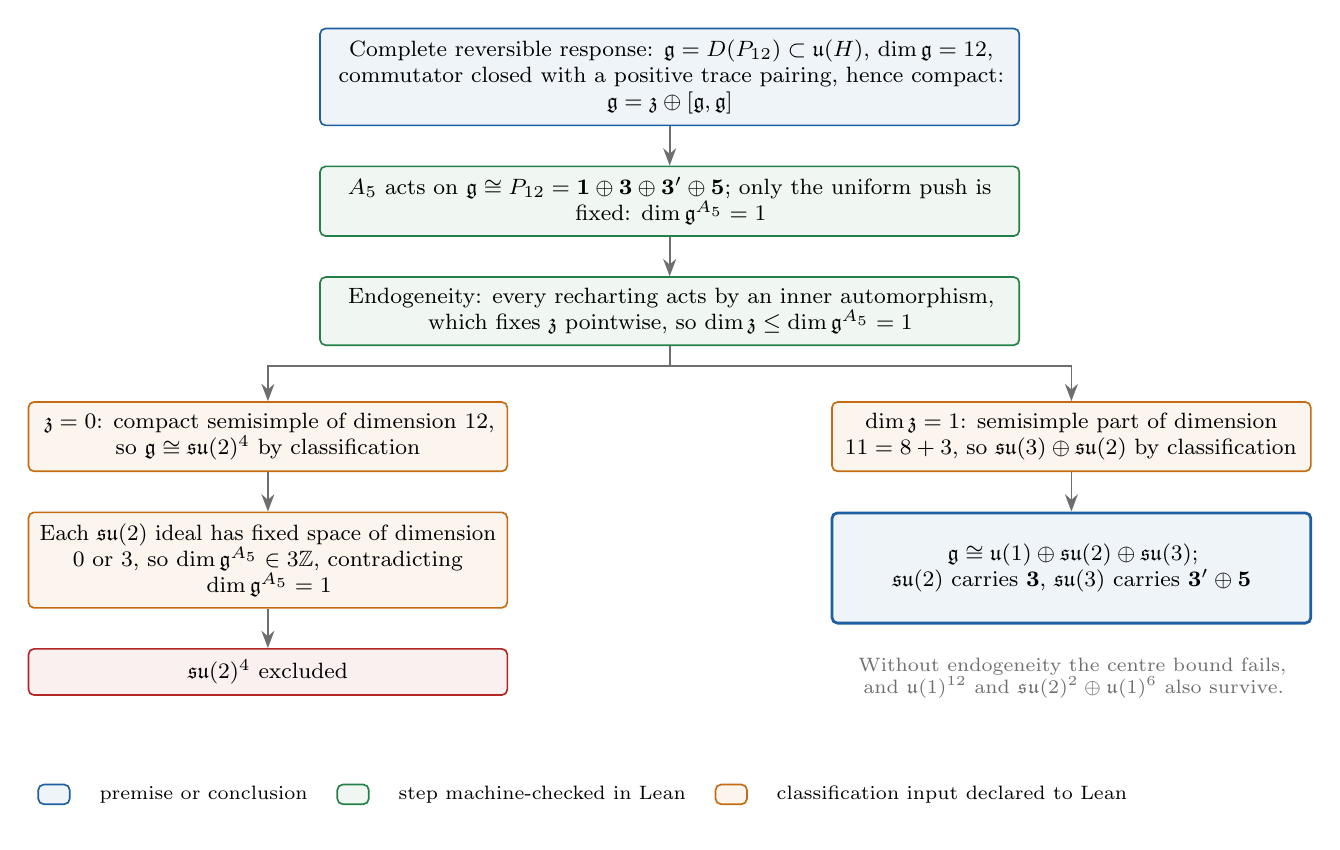
\begin{tikzpicture}[node distance=5mm and 6mm,
  step/.style={oph box=ophnative, text width=#1},
  step/.default=5.8cm,
  chk/.style={oph box=ophchecked, text width=#1},
  chk/.default=5.8cm,
  dec/.style={oph box=ophdeclared, text width=#1},
  dec/.default=5.8cm]
\node[step=8.6cm] (resp) {Complete reversible response: $\mathfrak g=D(P_{12})\subset\mathfrak u(H)$,
  $\dim\mathfrak g=12$, commutator closed with a positive trace pairing, hence compact:
  $\mathfrak g=\mathfrak z\oplus[\mathfrak g,\mathfrak g]$};
\node[chk=8.6cm, below=of resp] (fix) {$A_5$ acts on $\mathfrak g\cong P_{12}=\mathbf1\oplus\mathbf3\oplus\mathbf3'\oplus\mathbf5$;
  only the uniform push is fixed: $\dim\mathfrak g^{A_5}=1$};
\node[chk=8.6cm, below=of fix] (centre) {Endogeneity: every recharting acts by an inner automorphism, which fixes
  $\mathfrak z$ pointwise, so $\dim\mathfrak z\le\dim\mathfrak g^{A_5}=1$};
\node[dec, below left=7mm and -24mm of centre] (z0) {$\mathfrak z=0$: compact semisimple of dimension $12$,
  so $\mathfrak g\cong\mathfrak{su}(2)^4$ by classification};
\node[dec, below right=7mm and -24mm of centre] (z1) {$\dim\mathfrak z=1$: semisimple part of dimension
  $11=8+3$, so $\mathfrak{su}(3)\oplus\mathfrak{su}(2)$ by classification};
\node[dec, below=of z0] (excl) {Each $\mathfrak{su}(2)$ ideal has fixed space of dimension $0$ or $3$,
  so $\dim\mathfrak g^{A_5}\in3\mathbb Z$, contradicting $\dim\mathfrak g^{A_5}=1$};
\node[oph box=ophfail, text width=5.8cm, below=of excl] (no) {$\mathfrak{su}(2)^4$ excluded};
\node[oph box=ophnative, text width=5.8cm, below=of z1, minimum height=14mm, line width=1pt] (yes) {$\mathfrak g\cong\mathfrak u(1)\oplus\mathfrak{su}(2)\oplus\mathfrak{su}(3)$;\\
  $\mathfrak{su}(2)$ carries $\mathbf3$, $\mathfrak{su}(3)$ carries $\mathbf3'\oplus\mathbf5$};
\draw[oph arrow] (resp)--(fix);
\draw[oph arrow] (fix)--(centre);
\draw[oph arrow] (centre.south) -- ++(0,-2.5mm) -| (z0.north);
\draw[oph arrow] (centre.south) -- ++(0,-2.5mm) -| (z1.north);
\draw[oph arrow] (z0)--(excl);
\draw[oph arrow] (excl)--(no);
\draw[oph arrow] (z1)--(yes);
\node[oph label, align=flush center, text width=5.8cm, below=3mm of yes] (side) {Without endogeneity the centre bound fails, and $\mathfrak u(1)^{12}$ and $\mathfrak{su}(2)^2\oplus\mathfrak u(1)^6$ also survive.};
\matrix[below=9mm of no.south west, anchor=north west, column sep=2.5mm, row sep=1mm, nodes={font=\scriptsize, anchor=west}] (leg) {
  \node[oph box=ophnative, minimum width=4mm, minimum height=2.5mm, inner sep=0pt] {}; & \node{premise or conclusion}; &
  \node[oph box=ophchecked, minimum width=4mm, minimum height=2.5mm, inner sep=0pt] {}; & \node{step machine-checked in Lean}; &
  \node[oph box=ophdeclared, minimum width=4mm, minimum height=2.5mm, inner sep=0pt] {}; & \node{classification input declared to Lean}; \\
};
\end{tikzpicture}

\caption{Steps of the gauge Lie-type theorem. Green steps are machine-checked in the Lean library; orange steps use the classification of compact simple Lie algebras and the fixed-space argument against $\mathfrak{su}(2)^4$, which enter Lean as declared hypotheses. The port count fixes the dimension twelve by declaration; the content of the theorem is the exclusion of $\mathfrak{su}(2)^4$ and a one-dimensional centre.}
\label{fig:gauge-lie-type}
\end{figure}

The finite argument constructs its compact current inside the premise A1 unitary
response space; an ambient continuous gauge group is absent from its premises.
Write \(\mathfrak g=D(\mathbb R^{12})\subset\mathfrak u(H)\). Faithfulness gives
\(\dim\mathfrak g=12\), and commutator closure makes \(\mathfrak g\) compact
reductive. The transitive action of the alternating group on five letters,
\(A_5\), gives \(\dim\mathfrak g^{A_5}=1\). Premise A2 implements that action
internally on the same response, so it fixes the centre pointwise and
\(\dim Z(\mathfrak g)\leq1\). A centreless compact algebra of dimension twelve
would be \(\mathfrak{su}(2)^4\). Its factorwise inner \(A_5\) action has fixed
dimension zero or three on each factor and cannot have a one-dimensional fixed
space. The centre therefore has dimension one, while the semisimple part has
dimension eleven. Compact-simple classification gives the unique split
\(11=3+8\), which proves
\[
\mathfrak g\cong
\mathfrak u(1)\oplus\mathfrak{su}(2)\oplus\mathfrak{su}(3).
\]
The carrier identity \(10J=A^3-4A^2-5A+10I\) and target-blind readback derive
\(R=-J\). They do not construct the current derivative. The Lie-type theorem
uses the complete-response clauses of A1 and the endogenous-transport clauses
of A2. The port count fixes the dimension twelve by declaration. Both clauses
are hypotheses of this classification. The registered single-recurrence
interface does not produce them; its response is the commutative algebra
below. The protected native-object response considered separately below
uses a different, explicitly declared coherent-control interface. The content of
the theorem is the exclusion of \(\mathfrak{su}(2)^4\) and a one-dimensional
centre. A descent repair law enters only when a branch asks for settled public
records. It is not an undeclared premise of the Lie-type theorem. The
dimension arithmetic, the centre bound and the dimension-six exclusion used by
the Lie-type classification are machine checked in the accompanying Lean
development~\cite{ophrepo}; the \(\mathfrak{su}(2)^{4}\) fixed-space step and
the compact-Lie classification enter Lean as declared hypotheses, and no source
current or full Lie-algebra isomorphism is constructed there. The registered
formal interface keeps these inputs separate: an injective port-response map
supplies dimension twelve; an inner carrier action fixes the centre, placing
it inside the one-dimensional fixed space; the fixed-space exclusion supplies
nonzero centre; and compact-simple classification supplies the allowed simple
dimensions \(3,8,10\). The final Lean selection theorem takes the last three
dimension constraints as hypotheses and proves the split. An observable
relative phase alone establishes neither centrality nor trivial carrier
action on the entire centre, and cannot replace those hypotheses. The
formal source records that centre-triviality was found by working backwards
from the desired Lie type; the proof establishes sufficiency, not an
independent physical origin for that condition.
The registered recurrence generates the exact commutative
algebra \(\operatorname{span}\{I,A,A^2,A^3\}\). It contains neither twelve
independent current generators nor a nonzero bracket, and its only proper
recharting is the identity. This result is bounded to the registered
single-recurrence packet. The declared matrix current is an exact conditional
witness. The target-free diagonal phase lift has twelve independent first
derivatives and an abelian bracket. Adding the registered connected adjacency
tangent generates \(\mathfrak u(12)\), with derived rank \(143\). This exact
control rejects that direct lift and leaves non-diagonal source responses in
play. The canonical scalar seam equalizers do not fill that gap. On the
eleven-dimensional zero-sum port space, exact closure gives
\[
 \operatorname{rank}\langle [G_e,G_f]\rangle=49,
 \qquad
 \operatorname{Lie}\langle [G_e,G_f]\rangle=\mathfrak{so}(11),
 \qquad
 \operatorname{Alg}\langle G_e\rangle=\operatorname{End}(\mathbb R^{11}),
\]
of dimensions (49), (55), and (121), respectively. Thus the scalar
strict-descent repair maps cannot be relabelled as the desired
twelve-dimensional compact reversible current. This exact negative control
leaves a separately derived reversible response in play and prevents the
repair law from acquiring gauge content by definition.

The native binary load-two carrier supplies a more direct persistent-object
bridge. Its thirty-six nonedge pairs admit two source-derived equivariant
perfect-matching colorings by the six antipodal axes. Each normalized matching
code has dimension six, carries the actual port-permutation representation
\(1\oplus5\), and corrects every complete recorded C/E branch on all thirty
native seams with the declared coherent encoder and record-dependent recovery.
Its sum-zero quintet is protected. Two such corrected objects contain a unique
geometric \(3\oplus3'\) sector under simultaneous actual port rotations, with
an exact intertwiner inside the full thirty-six-dimensional product code.
This identifies a persistent geometric carrier; it does not supply a
spin-half lift, an exterior matter module, or autonomous selection of that
sector.

On opposite coloring choices, the twelve corresponding-port exchanges on
all \(10626\) native load-four configurations yield six independent Hermitian
mixed responses that preserve this geometric sector. They are derived using
the declared joint-code phase control; they are not copied from the
conditional gauge-current matrices. Their exact real Lie closure is
\[
 \mathfrak g_{\mathrm{native}}
 =\mathfrak{su}(3)\oplus\mathfrak{su}(3)
   \oplus\mathbb R\,iI_6,
 \qquad \dim\mathfrak g_{\mathrm{native}}=17.
\]
The actual proper port rotations belong to this connected response group at
the effective-algebra level. Finite native response words, their errors and
current readout remain separate operational obligations. This establishes a
same-object endogeneity bridge, while leaving A1's complete faithful
twelve-port response uninstantiated. In particular, conjugation on
\(\operatorname{End}(\mathbb C^6)\) sees sixteen directions: its common
scalar phase is silent on that algebra. Coherence with the retained product
complement can expose a relative phase on a larger accessible algebra.
The same preserving response menu has nine independent Hermitian operators
on the full product code, with a three-dimensional restriction kernel;
its full Lie closure therefore has dimension at least twenty and its
conjugation-visible response on \(\operatorname{End}(\mathbb C^{36})\)
has dimension at least nineteen. This enlarged interface also fails the
complete twelve-direction requirement. The present current lacks the
conditional fixture's relative phase between \(3\) and \(3'\), and it allows
five traceless phase directions on each triplet. Restricting one triplet's
phase directions does not by itself supply that missing relative current.
The native-object and response producers retain these distinctions rather
than identifying the seventeen-dimensional response as the Standard Model
gauge law.\footnote{\raggedright Exact constructions and retained checks:
\texttt{model/common\_source/native\_gauge\_object.py} and
\texttt{model/common\_source/native\_persistent\_response.py}.}

A distinct specified coherent law realizes the conditional current interface
on this same protected object without changing its ports or C/E instruments.
For the actual native port vectors \(v_p\), Galois conjugation \(\sigma\), and
cross-product matrix \(\widehat v\), choose
\[
 D_p=\operatorname{diag}\left(
 \widehat{v_p/2}+iQ_p,\widehat{\sigma(v_p)/2}\right),
 \qquad Q_p=\tfrac12v_pv_p^T-\tfrac16\lVert v_p\rVert^2I_3+
 \tfrac1{12}I_3.
\]
The native near-fivefold class sum distinguishes the two triplets before
the complex-versus-real control choice is applied. Exact checks give rank
twelve, all sixty-six bracket closures and all seven hundred twenty port
covariance identities. Proper carrier rotations belong to the same connected
current group. The sum of the currents is
\(\operatorname{diag}(iI_3,0)\), whose relative phase is observable by
cross-triplet readout. The resulting law has algebra
\(\mathfrak u(3)\oplus\mathfrak{so}(3)\). Source words execute its primitive
currents, and selected currents are composed with the geometric preparation,
native repair, record-assisted recovery and pointer outputs.
This construction changes the coherent law; it does not truncate the
seventeen-current exchange closure. Completeness is over the specified
current-control menu. The universal compiler and detector services remain
declared apparatus, and excluding their operations from that menu does not
establish their physical inaccessibility, full physical A1 closure or gauge
redundancy. Its weak double cover and exterior matter sector are separate
chosen attachments.\footnote{\raggedright
\texttt{model/common\_source/native\_sm\_current.py} and
\texttt{model/common\_source/native\_matter\_attachment.py}.}

\paragraph{Carrier rechartings and physical rotations.}
The port action above is a finite carrier symmetry. Its inclusion in the
current group is established for the stated interface; its identification
with spatial rotations of a recovered interacting field is not. The local
rank-three Gram band and the refining global low band are distinct: the
former has a fixed nonzero carrier energy, whereas the latter concentrates
on cell averages. Equivalent \(A_5\) triplets can also occur on different
tensor factors. In particular, the specified family-feedback construction
uses a gauge-trivial ancillary triplet rather than the coloured current
triplet. Representation equivalence alone therefore proves neither an
identification nor independence of physical colour, family and spatial
actions.

The conditional Spin--matter join constructs commuting actions on
\(\mathbb C^2\otimes\mathbb C^{15}\), with physical-spin central element
\(-I\) on all thirty states. The diagonal locked action instead has fourteen
minus and sixteen plus central eigenvalues and fails that fermionic test.
An explicitly chosen compensating internal transport realizes the independent
Spin action. These are finite existence and obstruction results under a
chosen tensor attachment, not a source-selected spacetime connection or a
joint charged propagator.\footnote{Public implementations:
\path{model/common_source/slow_geometry.py},
\path{model/common_source/native_repair_mass.py},
\path{model/physical_space_time/OCCUPATION_FIELD.md}, and
\path{model/observer_particles/spin_matter_join.py}.}
The remaining test must identify rotations operationally on the same
clocked field response, establish their independence from internal currents
up to the declared gauge equivalence, and check that the dynamics preserves
that identification. Coleman--Mandula separation is a constraint on a
physical scattering theory under its Poincar\'e, spectrum, analyticity and
nontrivial-scattering hypotheses; those hypotheses have not been established
for this finite interface, so no violation of that theorem follows here.\footnote{
S.~Coleman and J.~Mandula, ``All Possible Symmetries of the \(S\) Matrix,''
\emph{Physical Review} \textbf{159}, 1251--1256 (1967),
\url{https://doi.org/10.1103/PhysRev.159.1251}.}

As a counterfactual, identify the twelve ports in antipodal pairs. The
inherited quotient triangulates the real projective plane, with six
vertices, fifteen edges and ten triangular surface faces; its edge graph \(K_6\) has twenty
3-cycles. Its transitive \(A_5\) action retains one fixed line. If a
six-dimensional compact current is required to carry that action internally,
a one-dimensional centre leaves the impossible semisimple dimension five,
whereas a zero-dimensional centre gives \(\mathfrak{su}(2)^2\) and fixed
dimension zero, three or six. Thus no current satisfies all those premises.
The adjacency spectrum \(5,-1\), with multiplicities one and five, is
exactly the antipode-even part of the icosahedral spectrum; the two
\(\pm\sqrt5\) triplets are antipode-odd. The executable named-menu table
at \path{code/discriminator_strata/carrier_specificity.py} checks these
finite facts. Antipodal identification changes topology and port count;
forgetting a chosen orientation alone leaves the twelve-port sphere.
This comparison supplies neither a calibrated specificity score nor a
physical current attachment.


Conditional on the canonical oriented carrier, the complete target-free
space \(\operatorname{Hom}_{A_5}(\Lambda^2\mathbb Q^{12},\mathbb Q^{12})\)
has dimension fourteen and an exact rational Reynolds basis. It is a search
space only; no bracket is selected. Substitution of the general bracket into
Jacobi gives 2,640 coordinate equations in 44 target orbits and an exact
coefficient-row rank of 38. A channel change over \(\mathbb Q(\sqrt5)\)
splits that rowspace into eleven fixed-line derivation-weight products and a
rank-27 residual system. The residual equations apply on every weight flat.
A three-parameter derivation-only Jacobi family is exact and supplies no
compactness or source selection. The compact real locus of that
fourteen-parameter equivariant variety is classified, conditional on
three named textbook lemmas and exactly over \(\mathbb Q(\sqrt5)\), into
three certified bracket families, and for each family the coroot lattices,
integral carrier weights, and carrier-admitted mathematical global form are computed
exactly; the selected forms are adjoint with zero abelian charge lattice, so
the abelian sector is undetermined at carrier level and stands exposed
rather than repaired.

The source incidence admits a particularly sharp finite discriminator.
Applying the declared equal-weight cyclic rule to its twenty oriented faces
gives
\[
 B_{\rm face}=60R_{13}.
\]
This bracket is \(A_5\)-equivariant but fails Jacobi in exactly \(240\) of
the \(2640\) independent coordinates, split \(120\) at \(+1\) and \(120\)
at \(-1\). Under the explicitly added Euclidean metric on upper-triangular
structure constants, orthogonal projection onto the complete compact locus
has the unique nearest family \(G\):
\[
 d_G^2=\frac{615-123\sqrt5}{22},\qquad
 d_F^2=\frac{615+123\sqrt5}{22},\qquad d_P^2=45 .
\]
Both \(F/G\) projections lie in their certified open compact strata. The
same conclusion is exact for two endpoint edit norms on the identical
792-coordinate convention. Exact primal--dual certificates give
\[
\begin{aligned}
 d_1(G)&=30(\sqrt5-1)
   < \inf d_1(F)=d_1(P)=60,\\
 d_\infty(G)&=\frac{5-\sqrt5}{10}
   <d_\infty(F)=\frac{\sqrt5}{5}
   <d_\infty(P)=\frac12.
\end{aligned}
\]
The \(G\) optimizers lie in its open compact stratum. The displayed
\(\ell_1\) value for \(F\) is an infimum, not an attained minimum: the zero
point minimizes the ambient linear family and compact \(F\) points approach
it under scaling. The exact Python replay proves the 792-coordinate
primal--dual optimization; the Lean theorem checks the serialized radical
values and their strict order. Thus the family verdict is robust across
total, quadratic, and worst-coordinate edit scores, but only on the
classified compact locus and only after the coordinate norm is supplied.
The equal-weight rule and the coordinate norms are declared inputs rather than
consequences of A1--A3, so the verdict is a conditional discriminator
obtained without reference to the measured value.

The quadratic verdict is additionally metric-robust over the complete
invariant class. The carrier splits multiplicity-free as \(1+3+3'+5\), and
the commutant of the port action is exactly four-dimensional, spanned by the
four symmetric spectral projectors; hence every invariant carrier inner
product is a positive sector-scale metric
\(\alpha P_1+\beta P_3+\gamma P_{3'}+\delta P_5\), and every induced
Hilbert--Schmidt metric on structure constants is diagonal across the
fourteen equivariant channels. The squared distances from \(B_{\rm face}\)
to the classified compact families are the exact closed forms
\[
\begin{aligned}
 d_P^2&=\frac{15-3\sqrt5}{\beta}+\frac{15+3\sqrt5}{\gamma}
   +\frac{15-3\sqrt5}{2}\,\frac{\beta}{\delta^2}
   +\frac{15+3\sqrt5}{2}\,\frac{\gamma}{\delta^2},\\
 d_F^2&=\frac{15+3\sqrt5}{2}\,\frac{\gamma}{\delta^2}
   +\frac{15+3\sqrt5}{\gamma}+\frac{60+12\sqrt5}{11\beta},\qquad
 d_G^2=\frac{15-3\sqrt5}{2}\,\frac{\beta}{\delta^2}
   +\frac{15-3\sqrt5}{\beta}+\frac{60-12\sqrt5}{11\gamma},
\end{aligned}
\]
with \(\alpha\) absent. Both gaps \(d_P^2-d_G^2\) and \(d_P^2-d_F^2\)
are coefficient-positive Laurent polynomials, so \(P\) is strictly
excluded for every invariant carrier metric. At \(\gamma=\beta\) the gap
is \(d_F^2-d_G^2=3\sqrt5\,\beta/\delta^2+(90\sqrt5/11)/\beta>0\), so
every sector-balanced metric selects \(G\); and for every metric with
\(\beta/\delta\in[1/50,6]\) the family \(G\) stays uniquely nearest for
all \(\gamma\) and \(\delta\). The mirror family \(F\) genuinely takes
over on the \(d_F^2<d_G^2\) side of the exact three-scale tie surface, with witness
\((\beta,\gamma,\delta)=(8,1,1)\). Conjugating \(\sqrt5\) and swapping
\(\beta\leftrightarrow\gamma\) maps \(d_G\) to \(d_F\) exactly: the
\(F/G\) asymmetry is the Galois image of the sector swap. Reversing every face
orientation negates \(B_{\rm face}\) but leaves these distances unchanged,
because the compared compact families are centrally symmetric; orientation
therefore does not select the branch. A channel-diagonal invariant metric on the bracket space that is not
carrier-induced reverses the balanced-point selection, so the
carrier-induced restriction is load-bearing. The exact replay derives the
closed forms from the pinned tensors and replays six sample metrics through
raw normal equations; the Lean companion proves the exclusion, balanced,
box, and witness statements as quantified real theorems over the closed
forms. The nearest-point law and the carrier-induced class are declared
discriminator choices. The committed dual-measure layer adds a
measure-conditional point: on the pinned incidence table, equal normalized
face weights and the declared barycentric one-third share give port-dual
weight exactly \(1/12\) at every port, and under the declared diagonal
measure-to-metric rule that uniform measure induces the scalar carrier
inner product at the balanced cone point \((1/12,1/12,1/12,1/12)\), where
\(G\) is uniquely nearest with \(d_G^2=(3690-738\sqrt5)/11\),
\(d_F^2=(3690+738\sqrt5)/11\), and \(d_P^2=540\), twelve times the
reference distances by the exact scaling identity
\(c\,d^2(c,c,c)=d^2(1,1,1)\). The weighting rules and the measure-to-metric
identification are declared, so this upgrades the metric-conditional
selection to a measure-conditional selection whose measure is pinned by a
committed theorem; it is not source selection of the bracket or a physical
gauge structure. One composed machine-checked surface
(\texttt{Lean/Screen/SMStructureAdequacySurface.lean}) bundles the
declared weighting, metric, classification-input, and exterior-selection
premises and re-exports the premise-implied Lie type, the balanced-point selection,
the one-generation exterior selection with anomaly cancellation, and the
conditional global-form menu as one package, with the same-source
loop-to-kernel identity named as the leading undischarged clause of the
physical quotient. A companion composition
(\texttt{Lean/Screen/SMStructureComposition.lean}) closes the
side-by-side gap in that package: one theorem on the one premise bundle
proves that the premise-implied type admits a unique type-matched nearest family
at the bundle's balanced point and that the fifteen-state count, the
anomaly forms, and the \(\mathbb Z_6\) stabilizer are carried by the
bundled selection mask itself. Its capstone is a coarse two-mask statement:
among the three classified family labels and the declared \(2^{10}\)
exterior table, the admissible pairs are the \(G\) label with either of two
conjugate masks. Conjugation is proved on the masks only. This does not count
points in the continuous \(G\)-bracket family and does not classify complete
physical Standard Model structures.

The descent bookkeeping itself is exact. On the finite weight lattice of
hypercharge, triality, and duality labels in the \(q=6Y\) normalization, a
label is fixed by every element of the diagonal \(\mathbb Z_6\) kernel
exactly when \(2t+3d+q\equiv 0 \pmod 6\); the kernel acts on any label by
multiples of this center character. Every row of the matter table satisfies
the congruence, including both carrier blocks and the scalar, a fractionally
charged singlet is blocked by the generator, and exactly one sixth of the
thirty-six lattice labels descend, with every character value carried by
exactly six labels. The machine-checked receipt composes onto the selected
matter mask: every selected component descends through the full kernel
(\texttt{Lean/Screen/GlobalFormCharacterDescent.lean}). This is the
character-lattice half of the global-form question only. The complete
character category, the instanton normalization, the laboratory flux
attachment, and the selection of one physical quotient among the four
admissible ones are additional assumptions, and no physical global form is
derived from the congruence.

A three-family
bundle types the band-selection rules of the family row as antecedent
fields whose triplication arithmetic threads the same selection mask,
the chirality row carries one threaded grading-plus-obstruction
theorem, and a kernel-checked dictionary identifies the dimension-six
baryon census table with the selected generation column by column.
The construction supplies no physical-family or Spin/chirality attachment
and no source action.

For the actual four-entry band table, faithfulness excludes the
dimension-one trivial band; the remaining dimensions are \(3,3,5\).
Removing the stated window while retaining that table and faithfulness
therefore changes no admissible candidate. The conditional physical window
does not itself explain triplication. The load-bearing identification is
that the family object is a single complete faithful adjacency band, compared
by the declared cost rule and realized in the proposed matter response.

Generation names require no extra universally conserved generation charge.
Within a sector whose physical charges and statistics are established,
ordering nondegenerate masses is a naming convention. A physical comparison
must additionally retain the eigenvectors, residues and charged-current
matrix of the same response, with common permutations and phase conventions.
The mismatch of the two left quark diagonalizers determines CKM mixing;
requiring a generation label conserved by every charged weak transition
would exclude that mixing.\footnote{A.~Ceccucci, Z.~Ligeti and Y.~Sakai,
``CKM Quark-Mixing Matrix,'' in the Particle Data Group review (2024),
Section 12.1,
\url{https://pdg.lbl.gov/2024/reviews/rpp2024-rev-ckm-matrix.pdf}.}
A decoder returning declared charge labels is consequently an intermediate
representation check, not a derivation of the particle content of arbitrary
ordered spectral gaps.

Over the supplied certified brackets, ad-invariance fixes the kinetic shape
block-diagonally with exactly zero cross terms. On carrier-projector forms the
restriction is stronger and exact: families \(F\) and \(G\) reduce the
three-dimensional carrier-invariant space to two dimensions,
\[
 F:\ w_{3+}=\sqrt5\,w_5,\qquad
 G:\ w_{3-}=\sqrt5\,w_5,
\]
with \(w_{3-}\) free for \(F\) and \(w_{3+}\) free for \(G\); family \(P\) is the exact
two-to-two control. Requiring one form to be invariant for both \(F\) and
\(G\) leaves the ray
\((w_{3+},w_{3-},w_5)=t(\sqrt5,\sqrt5,1)\), but simultaneous mirror
invariance is an extra premise, not source selection. The stored
minus-one-quarter Killing matrices are exact representatives, not selected
couplings. The two-factor history theorem constructs a Gibbs kernel from
\(a q_1+b q_2\), proves exact normalizer and kernel factorization, and recovers
the additive factor action. If both costs vary, equality of two constructed
kernels identifies \(\lambda a\) and \(\lambda b\); with nonzero multipliers
only common scaling survives, so \(a/b\) is not multiplier gauge. Exact
instances cover both \(P\) factors on \(3^6\) steps and the full
color-bearing \(F\) family on \(3^{11}\) steps. These are symbolic finite
theorems, not large enumerations. They neither identify an independent source
kernel nor select \(a\), \(b\), or their ratio.
No theorem supplies an enumeration of noncompact components, a source
repair/selection law, action selection, same-current holonomy, relative factor
coefficients, or coupling scales \cite{ophfpe,ophrepo}.
Generation, scalar, global-form, and extra-sector statements carry their own
premises.

\subsection*{An assembled structural action}

The three committed sector functionals sum as one real function of one field
tuple on one typed premise bundle
(\texttt{Lean/Screen/AssembledActionComposition.lean}). The bundle extends
the electroweak-breaking premise data by two declared positive gauge weight
parameters in the committed two-parameter \(G\)-invariant normal form, and
the assembled action is the explicit sum of a gauge kinetic term (one
declared magnitude per invariant carrier sector, squared against its weight
under a declared diagonal pairing on the committed weight space), the
committed quartic potential \(\lambda(|h|^2-v^2)^2\), the committed gauge
mass form at the chosen minimum, and the realified committed Yukawa line
with coefficient \(y\). Three exact restriction theorems recover each
committed sector functional on its field slice over the common base tuple.
The assembled gauge coefficients satisfy the committed \(G\) ad-invariance
constraint row and collapse to the committed one-ray mirror form under the
extra declared \(F\) row. The whole sum is exactly invariant under the
global abelian phase action at unit scalars with product one, in particular
at the committed integer charge balance of the bundled selection mask, with
the scalar slot at plus or minus the committed scalar row charge. The
imaginary part of the committed complex Yukawa line is recovered as an
assembled evaluation, the base tuple evaluates to zero, and the bundle is
inhabited with every declared parameter equal to one. This is a finite
structural action on the committed coarse grammar: every coefficient is a
declared bundle parameter, the covariant kinetic content enters only through
the committed constant-direction coefficient at the minimum, and the
construction supplies no source-produced spacetime action, measured
coefficients, three-physical-family attachment, global-form selection,
physical-chirality attachment, or Spin attachment.

\subsection*{The gauge sector at the committed invariant-form level}

The gauge kinetic sector of the assembled action extends from the declared
diagonal pairing to the committed invariant-form level
(\texttt{Lean/Screen/GaugeSectorBracketCompletion.lean}). The typed
gauge-field slot carries one real coordinate vector per weighted invariant
carrier sector of the committed multiplicity-free split \(3^+ + 3^- + 5\),
and the kinetic functional is the committed weight vector against the
sector coordinate squared norms. The declared diagonal pairing is exactly
the axis restriction of this functional under the committed basis, the
functional factors exactly through the committed pairing at the sector
magnitudes, and agreement on the axis slice pins the weights, so the
assembled action embeds exactly in the completed one and the completed
action factors exactly through it. The invariance is carried at the exact
infinitesimal grade: every sector-internal skew-adjoint generator leaves
every weight vector invariant, the committed \(G\) and \(F\) ad-invariance
constraint rows are the infinitesimal-invariance rows of two exhibited
cross-sector generators at declared coefficient ratio \((1, -\sqrt{5})\),
and simultaneous invariance under both leaves exactly the committed
one-ray mirror family. The restriction, abelian-invariance,
committed-charge, and base receipts persist, the parameter census is
unchanged at exactly the two declared normal-form parameters, one
exhibited off-axis carrier point evaluates outside the axis slice, and the
control weight vector \((1,1,1)\) breaks the invariance at an exhibited
carrier pair with exact value \(1 - \sqrt{5}\). No gauge group action on
the carrier is committed or claimed; the generator ratio realizes the
committed constraint rows, its derivation from the pinned bracket tensors
is certificate content, and no source-produced spacetime action is supplied.

\subsection*{A fermion sector on the assembled action}

The assembled action carries one typed fermion sector as a fourth summand,
with the committed sum unchanged
(\texttt{Lean/Screen/FermionSectorAssembly.lean}). The fermion carrier is
one complex amplitude per row of the committed ten-component table, and the
bilinear row-pair form \(\overline{\psi_i}\,\psi_j\) transforms under the
abelian phase action through the committed integer charge column
\(q = 6Y\). On the rows of the bundled selection mask the form is invariant
at every unit phase exactly when the committed row charges balance, and the
committed charge column separates those rows, so the invariant pairs are
exactly the diagonal ones: the charge column forces the kinetic-shaped
pairing to be diagonal. The extended action is the committed assembled sum
plus the masked diagonal fermion sector with one declared coefficient per
row. It restricts exactly to the committed assembled action on the zero
fermion slot and at zero fermion coefficients, exactly to the fermion
sector on the fermion slice, and the three committed sector restrictions
persist. A typed embedding of the fermion amplitudes at the shared doublet
and singlet rows into the committed matter slots evaluates the extended
action to the committed mass bilinear with coefficient \(y\,v\), and the
embedding intertwines the fermion phase action with the committed
matter-slot phase action at the committed row charges. The extended sum is
exactly invariant under the committed-charge abelian action extended by the
fermion charge phase, the parameter census is the committed list plus the
fermion coefficients, the bundle is inhabited over the committed
inhabitant, and an exhibited charge-imbalanced pair of mask rows breaks the
invariance receipt at an exhibited unit phase. The fermion coefficients are
declared stand-in weights: the covariant kinetic term, the source-produced
spacetime action, and the Spin and physical-chirality attachments are not
supplied, and no measured coupling, three-family structure, or Yukawa
matrix appears.

\tableofcontents
\clearpage

\def\OPHSkipEinsteinChain{1}
\def\OPHStandardModelDerivationPaper{1}
\def\OPHSkipEmbeddedReferences{1}
\section{Matter and interaction readout from the finite response}
\label{sec:repair-matter-readout}

The finite response determines more than the abstract gauge Lie type. Its
matrix generators support an exact, conditional matter decoder and local
interaction tensors. A representation is distinct from a physical particle:
a particle identification also consumes its spin, statistics, propagator,
interaction and observer-clock interpretation.

\subsection{From response operators to a fifteen-state matter module}

Let a response generator on the six-dimensional carrier have blocks
\(D=\operatorname{diag}(A,B)\), with \(A\in\mathfrak u(3)\) and
\(B\in\mathfrak{so}(3)\). Write \(B=\widehat w\). The declared spin lift and
central trace redistribution give
\[
 L(D)=\operatorname{diag}\left(
 A,-\frac{i}{2}w\cdot\sigma-\frac{\operatorname{tr}A}{2}I_2\right).
\]
This is a Lie-algebra homomorphism. The complete twelve-direction response
and all sixty-six bracket pairs are checked exactly. The central direction,
after clearing denominators and choosing the weak-positive orientation, has
primitive integer character
\[
 q=\operatorname{diag}(-2,-2,-2,3,3).
\]
The lift and trace redistribution are hypotheses. A native weak rotation
through \(2\pi\) is the identity on its vector carrier and acts as minus the
identity on the lifted doublet. Thus the lifted module is not a
subrepresentation of the original six-dimensional response. Global descent
and a physical current interpretation require the corresponding additional
identifications.

\begin{proposition}[Conditional matter decoder]
For the lifted five-dimensional one-body action, the representation
\[
 M=\Lambda^2\mathbb C^5\oplus\Lambda^4\mathbb C^5
\]
has dimension fifteen. Its charge and quadratic Casimir operators identify
the following irreducible components without a field-name input table.
\end{proposition}

\begin{center}
\begin{tabular}{ccccc}
\toprule
Component & Color & Weak dimension & \(Y=q/6\) & Dimension\\
\midrule
\(Q\) & \(3\) & \(2\) & \(1/6\) & \(6\)\\
\(u^c\) & \(\overline3\) & \(1\) & \(-2/3\) & \(3\)\\
\(d^c\) & \(\overline3\) & \(1\) & \(1/3\) & \(3\)\\
\(L\) & \(1\) & \(2\) & \(-1/2\) & \(2\)\\
\(e^c\) & \(1\) & \(1\) & \(1\) & \(1\)\\
\bottomrule
\end{tabular}
\end{center}

\begin{proof}
Split \(\mathbb C^5=V_c\oplus V_w\), of dimensions three and two and
charges \(-2\) and \(3\). Then
\[
\Lambda^2(V_c\oplus V_w)=\Lambda^2V_c\oplus(V_c\otimes V_w)
 \oplus\Lambda^2V_w,
\]
with integer charges \(-4,1,6\). The degree-four summands are
\(\Lambda^3V_c\otimes V_w\) and
\(\Lambda^2V_c\otimes\Lambda^2V_w\), of charges \(-3,2\).
Color and weak Casimirs separate the representations, and Cartan weights
distinguish the conjugate color character. Exact projectors give the same
answer after a rational change of basis mixing unlike charge sectors.
\end{proof}

The auxiliary exterior construction has two additional invariant lines, the
vacuum and top exterior degree. Removing them is part of the declared
fifteen-state module. Charge traces alone do not remove neutral invariant
states. Its even auxiliary parity also does not establish physical fermion
statistics. Physical two-component Weyl fields require an independent CAR
algebra and spin interpretation. The anomaly-free charge table and common
central kernel are conditional representation results; they do not identify
laboratory species or select a generation count.

\subsection{One Higgs doublet and the exact interaction tensors}

For two same-chirality physical Weyl fields, the antisymmetric spinor
contraction makes the internal coefficient symmetric. The Lorentz-scalar
internal pair space is consequently \(\operatorname{Sym}^2M\), of dimension
120. A color-Casimir kernel and weak-Casimir projector identify one doublet
of hypercharge \(-1/2\) and two of hypercharge \(+1/2\). Their constituent
integer-charge pairs are \((-4,1)\), \((-3,6)\), and \((1,2)\).
These are interpolating channels; their existence supplies no bound-state
pole, condensate or elementary-boson commutation relation.

\begin{proposition}[Conditional one-doublet interaction]
Declare one scalar doublet \(H\) of hypercharge \(1/2\). Each of the three
channels above has a one-dimensional invariant contraction space. They give
\[
 Q u^c H,\qquad Q d^c H^*,\qquad L e^c H^*.
\]
The same scalar doublet and its conjugate occur in all three expressions.
\end{proposition}

\begin{proof}
Restrict the exact pair generators to each color-singlet doublet. The tensor
sum of that doublet generator and the generator of \(H\), or its conjugate,
has a one-dimensional common kernel. Equivalently, its coefficient matrices
\(C_\alpha\) satisfy, for each of the twelve source currents,
\[
 T^t C_\alpha+C_\alpha T+
 \sum_\beta(T_H)_{\beta\alpha}C_\beta=0.
\]
Here the conjugate action is \(-T_H^t\) in the skew-Hermitian convention.
The physical pairing kernel \(\epsilon\otimes C_\alpha\) is antisymmetric.
The identity \(S^t\epsilon S=\epsilon\) for \(S\in\mathrm{SL}(2,\mathbb C)\)
establishes its Lorentz scalar character. The executable checks the
rotation and boost generators as well as all current identities.
\end{proof}

For three declared families the coefficients are three complex
\(3\times3\) matrices, with 27 complex entries before flavor-basis
redefinitions. The pairing convention is
\[
 \mathcal L_{\rm pair}=\frac12\epsilon_{AB}
       \psi_A^tK(H)\psi_B+\mathrm{h.c.}
\]
up to an overall sign. With canonical kinetic normalization and
\(H=(0,v)\), its singular values are tree-level mass parameters;
\(v=v_{\rm SM}/\sqrt2\) in the conventional electroweak normalization.
Exact matrix-unit tests cover arbitrary complex family coefficients.
Their values, the Higgs potential and its vacuum are not selected by these
identities. The optional invariant \((LH)(LH)/\Lambda\) has six complex
symmetric family coefficients and gives \(M_\nu=\kappa v^2/\Lambda\).
It is an additional dimension-five effective interaction, with no selected
coefficient, scale or ultraviolet completion.

If both family factors are identified with the same unbroken irreducible
rank-three source representation and the Higgs is family-neutral, the exact
commutant has dimension one. In that branch each Yukawa intertwiner is
\(yI_3\), giving equal singular values. A nonscalar background can split the
band; choosing that background is an additional physical hypothesis. The
source family-band theorem therefore does not imply the observed hierarchy.

\subsection{Scope of the readout}

A declared coherent filter on the native six-dimensional response admits an
exact invertible twelve-control map into the same compact algebra; the
spin/exterior and Higgs tensor maps above apply after this change of controls.
It must not be identified with state cooling. For a rank-three projector
\(P\), the cooling channel
\(\Phi(\rho)=P\rho P+\operatorname{tr}((I-P)\rho)P/3\)
has dual \(\Phi^*(B)=PBP+\operatorname{tr}(PB)(I-P)/3\), which is not the
Hamiltonian map \(h\mapsto PhP\). Its classical recorded branches lose the
relative phase of the two triplets.

The executable calculations reconstruct the response, representation
projectors and interaction tensors from repository-local source operators,
with exact rational or algebraic identities separated from numerical
residuals. They use no measured particle masses. They supply neither a
physical chiral field net nor a source-selected Higgs vacuum, Yukawa matrix
or mass pole. A relaxation gap, finite cavity frequency or commuting
internal modular offset requires its own mass-shell identification before
it can be called a physical rest mass.


% Recovered core of the spacetime and Einstein-dynamics paper: premises,
% collar and overlap-gluing theorems, the Lorentz chain and the Einstein chain.
% The Standard Model gauge paper cites its overlap-gluing section. The file
% name is cited under this spelling by pinned manifests in code/a5_closure
% and by a frozen custody record, so it stays as it is.
\section{Recovered Core: Foundations and Structural Branches}\label{observer-patch-holography}

Observer-Patch Holography is a reconstruction program for fundamental physics. On the declared
screen-first global-support branch, physical data are charted by a horizon screen \(S^2\), and the
effective world is encoded by the mutual consistency of overlapping patch descriptions. This
support screen is distinct from a local carrier boundary and a federation overlap nerve. On the
producer branch, \(S^2\) enters only after the carrier-to-support map satisfies the spherical
incidence, mesh, cross-ratio, normalization, and refinement receipts. A finite reference
fixture without a composable seam triangle does not supply that map, since its
higher-overlap condition is vacuous. The source-derived producer supplies a
twelve-chart, thirty-seam, twenty-face incidence nerve, nonvacuous seam-triangle cocycles,
confluent phase repair, and a controlled oriented-\(S^2\) support limit on one declared tower.
Event, modular, scale, and laboratory attachments require separate premises.

This recovered-core section develops fixed-cutoff overlap repair, collar recovery, overlap
gluing and its transport obstructions, and the geometry-readout route to Lorentz frame
kinematics and conditional Einstein dynamics.

\subsection{Overview}\label{overview}

Theorem, lemma and section numbers inside this recovered core, such as
Theorem 4.2 or Section 2.3, follow the core's own internal numbering, not the
section numbering of the surrounding paper.

Overlap consistency turns local patch states into a constrained gluing problem. The
fixed-cutoff branch gives collar decompositions, edge centers and finite repair dynamics on the
declared physical quotient (Sections 2--3). Modular flow on caps supplies Lorentz-frame
kinematics and the three-dimensional observer-frame hyperboloid (Section 4). Certified
read-from provenance generates a finite informational poset and its longest
authenticated-parent-chain height; the rank-three source Gram quotient and a real axis define
the ambient \(1+3\) target carrier, and source height enters only through the temporal
coordinate of a scaled event placement. Positive null translations supply directional charges,
finite null tomography reconstructs a symmetric tensor, and fixed-cap generalized-entropy
stationarity with the stress, small-ball, coupling, vacuum and scale premises implies the
Einstein equation (Section 5). Bare finite consensus stops at quotient normal forms, and the
cap-normal \(H^3\) chart stops at observer frames; neither populates a spacetime.

The selected no-\(G\) scale certificate enters only the Newton-constant readout. The
source-causal continuum and Einstein theorems do not depend on the matter or sector-completion
branches.

\subsection{Model and Premises}\label{1-model-and-axioms}

\subsubsection{Observers and access model}\label{11-observers-and-access-model}

The support-local algebra-state-record reduct of an observer patch is
\(O_{\mathrm{red}}=(P_O, \mathcal{A}(P_O), \rho_O, R_O)\), where:

\begin{itemize}
\tightlist
\item
  \(P_O \subset S^2\) is a connected screen patch (the observer\textquotesingle s access region).
\item
  \(\mathcal{A}(P_O)\) is the von Neumann algebra associated to \(P_O\).
\item
  \(\rho_O\) is the local state, obtained by restricting the global state to \(\mathcal{A}(P_O)\).
\item
  \(R_O\) is a finite record algebra generated by stable internal record projectors within \(P_O\).
\end{itemize}

An operational observer additionally carries overlap interface algebras and restriction maps,
allowed update and repair instruments, and checkpoint data used for continuation. Observers are
internal self-reading patterns in the global state. A patch and its compatible marginal supply a
geometric or algebra-state chart. An operational observer requires the interface, record, repair,
and checkpoint conditions.

\subsubsection{Screen, patches, and algebra net}\label{12-screen-patches-and-algebra-net}

We work in a single static patch with a horizon screen \(S^2\). Each connected subregion \(P \subset S^2\) is assigned a von Neumann algebra \(\mathcal{A}(P)\). The net satisfies isotony:

\[
P \subset Q \implies \mathcal{A}(P) \subset \mathcal{A}(Q).
\]

A global state \(\omega\) is a positive linear functional on the inductive-limit algebra. Overlap consistency is imposed algebraically: for overlaps \(P_1 \cap P_2\), \(\omega\) restricted to \(\mathcal{A}(P_1 \cap P_2)\) is the same from either side.

\subsubsection{The premises A1--A3}\label{13-premises}

This paper states the premises A1--A3 of the observer-overlap foundation. The flagship synthesis~\cite{ophflagship} gives the account of the theory, and the executable observer paper~\cite{ophmodel} records which of these premises the construction supplies. Branch-local hypotheses are written at the theorem that consumes
them.

The support-visible BW scaling theorem handles the scaling step. The source-causal continuum and Einstein
theorems use the additional collar-recovery, edge-normalization, generalized-entropy,
common-domain, stress, scaling, universal-coupling, vacuum-reference, and scale-readout
interfaces stated in their own hypotheses; none of those interfaces belongs to A1--A3.

The screen premise A1 below defines the screen-first support branch. The producer branch reaches the
same premise only after its carrier-to-support receipts establish the global support screen.

% Shared panel of the theorem premises A1--A3. Included by papers that state
% the premises in full. Canonical machine source: claims/axiom_registry.yaml;
% reviewed reference: docs/AXIOM_REFERENCE.md. Do not hand-copy a competing
% formal block into a paper; include this fragment.

\paragraph{A1 (oriented observer-patch federation and spherical support).}
There exists an observer patch net on an oriented spherical screen: at every
finite resolution each local carrier has twelve primitive boundary ports
forming the vertices of an oriented triangular boundary with 30 edges and 20
faces, combinatorially the boundary of an icosahedron, and carriers join
through typed seams and coherent triple overlaps, refine to an oriented
spherical support, and expose local state, readback, records, repair moves,
and checkpoints. Their complete infinitesimal port response is represented
faithfully on a finite-dimensional unitary response space and is closed under
the commutators generated by ordered response composition. Formally, for
every regulator \(r\) in a
directed system there is a typed object
\(\mathfrak N_r=(\mathcal P_r,\mathcal A_r,\mathcal R_r,\mathcal I_r,
\mathcal U_r,\mathcal C_r,N_r,S_r,b_r)\):
a finite patch/overlap category with an isotone local algebra net and
central record algebras; a federation of finite carriers, each with twelve
primitive pairwise-orthogonal central port projections summing to one and a
boundary packet \(K=(P,E,F,o)\) with \(|P|=12\), \(|E|=30\), \(|F|=20\),
degree-five ports, five-cycle links, and coherently oriented two-face edges,
isomorphic to the icosahedral boundary complex with no preferred labels;
seam algebras with unital restrictions and coherent triple-overlap cocycles
forming the nerve \(N_r\); a finite edge-midpoint refinement support
\(S_r\) realized orientation-preservingly in \(S^2\) with mesh tending to
zero; and a source-bound degree-one bridge \(b_r:N_r\to S_r\), all commuting
with refinement. Each carrier also has
\(V_{r,i}=\mathbb R[P_{r,i}]\), a finite-dimensional complex Hilbert space
\(H_{r,i}\), and an injective real-linear map
\[
D_{r,i}:V_{r,i}\longrightarrow\mathfrak u(H_{r,i}).
\]
The image \(\mathfrak g_{r,i}=D_{r,i}(V_{r,i})\) is closed under
commutators and complete for the declared quotient-visible infinitesimal
port response. The primitive port probes span \(V_{r,i}\), no additional
public response direction is omitted, and
\(-\operatorname{Tr}(D_{r,i}(v)D_{r,i}(w))\) is positive definite. The
response construction is natural under admissible presentation equivalence
and refinement. A1 does not select a particular response table,
inverse-port law, Lie type, global group, particle interpretation, or metric
content.

\paragraph{A2 (observer agreement).}
Observers operating on the screen agree on the meaning of the data they
jointly interpret. Formally, the interpretation map
\(\mathcal J_r:\mathsf{Data}_r\to\mathsf{Meaning}_r\) from
observer-accessible data to operational meanings is natural with respect to
every visible overlap restriction, recharting, seam translation,
higher-overlap map, federation map, and refinement map: every declared
data-access diagram for accepted public data commutes after interpretation,
and \(\mathcal J_r\circ c_{s\to r}=C_{s\to r}\circ\mathcal J_s\) across
resolutions. A2 constrains accepted shared data only, and the domain
it quantifies over is supplied by the A1 interfaces rather than by A2
itself.

Accepted reversible overlap transports form a groupoid \(\mathcal O_r\).
For a complete carrier chart \(o\), its closed paths
\(\operatorname{Hol}_r(o)\) map onto the orientation-preserving incidence
automorphisms \(\operatorname{Aut}^{+}(K_{r,i})\). For every proper carrier
automorphism \(a\), A2 supplies a closed path \(\gamma_a\) and one
projective implementer
\([U_a]\in\operatorname{PU}(H_{r,i})\) satisfying
\[
\operatorname{Ad}_{[U_a]}D_{r,i}(v)=D_{r,i}(a\cdot v).
\]
Writing
\[
G_{D,r,i}^{0}
=
\left\langle
\exp(tD_{r,i}(v)):t\in\mathbb R,\ v\in V_{r,i}
\right\rangle^{0},
\]
the implementer is endogenous:
\[
[U_a]=[g_a c_a],
\qquad
g_a\in G_{D,r,i}^{0},
\quad
c_a\in C_{U(H_{r,i})}(\mathfrak g_{r,i}).
\]
Closed paths compose projectively and the construction commutes with
refinement. A unitary lift need not be unique. Scalar phases and centralizer
actions are permitted because they act trivially on the response algebra.
An independent spectator carrying a matching projective action cannot
replace the response-generated factor or contribute a public response
direction. The closed path, port action, and implementer must arise from the
same accepted source history in an executable realization.

The two response clauses support an abstract target-free compact Lie-type
theorem. They do not certify that an executable producer emitted a particular
current fixture. Such a certification must reconstruct the port generators,
commutator, and projective implementers from ordered source histories without
a named current model upstream. A2 does not imply global state
extension, repair termination, confluence, unique normal forms, record
durability, Byzantine safety, dissemination, or commutation of state
optimization with refinement; raw mismatch and repair precede acceptance.

\paragraph{A3 (conditional maximum randomness).}
Everything that observer agreement leaves unconstrained is maximally random.
Formally, at finite regulator \(r\) a state is a compatible family of local
normalized states on the accessible algebra net; \(\mathcal K_r\) is the
nonempty convex set of such families satisfying the finite observer-visible
constraints supplied by A1 and A2 through an A1-generated constraint
grammar with a factorization theorem; and, relative to an exact reference
family \(\tau_r\), an A1-generated observer cover \(\mathcal G_r\), and
strictly positive exact weights \(w_{r,P}\) constructed from quotient-visible
A1 data by a rule natural under admissible presentation equivalence, the
realized state is the
information projection. The cover restriction map is injective on
\(\mathcal K_r\); equivalently, at smooth points no nonzero feasible
tangent is invisible to the whole cover. The realized state is
\[
\rho_r=\operatorname*{arg\,min}_{\rho\in\mathcal K_r}
\sum_{P\in\mathcal G_r} w_{r,P}\,D(\rho_{r,P}\Vert\tau_{r,P}).
\]
The same projection rule applies separately to each declared optimizer
object type (ontic state, inference state, or transition distribution), and
statements about one type do not transfer to another.
This is equivalent to weighted local entropy maximization when every local
reference density is identity-proportional in its declared trace. "Random"
means least informative relative to the
declared reference and the complete agreement constraint set. A3
selects one state inside one fixed feasible space. It does not compare
unrelated state spaces or field contents, does not imply optimizer
compatibility across refinement, and does not imply recovery, alignment, or
mixing; each such statement carries its own theorem, interface, or
countermodel.

The complete formal statement of A1--A3, including its constraint map and
non-implications, is given in the
\href{https://github.com/FloatingPragma/observer-patch-holography/blob/r2053/docs/AXIOM_REFERENCE.md}
{premise reference}.

% Shared closure panel. Included by papers that state the premises A1--A3,
% immediately after PREMISE_BASIS.tex. It states the closure hypothesis
% of docs/BASIS.md, which no theorem takes as a premise. Reviewed
% references: docs/BASIS.md and docs/AXIOM_REFERENCE.md.

\paragraph{The closure hypothesis.}
The theorem premises A1--A3 state the library's hypotheses on the carrier and
its response, on internal transport and on local state selection. The closure hypothesis
states that the Universe is a timeless, self-referential structure whose
observers recover the specification of their own world from their records
and realize it, so that the description and the described system are one
object. Every quantity that
has both a construction-side reading and a readback-side reading must take
the same value once a typed bridge proves that the two readings denote one
invariant. The equality is forced by self-identity. Constructing that bridge
and the return map is part of the physics. Existence, uniqueness, and
stability are separate determinacy tests on the resulting equation. The name
given to such an equation carries no mathematical weight: after the typed
identification, unequal readings would describe two systems rather than the
single self-referential universe.

The closed object is the complete inhabited history, whose internal events
and responses to interventions are its proposed intrinsic computation.
This reading requires no external computer or playback time. It is distinct
from fixedness of a repair state, a public record, or a probability law, and
does not itself construct the history or prove a final cosmic endpoint.

The local screen-grain proposal
\[
P=\varphi+\sqrt{\pi}/A_T(P),
\]
with \(A_T(P)\) the inverse coupling returned by the declared source map,
has one interval-certified fixed point per declared map on its analytic domain.
Interpreting that root as the laboratory coupling additionally requires a
target-independent choice of the physical map, a typed bridge identifying
the two sides as readings of one quantity, and same-scheme hadronic spectral
transport to the Thomson endpoint.
The displayed map's certified fixed point sits at $P=1.6309720959$ and
returns $A_T=136.9948352$; the certified gauge-width variant's fixed
point sits at $P=1.6309682414$ and returns $137.0356601$. Through the
same outer equation the measured 2022 CODATA coupling
$\alpha^{-1}=137.035999177(21)$ reads back the grain value
$P=1.6309682094$. The comparisons stand at $3.0\times10^{-4}$ relative
for the displayed map and at $2.5\times10^{-6}$ for the gauge-width
variant, as diagnostics of the declared source maps. The latter absolute
residual is $3.3904\times10^{-4}$, compared with experimental standard
uncertainty $2.1\times10^{-8}$; this is not agreement at measured precision.
The gauge width supplies 99.2 percent of the gap between the bare root and the
measured value; the residual $3.3904\times10^{-4}$ is addressed to same-scheme
hadronic transport to the Thomson endpoint.

The direct global proposal is
\[
N=\log M_0(\mathfrak U_N).
\]
The bounded completion class defined by base agreement, positivity, and the
carrier bound does not select a unique cosmic value. Universal all-rung
membership in a complete A1--A3 capacity-source contract and the corresponding
executable-to-Lean bridge are absent. The incomplete antecedent determines no
direct \(N\), and no theorem extends the bounded-class conclusion to the
complete source class. A
positive result must complete the source antecedent and prove one physical
zero, either within the A1--A3 source contract or through a separately
named stronger source law. A separate
common-load branch starts from
\[
N_0=\pi\exp\!\left(\frac{6\pi}{P\,\alpha_U(P)}\right).
\]
On the finite collar branch, the declared total reserve expectation \(P/4\)
and six-class equidistribution give presence probability \(P/24\) for each
declared class. If one class is physically selected as the blocked event, its
scalar-weighted presence receipt is discharged, and that normalized
collar-survival factor is proved to act on the global capacity, the
corresponding candidate is
\[
N_{\mathrm{pres}}=N_0\left(1-\frac{P}{24}\right),
\qquad
\ln\frac{N_{\mathrm{pres}}}{\pi}
=
\frac{6\pi}{P\,\alpha_U(P)}
+\ln\left(1-\frac{P}{24}\right).
\]
The exponential alternative \(N_{\mathrm{Pois}}=N_0e^{-P/24}\) requires a
separate mean-count or continuum carrier. Exact neutral, one-class, and
six-class-total actions share the declared local datum, obey positive
composition and finite cut-count regrouping, and disagree globally. The
finite source therefore selects no action or blocked-event semantics. The
source class determines no named-law value, and its horizon branch has no
capacity object. A stronger source-derived action would
require the screen/electroweak bridge, physical common-load bridge, physical
\(\mathbb Z_6\) seam action, scalar-weighted receipt, and horizon-record
identification. On the source-forward numerical
branch,
\[
N_0=3.5321\times10^{122},
\]
so the finite-presence candidate is
\(3.2921\times10^{122}\) and the exponential candidate is
\(3.3001\times10^{122}\). The full weighted Planck
base-\(\Lambda\)CDM chain gives the comparison coordinate
\(3.3129\times10^{122}\). The respective residuals are
\(-0.63\) percent and \(-0.39\) percent. Both comparisons were exposed before
the branch choice and carry no predictive weight.


Collar recoverability, generalized-entropy structure, and quantum focusing lie outside A1--A3:
they are classified gravity interfaces with their own theorems, countermodels, and
required inputs, consumed field by field where the Einstein composition needs them. Sector
content is not selected by A1--A3: the conditional rank-45 tensor
candidate does not establish physical families or a local Spin carrier, while
scalar multiplicity and extra-sector completeness lack physical attachments.
Each theorem below lists the
declared completions it consumes.

\subsubsection{Closure values and theorem-local technical data}\label{14-assumptions-and-external-inputs}

The Newton constant of (G6) enters through one selected no-\(G\) scale certificate,
\[
\gamma_\star\equiv\frac{\ell_\star\nu_{\mathrm{Cs}}}{c},
\qquad
B_\star\equiv\frac{3\pi}{\ell_\star^2},
\qquad
G_{\mathrm{SI}}=\frac{c^3\ell_\star^2}{\hbar}.
\]
Dimensionless capacity and pixel coordinates fix dimensionless geometry, not an SI scale. On
the de Sitter branch, with capacity \(N_\star\) and pixel ratio
\(P_\star=a_{\mathrm{cell}}/\ell_\star^2\),
\[
\Lambda_\star\ell_\star^2=\frac{3\pi}{N_\star},
\qquad
\Lambda_\star a_{\mathrm{cell}}=\frac{3\pi P_\star}{N_\star},
\]
and these relations survive the common rescaling
\(\ell_\star^2\mapsto\lambda^2\ell_\star^2\),
\(a_{\mathrm{cell}}\mapsto\lambda^2a_{\mathrm{cell}}\),
\(\Lambda_\star\mapsto\lambda^{-2}\Lambda_\star\). The SI area \(\ell_\star^2\) and
\(G_{\mathrm{SI}}\) therefore require the scale certificate, which supplies
\(B_\star=\Lambda_\star N_\star\) and \(\ell_\star^2=3\pi/B_\star\). The branch certificate
used for the SI gravity row is
\[
B_\star=
3.60787391468\ldots
\times10^{70}\,\mathrm{m^{-2}},
\qquad
\ell_\star^2=
2.61228030237\ldots
\times10^{-70}\,\mathrm{m^2}.
\]
Rounded capacity displays such as \(N_\Lambda\simeq3.313\times10^{122}\) are not
high-precision inputs for the Newton row; with the Planck-2018 curvature benchmark, using only
the rounded capacity would shift the Newton row at the \(8.4\times10^{-4}\) level. The capacity
normalization uses the de Sitter static-patch entropy~\cite{gibbonsHawking77},
\(N_{\mathrm{scr}}=S_{\mathrm{dS}}=A_{\mathrm{dS}}/(4\ell_P^2)=3\pi/(\Lambda\ell_P^2)\).
Its selection from the source and the global-capacity closure belong to the cosmology
layer~\cite{ophdesittershock}.

The controlled scaling step for the Lorentz, null-modular, and Einstein statements is the
support-visible BW scaling theorem. Fixed-cutoff regulator bookkeeping, quasi-local propagation,
endpoint-Lipschitz control, and collar decomposition are cited from their preceding theorems.

\textbf{Local information projection at the regulator scale.} At the regulator scale \(\ell_{\mathrm{UV}}\), consider the premise-A3 subbranch carrying a global-extension interface and identity-proportional local references for which the state-determining weighted local objective is represented by one finite density matrix \(\omega\). The selected state maximizes the corresponding weighted local entropy subject to:

\begin{enumerate}
\def\labelenumi{\arabic{enumi}.}
\tightlist
\item
  A finite set \(\{O_a\}\) of gauge-invariant local operator densities, each supported on a ball of radius \(\le r_0 = O(\ell_{\mathrm{UV}})\).
\item
  Constraint equations \(\bigl\langle \sum_x O_a(x) \bigr\rangle = C_a\), one homogeneous global sum per density label \(a\), where \(x\) runs over the cells of the UV lattice. The constraints are the \(N_{\mathrm{con}}\) global sums, not one independent constraint per cell, so the number of independent constraints and of Lagrange multipliers is \(N_{\mathrm{con}}\) (plus the optional global constraints below) on every lattice, independent of the cell count.
\item
  Optionally, a finite number of global constraints (total energy, charge).
\end{enumerate}

This is the finite-matrix subbranch needed to derive the local Gibbs form of Lemma 2.6 from premise A3 with a cutoff-independent multiplier count. The global extension and the objective representation are explicit branch premises.

\textbf{Clarification (conditional maximum randomness and thermal equilibrium).} premise A3 is local state selection relative to an exact reference and a complete visible constraint set. It does not state that the universe is in thermal equilibrium. Non-equilibrium physics is modeled in the enlarged \emph{local-multiplier} family obtained by replacing the homogeneous multipliers \(\lambda_a\) with slowly varying fields \(\lambda_a(x)\), equivalently by imposing per-cell constraints \(\langle O_a(x)\rangle = c_a(x)\). That enlarged family has dimension proportional to the number of UV cells, so it is a function-space approximation regime with gradient error terms. The refinement-stable branch and the induced maps \(R_{\ell\to L}\) below concern the homogeneous \(N_{\mathrm{con}}\)-parameter branch under the separate optimizer-pushforward interface. Controlled violations of exact Markov additivity appear under the explicit mixing hypotheses stated later in Section 2.3. Equilibrium is an approximation regime with explicit error terms.

\textbf{Rotationally invariant constraint branch.} Constraint sets are \(\mathrm{SO}(3)\)-invariant on \(S^2\).

\textbf{Gauge as overlap redundancy at fixed cutoff.} Overlap identifications are not unique; the freedom that leaves overlap observables invariant forms a local groupoid.

\textbf{Central-defect subbranch.} Assume the overlap centers are identified with one fixed
abelian unitary coefficient group \(Z_\Sigma\) on which overlap transport acts trivially. Choose
unitary overlap implementers with \(U_{ji}=U_{ij}^{-1}\). On triple overlaps, when the failure of
strict coherence is central, define

\[
\Omega_{ijk}:=U_{ij}U_{jk}U_{ki}=z_{ijk},
\qquad z_{ijk}\in Z_\Sigma,
\]

equivalently \(U_{ij}U_{jk}=z_{ijk}U_{ik}\). The defect is data of the implementer lift; writing only
\(\mathrm{Ad}(z_{ijk})\) would erase it because conjugation by a central element is the identity.

\textbf{Collar double-scaling hypothesis.} There is one refinement family with
\(\delta\to0\), \(\ell_{\mathrm{UV}}\to0\), and uniform finite-range and strong
conditional Gibbs mixing constants such that

\[
I(A_\delta:D_\delta \mid B_\delta)_\omega
\le c|\partial C|_{\mathrm{UV}}e^{-\delta/\xi},
\qquad
\frac{\delta}{\xi}-\log|\partial C|_{\mathrm{UV}}\longrightarrow+\infty.
\]

The second condition controls the complete boundary-prefactored envelope. The weaker ratio
\(\delta/\ell_{\mathrm{UV}}\to\infty\) does not imply it. Section 2.3 gives the
finite-range theorem, explicit constants, a sufficient logarithmic schedule, and the finite-receipt
fields. On the exact central-interface branch the CMI is zero without this mixing premise.

\textbf{Geometric-subnet BW lift.} The continuum Lorentz statement is asked only on the support-visible extracted geometric subnet for caps, together with the controlled collar/refinement limit that carries the Markov and recovery remainders explicitly. The finite cap regulators are type-I algebras, but the scaling-limit observer algebra may leave that class, so the theorem is automorphism-level on the emitted geometric cap pair and the special type-I generator form is \(K_C=2\pi B_C+Z_C\) with \(Z_C\) central. The spacetime and Einstein paper proves the support-visible BW cap automorphism only when one cofinal branch carries the finite cap-normal certificate and the complete multiresolution algebra-state comparison package. It also proves the cap-normal \(H^3\) chart: \(q(\Omega)=(1,\Omega)\), \(n_C=(\cot\alpha,\csc\alpha\,\mathbf c)\), \(n_{gC}=\Lambda_gn_C\), and \(H^3\simeq\mathrm{SO}^+(3,1)/\mathrm{SO}(3)\), with cap half-spaces but no event-position consequence. Bare confluence underdetermines topology, dimension, and modular normalization by explicit countermodels. Separately, authenticated provenance generates the finite informational order and canonical source height. The exact rank-three source Gram quotient and an independent real axis define the ambient \(1+3\) Lorentz target carrier with an \(S^2\) null boundary. After multiplication by a supplied positive \texttt{timeScale}, source height supplies only the temporal coordinate of an event placement. It is not an execution rank, intrinsic poset dimension, physical clock, or physical event time. The null-net-standardness packet supplies derived positive translations, while the source-causal continuum certificate keeps physical order, spatial placement, history-family custody, count--volume calibration, independent dimension, manifoldlikeness, topology, uniqueness, and curvature convergence explicit. The closure packets prove finite null tomography and finite entropy/MaxEnt identities; local stress, Ward conservation, generalized-entropy stationarity, smooth curvature, and the composed Einstein reading remain conditional on their named analytic and physical supplies. No source-derived family carrying the complete continuum packet is constructed (Theorems 4.3c--4.3h).

\textbf{Derived quasi-local propagation and modular-locality control.} At scale \(\ell_{\mathrm{UV}}\), the automorphism group generated by the MaxEnt generator of Lemma 2.6, or more generally by any branch generator lying in the same bounded-support algebraic closure, has a finite Lieb--Robinson velocity \(v_{\mathrm{LR}}\): for local operators \(A, B\) supported on regions separated by distance \(d\),

\[
\|[A(t), B]\| \le c \|A\| \|B\| \min(|R_A|, |R_B|) e^{-(d - v_{\mathrm{LR}}|t|)/\xi}
\]

for \(d > v_{\mathrm{LR}}|t|\), where \(\xi = O(\ell_{\mathrm{UV}})\).

This is the branch-internal control statement that turns the quasi-local structure of the
local-Gibbs branch into explicit support control for time-evolved operators. It is part of the
premise-A3 branch stated at regulator scale.

\begin{quote}
\textbf{Approximate modular covariance on the fixed-cutoff realized branch.} Under the fixed-cutoff realized presentation, Lemma 2.6 (local Gibbs), the derived quasi-local propagation bound above, and the collar double-scaling plus mixing hypotheses of Section 2.3, the modular flow \(\sigma_t^{\omega,C}\) maps \(\mathcal{A}(R)\) into a slightly thickened region algebra:

\[
\sigma_t^{\omega,C}(\mathcal{A}(R)) \subseteq \mathcal{A}(R^{+v_{\mathrm{mod}}|t|})
\quad \text{up to error } \eta(d - v_{\mathrm{mod}}|t|),
\]

where \(R^{+s}\) denotes the \(s\)-neighborhood thickening, \(v_{\mathrm{mod}}\) is a "modular propagation velocity" controlled by \(v_{\mathrm{LR}}\) and local norm bounds, and \(d\) is the distance from \(R\) to \(\partial C\).

\end{quote}

This statement is a regulator-scale control; the tangent-limit package used in Theorem 4.2 is stated there with its own hypotheses.

\textbf{Refinement-stable information-projection branch.} Choose a family of coarse-graining channels \(\Phi_{\ell\to L}\) between UV scale \(\ell\) and IR scale \(L\) satisfying the separately declared optimizer-pushforward and refinement-tail interface. Then on the realized branch one may write

\[
\Phi_{\ell\to L}\bigl(\omega_{\ell}(\lambda)\bigr)=\omega_{L}\!\bigl(R_{\ell\to L}(\lambda)\bigr),
\]

for an induced map \(R_{\ell\to L}\) on the common finite-dimensional homogeneous multiplier family. The existence of \(R_{\ell\to L}\) as a self-map of that same family is the load-bearing cross-scale premise. Reusing the density labels \(a\) does not establish it. Coarse-graining a finite-range Gibbs family generically generates interactions outside the retained density list. The closure defect, the moment-matching I-projection realizing \(R_{\ell\to L}\), and its trace-norm residual bound are constructed in Definition 2.6a and Lemma 2.6b. Exact vanishing of the defect along the realized branch remains part of the declared optimizer-pushforward interface. Under that interface, the regulator states lie in a shared multiplier family, and the realized branch is a persistent trajectory or invariant subset under the induced refinement maps. This state-side persistence statement does not upgrade fixed-cutoff edge labels to a transportable refinement-persistent sector colimit.

\textbf{Fixed-cutoff realized presentation.} At a UV scale \(\ell_{\mathrm{UV}}\), local patch algebras are type-I with finite-dimensional Hilbert spaces, and gauge-as-gluing is realized as a boundary action on a lifted finite-dimensional presentation. Section 2.3 proves the resulting fixed-cutoff collar package directly from overlap consistency on this realized presentation, while distinguishing the lifted fixed-point algebra from the sector-preserving collar algebra used in the edge-center (EC) theorem.

External mathematical inputs include SSA and recovery theorems (Petz 1986, 1988; Fawzi and
Renner 2015).

The Einstein route also uses the fixed-volume area-variation identity for small geodesic balls and
the local quadratic-polarization argument in the tensor upgrade. The null modular bridge and
small-ball kernel are carried internally on the compact surface rather than imported from a
separate EFT small-ball law.

\textbf{Recovered-core theorem boundary.} The Lorentz, null-modular, and Einstein recovered core
runs through the support-visible automorphism theorem. Fixed-cutoff statements remain regulator
statements.

Full citations appear in the References.

\subsubsection{Notation}\label{15-notation}

\begin{itemize}
\tightlist
\item
  \(\rho_C\): reduced state on cap \(C\).
\item
  \(K_C := -\log \rho_C^{\omega}\): modular Hamiltonian of the reference state.
\item
  \(B_C\): geometric generator of the cap-preserving conformal dilation.
\item
  \(S_{\mathrm{gen}}(C)\): generalized entropy on a cap.
\item
  \(\ell_{\mathrm{UV}}\): UV length scale of the refined screen net.
\item
  \(\delta\): collar width around a cap boundary.
\end{itemize}

\begin{center}\rule{0.5\linewidth}{0.5pt}\end{center}
\subsection{Information-Theoretic Tools}\label{2-information-theoretic-tools}

\subsubsection{Strong subadditivity and Markov states}\label{21-strong-subadditivity-and-markov-states}

For any tripartite state \(\rho_{ABC}\),

\[
I(A:C \mid B) := S(AB) + S(BC) - S(B) - S(ABC) \ge 0.
\]

Exact Markov states satisfy \(I(A:C \mid B) = 0\) and admit a recovery map:

\[
\rho_{ABC} = (\mathrm{id}_A \otimes \mathcal R_{B\to BC})(\rho_{AB}).
\]

\subsubsection{Approximate recovery}\label{22-approximate-recovery}

If \(I(A:C \mid B) \le \varepsilon\) in nats, there exists a CPTP recovery map \(\mathcal{R}\) with

\[
\| \rho_{ABC} - (\mathrm{id}_A \otimes \mathcal R)(\rho_{AB}) \|_1
\le 2\sqrt{1-e^{-\varepsilon}}
\le 2\sqrt{\varepsilon}.
\]

\subsubsection{Collar refinement and sufficient mechanisms}\label{23-collar-refinement-and-sufficient-mechanisms}

Fix a cap \(C \subset S^2\) with boundary circle. For collar width \(\delta\) define

\[
B_\delta := \{x \in S^2 : \mathrm{dist}(x,\partial C) \le \delta\},
\qquad
A_\delta := C \setminus B_\delta,
\qquad
D_\delta := (S^2 \setminus C) \setminus B_\delta.
\]

Then \(S^2 = A_\delta \cup B_\delta \cup D_\delta\) with \(A_\delta\) and \(D_\delta\) interacting only through \(B_\delta\). The collar double-scaling hypothesis is the requirement that \(I(A_\delta:D_\delta \mid B_\delta) \to 0\) in the refinement limit. At fixed regulator scale, the same finite-dimensional realized presentation supplies the patch-net and overlap-gluing data used below. We therefore isolate that realized presentation first, then separate the exact-Markov and quantitative routes.

\textbf{Derived regulator realization.} Choose a finite UV cellulation at scale \(\ell_{\mathrm{UV}}\) and let \(R\) be a finite union of cells. Hilbertize each cell\textquotesingle s finite local data to a finite-dimensional space \(\tilde{\mathcal H}_i\cong \mathbb C^{n_i}\). The extended algebra before quotienting by overlap redundancy is

\[
\widetilde{\mathcal A}(R)=\mathcal B(\tilde{\mathcal H}_R),
\qquad
\tilde{\mathcal H}_R=\bigotimes_{i\subset R}\tilde{\mathcal H}_i.
\]

Overlap-preserving changes of local trivialization act only on cut data. On each finite-dimensional chart, their unitary image has compact closure, so one may represent the boundary gluing redundancy by a compact group \(G_{\partial R}\subset U(\tilde{\mathcal H}_R)\). The lifted boundary-invariant endomorphism algebra is

\[
A_{\mathrm{inv}}(R)=\widetilde{\mathcal A}(R)^{G_{\partial R}}
=\mathcal B(\tilde{\mathcal H}_R)^{G_{\partial R}}.
\]

This is the fixed-cutoff realized presentation used throughout the collar analysis. The EC theorem works on the invariant-state realization and uses the sector-preserving induced collar algebra there; it does not apply to the entire fixed-point algebra on the unreduced tensor product.

The quotient repair law acts on this overlap-invariant data: the global map is the finite
quotient normal-form operator. Its termination, confluence, schedule independence, the
separated cofinal inverse-limit bridge and the distributed-run certificate are proved in the
consensus paper~\cite{ophconsensus}. Those results establish at most a common finite quotient
metric or pseudometric. Its identification with Lorentzian spacetime goes through the
source-causal continuum certificate of Theorem 4.3e and the modular branch below.

\textbf{Theorem 2.3 (EC from regulated overlap gluing).} For a collar \(B_\delta\) around a cap boundary \(\Sigma\), there is a canonical decomposition

\[
H_{B_\delta} = \bigl(\tilde{\mathcal H}_{B_L}\otimes \tilde{\mathcal H}_{B_R}\bigr)^{G_\Sigma}
= \bigoplus_{\alpha}
\bigl(H_{b_L^{\alpha}} \otimes H_{b_R^{\alpha}}\bigr),
\]

and the sector-preserving collar algebra
\[
A_{\mathrm{EC}}(B_\delta):=\bigoplus_\alpha
\bigl(B(H_{b_L^\alpha}) \otimes B(H_{b_R^\alpha})\bigr)
\]

with

\[
Z(A_{\mathrm{EC}}(B_\delta)) = \bigoplus_\alpha \mathbb C\,\mathbf 1_\alpha,
\]

such that \(\mathcal{A}(A_\delta B_\delta)\) acts only on \(H_{b_L^\alpha}\) and \(\mathcal{A}(B_\delta D_\delta)\) acts only on \(H_{b_R^\alpha}\) within each block.

\textbf{Proof.} Split the collar into half-collars \(B_L\) and \(B_R\) meeting on \(\Sigma = \partial C\). By the realized regulator presentation above, the physical collar Hilbert space is the diagonal invariant subspace \((\tilde{\mathcal H}_{B_L} \otimes \tilde{\mathcal H}_{B_R})^{G_\Sigma}\). Decompose each side into irreps:

\[
\tilde{\mathcal H}_{B_L} = \bigoplus_\alpha (V_\alpha \otimes H_{b_L^\alpha}),\qquad
\tilde{\mathcal H}_{B_R} = \bigoplus_\beta (V_\beta^* \otimes H_{b_R^\beta}).
\]

Then

\[
\tilde{\mathcal H}_{B_L} \otimes \tilde{\mathcal H}_{B_R}
= \bigoplus_{\alpha,\beta}
(V_\alpha \otimes V_\beta^*) \otimes
(H_{b_L^\alpha} \otimes H_{b_R^\beta}).
\]

By Schur\textquotesingle s lemma,

\[
(V_\alpha \otimes V_\beta^*)^{G_\Sigma}
\cong
\begin{cases}
\mathbb C, & \alpha=\beta,\\
0, & \alpha\ne\beta.
\end{cases}
\]

Therefore the invariant subspace is

\[
H_{B_\delta} = \bigoplus_\alpha (H_{b_L^\alpha} \otimes H_{b_R^\alpha}),
\]

as claimed. The induced sector-preserving collar algebra is

\[
A_{\mathrm{EC}}(B_\delta) = \bigoplus_\alpha
\bigl(B(H_{b_L^\alpha}) \otimes B(H_{b_R^\alpha})\bigr),
\]

so the center is generated by the block projectors. Adjacent region algebras act on the left or right factor only because the gluing action is supported on \(\Sigma\). QED.

\textbf{Remark.} On the central-defect subbranch, replace \(G_\Sigma\) by its central extension. The sector label \(\alpha\) then ranges over irreps of the extension; the decomposition is unchanged.

We refer to the decomposition in Theorem 2.3 as \textbf{edge-center completion (EC)}.

\textbf{Exact Markov route.} If \(I(A_\delta:D_\delta\mid B_\delta)=0\), the Hayden--Jozsa--Petz--Winter (HJPW) structure theorem yields a blockwise factorization of the state over \emph{some} direct-sum/tensor decomposition of \(\mathcal H_{B_\delta}\); that decomposition is state-dependent, and HJPW does not by itself identify it with the preselected EC factors \(b_L^\alpha,b_R^\alpha\) of Theorem 2.3. The exact identity used for literal Markov-modular equalities below is the \textbf{EC-aligned} normal form

\[
\rho_{A_\delta B_\delta D_\delta}
= \bigoplus_\alpha p_\alpha
\bigl(\rho_{A_\delta b_L^\alpha} \otimes \rho_{b_R^\alpha D_\delta}\bigr),
\qquad
I_\omega(A_\delta:D_\delta \mid B_\delta)=0,
\]

and the identification of the HJPW factors with the EC factors is a genuine additional state condition, the \textbf{Markov-split alignment hypothesis (MSA)}. It is not implied by exact Markovity: with four qubits \(A,B_L,B_R,D\) and \(\rho=\Phi_{AB_R}\otimes\Phi_{B_LD}\) (Bell pairs across the cut, one center block), one has \(I(A:D\mid B)=0\) but \(I(A:B_R)=2\ln 2\), so the state is exactly Markov yet not of the displayed EC-aligned form, which would force \(I(A:B_R)=0\). All literal Markov-modular equalities below therefore assume exact Markovity \emph{plus} MSA, or an explicitly stated idealized limit that supplies both; The spacetime and Einstein paper states MSA formally and records this counterexample. MSA is checkable state by state: The spacetime and Einstein paper proves it equivalent to a splitting of \(\log\rho\) into commuting one-sided terms supported on \(A b_L^\alpha\) and \(b_R^\alpha D\), to the existence of a \(\rho\)-preserving conditional expectation onto either one-sided edge algebra (a Takesaki commuting square over the collar center \cite{takesaki72}), and to blockwise vanishing one-sided mutual information \(I(Ab_L^\alpha:b_R^\alpha D)=0\). On the local information-projection branch this reduces the derivation of MSA to a sharp condition on the effective Hamiltonian: every cross-cut coupling must act through the central sector label, as it does in lattice-gauge-type regulators where the interface energy is a function of the conserved flux. On that declared \textbf{central-interface branch} The spacetime and Einstein paper derives both MSA and exact collar Markovianity as theorems (descent of one-sided invariants and boundary charges through the edge-center quotient), and it adopts the central-interface normal form as an explicit named branch premise, so the literal Markov-modular identities hold on the declared branch without a further state hypothesis. This premise is independent of A1--A3: The spacetime and Einstein paper exhibits a finite regulator package that satisfies observer agreement, schedule-independent transactional repair, and an exactly closed refinement-channel family while its retained constraint family carries a boundary-invariant noncentral cross-cut coupling. Observer agreement and repair do not force the premise. Off the declared branch MSA is carried as an explicit hypothesis.

On the separately declared rate-controlled family obtained by pushing the optimizer forward, Theorem 2.3 supplies the kinematic edge-center decomposition. Exact Markovity is one idealized route. The following lemma and theorem supply the quantitative decay route when the approximation is kept explicit.

\begin{quote}
\textbf{Lemma 2.6 (interior local information projection implies local Gibbs form).} Under premise A3 on the subbranch with identity-proportional local references, state-determining aggregation equivalent to the declared entropy objective, homogeneous global-sum constraints \(\langle\sum_x O_a(x)\rangle = C_a\), and the finite-dimensional regulator realization above, assume also that the constraint vector lies in the relative interior of the attainable moment set, so the selected state is faithful on the retained sector. Then the selected state has the finite-multiplier Gibbs form

\[
\omega = \frac{e^{-H_{\mathrm{eff}}}}{\mathrm{Tr}\,e^{-H_{\mathrm{eff}}}},
\qquad
H_{\mathrm{eff}} = \sum_x \sum_a \lambda_a O_a(x) + H_{\mathrm{sec}},
\]

where the sum runs over UV cells \(x\) and density labels \(a\), with one cell-independent multiplier \(\lambda_a\) per label. For the finite-range collar theorem, \(H_{\mathrm{sec}}\) is either a sum of uniformly bounded finite-range charge densities or is central and fixed on the chosen superselection sector. A genuinely nonlocal noncentral term falls outside the theorem. Under this condition the effective Hamiltonian is finite-range in UV graph units, and the multiplier count matches the constraint count \(N_{\mathrm{con}}\) plus the number of retained sector terms on every lattice.

\textbf{Proof.} On a finite-dimensional algebra, an interior entropy maximizer subject to linear constraints \(\mathrm{Tr}(\rho O_i) = c_i\) is given by finite Lagrange multipliers:

\[
\rho = \frac{e^{-\sum_i \lambda_i O_i}}{\mathrm{Tr}\,e^{-\sum_i \lambda_i O_i}}.
\]

Strict concavity of von Neumann entropy ensures uniqueness. Here the constrained operators are the \(N_{\mathrm{con}}\) global sums \(O_a := \sum_x O_a(x)\) plus the retained sector terms, so the exponent has one shared multiplier per density label. MaxEnt gives the Gibbs form on this faithful/interior branch; the displayed locality restriction on \(H_{\mathrm{sec}}\) is separate and load-bearing. A boundary constraint can instead force a rank-deficient optimizer (for example \(\mathrm{Tr}(\rho\lvert1\rangle\!\langle1\rvert)=0\) on \(\mathbb C^2\)); it has no finite full-algebra multiplier and must be treated on its support or by infinite penalties. Such a boundary branch does not supply the stagewise faithfulness used below. Had the constraints instead been imposed per cell, \(\langle O_a(x)\rangle = c_a(x)\), the multipliers would be cell-dependent fields \(\lambda_a(x)\) and the family would grow with the lattice; that enlarged family belongs to the non-equilibrium approximation regime of the clarification above and is not the branch used in the refinement argument. QED.
\end{quote}

\begin{quote}
\textbf{Definition 2.6a (closure defect and induced refinement map).} Fix successive regulator scales \(\ell\) (finer) and \(L\) (coarser), let \(\{\omega_L(\lambda')\}\) be the homogeneous global-sum exponential family at scale \(L\), and let \(\Phi_{\ell\to L}\) be an admissible coarse-graining channel. For fine-scale multipliers \(\lambda\) set \(\sigma := \Phi_{\ell\to L}(\omega_\ell(\lambda))\) and define the \textbf{closure defect}

\[
\varepsilon_{\ell\to L}(\lambda) := \inf_{\lambda'} D\bigl(\sigma \,\big\|\, \omega_L(\lambda')\bigr),
\]

with \(D\) the quantum relative entropy. When the infimum is attained at a unique \(\lambda^\ast\), set \(R_{\ell\to L}(\lambda) := \lambda^\ast\).

\textbf{Lemma 2.6b (I-projection residual bound).} If the constrained operators at scale \(L\) together with the identity are linearly independent, then \(\lambda' \mapsto D(\sigma\|\omega_L(\lambda'))\) is smooth and strictly convex; for faithful \(\sigma\) the minimizer \(\lambda^\ast = R_{\ell\to L}(\lambda)\) exists, is unique, and is characterized by moment matching \(\langle S_c\rangle_{\omega_L(\lambda^\ast)} = \langle S_c\rangle_\sigma\) for every constrained operator \(S_c\); and

\[
\bigl\|\sigma - \omega_L(R_{\ell\to L}(\lambda))\bigr\|_1 \le \sqrt{2\,\varepsilon_{\ell\to L}(\lambda)},
\]

so the family reproduces every bounded expectation up to \(\|B\|\sqrt{2\varepsilon_{\ell\to L}(\lambda)}\). The separately declared exact optimizer-pushforward interface is the statement \(\varepsilon_{\ell\to L}(\lambda) = 0\) along the realized branch. In that case \(\sigma = \omega_L(R_{\ell\to L}(\lambda))\), and the induced refinement map is this moment-matching I-projection.

\textbf{Proof.} Writing \(\log\omega_L(\lambda') = -\sum_c \lambda'_c S_c - \log Z_L(\lambda')\), the objective is \(-S(\sigma) + \sum_c \lambda'_c \langle S_c\rangle_\sigma + \log Z_L(\lambda')\), and the Hessian of \(\log Z_L\) is the Duhamel (Kubo--Mori) covariance matrix of the constrained operators, positive definite under the stated independence; this gives strict convexity, uniqueness, and the moment-matching first-order condition, while attainment for faithful \(\sigma\) is standard finite-dimensional exponential-family duality~\cite{wichmann63}. The displayed residual bound is the quantum Pinsker inequality \(D(\rho\|\tau) \ge \tfrac12\|\rho-\tau\|_1^2\)~\cite{hiaiOhyaTsukada81} evaluated at \(\lambda^\ast\), and \(\varepsilon_{\ell\to L}(\lambda) = 0\) forces \(\sigma = \omega_L(\lambda^\ast)\) by strict positivity of relative entropy off the diagonal. QED.

\textbf{Acceptance check.} A finite two-lattice test implementing this package (the constraint/multiplier count against the displayed \(N_{\mathrm{con}}\)-dimensional family on successive lattices, the moment-matching projection, the residual bound, a generic decimation channel with strictly positive closure defect, and the exactly closed transverse-field subfamily where \(R_{\ell\to L}\) acts as the identity) is included with the repository sources.

\textbf{Numerical projection and closure are distinct.} For faithful \(\sigma\) on
\(\mathbb C^d\), choose a Hilbert--Schmidt orthonormal basis of the observable
space \(V\) modulo identity, and write its traceless Hamiltonian as
\(H(\theta)=\sum_j\theta_jQ_j\), with \(\rho_\theta=e^{-H}/\operatorname{Tr}e^{-H}\). The invariant moment residual is
\(\eta=\|P_V(\sigma-\rho_\theta)\|_{\mathrm{HS}}\); a raw residual in caller
units is not a convergence criterion. Coercivity and convexity give
\[
D(\rho_*\|\rho_\theta)\le B:=\eta\left(\|\theta\|_2+
\frac{\log d}{\lambda_{\min}(\sigma)}\sqrt{\frac{d-1}{d}}\right),
\qquad \|\rho_*-\rho_\theta\|_1\le\min\{2,\sqrt{2B}\},
\]
where \(\rho_*\) is the unique exact projection. This optimizer error is
separate from the closure defect \(D(\sigma\|\rho_*)\); the Pythagorean
identity adds the two. The implementation evaluates these bounds in floating
point, without outward-rounded enclosures or an exact-zero certificate.
Invertible changes of observable coordinates and identity offsets preserve
the state; scalar energy origins shift \(\log Z\) and must be retained
in partition and free-energy calculations. Compensated scalar accumulation
and a stable relative-entropy remainder avoid cancellation of small finite
effects; neither supplies a spectral support certificate or recovers input
differences lost to rounding.
\end{quote}

\textbf{Strong conditional mixing premise.} Let \(G_\ell\) be the UV cell graph. Assume local
dimension at most \(q\), interaction degree at most \(\Delta_0\), interaction diameter at most
\(r_0\) graph layers, and
\[
\sup_x\sum_{X\ni x}\|\beta\Phi_\ell(X)\|\le J_0
\]
with constants independent of the cut and refinement stage. Let \(m_\ell\) be the
resolved collar width in graph layers and set \(\delta=m_\ell\ell\). For the faithful Gibbs state, define
\[
\mathbf J_\rho(A:D\mid B)
:=\log\rho_{ABD}+\log\rho_B-\log\rho_{AB}-\log\rho_{BD}.
\]
The strong mixing premise is a boundary-anchor expansion
\[
\mathbf J_\rho(A_\delta:D_\delta\mid B_\delta)
=\sum_{z\in\partial^{\mathrm{UV}}_{r_0}C}E_{z,\ell,\delta},
\qquad
\|E_{z,\ell,\delta}\|_\infty
\le\kappa e^{-(m_\ell-r_0)/\zeta},
\]
with \(\kappa,\zeta\) uniform in the cut, boundary condition, and stage. This conditional or
matrix mixing condition is stronger than ordinary two-point exponential clustering. Local Gibbs
form, a Lieb--Robinson bound, or a Hamiltonian spectral gap does not imply it for a general
noncommuting Gibbs state.

\begin{quote}
\textbf{Theorem 2.5 (finite-range conditional Gibbs mixing gives collar recovery).}
Under Lemma 2.6 and the strong conditional mixing premise,
\[
\boxed{
I_\omega(A_\delta:D_\delta\mid B_\delta)
\le
\kappa|\partial C|_{\mathrm{UV}}e^{-(m_\ell-r_0)/\zeta}
\le
c|\partial C|_{\mathrm{UV}}e^{-\delta/\xi_\ell}}
\]
with
\[
\xi_\ell=\zeta\ell,
\qquad
c=\kappa e^{r_0/\zeta}.
\]

\textbf{Proof.} Embedding the marginal logarithms in the tripartite algebra gives
\[
I(A:D\mid B)_\rho
=\operatorname{Tr}\!\left[\rho_{ABD}\mathbf J_\rho(A:D\mid B)\right].
\]
The boundary expansion and trace-norm duality bound this expectation by the sum of the boundary
term norms. The second form follows from \(\delta=m_\ell\ell\). QED.
\end{quote}

For one uniform family, the sharp sufficient limit condition is
\[
\frac{\delta}{\xi_\ell}-\log|\partial C|_{\mathrm{UV}}\longrightarrow+\infty.
\]
If
\[
|\partial C|_{\mathrm{UV}}\le a(\ell_0/\ell)^p,
\qquad
\delta(\ell)\ge\zeta(p+\eta)\ell\log(\ell_0/\ell),
\quad p\ge0,\quad \eta>0,
\]
then \(\delta/\ell\to\infty\), and
\[
I(A_\delta:D_\delta\mid B_\delta)
\le ca(\ell/\ell_0)^\eta\longrightarrow0.
\]
This lower bound on \(\delta\) does not imply \(\delta\to0\).
Physical collar shrinking remains the separate double-scaling hypothesis
stated above. It is realized, for example, by choosing
\(\delta(\ell)=\zeta(p+\eta)\ell\log(\ell_0/\ell)\), or by rounding
its graph-layer width upward with an additional error at most \(\ell\).
For a counterexample to inferring shrinking from the lower bound alone,
take \(\ell_n=1/(4n)\), \(\ell_0=\delta_n=1/4\),
\(p=0\), and \(a=\zeta=\eta=1\). Then
\(\delta_n\ge\ell_n\log n\) and \(\delta_n/\ell_n=n\), but
\(\delta_n=1/4\) does not shrink. A zero-Hamiltonian product Gibbs chain
has zero conditional matrix defect and CMI and satisfies all the local
finite-range and mixing bounds in this example; it fails precisely the
separately declared shrinking-collar hypothesis.
The ratio \(\delta/\ell\to\infty\) alone is insufficient. For
\(\ell_n=\ell_0e^{-n^2}\), \(\delta_n=\zeta n\ell_n\), and
\(|\partial C_n|_{\mathrm{UV}}=e^{n^2}\), that ratio diverges while the upper envelope grows as
\(e^{n^2-n}\).

A finite receipt records the interaction range and norm bound, treatment of global sector terms,
boundary-cell count, graph separation, regional CMI in nats, matrix-defect norm, predeclared
\(\kappa,\zeta\), log-envelope slack, Fawzi--Renner error, held-out cuts, and the rate margin
\(\delta/(\zeta\ell)-\log|\partial C|_{\mathrm{UV}}\). Fitted constants and local random-triplet
CMI remain finite proxies. They do not certify a cofinal limit.

This bound is the quantitative hinge for constructive gluing.

\subsubsection{Conformal-modular fixed-point microphysics}\label{27-conformal-modular-fixed-point-microphysics-cmfp}

On the faithful/interior local finite-constraint branch of premise A3 with identity-proportional reference, the logarithm of the selected state is a quasi-local UV generator. A separately declared optimizer-pushforward and refinement-tail interface places the branch inside one common finite-dimensional multiplier family. At each regulator stage the patch and cap algebras are type-I matrix algebras. The finite regulator class is not refinement-closed, so the scaling-limit observer algebra may leave that class. The fixed-cutoff analysis proves the local-Gibbs result and propagation. Endpoint-Lipschitz control of \emph{reduced} modular Hamiltonians requires the additional exact-Markov/central-interface and endpoint-control branch stated below; it does not follow from finite-range locality alone. The cross-scale interface supplies refinement stability. The geometric cap pair with geometric modular flow is obtained in the support-visible sense: the target algebra is the extracted geometric subnet, the support-visible modular matrix elements converge under regularization, and weak-\(*\)/GNS extraction plus support-readable modular covariance and ordered cut-pair rigidity gives the geometric cap automorphism.

\textbf{Local finite-constraint information-projection branch.} The constraint family \(\mathcal C\) is generated by finitely many gauge-invariant local densities \(\{O_a(x)\}\) of UV range \(O(\ell_{\mathrm{UV}})\), constrained through their homogeneous global sums \(\langle\sum_x O_a(x)\rangle = C_a\). premise A3 selects the fixed-stage information projection. Retention of the same finite label set under refinement belongs to the separate optimizer-pushforward and refinement-tail interface.

\textbf{Theorem 2.6 (Interior local constraints imply a local-Gibbs form).} If the MaxEnt constraints are expectations of finitely many quasi-local operators \(\{O_a\}\) with bounded support size at scale \(\ell_{\mathrm{UV}}\), and the prescribed moment vector lies in the relative interior of the attainable moment set so that the optimizer is faithful on the retained sector, then the entropy maximizer is
\[
\omega \propto \exp\!\left(-\sum_a \lambda_a O_a\right),
\]
so the MaxEnt generator \(H_{\mathrm{MaxEnt}}=-\log\omega\) is a UV-range quasi-local sum. This is exactly the local-Gibbs form used later.

\textbf{Proof.} The finite-dimensional interior exponential-family theorem gives finite Lagrange multipliers \(\lambda_a\). Boundary optima require restriction to their support or extended infinite multipliers and are not included in this faithful branch. QED.

\textbf{Derived propagation control on the same branch.} Because \(H_{\mathrm{MaxEnt}}\) is a finite-range or quasi-local sum on a finite type-I regulator net, standard Lieb--Robinson estimates~\cite{liebRobinson72} apply to the automorphism group it generates, or to any branch generator lying in the same bounded-support algebraic closure. Thus there is a finite propagation velocity \(v_{\mathrm{LR}}\) and constants \(C,\xi\) such that for local observables \(A_X,B_Y\),
\[
\bigl\|[\tau_t(A_X),B_Y]\bigr\|
\le
C\,\|A_X\|\,\|B_Y\|\,\min(|X|,|Y|)\,
e^{-(d(X,Y)-v_{\mathrm{LR}}|t|)/\xi}.
\]
\textbf{Additional endpoint-control branch.} Locality of the global Gibbs generator does not by
itself make reduced interval modular Hamiltonians local; the four-qubit counterexample in
Theorem 4.3d rules out that inference. On the exact-Markov/central-interface branch, assume in
addition a specified endpoint-to-regulator-cell map and a uniform local norm/site-density bound
such that, after subtracting the central endpoint block, the operator-norm sum of terms changed
between allowed intervals \(I,I'\) is at most \(L|I'\Delta I|\). On this explicitly named branch,
the local split and that geometric norm bound give bounded-interval endpoint-Lipschitz matrix elements,
\[
\left|\langle\psi,(K[I']-K[I])\phi\rangle\right|
\le
C_{\psi,\phi,I_{\max}}\,|I'\Delta I|,
\]
used later in the null-modular bridge. Thus quasi-local propagation follows on the faithful local-Gibbs branch, while reduced-modular endpoint control is a separate exact-Markov/central-interface receipt with the stated endpoint geometry and uniformity.

\textbf{Refinement-stable multiplier branch.} The separately declared optimizer-pushforward and refinement-tail interface preserves the same finite constraint family under coarse-graining and places the regulator states in one common finite-dimensional multiplier family. This is a substantive renormalization condition because coarse-graining a finite-range Gibbs family generically generates interactions outside a fixed density list. The ``refinement-stable'' language used later means persistence along the stable or fixed branch of this multiplier family. This state-side notion is enough to compare realized states across cutoffs. FixedCutoffBosonicSectorCategory constructs the fixed-stage tensor-generated category and its forgetful fiber. RefinementFunctorAndFiberDescent constructs the refinement pullbacks and compatible fibers only on a cofinal tail carrying the compact-gauge refinement receipt. The cofinal compact-gauge witness uses the same receipt. The separate finite Standard Model route uses complete reversible response and endogenous overlap transport to force the local Standard Model gauge Lie algebra. Incidence and target-blind readback derive the carrier module and \(R=-J\). The finite conditional fixture supplies the charge-conjugate rank-15 projector pair, hypercharge lattice, common \(\mathbb Z_6\) kernel, and maximal faithful matter image. Source derivation of that current, matter action, and global quotient is not supplied. Under the complete-band and operational-cost premises, the exact screen theorem selects the rank-three response band. Physical family attachment, extra-sector completeness, and the charged-lepton and electroweak quantitative branches carry their own premises. premise A3 supplies neither the finite current realization nor the sector-colimit data or laboratory attachment.

\textbf{Scaling limit and algebraic type.} The regulator presentation gives a family of finite type-I algebras
\[
\mathcal A_{\ell}(C)\cong \mathcal B(\mathcal H_{C,\ell}).
\]
A scaling limit of this family need not be type I. In the continuum-QFT case of interest one expects the local limit algebra \(\mathcal A_\infty(C)\) to be non-type-I, typically type III. Accordingly the fundamental modular datum in the limit is the automorphism group of the pair \((\mathcal A_\infty(C),\omega_\infty^C)\), not a density matrix inside \(\mathcal A_\infty(C)\).

\textbf{Corollary 2.6 (Geometric modular action on paired-certified caps).} For any support-visible
extracted scaling-limit geometric cap pair
\((\mathcal A_\infty^{\mathrm{geo,sv}}(C),\omega_\infty^{\mathrm{geo},C})\) emitted on a branch
carrying both the finite cap-normal certificate and the independently complete same-branch
multiresolution algebra-state comparison package, let \(\alpha_{\lambda_{\widehat C}(s)}\) be the automorphism
induced by the independently normalized BW-framed cap flow. Then
\[
\sigma_t^{\omega_\infty^{\mathrm{geo},C}}
=
\alpha_{\lambda_{\widehat C}(2\pi t)}.
\]
If the limit cap algebra happens to be type I, this may be written as
\[
K_C=2\pi B_C+Z_C,\qquad Z_C\in Z(\mathcal A(C))_{\mathrm{sa}}.
\]
In the generic continuum case, the automorphism identity is the complete statement.

\textbf{Proof.} This is The spacetime and Einstein paper's finite cap-net BW theorem applied to the extracted
geometric cap pair. The finite cap-normal input supplies BW framing, support-order faithfulness,
held-out oriented cross-ratio rigidity, the geometric support flow, independently normalized
geometric \(2\pi\)-KMS comparison, and wrong-normalization controls. The separate
multiresolution algebra-state comparison input supplies the complete algebra-state reference tower,
cap-family-uniform mixed-GNS convergence, comparison maps, and modular support covariance. QED.

\textbf{Support envelope from net regularity (not an alternative derivation).}
The outer-regularity / minimal-support condition used later lets one read a
support envelope for the modular image from the scaling-limit net. By itself it
does not establish modular covariance; that equality comes from the
paired certificate in Corollary 2.6, or must be assumed as an additional
two-sided net-automorphism property.

\textbf{(NR) Outer regularity / minimal support.} For any operator \(O\), the intersection of all connected regions \(P\) with \(O\in\mathcal A(P)\) is again a connected region, denoted \(\mathrm{supp}(O)\).

\textbf{Proposition 2.7 (Modular support-envelope inclusion).} Under (NR), define for any region \(R\subset C\)
\[
f_t^C(R)
:=
\bigcup_{O\in \mathcal A(R)}
\mathrm{supp}\!\left(\sigma_t^{\omega,C}(O)\right).
\]
Then
\[
\sigma_t^{\omega,C}(\mathcal A(R))\subseteq\mathcal A(f_t^C(R)).
\]
Equality does not follow from (NR). It requires, for example, a two-sided
order-isomorphism of the local net compatible with \(\sigma_t\) and
\(\sigma_{-t}\), together with the relevant additivity/local-generation
property. Those are substantive covariance data, not consequences of knowing
minimal operator supports.

\textbf{Proof.} For every \(O\in\mathcal A(R)\), (NR) assigns
\(\sigma_t^{\omega,C}(O)\) a minimal support contained in \(f_t^C(R)\); isotony
therefore places that operator in \(\mathcal A(f_t^C(R))\). Taking all such
operators gives the stated inclusion. Surjectivity onto the entire envelope
algebra is not supplied by the fact that \(\sigma_t\) is an automorphism of the
global algebra. QED.

\textbf{Null-surface modular structure.} On the same support-visible scaling branch and extracted geometric-subnet branch, the null-surface modular machinery narrows as follows:
\begin{itemize}
\item
\textbf{Fixed-cutoff null-strip bridge.} The null-strip package proves transferred cut-center data, the theorem-local inherited left/right strip-split condition needed for the spatial-collar-type tensor decomposition, exact-or-controlled four-term strip additivity on one inherited strip model, and renormalized endpoint-Lipschitz control up to the weak tail generator.  On the scaling branch the geometric action supplies the half-sided relation; the separately registered common-vector and relative-commutant standardness receipts make it a standard half-sided modular inclusion whose Borchers--Wiesbrock consequence is an explicit positive null-translation generator on its Stone domain with the affine half-line modular relation. The same half-line family fixes the generator's endpoint-derivative identity internally; its local null-stress reading consumes the separately supplied effective-locality and same-source bridge.
\item
\textbf{Derived half-sided modular relation.} Nested null half-line algebras satisfy the half-sided covariance and containment relation on the declared geometric scaling branch by Corollary 5.2e.  To obtain a \emph{standard} half-sided modular inclusion, the common reference vector must additionally be cyclic and separating for both half-line algebras and cyclic for their relative commutant.  On that separately registered standardness receipt, Borchers--Wiesbrock identifies the positive null-translation generator on its Stone domain together with the affine half-line modular relation~\cite{wiesbrock93}.
\item
\textbf{Weak continuity and finite variation.} The bounded-interval and half-line endpoint-Lipschitz control follows on the exact-Markov/central-interface branch only after the specified endpoint-to-cell map and uniform norm/site-density bound of the endpoint-control clause. It then defines the weak tail generator at fixed cutoff. The support-visible scaling theorem together with the extracted geometric cap pair supplies the continuum null-generator setting in which that weak-tail data can be matched to the geometric null modular action of the relativistic phase.
\end{itemize}

\textbf{Constraint set specification.} On the local finite-constraint branch, the ``correct fixed-cap constraint set'' becomes explicit: constraints are the local conserved charges of the symmetries used in the derivation:
\begin{enumerate}
\def\labelenumi{\arabic{enumi}.}
\item
\textbf{Edge/cap label constraints:} fix the distribution of collar-sector labels, equivalently \(\langle L_C\rangle\) for each cap size, giving the area term.
\item
\textbf{Gauge charges:} fix boundary flux or charge operators.
\item
\textbf{Geometric (conformal) charges:} fix the expectation of the conformal Killing charges that preserve the cap, i.e.\ the generator \(B_C\) or its microscopic lattice approximation.
\end{enumerate}

MaxEnt therefore selects the unique finite-stage invariant state compatible with those conserved charges. The support-visible BW scaling theorem is the continuum statement: if the limit algebra is non-type-I, the geometric modular action on that branch is outer rather than an inner density-matrix identity.

\textbf{Focusing boundary.} QNEC has rigorous QFT proofs in broad settings~\cite{bousso16,balakrishnan19}, with hypotheses (null-surface locality and analyticity, modular-flow/causality/defect-OPE structure) that have not been verified on the reconstructed net, and QFC is strictly stronger than QNEC~\cite{bousso15qfc}. Quantum focusing is an optional gravity interface and is not consumed by the Einstein theorem:
\begin{itemize}
\item
EC plus the declared state, edge-reference, and entropy-split premises identify \(S_{\mathrm{gen}}=S_{\mathrm{bulk}}+\langle L_C\rangle\) on the finite branch (Section 5.4).
\item
The null-stress and Einstein theorem branch supplies the kinematic inputs required by an internal QNEC/QFC proof; that derivation is not supplied.
\end{itemize}

\textbf{Summary.} The CMFP package therefore separates the dependency structure into two layers:
\begin{itemize}
\item
\textbf{Fixed-stage and cross-scale consequences:} premise A3 with the declared local constraint and reference package gives the local-Gibbs form and quasi-local propagation on the faithful/interior branch. Bounded-interval reduced-modular endpoint-Lipschitz control additionally consumes the exact-Markov/central-interface split and the specified endpoint-to-cell uniform bound. The separate optimizer-pushforward interface supplies the realized state-side refinement branch along which later transport questions are asked.
\item
\textbf{Support-visible scaling statement:} the scaling limit emits the support-visible geometric cap pair and ordered cut-pair rigidity holds on it. On that branch the limit algebra may be non-type-I, the modular action may be outer, and the \(2\pi\) normalization follows.  The later null half-sided-inclusion bridge additionally consumes its registered common-vector and relative-commutant standardness receipts.
\end{itemize}

The theorem route works on the support-visible quotient. The realized transported cap-local system packages the geometric cap-local test family, the projectively compatible transported marginal family, and the asymptotic transport-equivalence certificate. The regularized transport theorem below replaces the unavailable full-algebra lower spectral floor. Local weak-\(*\) extraction and GNS gluing then emit the support-visible scaling-limit cap pair, support-readable modular covariance reads the modular group as a cap-local support map, and ordered cut-pair rigidity collapses the residual cap-preserving conformal freedom to the unique hyperbolic subgroup.

\textbf{Proposition 2.6a (Recoverability is not modular geometry: common-floor collapse countermodel).} Exact or asymptotically exact Markov recovery at finite cutoff does not by itself imply a full-algebra lower spectral floor along refinement. In a two-dimensional matrix algebra, let
\[
\rho_n=\begin{pmatrix}e^{-n}&0\\0&1-e^{-n}\end{pmatrix}.
\]
Each \(\rho_n\) is faithful at finite \(n\), and tensoring it with any fixed finite exact-Markov collar factor gives a full-rank exact-Markov collar family. Nevertheless \(\lambda_{\min}(\rho_n)=e^{-n}\to0\), so there is no positive lower bound along the refinement family. On the off-diagonal matrix unit \(E_{12}\), the modular generator carries the logarithmic gap
\[
[ -\log\rho_n, E_{12} ] = n\,E_{12}+O(1)E_{12},
\]
and the unregularized modular transport has no finite common-floor limit on that direction. Thus collar Markovity and finite-stage faithfulness are not enough for the false stronger full-algebra BW lift. The observer-facing theorem uses the support-visible regularized replacement, with the exact-Markov comparison family checked only on fixed collars and made replacement-independent after weak-\(*\)/GNS extraction.

\textbf{Theorem 2.6b (regularized support-visible modular transport).} Fix a local collar model of finite dimension \(d_{m,\delta}\). Let \(\rho_n\) be the transported physical collar marginal, \(\widehat\rho_n\) the exact-Markov comparison marginal on the same collar model, and \(\Delta_n=\|\rho_n-\widehat\rho_n\|_1\). For \(a>0\), set \(K_a(\rho)=-\log(\rho+a\mathbf 1)\). For every bounded collar observable \(O\) in the support-visible algebra,
\[
\left|\operatorname{Tr}\rho_n O\bigl(K_a(\rho_n)-K_a(\widehat\rho_n)\bigr)\right|
\le
\|O\|\left(
  \frac{4\Delta_n}{a}
  + d_{m,\delta}a
  +4\Delta_n|\log a|
\right).
\]
Consequently, if \(a_n\downarrow0\) is chosen with
\[
\Delta_n/a_n\to0,\qquad
d_{m,\delta}a_n\to0,\qquad
\Delta_n|\log a_n|\to0,
\]
then the regularized support-visible modular matrix elements converge on that fixed collar model.

\textbf{Proof sketch.} On the spectral interval \([a,\infty)\), the logarithm is operator-Lipschitz at the scale used above by its integral representation. Splitting the comparison into the support above \(a\), the \(a\)-tail, and the trace-distance error gives the displayed bound. The three displayed conditions make the three error terms vanish. QED.

\textbf{Definition 2.6c (explicit multiresolution reference branch).}\label{def:explicit-multiresolution-reference-branch}
The finite-to-continuum bridge is evaluated on a declared reference branch, not on an
unstructured sequence of finite plots. A regulator is
\[
r=(m,L,b),
\]
where \(m\) is the refinement depth, \(L\) is the finite support or volume scale, and \(b\)
is a boundary/phase label. The screen branch uses nested icosahedral subdivisions of \(S^2\);
Euclidean branches use dyadic mesh \(a_m=a_0 2^{-m}\), with an additional temporal spacing
\(a_t\) when a transfer matrix is present. Each added cell, collar, edge-center, or
support-visible channel \(j\) carries
\[
D_j=\bigoplus_{\alpha\in S_j}M_{d_{j,\alpha}}(\mathbb C)
\]
and a faithful detail state \(\tau_j\). At regulator \(r\),
\[
\widetilde M_r=\bigotimes_{j\in\mathcal J_r}D_j,\qquad
\widetilde\omega_r=\bigotimes_{j\in\mathcal J_r}\tau_j .
\]
A finite-depth local presentation circuit \(\Gamma_r:\widetilde M_r\to M_r\) changes from
multiresolution coordinates to the OPH patch, port, collar, and gauge coordinates. For
\(r\preceq s\), write
\[
\widetilde M_s=\widetilde M_r\otimes D_{s\setminus r},\qquad
\tau_{s\setminus r}=\bigotimes_{j\in\mathcal J_s\setminus\mathcal J_r}\tau_j .
\]
The canonical refinement and coarse-graining maps are
\[
\iota_{rs}(A)=
\Gamma_s\!\left[\Gamma_r^{-1}(A)\otimes\mathbf1\right],
\]
and
\[
Q_{sr}(X)=
\Gamma_r\!\left[
(\operatorname{id}\otimes\tau_{s\setminus r})
\bigl(\Gamma_s^{-1}(X)\bigr)
\right].
\]
The embedded conditional expectation is \(E_{sr}=\iota_{rs}Q_{sr}\). The reference state is
\(\widehat\omega_r=\widetilde\omega_r\circ\Gamma_r^{-1}\).

\textbf{Theorem 2.6d (exact modular-compatible reference tower).}\label{thm:explicit-oph-reference-tower}
The data
\[
(M_r,\widehat\omega_r,\iota_{rs},E_{sr})_{r\preceq s}
\]
form a directed tower. The maps \(\iota_{rs}\) are unital injective
\(*\)-homomorphisms with \(\iota_{st}\iota_{rs}=\iota_{rt}\). The \(Q_{sr}\) are faithful
state-preserving completely positive coarse-grainings with \(Q_{tr}=Q_{sr}Q_{ts}\). The maps
\(E_{sr}\) are faithful conditional expectations onto \(\iota_{rs}(M_r)\), and
\[
\widehat\omega_s\circ\iota_{rs}=\widehat\omega_r,\qquad
\widehat\omega_r\circ Q_{sr}=\widehat\omega_s,\qquad
\widehat\omega_s\circ E_{sr}=\widehat\omega_s .
\]
The finite reference modular groups are also exactly compatible:
\[
\sigma_t^{\widehat\omega_s}(\iota_{rs}A)
=
\iota_{rs}(\sigma_t^{\widehat\omega_r}(A)).
\]
This theorem uses no full-algebra spectral floor uniform in \(r\); in bare coordinates it is only
the identity \(A\mapsto A\otimes\mathbf1\), partial expectation against faithful detail states,
and conjugation by \(\Gamma_r,\Gamma_s\).

\textbf{Theorem 2.6e (canonical renormalization and correlation Cauchy bound).}\label{thm:martingale-renormalization}
Let \(\mathfrak A\) be the \(C^\ast\)-inductive limit with embeddings \(j_r:M_r\to\mathfrak A\).
There is a unique state \(\widehat\omega\) with
\(\widehat\omega\circ j_r=\widehat\omega_r\), and the maps \(Q_{sr}\) induce
state-preserving conditional expectations
\[
\mathbb E_r:\mathfrak A\to j_r(M_r)
\]
such that \(\|\mathbb E_r(A)-A\|\to0\) for every \(A\in\mathfrak A\). The finite-regulator
realization of a continuum test observable is
\[
\mathcal R_r(A)=j_r^{-1}(\mathbb E_rA).
\]
For \(\|A_k\|\le M\),
\[
\left|
\widehat\omega_r\!\left(\prod_{k=1}^n\mathcal R_r(A_k)\right)
-
\widehat\omega\!\left(\prod_{k=1}^n A_k\right)
\right|
\le
M^{n-1}\sum_{k=1}^n\|A_k-\mathbb E_rA_k\|.
\]
Thus the operator mixing matrix and additive subtraction at finite cutoff are outputs of
\(\mathcal R_r\), not free fits to the target continuum answer. Independent lattice-spacing,
volume, and boundary sweeps must publish the corresponding martingale-tail or physical-error
envelopes before finite regulator data are read as continuum evidence.

\textbf{Theorem 2.6f (compact-time modular convergence on fixed local algebras).}\label{thm:compact-time-modular-convergence}
Let \(\rho^{\rm phys}_{s\downarrow r}\) be the density matrix of the physical state at fine stage
\(s\), restricted to the embedded fixed local algebra \(M_r\), and let
\[
\epsilon_{s,r}:=\|\rho^{\rm phys}_{s\downarrow r}-\widehat\rho_r\|_1 .
\]
For a regularizer \(\eta_s>0\), define
\[
K_{s\downarrow r}^{(\eta_s)}
=-\log(\rho^{\rm phys}_{s\downarrow r}+\eta_s\mathbf1).
\]
If \(\lambda_r=\lambda_{\min}(\widehat\rho_r)>0\), then for every \(A\in M_r\) and every
\(T<\infty\),
\[
\sup_{|t|\le T}
\left\|
e^{-itK_{s\downarrow r}^{(\eta_s)}}A e^{itK_{s\downarrow r}^{(\eta_s)}}
-
\sigma_t^{\widehat\omega_r}(A)
\right\|
\le
2T\|A\|
\left[
\frac{\epsilon_{s,r}}{\eta_s}
+\log\!\left(1+\frac{\eta_s}{\lambda_r}\right)
\right].
\]
Hence \(\eta_s\to0\) and \(\epsilon_{s,r}/\eta_s\to0\) give uniform-on-compact-time convergence
on each fixed support-visible local algebra. For a countable cofinal local test tower, pointwise
\(\epsilon_{s,r}\to0\) admits a diagonal subsequence and one cutoff schedule. The phrase
``finite-stage modular action'' below means this transported, regularized local action; it does
not mean the unregularized full finite-cap modular group.

\textbf{Cap-family uniformity clause.} For application to the finite cap-net BW theorem, the
compact-time estimate is required uniformly over the declared finite nondegenerate cap family and
the fixed separating support-visible test tower. The operator-norm estimate then implies the
quadratic mixed-GNS Cauchy residual because \(\|XD\|_{2,\omega}\le\|X\|\|D\|_{2,\omega}\). The
reference tower supplies the analytic engine; the finite cap-normal certificate adds the
support-order, BW-frame, oriented cross-ratio, geometric \(2\pi\)-KMS, and wrong-scale controls.

\textbf{Theorem 2.6g (finite positive transfer and Lorentzian handoff condition).}\label{thm:positive-transfer-gate}
On Euclidean repair branches, let \(P_{C,r}\) be weighted resampling inside the fibers of the
complete repaired visible datum for active collar \(C\).  Ref.~\cite{observableNormalForms}
proves that this finite operator is the orthogonal conditional expectation and gives the exact
support, equal-fiber-row, and weighted detailed-balance matrix receipt that recognizes it.  A
concrete active collar repair kernel is identified with \(P_{C,r}\) only when its independently
derived transition matrix passes that receipt; constructing the matrix from the target formula is
not a verification.  Choose \(c_{C,r}\ge0\), and set
\[
L_r^{\rm rep}=\sum_C c_{C,r}(I-P_{C,r}),\qquad
T_r(a_t)=e^{-a_tL_r^{\rm rep}} .
\]
Then \(L_r^{\rm rep}=L_r^{\rm rep\,*}\ge0\), \(0<T_r(a_t)\le I\), \(T_r(a_t)\mathbf1=\mathbf1\),
and the stationary Euclidean path measure is reflection positive:
\[
\mathbb E_r[(\Theta F)F]\ge0
\]
for positive-time cylinder functions \(F\). A Lorentzian unitary statement requires this finite
positivity plus either exact shell-additive direct-limit semigroup identities or a Mosco /
strong-resolvent substitute, including vacuum-projection and intertwiner convergence. Weak-\(*\)
state convergence alone is not a transfer theorem.

\textbf{BW-side closure boundary.} Proposition 2.6a blocks the stronger unregularized full-algebra
conclusion from the proved finite-cutoff package. Theorems 2.6c--2.6g supply the explicit
reference-tower certificate needed for the finite-to-continuum reading: continuum correlations
come from the conditional-expectation renormalization map, compact-time modular group convergence
is only for transported regularized physical marginals on fixed support-visible local algebras,
and Lorentzian transfer needs reflection positivity or an equivalent positive-transfer
certificate. Theorem 4.2 then uses exactly the observer-facing support-visible content to close
the BW/geometric cap-pair automorphism statement. Without the multiresolution regulator
certificate, finite regulator data remain regulator evidence. A black-box AQFT/BW reconstruction
route would require separately verifying conformal-net properties such as locality, additivity,
duality, standardness, positive energy, and suitable modular inclusions.
\subsection{Overlap Consistency and Gluing}\label{3-overlap-consistency-and-gluing}

The constructive part of overlap consistency is the tree-gluing theorem below. The structural part is the origin of the gluing redundancy itself. On the ordinary or central-defect branch, gauge-as-gluing is the finite-regulator overlap redundancy of local chart presentations: once the finite-dimensional overlap algebras and their allowed chart-change groupoid are put in the block-complete spatial presentation specified below, overlap-consistent rechartings of a cut form a compact unitary transition system. The collar theorem of Section 2.3 should therefore be read with its boundary group \(G_\Sigma\) understood as shorthand for this spatialized compact boundary action, not as an automatic consequence of an arbitrary algebra representation. On the genuinely noncentral branch, the corresponding declared weak gluing data are encoded by a compact crossed-module change system. Block permutations and other groupoid data are retained rather than silently treated as inner automorphisms.
A second structural point is UV underdetermination. If each patch Hilbert space is tensored with an inert finite ancillary factor and the observable patch algebras are embedded as \(\mathcal A(P)\otimes \mathbf 1\), then the physical observables, collar conditional mutual information, carried Markov errors, and quotient normal forms are unchanged. So the physical UV branch is fixed only modulo gauge or implementation hiding together with such ancillary stabilization, not a unique microscopic presentation; the unique theorem-grade object is the induced family of terminal expectation functionals on the declared physical observable algebras, not a preferred microscopic representative.

\subsubsection{Constructive gluing on tree covers}\label{31-constructive-gluing-on-tree-covers}

\textbf{Theorem 3.1 (tree gluing).} Let a rooted tree of patches satisfy a tree-ordered overlap structure and a tripartite factorization \((A_k, B_k, C_k)\) at step \(k\). If a target state \(\rho^{\ast}\) obeys \(I(A_k:C_k \mid B_k) \le \varepsilon_k\), then there exist recovery maps \(\mathcal{R}_k\) such that

\[
\| \rho^{\ast}_{A_k B_k C_k} - (\mathrm{id}_{A_k} \otimes \mathcal{R}_k)(\rho^{\ast}_{A_k B_k}) \|_1
\le \delta_k,
\]

with

\[
\delta_k = 2\sqrt{1-e^{-\varepsilon_k}}
\le 2\sqrt{\varepsilon_k},
\]

The iteratively glued state \(\hat{\rho}\) satisfies

\[
\| \hat{\rho} - \rho^{\ast} \|_1 \le \min\left(2, \sum_{k=2}^n \delta_k\right).
\]

\textbf{Proof.} Induct on \(k\). The recovery error contracts under CPTP maps, so the errors add. QED.

\subsubsection{Gauge-as-gluing and loops}\label{32-gauge-as-gluing-and-loops}

At finite regulator scale, the fixed-cutoff gauge-as-gluing package identifies the overlap-consistency redundancy of local chart presentations. Choose block-complete faithful finite-dimensional spatial presentations of the overlap algebras on a connected cut \(\Sigma\), and require the allowed overlap-chart isomorphisms to be represented by their unitary normalizers. A finite-dimensional \(C^*\)-algebra is a direct sum of full matrix blocks: its star automorphisms permute isomorphic central blocks and act inner within each block. They are spatial in the canonical block-complete presentation, but need not be inner in the algebra itself (an abelian two-block swap is the elementary counterexample). Fixing a reference chart and retaining any allowed block permutations, the compact closure of the subgroup generated by the spatial recharting unitaries is the boundary gluing group \(K_\Sigma\); before fixing the reference chart, the same data form a compact unitary groupoid.

\textbf{Proposition 3.2a (Spatialized gauge-as-gluing at finite regulator).} Let a finite regulator chart be chosen for the patches meeting along a connected interface \(\Sigma\), together with the block-complete spatial presentations and unitary-normalizer realization of the allowed chart-change groupoid just stated. Then overlap consistency determines a compact unitary transition system on the cut data. On the ordinary or central-defect branch, after a reference chart is fixed, this transition system reduces to a compact boundary group \(K_\Sigma\), and when the triple-overlap defect is central its projective composition law lifts to a genuine action of a compact central extension \(\widehat K_\Sigma\). On this realized presentation, gauge names the overlap redundancy; the spatialization data are explicit hypotheses rather than consequences of finite dimensionality alone.

\textbf{Proof.} The structure theorem for finite-dimensional \(C^*\)-algebras decomposes each chart algebra into full matrix blocks. An allowed star isomorphism permutes isomorphic central blocks and is inner on each matched block; the chosen block-complete presentation implements the combined operation by a unitary normalizer. The subgroup generated by those unitaries has compact closure inside a finite-dimensional unitary group. If triple-overlap defects are central, the resulting projective composition law lifts to a central extension. QED.

\textbf{Lemma 3.2b (trees vs loops).} If the patch adjacency graph is a tree, one can choose local charts \(h_i\) so that the overlap labels satisfy \(g_{ij} = h_i^{-1} h_j\) on all edges. If loops exist, the loop holonomy

\[
H(\gamma) = g_{i_1 i_2} g_{i_2 i_3} \cdots g_{i_n i_1}
\]

transforms by conjugation at the chosen basepoint under local frame changes.
Its conjugacy class, and therefore every class-function value (including every
one-dimensional character value), is invariant. In particular, nontriviality
is invariant and obstructs global trivialization. QED.

\textbf{Proposition 3.2ba (Finite path ratio, character phase, and cyclic
quantization).} For reversal-compatible group-valued edge labels on a typed
finite path system, the ordered transport ratio of two paths with common
endpoints is exactly the holonomy of the loop obtained by following the first
and reversing the second. Every one-dimensional unitary character sends this
identity to an exact relative phase. A vertex rechart conjugates based
holonomy, so holonomy itself is invariant for an abelian structure group and
the character phase is invariant for an arbitrary group. There is an explicit
four-vertex path/face control whose two declared triangular faces have trivial
holonomy while a separate undeclared, unfilled loop and its two-arm relative
character phase are nontrivial. Finally, if the loop holonomy factors through
a supplied \(\mathbb Z_n\) sector, every character phase is an \(n\)th root of unity.

\textbf{Scope.} The result is machine checked for supplied finite paths, edge
labels, character, faces, and cyclic-sector factorization. The path/face
control declares exactly two triangular faces; it neither claims flatness on
undeclared triangles nor proves a puncture or noncontractibility statement.
No theorem here constructs the connection from observer records or identifies
the phase with a physical gauge flux, spacetime loop, charge, laboratory arm,
detector, or
interference fringe.

\textbf{Corollary 3.2c (Collar consequence on the ordinary or central-defect branch).} Let \(B_\delta = B_L \cup B_R\) be a collar around a cap boundary \(\Sigma\), and set \(\widehat K_\Sigma = K_\Sigma\) on the ordinary branch. Then the EC theorem of Section 2.3 has the derived interpretation

\[
H_{B_\delta}
=
(\tilde{\mathcal H}_{B_L}\otimes \tilde{\mathcal H}_{B_R})^{\widehat K_\Sigma}
\cong
\bigoplus_\alpha
(H_{b_L^\alpha}\otimes H_{b_R^\alpha}),
\]

with

\[
Z(A_{\mathrm{EC}}(B_\delta)) = \bigoplus_\alpha \mathbb C\,\mathbf 1_\alpha.
\]

The right half-collar carries the contragredient action because it sees the inverse transport across the same cut. Exact Markov normal forms used later require the additional state hypothesis \(I_\omega(A_\delta:D_\delta \mid B_\delta)=0\) \emph{together with} the Markov-split alignment hypothesis of Section 2.3, or the explicitly stated idealized recoverability limit supplying both; the block decomposition itself is kinematic and follows from the derived boundary action.

\textbf{Proof sketch.} Decompose the left boundary data into irreps \((V_\alpha \otimes H_{b_L^\alpha})\) of \(\widehat K_\Sigma\) and the right boundary data into the dual modules \((V_\beta^* \otimes H_{b_R^\beta})\). Then Schur's lemma leaves a singlet only when \(\alpha=\beta\), producing the displayed direct sum. QED.

\subsubsection{Loop obstruction class (central defect)}\label{33-loop-obstruction-class-central-defect}

On the central-defect subbranch, identify the overlap centers with one fixed abelian unitary
coefficient group \(Z_\Sigma\) and assume overlap transport acts trivially on it. Choose unitary
overlap implementers normalized by \(U_{ji}=U_{ij}^{-1}\) and define central defects
\(z_{ijk}\) at the implementer level by

\[
\Omega_{ijk}:=U_{ij}U_{jk}U_{ki}=z_{ijk}
\in Z_\Sigma,
\]

or equivalently \(U_{ij}U_{jk}=z_{ijk}U_{ik}\). This implementer-level relation records the
projective multiplier; the automorphism-level expression \(\mathrm{Ad}(z_{ijk})\) alone would be
the identity and would not determine \(z_{ijk}\).

Then \(\{z_{ijk}\}\) is an untwisted \v{C}ech 2-cocycle with coefficients in \(Z_\Sigma\), and its cohomology class \([z]\) is gauge invariant. Central defects do not obstruct the collar block decomposition: they only replace \(K_\Sigma\) by its central extension \(\widehat K_\Sigma\). The condition \([z]=0\) is exactly the strictifiability of the projective triangle defect. It is not by itself global path independence: at least one resulting strict edge \(1\)-cocycle must also have trivial represented holonomy around every closed overlap loop. With a nontrivial action on varying centers, the corresponding statement uses the twisted/local-system \v{C}ech differential instead. (A full proof for the fixed-coefficient subbranch appears in Section 6.4 below, in the algebra-net language.)

\subsubsection{Non-central obstruction (2-group cocycle)}\label{34-non-central-obstruction-2-group-cocycle}

When defects are not central, the natural coefficient data is a crossed module \((H \to G)\) with an action of \(G\) on \(H\) by conjugation. Here \(G\) is the reconstructed gauge group, and \(H\) is the unitary group acting on edge multiplicity spaces, with boundary map \(\partial: H \to G\).

A crossed module is a homomorphism \(\partial: H \to G\) together with an action of \(G\) on \(H\) such that

\[
\partial(g \triangleright h) = g\,\partial(h)\,g^{-1},
\qquad
\partial(h) \triangleright h' = h h' h^{-1}.
\]

On a good cover \(\{P_i\}\), a weakly coherent gluing is encoded by:

\[
g_{ij}: P_{ij} \to G,\qquad h_{ijk}: P_{ijk} \to H,
\]

obeying the 2-cocycle conditions

\[
g_{ij} g_{jk} = \partial(h_{ijk}) g_{ik},
\]

and on quadruple overlaps,

\[
h_{jkl} h_{ijl} = (g_{ij} \triangleright h_{ikl}) h_{ijk}.
\]

Gauge changes act by 1- and 2-cochains in the standard way for crossed-module cohomology.

Write
\[
q_\Sigma=[(g,h)]\in\check H^2(N_\Sigma,H_\Sigma\to G_\Sigma)
\]
for the full crossed-module gluing orbit. It classifies the equivalence orbit of the pair \((g,h)\)
but does not in general determine a unique ordinary \(G_\Sigma\)-valued \(1\)-cocycle class after
strictification, because the map below need not be injective. Let
\[
\begin{aligned}
\iota_\Sigma:\check H^1(N_\Sigma,G_\Sigma)
&\longrightarrow\check H^2(N_\Sigma,H_\Sigma\to G_\Sigma),\\
[g]&\longmapsto[(g,1)]
\end{aligned}
\]
be the natural strict-locus map. Define the separate \(\{0,1\}\)-valued strictification obstruction by
\[
\begin{aligned}
o^{(2)}_\Sigma(g,h)=0
&\quad\Longleftrightarrow\quad q_\Sigma\in\operatorname{im}(\iota_\Sigma)\\
&\quad\Longleftrightarrow\quad [(g,h)]\text{ has a representative }(g^{\mathrm{str}},1)\\
&\hspace{7.2em}\text{with }g^{\mathrm{str}}_{ij}g^{\mathrm{str}}_{jk}=g^{\mathrm{str}}_{ik}.
\end{aligned}
\]
and set \(o^{(2)}_\Sigma(g,h)=1\) otherwise.

\textbf{Theorem 3.4 (non-central higher-defect strictification).} The higher associator defect of
\((g_{ij},h_{ijk})\) is removable iff \(o^{(2)}_\Sigma(g,h)=0\). In that case a higher-gauge change
gives \(h_{ijk}=1\) and a genuine \(G\)-valued edge \(1\)-cocycle. Strict endpoint-only transport
additionally requires that at least one allowed strict representative have trivial represented
holonomy. The full orbit \(q_\Sigma\) need not determine a unique ordinary \(H^1\) class.

\textbf{Proof sketch.} Removing the higher associator corresponds to \(h_{ijk}=1\) and
\(g_{ij}g_{jk}=g_{ik}\). Crossed-module coboundaries preserve the full orbit, so this
strictification exists exactly when that orbit meets the image of the ordinary \(G\)-valued
\(1\)-cocycle locus, which is the definition of \(o^{(2)}_\Sigma=0\). The map \(\iota_\Sigma\)
need not be injective: \(H\)-valued edge changes can relate strict representatives and alter their
ordinary holonomy through \(\partial\). Thus the invariant residual test is whether at least one
allowed strict representative has trivial represented holonomy, as in Theorem 3.4b. QED.

The central-defect case is the abelian truncation with \(H\) central and trivial action, which reduces to Section 3.3. A genuinely noncentral class is the point where the fixed-cutoff collar theorem upgrades from the ordinary-group package to the higher-gauge one below.

\textbf{Corollary 3.4a (Fixed-cutoff higher-gauge EC and transportability).} For a finite regulator chart on a connected cut \(\Sigma\), the genuinely noncentral branch admits a compact crossed-module change system
\[
\mathcal T_\Sigma
=
C^1(N_\Sigma,H_\Sigma)\rtimes C^0(N_\Sigma,G_\Sigma).
\]
The physical higher-gauge collar is
\[
\mathcal H_B^{2g}
=
(\widetilde{\mathcal H}_{B_L}\otimes \widetilde{\mathcal H}_{B_R})^{\mathcal T_\Sigma}
\cong
\bigoplus_\lambda
(\mathcal H_{b_L^\lambda}\otimes \mathcal H_{b_R^\lambda}),
\]
with
\[
Z(\mathcal A_{2g}(B))
=
\bigoplus_\lambda \mathbb C\,\mathbf 1_\lambda,
\]
and the full orbit \(q_\Sigma\) is invariant under local rechartings and classifies the fixed-cutoff
genuinely noncentral gluing datum. Its separate invariant property \(o^{(2)}_\Sigma=0\) holds iff
the higher associator is removable. The resulting strict representatives can have different
ordinary \(G_\Sigma\)-valued \(1\)-holonomies, so transportability is the separate existential test
of Theorem 3.4b rather than a uniquely defined holonomy attached to \(q_\Sigma\).

\textbf{Proof sketch.} Pair-overlap rechartings are inner, while triple-overlap associators strictify to compact crossed-module data. Finite-dimensional unitary \(\mathcal T_\Sigma\)-modules decompose semisimply, and Schur matching leaves only diagonal left/right blocks. Crossed-module cohomology classifies the higher defect; Theorem 3.4b separately tests the ordinary loop holonomy that remains after strictification. QED.

\textbf{Theorem 3.4b (TransportabilityFromOverlapGluing).} Fix a connected cut \(\Sigma\) and a finite regulator charting nerve \(N_\Sigma\). Transport of a collar charge is defined by the path composite in the overlap recharting groupoid: along \(p=(i_0\to\cdots\to i_m)\), the charge block is moved by \(U_p=U_{i_{m-1}i_m}\cdots U_{i_0i_1}\). This construction uses the overlap unitary transition system itself, not an added DHR transportability assumption.

After a central or crossed-module strictification, let \(U^{\mathrm{str}}\) denote a resulting
genuine edge \(1\)-cocycle. Write \(\mathcal C_\alpha\) for the full transported collar-charge block,
including its boundary carrier and multiplicity/intertwiner data, and define
\[
\operatorname{Hol}_{\alpha,U^{\mathrm{str}}}:\pi_1(|N_\Sigma|,i_*)\longrightarrow U(\mathcal C_\alpha),
\qquad
[\gamma]\longmapsto U^{\mathrm{str}}_\gamma\big|_{\mathcal C_\alpha}.
\]

On the ordinary branch, transport is strictly path-independent iff every closed overlap loop has trivial holonomy on the collar-sector block. On the central branch, elementary triangle moves accumulate the central cocycle \(z_{ijk}\). Strict path-independent transport exists iff \([z]_\Sigma=0\) and there is a central \(1\)-cochain strictification for which \(\operatorname{Hol}_{\alpha,U^{\mathrm{str}}}=1\). The first condition removes the projective triangle defect; the second removes the residual ordinary loop action. If \([z]_\Sigma=0\) but the second condition fails, the lifts form a genuine \(1\)-cocycle and transport is path dependent.

On the genuinely noncentral branch, path comparisons are \(H_\Sigma\)-valued \(2\)-morphisms in
the crossed module \(H_\Sigma\to G_\Sigma\). Strict ordinary transport exists iff
\(o^{(2)}_\Sigma=0\) and at least one crossed-module strictification gives a genuine
\(G_\Sigma\)-valued \(1\)-cocycle with trivial represented holonomy on \(\mathcal C_\alpha\). If
\(o^{(2)}_\Sigma\ne0\), the sector has higher transport rather than ordinary compact-group DR
transport. If \(o^{(2)}_\Sigma=0\) but every allowed strict representative has nontrivial
represented \(G_\Sigma\)-holonomy, the higher associator has strictified but ordinary path
dependence remains. The full orbit \(q_\Sigma=[(g,h)]\) need not determine a unique ordinary
\(H^1\) class and is not itself the strictification test. Thus
``zero obstruction'' below means the combined associator-strictification and trivial-holonomy
criterion, not vanishing of triangle or higher-associator data alone. QED.

\textbf{Triangle-free cycle check.} Let \(N_\Sigma=C_n\), \(n\ge4\), have no filled
\(2\)-simplices. On \(\mathcal C_\alpha=\mathbb C^2\), put identity transport on every oriented
cycle edge except one, where the sector action is the non-scalar unitary
\(V=\operatorname{diag}(-1,1)\), and use inverse transports on reversed edges. All central
\(2\)-data and higher associator data are vacuously trivial, so \([z]_\Sigma=0\) and
\(o^{(2)}_\Sigma=0\). Its ordered cycle holonomy is \(V\ne1\), which no central rephasing removes.
For a genuinely noncentral instance, take the crossed module
\[
\SU(2)\hookrightarrow\U(2)
\]
with conjugation action and the standard action on \(\mathcal C_\alpha\). The band
\(\U(2)/\SU(2)\cong\U(1)\) is detected by the determinant, and the cycle has band holonomy
\(\det V=-1\). An \(\SU(2)\)-valued edge change has determinant one and a vertex-frame change only
conjugates the based loop, so no allowed strict representative has trivial holonomy. The two routes
between the endpoints of the distinguished edge differ, and the combined criterion rejects both
the central and noncentral assignments.

\begin{center}\rule{0.5\linewidth}{0.5pt}\end{center}
\subsection{Modular Flow and Lorentz Kinematics}\label{4-modular-flow-and-lorentz-kinematics}

\subsubsection{Modular additivity in the Markov collar limit}\label{41-modular-additivity-in-the-markov-collar-limit}

Consider a collar tripartition \(A:B:D\) around a cap boundary, with the EC decomposition of Section 2.3 understood. Define, for a faithful reference state \(\omega\),
\[
\Delta K(\omega)
:=
K_{ABD}(\omega)-K_{AB}(\omega)-K_{BD}(\omega)+K_B(\omega).
\]

Exact modular additivity is not a consequence of EC alone. It is available only on the EC-aligned exact Markov set, or along a controlled fixed-cutoff family that approaches that set on one fixed collar model. Four quantities must therefore be kept separate:
\begin{enumerate}
\item the raw collar conditional mutual information \(I(A:D\mid B)\);
\item the constructive Fawzi--Renner comparison error
\[
r_{\mathrm{FR}}(\varepsilon):=
2\sqrt{1-e^{-\varepsilon}}
\le
2\sqrt{\varepsilon};
\]
\item the fixed-collar exact-Markov replacement modulus
\[
\delta^{\mathrm M}_{A:B:D}(\varepsilon)
:=
\sup\left\{
\inf_{\sigma\in\mathfrak M_{A:B:D}}\|\rho-\sigma\|_1:
I(A:D\mid B)_\rho\le \varepsilon
\right\},
\]
where
\[
\mathfrak M_{A:B:D}
:=
\left\{
\sigma_{ABD}: I(A:D\mid B)_\sigma=0
\right\}.
\]
\item the EC-aligned subset and a family-specific aligned replacement modulus,
\[
\mathfrak M^{\mathrm{EC}}_{A:B:D}
:=
\{\sigma\in\mathfrak M_{A:B:D}:\sigma\text{ satisfies MSA on the preselected EC split}\},
\]
\[
\delta^{\mathrm{M,EC}}_{\mathcal F;A:B:D}(\varepsilon)
:=
\sup\left\{
\inf_{\sigma\in\mathfrak M^{\mathrm{EC}}_{A:B:D}}\|\rho-\sigma\|_1:
\rho\in\mathcal F,\ I(A:D\mid B)_\rho\le\varepsilon
\right\}
\]
for the declared controlled collar family \(\mathcal F\). Convergence of the
generic modulus in item 3 does not imply convergence of this aligned modulus;
\(\delta^{\mathrm{M,EC}}_{\mathcal F}\to0\) is a separate family hypothesis.
\end{enumerate}

\textbf{Lemma 4.1a (EC-aligned exact Markov implies exact additivity up to a central term).} If \(I(A:D \mid B)_\omega = 0\) and \(\omega\) satisfies the Markov-split alignment hypothesis of Section 2.3, then the state takes the EC-aligned HJPW block form
\[
\omega_{ABD}
=
\bigoplus_{\alpha}
p_{\alpha}\,
\omega^{(\alpha)}_{A b_L^{\alpha}}
\otimes
\omega^{(\alpha)}_{b_R^{\alpha} D},
\]
and \(\Delta K(\omega)\) is central. On the canonical HJPW block model one may take
\[
\Delta K(\omega)=0.
\]
Equivalently, there exists a central operator \(K_{\partial,ABD}(\omega)\in Z(\mathcal A(B))\) such that
\[
K_{ABD}(\omega)
=
K_{AB}(\omega)+K_{BD}(\omega)-K_B(\omega)+K_{\partial,ABD}(\omega).
\]

\textbf{Proof.} By alignment, the HJPW blocks are the EC blocks. On each block the modular Hamiltonians of \(ABD\), \(AB\), \(BD\), and \(B\) are the logarithms of tensor-product states with the same classical block weight \(p_\alpha\). The blockwise logarithms therefore cancel exactly in the combination \(K_{ABD}-K_{AB}-K_{BD}+K_B\). If one keeps the blockwise endpoint-label bookkeeping explicit rather than absorbing it into the canonical block identification, the remainder is a direct sum of block constants, hence central in \(Z(\mathcal A(B))\). Without alignment, exact Markovity cancels the four logarithms on the state's own HJPW blocks, but the resulting block constants need not lie in \(Z(\mathcal A(B))\), so the central form used here is unavailable. QED.

\textbf{Proposition 4.1b (Controlled exact-Markov replacement on a fixed collar).}
Because the state space is compact and conditional mutual information is continuous in finite dimension,
\[
\delta^{\mathrm M}_{A:B:D}(\varepsilon)\longrightarrow 0
\qquad
(\varepsilon\downarrow0).
\]
Thus small collar CMI converges to the exact HJPW normal form only in this controlled fixed-cutoff sense; the manuscript does not claim a dimension-free one-shot trace-norm bound from small \(I(A:D\mid B)\) directly to an exact Markov state. The limit points are exact Markov states in the CMI-zero sense; identifying their factorization with the preselected EC factors is the Markov-split alignment hypothesis of Section 2.3, which is carried separately and is not produced by small CMI (the Bell-pair counterexample of Section 2.3 has zero CMI at fixed distance from every EC-aligned state).

\textbf{Theorem 4.1b' (Finite-collar Markov replacement stability).} On one fixed faithful
finite-dimensional collar model, the qualitative modulus above can be made collar-local and
quantitative. If all relevant marginals stay above a chosen floor \(\lambda_\ast>0\), then there are
constants \(C_{A:B:D,\lambda_\ast}>0\) and \(\theta_{A:B:D,\lambda_\ast}>0\), depending only on that
collar model and floor, such that
\[
d_{\mathrm M}(\rho)
\le
C_{A:B:D,\lambda_\ast}\,
I(A:D\mid B)_\rho^{\theta_{A:B:D,\lambda_\ast}}.
\]
This is a fixed-collar Lojasiewicz-type rate for the analytic function
\(I(A:D\mid B)\) on the faithful state manifold. It is not a dimension-free stability theorem for
arbitrary tripartite quantum systems.

\textbf{Corollary 4.1c (Carried EC-aligned collar defect operator).} Let \(\omega_\varepsilon\in\mathcal F\) satisfy \(I(A:D\mid B)_{\omega_\varepsilon}\le \varepsilon\), assume the declared family has an EC-aligned replacement modulus tending to zero, and choose \(\sigma_\varepsilon\in\mathfrak M^{\mathrm{EC}}_{A:B:D}\) with
\[
\|\omega_\varepsilon-\sigma_\varepsilon\|_1
\le
\delta^{\mathrm{M,EC}}_{\mathcal F;A:B:D}(\varepsilon).
\]
Define the carried defect operator
\[
\mathfrak D_{A:B:D}(\omega_\varepsilon,\sigma_\varepsilon)
:=
\Delta K(\omega_\varepsilon)-\Delta K(\sigma_\varepsilon).
\]
Then
\[
K_{ABD}(\omega_\varepsilon)
=
K_{AB}(\omega_\varepsilon)+K_{BD}(\omega_\varepsilon)-K_B(\omega_\varepsilon)
+K_{\partial,ABD}(\sigma_\varepsilon)
+\mathfrak D_{A:B:D}(\omega_\varepsilon,\sigma_\varepsilon),
\]
where \(K_{\partial,ABD}(\sigma_\varepsilon)=\Delta K(\sigma_\varepsilon)\) is central. For every bounded observable \(X\) supported on \(A\cup B\),
\[
\left|
\operatorname{Tr}\!\left[X(\omega_\varepsilon-\sigma_\varepsilon)\right]
\right|
\le
\|X\|_\infty\,\delta^{\mathrm{M,EC}}_{\mathcal F;A:B:D}(\varepsilon).
\]
If the relevant marginals of \(\omega_\varepsilon\) and \(\sigma_\varepsilon\) are uniformly faithful with lower spectral bound \(\lambda_\ast>0\), then
\[
\|\mathfrak D_{A:B:D}(\omega_\varepsilon,\sigma_\varepsilon)\|_\infty
\le
4\lambda_\ast^{-1}\,\delta^{\mathrm{M,EC}}_{\mathcal F;A:B:D}(\varepsilon).
\]

Independently, Fawzi--Renner recovery guarantees a channel acting on the collar and a comparison state \(\omega^{\mathrm{rec}}_\varepsilon\) with squared Uhlmann fidelity at least \(e^{-\varepsilon}\), for CMI \(\varepsilon\) in nats, and hence
\[
\|\omega_\varepsilon-\omega^{\mathrm{rec}}_\varepsilon\|_1
\le
r_{\mathrm{FR}}(\varepsilon),
\qquad
r_{\mathrm{FR}}(\varepsilon):=2\sqrt{1-e^{-\varepsilon}}\le 2\sqrt{\varepsilon}.
\]
This \(O(\varepsilon^{1/2})\) term bounds observable errors for that recovered state; it is not a guarantee for an arbitrary unrotated Petz map. The generic modulus \(\delta^{\mathrm M}_{A:B:D}(\varepsilon)\) justifies replacement only by some exact Markov state on its state-dependent HJPW split. The separately assumed \(\delta^{\mathrm{M,EC}}_{\mathcal F;A:B:D}(\varepsilon)\) is the quantity that justifies the EC-aligned normal form used in later geometric modular arguments.

Accordingly, the manuscript's later exact collar formulas take one of two forms:
\begin{enumerate}
\item literal exactness when the reference state is exact Markov and EC-aligned on the relevant collar; or
\item a controlled collar family for which \(\delta^{\mathrm{M,EC}}_{\mathcal F;A:B:D}(\varepsilon_\delta)\to0\), with the constructive Fawzi--Renner remainder and the carried operator defect \(\mathfrak D_{A:B:D}\) kept explicit at finite stage.
\end{enumerate}

\textbf{Theorem 4.1d (Finite-stage modular-defect propagation and dimension quarantine).}
For any fixed downstream branch calculation that uses finitely many collar or strip
modular-additivity identities, replacing each exact identity by its controlled finite-stage form
changes every bounded downstream modular observable \(O\) by at most
\[
\mathcal P_O\!\left(
\{r_{\mathrm{FR}}(\varepsilon_j)\},
\{\delta^{\mathrm{M,EC}}_{\mathcal F_j;j}(\varepsilon_j)\},
\{\eta^{\mathrm{reg}}_j\}
\right),
\]
where \(\mathcal P_O\to0\) as all listed errors vanish. The polynomial-continuity modulus depends
only on the declared fixed collar models, support-visible dimensions, bounded observable class,
faithful floors or regularization schedules, and bounded modular-parameter intervals. No BW/Lorentz,
null-modular, or Einstein scaling step uses a dimension-free trace-norm stability theorem from
small CMI directly to exact Markov normal form.
\subsubsection{\texorpdfstring{Theorem: \(\mathrm{BW}_{S^2}\) on the extracted geometric subnet}{4.2 Theorem: \textbackslash mathrm\{BW\}\_\{S\^{}2\} on the extracted geometric subnet}}\label{42-theorem-mathrmbw_s2-from-markov-locality-symmetry-regularity}

The collar analysis proves a fixed-cutoff statement on the finite type-I regulator net: the reduced cap state has a literal density matrix, its modular Hamiltonian exists, and its nonadditive part is confined to a shrinking collar up to carried errors. The Lorentz claim is therefore not a fixed-cutoff matrix-algebra identity and not the slogan ``finite cells imply Lorentz invariance.'' Its target is the support-visible refinement-limit geometric cap pair \((\mathcal A_\infty^{\mathrm{geo,sv}}(C),\omega_\infty^{\mathrm{geo},C})\). The branch theorem is the conditional implication
\[
\mathsf{FiniteCapBWCertificate}
\; + \; \mathsf{ModularAlgebraStateData}
\Longrightarrow
\sigma_t^{\omega_\infty^{\mathrm{geo},C}}
=
\alpha_{\lambda_{\widehat C}(2\pi t)}.
\]
The finite cap-normal certificate consists of cap-normal density and nondegeneracy, BW framing,
support-order faithfulness, geometric support-flow group and continuity control, held-out oriented
cross-ratio convergence, independently normalized geometric \(2\pi\)-KMS comparison, and
wrong-normalization separation. The independent multiresolution algebra-state comparison package supplies the
algebra-state reference tower, common comparison maps, cap-family-uniform regularized modular
transport, mixed-GNS convergence, and modular support covariance. The support-visible theorem below
uses both inputs; it does not require a type-I continuum algebra or a full-algebra unregularized
common spectral floor. Bare finite consensus implies neither input.

Fix a cap \(C\subset S^2\) and a shrinking collar family \((A_\delta,B_\delta,D_\delta)\) around \(\partial C\). Write
\[
\varepsilon_\delta:=I(A_\delta:D_\delta\mid B_\delta)_\omega,
\qquad
r_{\mathrm{FR}}(\varepsilon_\delta):=
2\sqrt{1-e^{-\varepsilon_\delta}}
\le 2\sqrt{\varepsilon_\delta},
\]
and, on each fixed faithful collar model,
\[
\eta_\delta^{\mathrm M}
:=
4\lambda_\ast^{-1}\,
\delta^{\mathrm{M,EC}}_{\mathcal F_\delta;A_\delta:B_\delta:D_\delta}(\varepsilon_\delta),
\]
where \(\lambda_\ast>0\) is the lower spectral bound for comparing modular Hamiltonians. All exact collar formulas in this subsection are therefore to be read either literally at EC-aligned exact Markovity or along a controlled collar family satisfying
\[
\delta^{\mathrm{M,EC}}_{\mathcal F_\delta;A_\delta:B_\delta:D_\delta}(\varepsilon_\delta)\to 0
\qquad(\delta\downarrow 0),
\]
with \(r_{\mathrm{FR}}(\varepsilon_\delta)\) and \(\eta_\delta^{\mathrm M}\) carried explicitly.

For each cap \(C\), let \(\lambda_C(s)\subset \mathrm{Conf}^+(S^2)\) denote the standard cap-preserving conformal one-parameter subgroup, normalized so that the null blow-up near a smooth cut acts by \(v\mapsto e^{-s}v\), and let \(\alpha_{\lambda_C(s)}\) denote the induced automorphism of the scaling-limit cap net.

\textbf{Theorem 4.2 (Finite \(\mathrm{BW}_{S^2}\) cap-net scaling).} For a nondegenerate BW-framed cap
\(\widehat C=(C,n_C,p_C^-,p_C^+)\), consider an OPH realization
on an observer-supporting refinement branch that satisfies premises A1--A3 and carries the named
fixed-cutoff regulator, collar, consensus, and optimizer-pushforward interfaces. Assume the finite
cap-normal BW certificate above and, independently, the complete multiresolution reference tower
and algebra-state comparison package of Theorems 2.6c--2.6f on the same branch. The support-visible
geometric cap net then admits a weak-\(*\)/GNS scaling-limit cap pair
\((\mathcal A_\infty^{\mathrm{geo,sv}}(C),\omega_\infty^{\mathrm{geo},C})\), whose modular automorphism
group is
\[
\sigma_t^{\omega_\infty^{\mathrm{geo},C}}
=
\alpha_{\lambda_{\widehat C}(2\pi t)}.
\]
At finite regulator stage the nonadditive part of
\[
K_C^{(\delta)}:=-\log \rho_C^{(\delta)}
\]
is confined to the shrinking collar up to the carried errors \(r_{\mathrm{FR}}(\varepsilon_\delta)\), the EC-aligned fixed-collar replacement bound \(\eta_\delta^{\mathrm M}\), and the regularized support-visible modular transport bound. The support-visible modular limit is independent of the EC-aligned exact-Markov replacement sequence after projective compatibility and GNS quotienting, and support-readable modular covariance turns the limiting modular group into a cap-local support map before the certificate's framed-cap and oriented cross-ratio rigidity clauses are applied. No separate cap-isotropy/\(\mathrm{SO}(2)\)-equivariance selector, finite-cell Lorentz-invariance premise, or full-algebra unregularized common floor is used. Record/pointer and interface-inert auxiliary registers are outside the extracted geometric subnet. If the scaling-limit cap algebra is type I, the same automorphism identity may be represented by
\[
K_C=2\pi B_C+Z_C,\qquad Z_C\in Z(\mathcal A(C))_{\mathrm{sa}};
\]
otherwise the automorphism identity is the full statement and the action is outer. Consequently,
under the paired same-branch finite cap-normal and complete multiresolution algebra-state comparison inputs, the
transported regularized modular action on every fixed support-visible geometric local algebra
converges uniformly on compact modular-parameter intervals to the geometric cap-dilation action.
Without both inputs, this theorem makes no BW or finite-to-continuum modular claim. Even with
them, it does not assert compact-time convergence of finite-regulator modular groups beyond the
declared support-visible certificate.

\textbf{Proof.} Markov locality localizes the modular defect to the shrinking collar, with carried finite-stage errors \(r_{\mathrm{FR}}(\varepsilon_\delta)\) and \(\eta_\delta^{\mathrm M}\). Proposition 2.6a shows why a full-algebra unregularized floor is unavailable in general. Theorem 2.6b supplies the matrix-element replacement on fixed collar models, and Theorem 2.6f supplies the stronger compact-time group estimate only for transported regularized local actions with the stated reference-tower certificate. Projective replacement compatibility and the support-visible convergence theorem ensure that the emitted modular limit is independent of the chosen EC-aligned exact-Markov comparison family. Support-visible cap-pair extraction on the local GNS support quotient uses weak-\(*\) compactness of finite-stage state spaces and the consensus refinement mechanism to supply local limit states, then applies GNS construction to obtain the scaling-limit cap pair. Support-readable modular covariance reads the modular group as a cap-local support map. The finite cap-normal certificate supplies support-order faithfulness, BW framing, held-out oriented cross-ratio rigidity, and compact-time equicontinuity, so the support flow is the framed cap-preserving conformal flow up to normalization:
\[
\sigma_t^{\omega_\infty^{\mathrm{geo},C}}
=
\alpha_{\lambda_C(\kappa_C t)}
\]
for some \(\kappa_C>0\), with the certificate-selected frame understood in \(\lambda_C\). The
certificate then passes the independently normalized geometric \(2\pi\)-KMS condition to
\(s\mapsto\alpha_{\lambda_{\widehat C}(s)}\). KMS uniqueness, together with wrong-\(\beta\)
separation and nontriviality, fixes \(\kappa_C=2\pi\). Thus
\[
\sigma_t^{\omega_\infty^{\mathrm{geo},C}}
=
\alpha_{\lambda_{\widehat C}(2\pi t)}.
\]
If the limit algebra is type I, this automorphism identity is represented by
\(K_C=2\pi B_C+Z_C\) with \(Z_C\) central; otherwise the automorphism identity is the full
statement and the action is outer. QED.

\textbf{Definition 4.2a (BW-branch observer-relative modular ordering).}
On the branch satisfying the hypotheses of Theorem 4.2, the modular automorphism
parameter \(t\) of the extracted cap pair
\((\mathcal A_\infty^{\mathrm{geo,sv}}(C),\omega_\infty^{\mathrm{geo},C})\) supplies a
dimensionless ordering for that observer's accessible algebra-state pair. Physical time requires
an observer-readable transition, event correspondence, and calibrated clock instrument. No claim
about arbitrary operational clocks, global time, or the full problem of time follows from the
geometric modular-flow theorem alone.

\textbf{Scope note.} The theorem fixes the \(2\pi\) normalization and the carried refinement limit on the support-visible extracted geometric cap pair under the paired finite cap-normal and independently complete same-branch multiresolution algebra-state comparison inputs. The UV-side scaffold is the realized transported geometric cap-local system, regularized support-visible modular transport on fixed local collars, support-visible cap-pair extraction on the local GNS support quotient, support-readable modular covariance, BW framing, oriented cross-ratio rigidity, and geometric KMS normalization. No separate cap-isotropy input is used, and the conformal support-map clause is the explicit scaling-limit branch condition rather than a finite-regulator Lorentz premise. Compact-time convergence of finite-regulator modular groups is available only through the transported-local certificate of Theorem 2.6f; a black-box conformal-net BW reconstruction would be an additional validation route, not a hidden premise.
\subsubsection{\texorpdfstring{Theorem: cap-normal \(H^3\) reconstruction}{4.3 Theorem: cap-normal H3 reconstruction}}\label{43-theorem-mathrmbw_s2-implies-lorentz-kinematics}

\textbf{Theorem 4.3 (Cap-normal \(H^3\) reconstruction, imported from the spacetime and Einstein derivation).}
On the support-visible round-cap BW branch, write the celestial null section as
\[
q(\Omega)=(1,\Omega),\qquad \Omega\in S^2.
\]
For a nondegenerate oriented round cap
\[
C(\mathbf c,\alpha)=\{\Omega:\mathbf c\cdot\Omega\geq\cos\alpha\},
\qquad 0<\alpha<\pi,
\]
define
\[
n_C=(\cot\alpha,\csc\alpha\,\mathbf c).
\]
Then, for the time-first Lorentz form \(\eta=-dt^2+d\mathbf x^2\),
\[
\eta(n_C,n_C)=1,
\qquad
\eta(n_C,q(\Omega))
=
\frac{\mathbf c\cdot\Omega-\cos\alpha}{\sin\alpha}.
\]
Thus \(\eta(n_C,q(\Omega))=0\) exactly on \(\partial C\), with positive
sign in the cap interior and negative sign outside. For
\(g\in\mathrm{Conf}^+(S^2)\) with Lorentz representative \(\Lambda_g\),
\[
\Lambda_gq(\Omega)=\omega_g(\Omega)q(g\Omega),
\qquad
n_{gC}=\Lambda_gn_C.
\]
Consequently
\[
\mathrm{Conf}^+(S^2)\cong \mathrm{PSL}(2,\mathbb C)\cong \mathrm{SO}^+(3,1),
\]
oriented round caps form the de Sitter normal space
\[
\operatorname{Cap}^{\mathrm{or}}_{\mathrm{round}}(S^2)
\cong
dS_3^{\mathrm{cap}}
\cong
\mathrm{SO}^+(3,1)/\mathrm{SO}^+(2,1),
\]
and future unit timelike observer frames form the distinct hyperbolic space
\[
H^3\simeq \mathrm{SO}^+(3,1)/\mathrm{SO}(3),
\qquad
\dim H^3=3.
\]
Each cap normal determines the geodesic half-space
\[
\mathcal H_C^+=\{u\in H^3:\eta(n_C,u)\geq0\},
\]
not a preferred observer point.

\textbf{Proof.} This is the cap-normal reconstruction theorem in The spacetime and Einstein paper, which supplies the projective-null-cone model, the cap-normal bijection, Lorentz equivariance, the \(H^3\) observer-frame hyperboloid, the ideal-boundary identification, and the cap/half-space duality. The BW theorem supplies the cap-preserving conformal subgroup and its \(2\pi\) modular normalization; the cap-normal theorem supplies the explicit projective Lorentz representation and does not rederive BW from bare finite consensus. QED.

\textbf{Corollary 4.3a (Frame-space boundary).} The theorem proves the exact canonical Lorentz/\(H^3\) observer-frame hyperboloid on the stated branch. Its points are future unit timelike frames, not event positions. It does not populate a physical spacetime, construct a chart-blind neutral bulk, derive a physical curvature radius \(R_H\), produce stress-energy, or close the Einstein branch-entry umbrella. Record-conditioned cap responses can estimate frame data under the certificate imported next; event location, object families, neutral bulk, scale, stress, and Einstein branch entry are separate receipts. Theorems 4.3c--4.3h below import The spacetime and Einstein paper's geometry-producer, null-net-standardness, source-causal precursor and continuum, stress, entropy-bridge, and composed branch-entry packets. Their composition is conditional on one source-derived common-domain tower with certified cofinal tails, universal coupling, a vacuum reference, and independent physical scale readouts. No source-derived tower carrying that complete packet is constructed here.

\textbf{Theorem 4.3b (Conditional record-conditioned \(H^3\) frame estimate).} Fix a quotient-visible record token \(i\) and clock slice \(t\). On the frame space of Corollary 4.3, suppose its record-conditioned modular cap responses
\[
R_i(C,t,O)=\omega_{i,O}\!\left(\sigma_t^{C,O}(M_{C,0,O})\right),
\qquad
\omega_{i,O}(A)=\frac{\omega_O(P_{i,O}AP_{i,O})}{\omega_O(P_{i,O})},
\]
admit the calibrated frame-local factorization
\[
y_{i,j}=F_j(X_i(t))+e_{i,j},\qquad
F_j(X)=\psi_j\!\left(\frac{\eta(X,n_j)}{R_H}\right),
\]
on a compact frame region \(\Omega\subset H^3_{R_H}\). Assume the finite response map has quantitative observability
\[
\alpha \bar d(X,Y)\le |F(X)-F(Y)|_W\le L\bar d(X,Y),\qquad \alpha>0,
\]
and the total error obeys \(|e_i|_W\le\sigma_i\). If \(\mathcal N_\varepsilon\) is an \(\varepsilon\)-net of \(\Omega\) and \(\widehat X_i(t)\) is a residual minimizer up to tolerance \(\tau_i\), then the conditioned feasible frame support obeys the conservative enclosure
\[
S_i(t)\subseteq B_H\!\left(\widehat X_i(t),
R_H\left[\frac L\alpha\varepsilon+\frac2\alpha\sigma_i+\frac1\alpha\tau_i\right]\right).
\]
The theorem does not assert that every point of this output ball fits the
data.
Exact continuous data have a unique minimizer. Finite noisy data produce the displayed frame ball; a unique finite frame value is licensed only when the certified residual gap \(\Delta_{\mathrm{loc},i}(t)>0\). If that gap fails, the fail-closed protocol returns \(\mathrm{AMBIGUOUS}\), meaning that no unique frame value is certified; it is not a proof that the mathematical data have multiple minimizers. This theorem does not locate an event, populate the event base, resolve unlabeled mixtures, identify particle species, produce stress-energy, or establish chart-blind neutral bulk.

\textbf{Theorem 4.3c (Quotient-intrinsic geometry producer and dimension-selection boundary).} On a refinement tower of repaired quotient normal forms, form at each level the support-visible incidence complex: vertices are the quotient-visible patch classes and simplices include every jointly supported patch set, including all higher simplices. A filled tetrahedron is not its spherical boundary. Each level is computable from its normal form and is invariant under repair schedule and gauge. Refinement generally changes the literal complex. Topology preservation requires a certified subdivision or homeomorphism: a complete midpoint subdivision has such a realization, whereas its endpoint-valued simplicial projection is only homotopic to it. Simplicial maps or CPTP transport alone do not establish topology preservation. If this compatible tower carries the computable receipts (i) spherical incidence (connected closed orientable combinatorial surface with Euler characteristic \(2\)), (ii) disk/mesh nondegeneracy, (iii) modular cross-ratio Cauchy convergence, and (iv) independently normalized geometric \(2\pi\)-KMS comparison with wrong-normalization separation, then the refinement limit produces the round \(S^2\), its conformal structure, the oriented round-cap family with cap normals, and every clause of the finite cap-normal BW certificate, with quantitative error envelopes. Conversely, six finite repair systems with one rewrite signature (three patches in the seed record, one repair step) have incidence complexes realizing \(S^2\), \(T^2\), the real projective plane, the Klein bottle, the \(2\)-skeleton of \(\partial\Delta^4\), and a wedge of two spheres, and the scalar KMS receipt admits any modular temperature \(\beta\): repair confluence alone does not select topology, orientability, dimension, or modular normalization. On a connected closed surface the orientability clause of (i) follows from Euler characteristic \(2\), so the two nonorientable systems also fail (i) at that clause. Orientation framing enters as a separately typed receipt: the two coherent orientations of the \(S^2\) system share every confluence-level datum, and a mirror pair of embeddings carries complex-conjugate cross-ratios. Finite cap reconstruction also requires a resolved spacelike boundary-circle plane and an inside witness or equivalent oriented boundary data to distinguish the two sides, including major caps. Cross-ratios determine only conformal data up to M\"obius transformations; a declared observer frame is needed for angular radii, and a physical scale remains separate. The MGNS state enters as a separately typed receipt, and no countermodel artifact is exhibited for it. The screen \(S^2\) is therefore \emph{produced on the receipt branch}; the receipt set is one sufficient certificate, but no semantic-minimality theorem or full-tower countermodel matrix is supplied. Producers that reach an oriented \(S^2\) support limit by another computable function of the normal forms, such as the source-derived incidence nerve of the carrier-support bridge, are untouched by these countermodels. (Spacetime and Einstein paper, geometry-producer packet; machine receipts accompany the public geometry code.)

\textbf{Theorem 4.3d (Null-net standardness, derived translations, and the four-translation assembly).} On the producer branch, the null half-line/interval blow-up net at a produced cap boundary point lives on one common GNS space, and: (i) the reference vector is cyclic and separating for every half-line used, given faithful finite-stage states on the interior MaxEnt branch, the mixed-GNS Cauchy clause, and a cofinal cyclicity receipt uniform over every half-line in the construction; boundary MaxEnt solutions require a support-restricted treatment and do not supply faithfulness by themselves; (ii) the produced geometric cap flow derives the half-sided covariance relation without assuming translation unitaries, but the Borchers--Wiesbrock step additionally consumes standardness for every nested pair---cyclicity and separation for both half-line algebras and cyclicity for their relative commutant; interval cyclicity is therefore a registered standard-relative-commutant receipt, not a consequence of one half-line receipt; (iii) weak additivity of the null net is a separate cofinal receipt used for the generated net, rather than a consequence of finite-stage faithfulness; (iv) on the exact-Markov/central-interface branch, with a specified endpoint-to-cell map and a uniform local norm/site-density bound, the reduced interval modular Hamiltonians split into local terms plus uniformly bounded interface blocks (endpoint-Lipschitz), while an explicit four-qubit nearest-neighbour Gibbs witness shows finite-range locality alone does \emph{not} imply this (machine-verified); (v) on the standard half-sided-inclusion and modular-intersection receipt branches, the derived positive null translations and modular dilations generate M\"obius covariance and the projective bounded-interval action; and (vi) the per-direction positive generators commute, transform with the null-vector weight under the produced Lorentz action, satisfy the dependent-family linearity relation, and assemble into one four-parameter translation representation with joint spectrum in the closed future cone: a positive-energy Poincar\'e representation. (Spacetime and Einstein paper, null-net standardness packet.)

\textbf{Theorem 4.3e (Source-derived finite \(1+3\) precursor and effective-continuum criterion).} An authenticated semantic-event log supplies its finite event carrier and strict generated read-from order. Its canonical source height is computed from that parent relation: roots have height zero and every nonroot has one plus the maximum height of its direct parents. Lean proves strict increase on parent edges and generated ancestry, bounds every authenticated direct-parent chain ending at an event by that event's height, and constructs an attaining chain. Thus source height is exactly the longest authenticated-parent-chain length. Let \(V_{\mathrm{src}}\) be the exact rank-three positive source Gram quotient. Then \(W_{\mathrm{src}}=\mathbb R\oplus V_{\mathrm{src}}\) has real dimension four, and \(Q(t,x)=t^2-g_{\mathrm{src}}(x,x)\) has inertia \((1,3)\). Every source-unit direction gives the future-null vector \((1,u)\), realizing the exact equivalences \(\mathsf{SourceUnitDirection}\simeq S^2\simeq\mathsf{FutureNullRay}\). For a supplied spatial readback \(x(e)\) and positive height scale \(\tau\), the placement \(F(e)=(\tau h_L(e),x(e))\) carries authenticated parenthood, and hence generated ancestry, into the future cone whenever every parent displacement obeys the source-metric speed bound. If every future-cone comparison between placed events is supported by reflexive generated ancestry, order and cone agree exactly. Lean derives this support from two concrete finite checks: spatial readback separates each equal-height layer, and every increasing-height pair unsupported by ancestry obeys the strict spacelike inequality. Antisymmetry then derives injectivity, every source interval agrees with the corresponding cone interval on the placed image, and composition with the source-carrier equivalence gives a separated one-chart finite causal-chart interface. This global finite chart is not an open manifold atlas. Thus the ambient target-carrier dimension and Lorentz signature are constructed without a freely declared rank-four chart, fitted cone, or supplied placement rank; the intrinsic poset dimension, spatial placement, speed/converse conditions, physical interpretation, and clock remain separate data. The exact-embedding route to a smooth effective manifold uses one cofinal source-selected family carrying physical event/link identification, exact two-way cone/order agreement, refinement compatibility, dense and isotropic source-\(S^2\) link directions, a calibrated \(\#I/\rho\to\operatorname{Vol}(I)\) law, independent dimension/manifoldlikeness and height/profile tests, stable thickened-antichain topology or homology, and a specified distinguishing Lorentzian limit with uniqueness control. On that certificate, causal order fixes conformal geometry and the calibrated measure fixes scale. Smooth Einstein promotion additionally requires either same-family tensor-curvature reconstruction converging to the Einstein tensor or the independently premised continuum small-ball/null-balance identification, together with physical stress, Ward/Bianchi, coupling, and remainder data on the same family. Scalar-curvature convergence alone is diagnostic. No physical instance of this certificate is supplied. (Spacetime and Einstein paper; Lean theorems and independently verified simulation evidence.)

\textbf{A source-record order and count limit.} In the continuous rank-three
carrier, conservative Fibonacci records give $q^3$ distinct spatial sites.
Repeat this population at every layer and let each event read all preceding-layer
sites inside a radius $a_q$, including itself. With spatial fill distance
$h_q=o(a_q)$, $a_q\to0$, and model duration $a_q/c$, actual read paths
approach the speed-$c$ causal cone. Equal-volume cell assignments with vanishing displacement error make
normalized raw counts converge to $dt\,d^3x$; the ordering fraction in
interior timelike diamonds tends to $1/10$. This is a flat effective
spacetime theorem for a specified population, read law and model clock
(Spacetime and Einstein paper). It supplies neither their native dynamical
selection nor their identification with a matter action or laboratory clock.

The same histories admit a retrospective clock. For intervals approaching
fixed interior timelike diamonds, the fourth root of their inclusive count
ratio converges to their proper-time ratio.
A reference interval fixes the unit, and complete ancestry access supplies
the count. This readout needs no oscillator or numerical timestamps.
Operational covariance gives a separate cone criterion: a nonzero closed
convex pointed cone invariant under the source icosahedral rotations and
all boosts along one axis must be one of the two Lorentz cones. A time
orientation selects the future cone. The covariance must act on possible
influences and readouts. Algebraic direction maps alone do not establish
that operational premise\cite{ophEinstein}.

For Einstein promotion there are two distinct sufficient routes at this step:
an explicit same-family tensor-curvature reconstruction converging to the
smooth Einstein tensor, or a separately premised continuum
small-ball/null-balance identification. Convergence of a scalar-curvature
estimator is an independent diagnostic and is insufficient by itself.

Every finite semantic log also admits an explicit auxiliary separated one-way
placement in the source (1+3) carrier. Enumerating events along one source
axis and taking height scale one larger than the event count makes the event
map injective, sends generated precedence into the future cone, and makes
distinct same-height events spacelike. The enumeration is arbitrary and
generally introduces cone comparisons unsupported by ancestry; it is not an
order-reflecting, source-selected, or physical placement.

The provenance grammar has the complementary exact expressivity theorem.
Every finite decidable irreflexive transitive relation $R$ compiles into an
abstract authenticated semantic log whose direct parent relation and generated
strict order are both exactly $R$; predecessor cardinality supplies the rank.
The generic parent relation is all of $R$ rather than its Hasse reduction alone.
The relation is supplied to the compiler, and the per-event snapshots are not
proved to arise from one threaded executor. This is a universal finite-poset
representation result, not a dynamics, manifoldlikeness, or continuum theorem.

An exact four-event Boolean diamond inhabits the order-faithful finite interface:
its parent edges are null and its two independent branches are spacelike.
This is a machine-checked non-chain causal-set-like witness, not a physical
continuum or an empirical dimension measurement.

The finite provenance order is causal-set-like rather than a physical causal
set. Lean packages reflexive authenticated ancestry as a partial order and
proves every interval finite at each finite cutoff, exactly realizing the
abstract order-theoretic causal-set axioms. Standard causal set theory starts from a locally finite order interpreted
as proto-causality \cite{bombelli1987,surya2019}. The exact-embedding continuum route
requires an order embedding whose image has the approximately Poisson count
density needed for a causal-set faithful embedding, together with
manifoldlikeness and dimension
\cite{bombellimeyer1989,brightwellgregory1991,majorrideoutsurya2007}. Under
the relevant distinguishing hypotheses, continuum causal order fixes the
conformal geometry \cite{hawkingkingmccarthy1976,malament1977}; the volume
datum fixes the conformal factor. The Lorentz-invariant causal-set
approximation uses Poisson sprinkling \cite{bombellihensonsorkin2009}; the OPH
commit log is not a Poisson sprinkling, and its event count is not a spacetime
volume. The finite source-causal theorem supplies the (1+3) precursor, not a
continuum geometry. It derives neither a physical order embedding nor the
count-to-volume density law that together constitute a causal-set faithful embedding.
It also establishes neither continuum existence nor the causal-set
Hauptvermutung from the finite OPH order.
The finite causal/Lorentz precursor instead constructs the ambient carrier
from an independent real axis and the exact rank-three source carrier. A
spatial event readback, canonical source height, and positive
\texttt{timeScale} then give a concrete
placement; a local speed bound proves one-way cone compatibility, while
equal-height spatial separation plus strict spacelikeness of unsupported
increasing-height pairs supply converse cone support and exact two-way
agreement. Antisymmetry then derives injectivity, while the two-way
equivalence preserves every source interval exactly on the placed image.
The event-count measure is distinct from public capacity \(N\). The finite join
does not constitute spacetime. Physical event/link identification, refinement,
manifoldlikeness, topology, independent dimension tests, count--volume
calibration, and uniqueness are required before the continuum can be read as
emergent rather than fundamental.
The exact source-direction bridge gives
\(\mathsf{SourceUnitDirection}\simeq S^2\simeq
\mathsf{FutureNullRay}\) for the rank-three source Gram quotient and fixes the
finite (1+3) carrier and cone after adjoining an independent real axis.
Positive \texttt{timeScale} times canonical source height enters only through
event placement;
supplied event-local Lorentz frames preserve the rest metric. This is an
algebraic direction and causal-carrier result, not a physical sky or
signal theorem. The effective reading additionally requires the physically
faithful images of authenticated local read-from links to cover this \(S^2\)
densely and isotropically; that coverage is not supplied. The measure calibration separately
requires \(\#I/\rho\to\operatorname{Vol}(I)\). Refinement must preserve order,
directions, and count density while soldering rank-three neighborhoods with
\(\lvert B_{\mathrm{car}}(r)\rvert\asymp r^3\) over a scaling window. This is
compatibility of the four inputs, not a fifth one. Neither the local rank-three
carrier nor the seeded global finite wiring determines event-base dimension.

The theorem-status composition is exact at the finite interface and
conditional thereafter. The source-native causal-chart interface uses semantic
commits as the event carrier and the generated reflexive order definitionally;
it uses no separate population map or duplicate precedence field. The finite
compatibility theorem constructs the ambient (1+3) carrier, proves its rank
and source-unit/null identities, and proves the one-way or two-way cone result
under the explicit placement conditions. Supplied chart transports retain
their bounded algebraic covariance role. No physical placement, count-density
field, or refinement family is constructed. Physical faithfulness,
link-direction coverage, manifoldlikeness, topology, volume, and refinement
conditions remain independently testable.

The exact same-event-type source-order Einstein theorem, in a separately
supplied \(3+1\) tensor interface, replaces an all-null
balance hypothesis by nine supplied balances on fixed algebraic
source-direction representatives. Given supplied symmetric geometry/stress
fields indexed by the finite event type, four discrete step maps, Ward/Bianchi
identities, step connectedness, a base event, and an algebraic coupling, exact
nine-direction tomography derives all-null balance, the pointwise metric
ambiguity, its constancy, and the Einstein-form relation. The minimal premise
bundle contains no normalization, vacuum-calibration, Newton-constant, or
universal-source field. The generated order and the independently derived \(1+3\) carrier use
the same event type, but no provenance link selects a tensor field, step, or
balance. The theorem does not identify tensor-coordinate differences with
those of the constructed carrier or identify the supplied fields with smooth
curvature or physical stress-energy. That reading requires the source-causal
continuum, count--volume, convergent curvature/stress, small-ball, coupling,
and scale receipts on one family.

\textbf{Proposition 4.3e0 (Bounded algebraic event-frame soldering).}
Let raw record representatives carry an actual coincidence setoid and a readback into
the intrinsic Hermitian Lorentz module that is constant on coincidence
classes. The readback descends uniquely. Given one time-oriented affine
Lorentz overlap cocycle and, separately, a supplied chart-coordinate family
satisfying its affine overlap law, coordinate displacements transform through
the cocycle's linear part, their Lorentz intervals are chart independent, and
the reverse transition and triple-overlap laws follow from the same cocycle. Future-null
displacements descend to covariant celestial directions. One base-chart
future-unit frame selection induces compatible frames in every chart, and
Lorentz-orthogonal rest projections transport by exact rest-metric
isometries. The rank-three source Gram quotient is linearly and isometrically
equivalent to the standard internal rest fiber, as a candidate local readout.
The standalone quotient-descent theorem does not construct this atlas
coordinate family or identify the descended readback with it.
A finite two-event/two-chart control has nonzero affine translation and a
nonzero future-null displacement. A separate three-record control proves that a
reflexive symmetric pairwise-overlap relation need not be transitive, so it
cannot replace the coincidence setoid. This bounded algebraic adapter
assumes the supplied chart-coordinate overlap law, coincidence setoid,
separation, physical cone attachment, refinement naturality, and operational
clock. It can be used after a source-causal continuum certificate has
selected an effective atlas, but it does not construct the event carrier and
does not supply physical causality, manifoldlikeness, topology, count--volume
calibration, or smooth curvature.

\textbf{Proposition 4.3ea (Finite signed-seam operator realization).}
A declared sign-twisted derivative on a finite seam complex with unit-counting
measure gives a positive semidefinite kinetic operator. Its kernel consists
of parallel sections; on a connected frustrated component that kernel is
zero. The finite realization with \(8{,}662\) sites and \(11{,}816\) seams
has \(38\) frustrated triangles. Exact boundary-rank elimination gives
lift-ambiguity rank \(3{,}117\), and deterministic integer sections check
adjoint, kinetic, covariance, gluing and boundary identities.
The separate rank-three response and declared fifteen-state charge assumptions
define a conditional \(45\)-dimensional internal factor. The declared operator
\(D_\sigma\otimes I_{45}\) retains the gap of \(D_\sigma\) with multiplicity
\(45\). These are properties of the specified finite
operator and matter table. They select neither a spacetime chart nor a
physical matter action, and do not identify the domain with the twelve-port
Spin construction. The microphysics paper gives the finite algebra and
independent replay~\cite{ophfpe}.

\textbf{Theorem 4.3f (Finite null tomography and conditional local-stress upgrade).} A symmetric bilinear form on \((\mathbb R^4,\eta)\) is determined by its null-null values up to a multiple of \(\eta\), and a directional scalar family arises from a tensor iff it satisfies the finite dependent-family linearity relations; nine null directions with resolved rank nine reconstruct the trace-free part. Nine readings always interpolate and therefore do not test tensoriality. Additional dependent directions test consistency within a declared total measurement and numerical error budget; they do not constrain unsampled rays without a family-level premise. For a full-rank design using rays normalized to \(k^0=1\) and a Frobenius-orthonormal trace-free basis, the tensor Frobenius error from charge noise is bounded by \(\delta/s_{\min}\), separately from geometry and solve errors; floating-point singular values are estimates, not interval certificates. The released code verifies this finite linear algebra on declared and synthetic charge families. Values violating a dependent-family relation admit no exact rank-two reconstruction, and scalar collar CMI alone cannot define a rank-two source.

The physical upgrade is conditional. If one common source-derived endpoint-charge family on the event region satisfies the linearity relations, admits the declared same-source identification with local null-stress charges, carries one common normalization and Poincar\'e-covariant local transformation law, and satisfies the weak Ward identity, then tomography defines a symmetric semiclassical \(\langle T_{ab}\rangle\), with null projections equal to those charges and ambiguity \(\phi g_{ab}\) plus the declared improvement terms. Locality, covariance, the charge/stress identification, and weak conservation are separate weak-Ward and null-stress matching supplies; they are not consequences of finite tomography or of the synthetic reconstruction receipt. Universal coupling to the geometric branch is a further named premise. (Spacetime and Einstein paper, stress packet; finite tomography receipts accompany the public geometry code.)

\textbf{Theorem 4.3g (Repaired entropy bridge and absolute Einstein equation).} On the central-interface branch, write the state as a direct sum of bulk states tensored with maximally mixed edge factors. Its entropy splits exactly into \(S_{\mathrm{bulk}}=H(p)+\sum_\alpha p_\alpha S(\rho_\alpha^{\mathrm{bulk}})\) and \(S_{\mathrm{edge}}=\sum_\alpha p_\alpha\log d_\alpha\). At a faithful reference \(\sigma\), the tangent first law is \(\delta S=2\pi\delta\langle B_C\rangle+\delta\langle Z_C\rangle\); for a finite change at fixed \(K_\sigma=2\pi B_C+Z_C=-\log\sigma\), the exact identity is \(S(\rho)-S(\sigma)=2\pi\Delta\langle B_C\rangle+\Delta\langle Z_C\rangle-D(\rho\Vert\sigma)\), with \(Z_C=\sum_\alpha(\log d_\alpha)P_\alpha\). Hence \(\delta S_{\mathrm{bulk}}=2\pi\delta\langle B_C\rangle\) and \(\delta S_{\mathrm{edge}}=\delta\langle Z_C\rangle\) throughout the declared central-interface class, including variations of the sector weights. The supplied nonconstant Gibbs family has the analytic MaxEnt envelope identity \(dS/dt=\lambda\); setting \(\lambda=2\pi\) and identifying \(t\) with physical energy require the declared branch normalization, giving the Clausius balance \(\delta S_{\mathrm{edge}}=\lambda\delta t-2\pi\delta\langle B_C\rangle\) on the coupled variation class. Reaching the geometric balance additionally requires the declared fixed-cap generalized-entropy stationarity interface, the conditional same-source local-stress and weak-Ward bridge, the continuum diamond kernel, and the fixed-volume small-ball area identity. One common scaling family must carry the conditional-mixing, boundary-count, fixed-collar, sharp-rate, and \(o(\ell^4)\) remainder bounds. Coverage of all local timelike directions follows from population plus the produced Lorentz orbit. The vacuum-reference premise fixes the first-variation integration constant. Independent scale readouts with trivial positive-rescaling stabilizer identify the structural coupling. Under all of these premises, \(G_{ab}+\Lambda g_{ab}=8\pi G\langle T_{ab}\rangle\) per connected component. Without the vacuum reference, the result fixes the residue tensor only up to one covariantly constant metric term. (Spacetime and Einstein paper, entropy-bridge and small-diamond packets.)

\textbf{Theorem 4.3h (Conditional Einstein branch composition).} Bare finite consensus is not Einstein-complete: the same finite-consensus reduct admits extensions in which the Einstein equation holds and extensions in which it fails. The valid gravity result is conditional. Let one source-derived repaired quotient tower carry deterministic geometry, modular, causal-order, stress, entropy, and scale readouts on a common domain, with commuting refinement diagrams. Assume the finite source-causal precursor, geometry and null-net receipts; cap-interior modular data; one physical source-causal continuum certificate on a cofinal family with either same-family tensor-curvature reconstruction or the independently premised continuum small-ball/null-balance identification, for which every relevant remainder is \(o(\ell^4)\); the universal-coupling and vacuum-reference receipts; and two independent scale readouts with trivial positive-rescaling stabilizer. The stress-tomography, entropy, curvature-identification, timelike-polarization, Ward, and Bianchi results then compose to
\[
G_{ab}+\Lambda g_{ab}=8\pi G\langle T_{ab}\rangle
\]
on each connected event component. At the curvature-identification step, the
causal-set route requires a same-family tensor-curvature reconstruction
converging to \(G_{ab}\); the alternative continuum route instead premises the
small-ball/null-balance identification independently. Convergence of a
scalar-curvature estimator alone establishes neither route. The exact finite layer includes the nine-direction tomography frame with determinant \(8192/27\) and the entropy and MaxEnt identities. Conditional on the continuum diamond-kernel formula and the smooth fixed-volume small-ball area identity, exact arithmetic gives the coefficients \(8\pi^2\ell^4/15\) and \(-4\pi\ell^4/15\); the continuum formulas themselves remain explicit analytic premises. The finite operator of Proposition 4.3ea does not supply the geometric modular, stress, entropy, scale, or asymptotic data of this theorem. No source tower satisfying the joint continuum antecedent is constructed here, and no semantic-minimality theorem for that antecedent is claimed. (Spacetime and Einstein paper, composed branch-entry theorem.)

The register surface of this composition is inhabited. For every declared
repair law and every horizon record over it, an explicit value of the typed
premise bundle is machine-checked: its modular flow supply is the finite
thermodynamic first-law datum on the simplex tangent space at the declared
reference, with the boost and central charges of the record, so the first-law
clause of the composed conclusion at this value is the first-order
entanglement first law of the horizon-thermality surface on the same
variation space. The other supplies are synthetic witnesses at the demo tier:
the two-patch consensus tower with six typed readouts extending the committed
event and geometry fragment, a sixteen-point four-direction torus chart with a
nonconstant divergence-free stress field and the geometry defined as
\(\kappa T_{ab}+\Lambda\eta_{ab}\), a strict audit manifest evaluated on that
chart, a shrinking family with \(\ell^{5}\) error channels, and small-ball
reals solved from the three small-ball identities. The Einstein clause, the
small-ball arithmetic, the universal-source clause, and the vacuum reference
hold at this value by definition of those witnesses and select nothing. A
nonvacuity receipt exercises the clauses the data can fail on nonzero data,
and a counterexample shows that the split of the horizon record is the
load-bearing input: with a uniform reference and zero central charge in place
of the split, the same boost charge fails the modular-generator clause on the
same variation. The value certifies joint satisfiability of the premises and
places the composed branch on the thermodynamic variation space; it attaches
no physical metric, stress tensor, horizon, temperature, or Newton constant,
and realized nonemptiness on a source-generated tower is not established.

\subsection{Gravity from Fixed-Cap Generalized-Entropy Stationarity}\label{5-gravity-from-entanglement-equilibrium}

\subsubsection{Cap first law}\label{51-cap-first-law}

Section 4.2 fixes the cap modular statement first at the automorphism level. On the extracted geometric subnet, the scaling-limit cap modular flow is geometric with the standard \(2\pi\) normalization,
\[
\sigma_t^{\omega_\infty^{\mathrm{geo},C}}
=
\alpha_{\lambda_C(2\pi t)}.
\]
If the realized scaling-limit cap algebra happens to be type I, one may choose a density matrix \(\rho_C^{\omega_\infty^{\mathrm{geo},C}}\) and modular Hamiltonian
\[
K_C:=-\log\rho_C^{\omega_\infty^{\mathrm{geo},C}},
\]
and then for a perturbation \(\rho(\varepsilon)\) with \(\rho(0)=\omega_\infty^{\mathrm{geo},C}\) the first-law identity reads
\[
\delta S_C=\delta\langle K_C\rangle
=
2\pi\,\delta\langle B_C\rangle.
\]
This displayed variation is the special type-I/fixed-central-sector form of
\(K_C=2\pi B_C+Z_C\), where the central term has no first-order contribution on the chosen
sector. In the generic continuum/non-type-I case, Section 4.2 does not supply an inner operator
identity; the theorem there is the geometric modular automorphism statement, so the cap
first-law formula is restricted to this special realization.

\subsubsection{Null-surface modular bridge}\label{52-null-surface-modular-bridge}

This subsection extends the fixed-cutoff weak-tail-generator boundary to the derived positive null-translation stage, the exact endpoint-derivative identity for its half-line generator, and a conditional local-charge reading. At fixed cutoff one first transfers cut-center data to regulated null strips, then imposes the extra inherited split condition needed for the spatial-collar-type tensor decomposition, obtains exact or controlled strip additivity on one inherited strip model, and derives a weak tail generator for the renormalized half-line family. On the scaling-limit geometric-cap branch of Theorem 4.2, the null half-line blow-up net then inherits geometric dilation and therefore the half-sided covariance relation. Together with the separately supplied common-vector and relative-commutant standardness receipts, this is a standard half-sided modular inclusion, so Borchers--Wiesbrock supplies an explicit positive null-translation generator on its Stone domain. Bounded-interval formulas are discharged by the E0.5 affine/projective kernel below, and the tensor upgrade carries the null-invisible metric ambiguity. Accordingly the null modular bridge consists of:
\begin{itemize}
\tightlist
\item
  null-cut center transfer yielding the central cut-label decomposition, together with the extra inherited split condition needed for the spatial-collar-type tensor decomposition;
\item
  exact or controlled four-term strip additivity on one fixed inherited strip model;
\item
  endpoint-Lipschitz control for the renormalized half-line family and the resulting weak tail generator;
\item
  the geometrically derived half-sided relation plus the registered standardness receipts on the null half-line blow-up net, and the resulting Borchers positive translation generator.
\end{itemize}
The later density-upgrade template is kept below as an explicit downstream template rather than as a fixed-cutoff theorem proved in this subsection. Lemma 5.2f makes the positive null-translation generator itself explicit, and Theorem 5.2g records the Borchers unitary group, positivity and self-adjointness on the Stone domain, the corrected affine commutator relation, and the exact half-line modular-Hamiltonian identity \(K_a=K_0-2\pi aP_\Omega\). Identifying that endpoint derivative with a local null-stress charge additionally consumes an effective-locality and same-source matching premise. Bounded-interval formulas are downstream.

\textbf{Proposition 5.2a (Null-cut center transfer and inherited split).} Fix a regulated null tripartition
\[
I_-=(v_1,v_2),\qquad
J=(v_2,v_3),\qquad
I_+=(v_3,v_4),
\]
with cuts \(\Gamma_-:=\{v=v_2\}\) and \(\Gamma_+:=\{v=v_3\}\). Under the fixed-cutoff realized presentation, assume that the two null cuts inherit the ordinary or central-defect boundary-redundancy data used in the spatial collar branch, so that in a compatible type-I regulator presentation one has
\[
\tilde{\mathcal H}_{I_-}
\cong
\bigoplus_{\alpha_-}
W_{\alpha_-}\otimes \mathcal H_{i_-^{\alpha_-}},
\]
\[
\tilde{\mathcal H}_{J}
\cong
\bigoplus_{\alpha_-,\alpha_+}
W_{\alpha_-}^{*}\otimes
\mathcal H_{j^{\alpha_-,\alpha_+}}\otimes
W_{\alpha_+},
\]
\[
\tilde{\mathcal H}_{I_+}
\cong
\bigoplus_{\alpha_+}
W_{\alpha_+}^{*}\otimes \mathcal H_{i_+^{\alpha_+}},
\]
where opposite sides of each cut carry inverse transport. If the strip algebra is the commutant of the transported cut actions, then
\[
\mathcal A(J)
\cong
\bigoplus_{\alpha_-,\alpha_+}
\mathcal B(\mathcal H_{j^{\alpha_-,\alpha_+}}),
\qquad
Z(\mathcal A(J))
=
\bigoplus_{\alpha_-,\alpha_+}\mathbb C\,P_{\alpha_-,\alpha_+}.
\]
If, in addition, each multiplicity space factors as
\[
\mathcal H_{j^{\alpha_-,\alpha_+}}
\cong
\mathcal H_{j_L^{\alpha_-,\alpha_+}}
\otimes
\mathcal H_{j_R^{\alpha_-,\alpha_+}},
\]
with \(\mathcal A(I_-\cup J)\) acting blockwise only on
\(\mathcal H_{i_-^{\alpha_-}}\otimes \mathcal H_{j_L^{\alpha_-,\alpha_+}}\)
and \(\mathcal A(J\cup I_+)\) acting blockwise only on
\(\mathcal H_{j_R^{\alpha_-,\alpha_+}}\otimes \mathcal H_{i_+^{\alpha_+}}\),
then
\[
\mathcal A(J)
\cong
\bigoplus_{\alpha_-,\alpha_+}
\mathcal B(\mathcal H_{j_L^{\alpha_-,\alpha_+}})
\otimes
\mathcal B(\mathcal H_{j_R^{\alpha_-,\alpha_+}}),
\]
and
\[
\mathcal H_{I_-\cup J\cup I_+}
\cong
\bigoplus_{\alpha_-,\alpha_+}
\mathcal H_{i_-^{\alpha_-}}
\otimes
\mathcal H_{j_L^{\alpha_-,\alpha_+}}
\otimes
\mathcal H_{j_R^{\alpha_-,\alpha_+}}
\otimes
\mathcal H_{i_+^{\alpha_+}}.
\]

\textbf{Proof.} Complete reducibility gives the displayed decompositions. Commuting with the two transported cut actions forces strip operators to preserve the sector pair \((\alpha_-,\alpha_+)\) and act only on the multiplicity space; Schur's lemma kills the off-diagonal intertwiners and leaves the direct-sum algebra above. Taking invariants across both cuts in the glued tripartition again uses Schur's lemma and leaves exactly the matching sector pairs. The left/right split of the multiplicity spaces is additional structure; it is not forced by the center transfer alone. QED.

\textbf{Corollary 5.2b (Exact or controlled four-term null modular relation on an inherited strip model).} On one fixed finite-dimensional strip model satisfying Proposition 5.2a, define
\[
\mathfrak M_{I_-:J:I_+}
:=
\left\{
\sigma:\ I(I_-:I_+\mid J)_\sigma=0
\right\},
\]
and
\[
\delta^{\mathrm M}_{I_-:J:I_+}(\varepsilon)
:=
\sup\left\{
\inf_{\sigma\in\mathfrak M_{I_-:J:I_+}}\|\rho-\sigma\|_1:
I(I_-:I_+\mid J)_\rho\le\varepsilon
\right\}.
\]
Also define the EC-aligned subset \(\mathfrak M^{\mathrm{EC}}_{I_-:J:I_+}\)
by requiring the strip MSA on the inherited split. For a declared controlled
strip family \(\mathcal F_J\), let
\[
\delta^{\mathrm{M,EC}}_{\mathcal F_J;I_-:J:I_+}(\varepsilon)
:=
\sup\left\{
\inf_{\sigma\in\mathfrak M^{\mathrm{EC}}_{I_-:J:I_+}}\|\rho-\sigma\|_1:
\rho\in\mathcal F_J,\ I(I_-:I_+\mid J)_\rho\le\varepsilon
\right\}.
\]
The generic exact-Markov modulus need not control this aligned one; convergence
of the latter is a separate controlled-family hypothesis.
For any strip state \(\eta\), let
\[
\Delta K_J(\eta)
:=
K_{I_-\cup J\cup I_+}(\eta)-K_{I_-\cup J}(\eta)-K_{J\cup I_+}(\eta)+K_J(\eta).
\]

If the strip reference state \(\omega\) is exact Markov and EC-aligned on the inherited split (the strip form of the Markov-split alignment hypothesis of Section 2.3), then \(\Delta K_J(\omega)\) is central, and on the canonical inherited HJPW model one may take
\[
\Delta K_J(\omega)=0.
\]
Equivalently, there exists a central operator \(K_{\partial,J}(\omega)\in Z(\mathcal A(J))\) such that
\[
K_{I_-\cup J\cup I_+}(\omega)
=
K_{I_-\cup J}(\omega)+K_{J\cup I_+}(\omega)-K_J(\omega)+K_{\partial,J}(\omega).
\]

If instead \(\omega\in\mathcal F_J\) and \(I(I_-:I_+\mid J)_\omega\le\varepsilon\), assume the aligned modulus tends to zero and choose \(\widetilde\omega_J\in\mathfrak M^{\mathrm{EC}}_{I_-:J:I_+}\) with
\[
\|\omega-\widetilde\omega_J\|_1
\le
\delta^{\mathrm{M,EC}}_{\mathcal F_J;I_-:J:I_+}(\varepsilon).
\]
Define
\[
\mathfrak D_J(\omega,\widetilde\omega_J)
:=
\Delta K_J(\omega)-\Delta K_J(\widetilde\omega_J).
\]
Then
\[
K_{I_-\cup J\cup I_+}(\omega)
=
K_{I_-\cup J}(\omega)+K_{J\cup I_+}(\omega)-K_J(\omega)
+K_{\partial,J}(\widetilde\omega_J)
+\mathfrak D_J(\omega,\widetilde\omega_J),
\]
with \(K_{\partial,J}(\widetilde\omega_J)=\Delta K_J(\widetilde\omega_J)\in Z(\mathcal A(J))\). Every bounded observable on \(I_-\cup J\) or \(J\cup I_+\) then differs from the exact-Markov reference by at most
\[
\|O\|_\infty\,\delta^{\mathrm{M,EC}}_{\mathcal F_J;I_-:J:I_+}(\varepsilon).
\]
If the relevant strip marginals are uniformly faithful with lower spectral bound \(\lambda_\ast>0\), then
\[
\|\mathfrak D_J(\omega,\widetilde\omega_J)\|_\infty
\le
4\lambda_\ast^{-1}\,\delta^{\mathrm{M,EC}}_{\mathcal F_J;I_-:J:I_+}(\varepsilon).
\]
Independently, Fawzi--Renner gives a recovered comparison state with trace-norm error
\[
r_{\mathrm{FR}}(\varepsilon)=2\sqrt{1-e^{-\varepsilon}}\le 2\sqrt{\varepsilon}.
\]
Thus the exact four-term strip relation is available only at EC-aligned exact Markovity or in a controlled strip family on one fixed inherited strip model with \(\delta^{\mathrm{M,EC}}_{\mathcal F_J;I_-:J:I_+}(\varepsilon_J)\to0\), while \(\mathfrak D_J\) is carried explicitly at finite stage.

\textbf{Proof.} On the inherited split of Proposition 5.2a, the EC-aligned exact-Markov case is the same HJPW block calculation as in the spatial collar theorem: alignment identifies the HJPW blocks with the inherited blocks, the four logarithms cancel blockwise on the canonical model, and any residual bookkeeping term is central. Without alignment, HJPW factorizes the state only over its own state-dependent split, and the centrality of \(\Delta K_J\) in \(Z(\mathcal A(J))\) is not available. The controlled replacement is the same fixed-model compactness argument used for ordinary collars, after relabeling \(A,B,D\mapsto I_-,J,I_+\); the operator-norm bound on \(\mathfrak D_J\) is the corresponding relabeling of the modular-transport estimate. QED.

\textbf{Definition (Renormalized null modular functional).} For a null interval \(I\) on generator \(\Omega\), let \(K_\partial(I,\Omega)\) denote the central endpoint-label term singled out by Corollary 5.2b on the inherited strip model, or by its controlled exact-Markov replacement when that model is used as reference. Define
\[
\widetilde K[I,\Omega]
:=
K[I,\Omega]-K_\partial(I,\Omega),
\qquad
\widetilde K_a(\Omega):=\widetilde K[(a,\infty),\Omega].
\]

\textbf{Proposition 5.2c (Endpoint-Lipschitz null modular families and weak tail generator).} Work on the exact-Markov/central-interface inherited-strip branch, and assume the endpoint-to-regulator-cell map and uniform local norm/site-density bound of the endpoint-control clause in Section 2.7, uniformly on the allowed compact endpoint window. For renormalized modular Hamiltonians on one null generator,
\[
\widetilde K[I,\Omega]
:=
K[I,\Omega]-K_\partial(I,\Omega),
\qquad
\widetilde K_a(\Omega):=\widetilde K[(a,\infty),\Omega],
\]
the additional branch-internal endpoint-control gives:
\[
\bigl|
\langle\psi,(\widetilde K[(a',b'),\Omega]-\widetilde K[(a,b),\Omega])\phi\rangle
\bigr|
\le
C_{\psi,\phi,\Omega}\bigl(|a'-a|+|b'-b|\bigr)
\]
for bounded intervals in a compact endpoint window, and
\[
\bigl|
\langle\psi,(\widetilde K_{a'}(\Omega)-\widetilde K_a(\Omega))\phi\rangle
\bigr|
\le
C_{\psi,\phi,\Omega}|a'-a|
\]
for half-lines. Hence
\[
f_{\psi,\phi}(a):=\langle\psi,\widetilde K_a(\Omega)\phi\rangle
\]
is locally Lipschitz and therefore absolutely continuous, and its distributional derivative defines the weak tail generator
\[
\langle\psi,q(a,\Omega)\phi\rangle
:=
-\frac{1}{2\pi}\,\partial_a f_{\psi,\phi}(a).
\]
For \(a<b\),
\[
\langle\psi,(\widetilde K_b(\Omega)-\widetilde K_a(\Omega))\phi\rangle
=
-2\pi\int_a^b \langle\psi,q(v,\Omega)\phi\rangle\,dv.
\]
\(q(a,\Omega)\) is a weak tail generator rather than a local operator-valued density; its identification with the positive self-adjoint Borchers generator occurs only after Corollary 5.2e and Lemma 5.2f.

\textbf{Proof.} The assumed endpoint-control estimate applies to the renormalized family after removal of the central endpoint term. For bounded intervals, the symmetric-difference length is bounded by \(|a'-a|+|b'-b|\); for half-lines it is exactly \(|a'-a|\). Therefore the matrix-element functions are Lipschitz in the endpoints. A Lipschitz function on a compact interval is absolutely continuous, so \(f_{\psi,\phi}(a)\) has an \(L^\infty_{\mathrm{loc}}\) derivative and obeys the fundamental theorem of calculus. Defining \(q\) as the rescaled negative derivative gives the displayed integral relation. QED.

\textbf{Downstream c.12--c.13 boundary.} The fixed-cutoff bridge established above is the end of this subsection's proved content.

\textbf{Lemma 5.2d (Downstream density-upgrade template).} If, in addition, the weak tail generator \(q(a,\Omega)\) is weakly differentiable in \(a\) and both \(f_{\psi,\phi}(a)\) and \(q_{\psi,\phi}(a)\) vanish at \(+\infty\), then one may define a density
\[
\langle\psi,p(a,\Omega)\phi\rangle
:=
-\partial_a\langle\psi,q(a,\Omega)\phi\rangle
=
\frac{1}{2\pi}\,\partial_a^2 \langle\psi,\widetilde K_a(\Omega)\phi\rangle
\]
and obtain the half-line formula
\[
\langle\psi,\widetilde K_a(\Omega)\phi\rangle
=
2\pi\int_a^\infty (v-a)\,\langle\psi,p(v,\Omega)\phi\rangle\,dv.
\]
This is a downstream density-upgrade step and is not proved from the fixed-cutoff strip arguments above.

\textbf{Null half-line blow-up net.} Fix a smooth cut point and choose affine coordinate \(v\) on generator \(\Omega\) so that the cut sits at \(v=0\). For \(a\ge 0\), write
\[
H_a:=(a,\infty),
\qquad
\mathcal M_a(\Omega)
:=
\overline{\bigvee_{a<c<d<\infty}\mathcal A((c,d),\Omega)}.
\]
By isotony of the null interval net,
\[
a\le b
\quad\Longrightarrow\quad
\mathcal M_b(\Omega)\subseteq \mathcal M_a(\Omega).
\]

\textbf{Corollary 5.2e (Derived half-sided modular relation on null half-lines).} On the scaling-limit geometric-cap branch of Theorem 4.2, assume that the common reference vector is cyclic and separating for every half-line algebra used.  The blow-up modular action near a smooth entangling cut acts on the null coordinate by
\[
v\mapsto e^{-2\pi t}v.
\]
Therefore, for every \(a\ge 0\),
\[
\sigma_t^\omega\bigl(\mathcal M_a(\Omega)\bigr)
=
\mathcal M_{e^{-2\pi t}a}(\Omega).
\]
Hence, for every \(a>0\),
\[
\sigma_t^\omega\bigl(\mathcal M_a(\Omega)\bigr)\subseteq \mathcal M_a(\Omega)
\qquad (t\le 0),
\]
so the inclusion \(\mathcal M_a(\Omega)\subset \mathcal M_0(\Omega)\) obeys the half-sided modular relation. After the harmless convention change \(t\mapsto -t\), this has the standard positive-time orientation. The relation is derived from the null-interval structure, isotony, and the scaling-limit geometric action.  It becomes a \emph{standard} half-sided modular inclusion only when the reference vector is also cyclic for \(\mathcal M_a(\Omega)'\cap\mathcal M_0(\Omega)\); that relative-commutant standardness is a separate receipt, not a consequence of the geometric action.

\textbf{Proof.} Blow up the cap modular flow of Theorem 4.2 near a smooth cut and restrict to the chosen null generator. In the tangent limit the cap-preserving flow becomes the null dilation \(v\mapsto e^{-2\pi t}v\). For every bounded interval \((c,d)\subset H_a\), this sends \(\mathcal A((c,d),\Omega)\) to \(\mathcal A((e^{-2\pi t}c,e^{-2\pi t}d),\Omega)\), and taking the von Neumann closure of the interval net yields the displayed identity for \(\mathcal M_a(\Omega)\). If \(t\le 0\), then \(e^{-2\pi t}a\ge a\), so \(H_{e^{-2\pi t}a}\subseteq H_a\), and isotony gives \(\mathcal M_{e^{-2\pi t}a}(\Omega)\subseteq \mathcal M_a(\Omega)\). QED.

\textbf{Lemma 5.2f (Positive null-translation generator).} Fix \(a>0\) and assume that the common reference vector is cyclic and separating for both algebras below and cyclic for \(\mathcal M_a(\Omega)'\cap\mathcal M_0(\Omega)\).  For the resulting standard half-sided modular inclusion
\[
\mathcal M_a(\Omega)\subset \mathcal M_0(\Omega)
\qquad (a>0),
\]
let \(\Delta_0(\Omega)\) be the modular operator of the standard pair \((\mathcal M_0(\Omega),\omega)\) and define \(K_0(\Omega):=-\log \Delta_0(\Omega)\). Borchers--Wiesbrock then yields a unique strongly continuous one-parameter unitary group
\[
U_\Omega(a)=e^{iaP_\Omega},
\qquad a\in\mathbb R,
\]
such that
\[
U_\Omega(a)\omega=\omega,
\qquad
U_\Omega(a)\mathcal M_b(\Omega)U_\Omega(a)^*=\mathcal M_{a+b}(\Omega)
\quad (a,b\ge0),
\]
and whose generator \(P_\Omega\) is positive and self-adjoint on the Stone domain
\[
D(P_\Omega)
:=
\left\{
\psi\in\mathcal H:
\lim_{a\to0}\frac{U_\Omega(a)\psi-\psi}{ia}\ \text{exists}
\right\}.
\]
In addition,
\[
\Delta_0(\Omega)^{it}U_\Omega(a)\Delta_0(\Omega)^{-it}
=
U_\Omega(e^{-2\pi t}a),
\qquad
\Delta_0(\Omega)^{it}P_\Omega\Delta_0(\Omega)^{-it}
=
e^{-2\pi t}P_\Omega,
\]
and on the common invariant analytic core of \(K_0(\Omega)\) and \(P_\Omega\),
\[
[K_0(\Omega),P_\Omega]=-\,i\,2\pi P_\Omega.
\]
If \(\Delta_a(\Omega)\) denotes the modular operator of \((\mathcal M_a(\Omega),\omega)\) and \(K_a(\Omega):=-\log \Delta_a(\Omega)\), then
\[
\Delta_a(\Omega)=U_\Omega(a)\Delta_0(\Omega)U_\Omega(a)^*,
\qquad
K_a(\Omega)=U_\Omega(a)K_0(\Omega)U_\Omega(a)^*,
\]
so
\[
K_a(\Omega)=K_0(\Omega)-2\pi a\,P_\Omega
\]
as a quadratic-form identity on \(D(K_0(\Omega))\cap D(P_\Omega)\). Equivalently,
\[
\langle\psi,(K_b(\Omega)-K_a(\Omega))\phi\rangle
=
-2\pi(b-a)\langle\psi,P_\Omega\phi\rangle
\]
for all \(\psi,\phi\in D(K_0(\Omega))\cap D(P_\Omega)\). In the canonical normalization of Corollary 5.2b, the weak endpoint derivative from Proposition 5.2c is therefore exactly the Borchers generator. Bounded-interval modular-Hamiltonian formulas are downstream and require the separate interval-preserving branch recorded in Theorem 5.2g.

\textbf{Proof.} Corollary 5.2e gives the half-sided modular relation, and the hypotheses of this lemma supply standardness of the inclusion. Borchers--Wiesbrock then yields the unique strongly continuous unitary group \(U_\Omega(a)\), its positive self-adjoint generator \(P_\Omega\), and the affine covariance relation with the modular group; Stone's theorem gives the displayed domain formula. Differentiating
\[
\Delta_0(\Omega)^{it}U_\Omega(a)\Delta_0(\Omega)^{-it}
=
U_\Omega(e^{-2\pi t}a)
\]
first at \(a=0\) and then at \(t=0\) on the common analytic core gives
\[
[K_0(\Omega),P_\Omega]=-\,i\,2\pi P_\Omega.
\]
Because \(U_\Omega(a)\omega=\omega\) and \(U_\Omega(a)\mathcal M_0(\Omega)U_\Omega(a)^*=\mathcal M_a(\Omega)\), uniqueness of modular data for the translated standard pair gives the displayed formulas for \(\Delta_a(\Omega)\) and \(K_a(\Omega)\). Differentiating \(K_a(\Omega)=U_\Omega(a)K_0(\Omega)U_\Omega(a)^*\) in \(a\) yields \(dK_a/da=-2\pi P_\Omega\) as a quadratic-form identity, and integrating from \(0\) to \(a\) gives the stated half-line modular-Hamiltonian relation. QED.

\textbf{Theorem 5.2g (Half-line generator and conditional EFT null-stress reading).} In the canonical normalization of the preceding half-line construction,
\[
\langle\psi,P_\Omega\phi\rangle
=
-\frac{1}{2\pi}\frac{d}{da}\Big|_{a=0^+}
\langle\psi,\widetilde K_a(\Omega)\phi\rangle
\]
for all \(\psi,\phi\in D(K_0(\Omega))\cap D(P_\Omega)\). If that same renormalized half-line family admits an effective local-stress description and a same-source identification, its null-stress charge is represented by the identical endpoint derivative,
\[
Q_{kk}(\Omega)
:=
-\frac{1}{2\pi}\frac{d}{da}\Big|_{a=0^+}\widetilde K^{\mathrm{eff}}_a(\Omega),
\]
so
\[
P_\Omega = Q_{kk}(\Omega)
\]
as a quadratic-form identity on the common domain. The OPH half-line theorem fixes \(P_\Omega\); reading it as a local null-stress charge consumes the effective-locality and same-source identification premise rather than deriving that premise. Bounded-interval transport through the affine-covariant kernel \(g_I(v)\) is discharged by E0.5 below, and reconstruction of a full tensor from the directional charges is subject to the null-invisible metric ambiguity.

\textbf{Boundary of the null bridge.} The null bridge is an explicit theorem branch rather than an automatic fixed-cutoff identity. Its required data are:
\begin{itemize}
\tightlist
\item
  transferred cut-center data alone give the central sector decomposition of the null strip rather than the left/right HJPW split;
\item
  the extra decomposition-inheritance condition of Proposition 5.2a is exactly what upgrades those sectors to the same collar-type block structure used in the spatial branch;
\item
  the fixed-cutoff null-strip bridge is exact for exact Markov strip states on that inherited decomposition, and otherwise uses a controlled limit with the carried defect operator \(\mathfrak D_J\);
\item
  the exact-Markov/central-interface branch, together with its specified endpoint-to-cell map and uniform norm/site-density bound, gives endpoint-Lipschitz control strong enough to define a weak tail generator for renormalized half-lines; the scaling-limit geometric-cap branch of Theorem 4.2 then derives the half-sided relation on the half-line blow-up net, while common-vector and relative-commutant standardness remain separate receipts;
\item
  with those standardness receipts, the Borchers--Wiesbrock theorem supplies \(P_\Omega\geq0\), its Stone domain, and \(K_a=K_0-2\pi aP_\Omega\);
\item
  the half-line generator and its endpoint-derivative identity are fixed inside the bridge itself; the local null-stress reading requires the separately supplied effective-locality and same-source bridge, while bounded-interval transport and the later tensor upgrade are downstream.
\end{itemize}
This is the route from null-strip factorization to the Einstein branch, with the positive half-line generator proved inside the null modular bridge and its physical stress reading conditional on the named EFT bridge.
\subsubsection{Conditional modular-energy stress-tensor reading on null half-lines}\label{53-modular-energy-as-stress-tensor-charge-uv-cft}

The effective-theory input here is the standard stress-tensor representation that names the operator fixed by the null bridge. In the canonical normalization of the preceding null-half-line construction, the positive null generator is the endpoint derivative of the renormalized half-line modular family:
\[
\langle\psi,P_\Omega\phi\rangle
=
-\frac{1}{2\pi}\frac{d}{da}\Big|_{a=0^+}
\langle\psi,\widetilde K_a(\Omega)\phi\rangle
\]
for all \(\psi,\phi\in D(K_0(\Omega))\cap D(P_\Omega)\).

If that same half-line family admits the supplied effective local-stress description and same-source identification, its local null-stress charge is represented by the identical endpoint derivative,
\[
Q_{kk}(\Omega)
:=
-\frac{1}{2\pi}\frac{d}{da}\Big|_{a=0^+}\widetilde K^{\mathrm{eff}}_a(\Omega),
\]
so on the common quadratic-form domain
\[
P_\Omega = Q_{kk}(\Omega).
\]

Thus the null generator has the displayed local null-stress reading conditional on an effective description that admits a local stress tensor and identifies the endpoint derivative with the same source family. The algebraic half-line construction alone does not supply that effective-locality or source-identification bridge. In a UV CFT regime, or another local Lorentzian regime with local modular Hamiltonians, the conditional reading is the standard null-stress charge associated with the chosen null generator.

For comparison, in a CFT vacuum on a ball one has the familiar local formula
\[
H_{\zeta}=\int_{\Sigma}T_{ab}\zeta^b\,d\Sigma^a,
\]
so, under that EFT premise, the conditional identification is the null-half-line version of the same modular-energy locality.

The downstream boundary is narrower. The E0.5 bounded-interval kernel transports this half-line statement to bounded null intervals with affine-covariant kernel \(g_I(v)\), and the null-to-tensor upgrade determines \(T_{ab}\) only up to the familiar ambiguity
\[
T_{ab}\mapsto T_{ab}+\phi g_{ab}.
\]
The generator is fixed inside the null bridge; its physical local-stress interpretation remains conditional on the stated EFT bridge.

\subsubsection{Localized generalized entropy from Markov + MaxEnt}\label{54-localized-generalized-entropy-from-markov--maxent}

Using the collar decomposition, exact Markovity, and MSA, the declared central-interface branch has the following edge-aligned Markov normal form. On the nonexact branch, Theorem 2.5 supplies a recovered comparison state and a vanishing CMI envelope only under strong conditional mixing; convergence to an exact Markov state is a fixed-collar statement, and alignment with the displayed edge factors remains a separate MSA condition. Under those conditions MaxEnt selection within each edge sector gives

\[
\rho_C = \bigoplus_{\alpha} p_{\alpha}
\left(\rho_{\mathrm{bulk},C}^{\alpha} \otimes \frac{\mathbf 1_{\mathrm{edge}}^{\alpha}}{d_{\alpha}}\right).
\]

The entropy splits as

\[
S(\rho_C) = H(p_{\alpha}) + \sum_{\alpha} p_{\alpha} S(\rho_{\mathrm{bulk},C}^{\alpha}) + \sum_{\alpha} p_{\alpha} \log d_{\alpha}.
\]

\emph{Convention:} Throughout this paper, "log" denotes the natural logarithm (ln), so entropies are measured in \textbf{nats} (1 nat = 1/ln 2 \ensuremath{\approx} 1.443 bits). This is standard in thermodynamics and QFT; the Bekenstein-Hawking formula S = A/4G uses nats. When clarity requires it, we write log\textsubscript{2} explicitly for bits.

Define

\[
S_{\mathrm{bulk}}(C) := H(p_{\alpha}) + \sum_{\alpha} p_{\alpha} S(\rho_{\mathrm{bulk},C}^{\alpha}),
\]

and the central area operator

\[
L_C := \sum_{\alpha} (\log d_{\alpha}) P_{\alpha}.
\]

Then

\[
S_{\mathrm{gen}}(C) := \mathrm{Tr}(\rho L_C) + S_{\mathrm{bulk}}(C).
\]

\textbf{Newton coupling as an edge-entropy area-law readout.}

In the collar double-scaling limit, the edge contribution becomes extensive along the entangling surface \(\Sigma = \partial C\):

\[
\mathrm{Tr}(\rho L_C) \approx N_\Sigma \cdot \bar{\ell}(t),
\qquad
\bar{\ell}(t) := \sum_\alpha p_\alpha \log d_\alpha,
\]

where \(N_\Sigma\) is the number of UV cut elements covering \(\Sigma\) and \(\bar{\ell}(t)\) is the \textbf{single-cell edge entropy} from the heat-kernel distribution (the fixed-cutoff edge-sector law of the gauge-structure paper~\cite{ophGauge}). Similarly, the geometric area is extensive:

\[
A(C) \approx N_\Sigma \cdot a_{\mathrm{cell}},
\]

where \(a_{\mathrm{cell}}\) is the area per UV cut element in the emergent metric.

Matching these expressions gives the geometric area-law coupling:

\[
G_{\mathrm{geom}} = \frac{a_{\mathrm{cell}}}{4 \, \bar{\ell}(t)}
\]

where:

\begin{itemize}
\tightlist
\item
  \(a_{\mathrm{cell}}\) is fixed operationally from the UV correlation/mixing length \(\xi\) via \(a_{\mathrm{cell}} \sim \xi^2\) (from the exponential mixing hypothesis),
\item
  \(\bar{\ell}(t) = \sum_R p_R(t) \log d_R\) is computed from the heat-kernel edge distribution with \(p_R \propto d_R e^{-t\lambda_R}\).
\end{itemize}

Explicitly:

\[
\bar{\ell}(t) = \frac{\sum_R d_R e^{-t\lambda_R} \log d_R}{\sum_R d_R e^{-t\lambda_R}}.
\]

On the OPH gravity branch this formula does not back-solve the scale. The selected
no-\(G\) scale certificate supplies
\(\gamma_\star=\ell_\star\nu_{\mathrm{Cs}}/c\), equivalently
\(B_\star=3\pi/\ell_\star^2\). The local cell readings are
\[
a_{\mathrm{cell}}=P\ell_\star^2,
\qquad
\bar{\ell}_{\mathrm{shared}}=P/4,
\]
so the Newton area-law readout gives
\[
G_{\mathrm{geom}}
=
\frac{P\ell_\star^2}{4(P/4)}
=
\ell_\star^2.
\]
The SI display is \(G_{\mathrm{SI}}=c^3\ell_\star^2/\hbar\).

\subsubsection{Finite MaxEnt identities and the fixed-cap generalized-entropy stationarity interface}\label{55-entanglement-equilibrium-from-maxent}

The proved finite MaxEnt envelope identities hold within the declared state
family. The calculation does not, by itself, identify
a variation of the state constraints with a geometric area variation or prove
stationarity of their sum.  The Einstein branch therefore assumes the
following joint state--geometry interface: for its admissible variations
preserving cap labels (fixed size and charges),

\[
\delta S_{\mathrm{gen}}(C) = 0.
\]

Once this balance is supplied, the split above and the tangent first law
for the bulk term give

\[
\delta S_{\mathrm{gen}}(C) = \delta \langle L_C \rangle + \delta \langle K_{\mathrm{bulk}} \rangle.
\]

\subsubsection{No-smuggling dependency discharge for the Einstein bridge}\label{56a-no-smuggling-dependency-discharge-for-the-einstein-bridge}

\textbf{Theorem E0 (Einstein bridge dependency discharge).} Write \(\mathsf{E}\) for the Einstein-branch premise package: the premises A1--A3 together with the collar-recovery, edge-normalization, and generalized-entropy interfaces consumed by this branch, each an explicit hypothesis outside A1--A3. Let one source-derived cofinal OPH regulator tower carry the typed common-domain geometry, modular, event, stress, entropy, and scale readouts of Theorem 4.3h, together with its finite, asymptotic, and physical-identification premises. On that branch, \(\mathsf{E}\) and the additional receipts supply the inputs used by the Einstein bridge:

\begin{itemize}
\tightlist
\item
  geometry readout through quotient normal forms via the screen fold \(\chi_{S,r}\circ n_r\circ\pi_r\);
\item
  Lorentz/H3 readout from round cap pairs, since \(\mathrm{Conf}^+(S^2)\cong \mathrm{PSL}(2,\mathbb C)\cong \mathrm{SO}^+(3,1)\) and \(H^3\simeq\mathrm{SO}^+(3,1)/\mathrm{SO}(3)\);
\item
  \(2\pi\)-normalized support-visible BW flow on the extracted geometric subnet;
\item
  the positive null generator on the same branch and, under the separately supplied effective-locality and same-source bridge, its local null-stress charge reading;
\item
  the bounded-interval kernel of Lemma E0.5;
\item
  fixed-cap generalized-entropy stationarity from the separately declared stationarity interface;
\item
  the standard fixed-volume small-ball area identity after geometry readout;
\item
  \(o(\ell^4)\) remainder control by Lemma E0.6; and
\item
  all local timelike directions by the cap-pair coverage of Lemma E0.7.
\end{itemize}

Thus the finite consensus reduct supplies quotient normal forms. The typed branch receipts supply the geometric, modular, stress, entropy, coverage, tail, coupling, vacuum, and scale inputs needed by the Einstein bridge. No source-derived tower carrying all of those inputs is constructed here. Bare finite consensus does not imply the Einstein equation.

\textbf{Lemma E0.5 (Conditional bounded-interval kernel).} On the null blow-up of the support-visible geometric branch, assume the effective-locality and same-source bridge that identifies the proved half-line endpoint derivative with a local null-stress charge.  Together with endpoint-Lipschitz renormalized interval control and affine/projective covariance, this gives
\[
K_{(a,b)}^{\mathrm{null}}
=2\pi\int_a^b \frac{(v-a)(b-v)}{b-a}\,T_{kk}(v)\,dv
+R_{(a,b)} .
\]
The remainder \(R_{(a,b)}\) is the carried endpoint/collar term of the same refinement family. In the small-ball limit this is the ball modular kernel used below.

\textbf{Lemma E0.6 (Uniform remainder control with its transfer bounds).}
Let \((r,\ell_r,\delta_r)\) be one declared cofinal family with
\(\ell_r\to0\) and faithful Gibbs states \(\rho_r\), on which the strong conditional matrix-mixing premise
of Theorem 2.5 holds uniformly over the event region and cap family. Set
\[
\varepsilon_r=c|\partial C_r|_{\mathrm{UV}}e^{-\delta_r/\xi_r}.
\]
The boundary-anchor expansion directly controls the operator norm:
\[
\|\Delta K_r(\rho_r)\|_\infty
=\|\mathbf J_{\rho_r}(A_r:D_r\mid B_r)\|_\infty
\le\varepsilon_r.
\]
Here the four canonical marginal logarithms define \(\Delta K\), so
\(\Delta K=-\mathbf J\). Exact faithful Markov references have zero canonical
four-log defect. This direct bound requires no uniform spectral floor;
it does not identify an EC splitting or control each individual modular
Hamiltonian separately.

Assume separately that the needed EC-aligned replacements obey one modulus
\(d_r^{\mathrm{M,EC}}\le C_{\mathrm M}\varepsilon_r^\theta\), with
\(C_{\mathrm M}<\infty\), \(\theta>0\), and that for some
\[
s>\max\{8,4/\theta\},\qquad \omega_r\longrightarrow+\infty,
\]
the same family satisfies
\[
\frac{\delta_r}{\xi_r}
-\log\!\bigl(c|\partial C_r|_{\mathrm{UV}}\bigr)
\ge s\log(\ell_0/\ell_r)+\omega_r.
\]
Then
\[
2\sqrt{\varepsilon_r}=o(\ell_r^4),\qquad
d_r^{\mathrm{M,EC}}=o(\ell_r^4),\qquad
\|\Delta K_r(\rho_r)\|_\infty=o(\ell_r^4).
\]
Indeed \(\varepsilon_r\le(\ell_r/\ell_0)^s e^{-\omega_r}\), and the
exponents are \(s/2>4\), \(s\theta>4\), and \(s>4\), respectively.
For a downstream remainder bounded by a stage-independent constant times
these three quantities, plus a separately controlled \(o(\ell_r^4)\)
kernel residual, the remainder is \(o(\ell_r^4)\). Any growing
transfer constant or further remainder must instead be included in the
same-family tail receipt; the rate calculation does not bound it by itself.

On a weaker route that has only a trace-norm replacement estimate, the
matrix-mixing bound above is unavailable. The logarithm comparison instead
requires the complete rate
\[
4\lambda_r^{-1}d_r^{\mathrm{M,EC}}=o(\ell_r^4),
\]
where \(\lambda_r>0\) bounds the relevant marginals of both states below.
For example, \(\lambda_r\ge\lambda_0(\ell_r/\ell_0)^p\), with
\(\lambda_0>0\) and \(p\ge0\), gives the sufficient strengthened margin
\(s>\max\{8,(4+p)/\theta\}\), under uniformly bounded downstream
transfer constants. Stagewise faithfulness alone supplies no such margin.
This weaker route is not a replacement for the stronger hypotheses
used by Theorem 2.5. Mere pointwise collar convergence also supplies neither
common-family rate, and no per-radius diagonal choice is used.

\textbf{Lemma E0.7 (Cap-pair timelike coverage).} On the cap-normal \(H^3\) branch, every future timelike vector \(v\) has \(r=\sqrt{-\eta(v,v)}\) and \(u=v/r\in H^3\). For any unit \(s\in u^\perp\), the vectors
\[
q_\pm=u\pm s
\]
are future null and
\[
v=\frac r2(q_++q_-).
\]
Thus normalized future null directions in observer skies cover every local timelike direction once the observer-frame chart is supplied. This does not say that two unnormalized projective rays alone select a unique observer frame; the observer normalization or equivalent causal-diamond scale data is also required.

\textbf{Proposition E2 (Conditional recovered-core Ward closure).} Suppose the finite tomography hypotheses reconstruct a tensor from one compatible family of null and timelike charges on the recovered core.  Assume separately that its same-source local charge family obeys the weak Ward balance: signed fluxes on opposite faces of infinitesimal recovered-core diamonds cancel with a controlled remainder, and this balance converges in the recovered charts to the distributional divergence law.  Then \(\nabla^a\langle T_{ab}\rangle=0\) weakly, and pointwise on a smooth branch.  Charge compatibility and tensor tomography alone imply neither the face cancellation nor its continuum limit.

\subsubsection{Einstein equation from fixed-cap generalized-entropy stationarity}\label{56-einstein-equation-from-cap-equilibrium}

This subsection is a branch theorem. The finite consensus reduct supplies quotient normal forms; Theorem E0 discharges the recovered-core premise package \(\mathsf{E}\) needed by the Einstein bridge: geometry readout, support-visible BW modular covariance, the conditional local null-stress reading under effective-locality and same-source matching, bounded-interval transport, the declared fixed-cap generalized-entropy stationarity interface, the fixed-volume small-ball area variation, carried-remainder control, and the timelike scalar-to-tensor upgrade.

In the d=4 scaling regime, the small-ball bridge follows conditionally once the effective-locality, same-source, endpoint-control, and affine/projective hypotheses of E0.5 are supplied. The additional standard geometric input is the fixed-volume area-variation identity for a small geodesic ball. The kernel shape then follows on the extracted geometric subnet: a sufficiently small cap is assumed to admit the tangent causal-diamond description \(D_\ell\), whose preserving conformal Killing field is
\[
\xi_{D_\ell}
=
\frac{1}{2\ell}
\Bigl((\ell^2-r^2-t^2)\,\partial_t-2t\,x^i\partial_i\Bigr).
\]
On the t=0 slice its lapse is
\[
\xi_{D_\ell}\!\cdot n=\frac{\ell^2-r^2}{2\ell}.
\]
The bounded-interval kernel combines the geometric cap generator with the affine/projective transport of the half-line stress bridge, so the cap-modular theorem and the stress bridge together yield
\[
\delta S_{\mathrm{bulk}}(C)
=
2\pi\int_{B_\ell}\frac{\ell^2-r^2}{2\ell}\,\delta\langle T_{00}\rangle\,d^3x
+
\delta\langle E^{(\eta)}_{C,\ell}\rangle.
\]
If \(\delta\langle T_{00}\rangle\) is approximately constant across the ball and the carried remainder is \(o(\ell^4)\), then
\[
\delta S_{\mathrm{bulk}}(C)
=
\frac{8\pi^2\ell^4}{15}\,\delta\langle T_{00}\rangle
+O(\ell^5\partial T)+o(\ell^4).
\]

Stationarity of generalized entropy therefore gives the observer-covariant scalar relation
\[
\delta\!\Bigl[(G_{ab}+\Lambda g_{ab})u^a u^b\Bigr]
=
8\pi G\,u^a u^b\,\delta\langle T_{ab}\rangle
\]
for the local diamond rest-frame four-velocity \(u^a\). In the adapted rest frame \(u^a=(1,0,0,0)\), this is
\[
\delta\!\left(G_{00}+\Lambda g_{00}\right)=8\pi G\,\delta\langle T_{00}\rangle.
\]

\subsubsection{Overlaps supply all timelike directions}\label{57-overlaps-supply-all-timelike-directions}

This scalar-to-tensor upgrade is internal once the Lorentz branch is in place. Overlapping observers through the same bulk point realize every local timelike four-velocity u. Define
\[
Y_{ab}:=G_{ab}+\Lambda g_{ab}-8\pi G\,\langle T_{ab}\rangle.
\]
The local-diamond rest-frame relation says
\[
u^a u^b\,\delta Y_{ab}=0
\]
for every such u. In local inertial coordinates,
\[
u^a=\gamma(1,v^i),
\qquad
|\vec v|<1,
\]
so
\[
0
=
u^a u^b\,\delta Y_{ab}
=
\gamma^2\Bigl(\delta Y_{00}+2v^i\delta Y_{0i}+v^iv^j\delta Y_{ij}\Bigr)
\]
for all \(|\vec v|<1\). The polynomial therefore vanishes coefficientwise, hence
\[
\delta Y_{00}=0,\qquad
\delta Y_{0i}=0,\qquad
\delta Y_{ij}=0.
\]
So the full tensor variation vanishes:
\[
\delta Y_{ab}=0.
\]

Along any connected scaling branch of reference states, \(Y_{ab}\) is therefore constant. The only purely local freedom left by the null reconstruction is the metric term, and fixing that term on one maximally symmetric reference state gives
\[
G_{ab}+\Lambda g_{ab}=8\pi G\,\langle T_{ab}\rangle.
\]
Thus the tensor upgrade does not require a separate EFT handoff once the geometric-cap theorem, the null bridge, and the overlap-complete timelike family are in place.

\subsubsection{Numerical constants of the gravity chain}\label{58-non-tunable-numerical-constants}

The gravity chain carries specific numerical constants. One is supplied by a certificate clause; the other is an identity.

\textbf{The \(2\pi\) KMS normalization.} In Theorem 4.2 the standard \(2\pi\) normalization of cap modular flow on the support-visible scaling-limit geometric cap pair is fixed by the certificate's geometric \(2\pi\)-KMS comparison clause, a supplied receipt, with the same normalization as the Unruh and Hawking temperatures. In the Bisognano--Wichmann setting Lorentz covariance and the spectrum condition force it; here the certificate checks it.

\textbf{The geometric coefficient \(\Omega_{d-2}/(d^2 - 1)\).} This coefficient appears in both (a) the CFT-ball modular Hamiltonian weight integral and (b) the geometric area-variation identity. It is an exact integral identity:

\[
\int_{B^{d-1}_\ell} \frac{\ell^2 - r^2}{2\ell} \, d^{d-1}x
= \frac{\Omega_{d-2} \, \ell^d}{d^2 - 1}.
\]

In \(d = 4\):

\[
\frac{\Omega_2}{4^2 - 1} = \frac{4\pi}{15} \approx 0.8377580409572781.
\]

This is the reason prefactors cancel cleanly when going from \(\delta S_{\mathrm{gen}} = 0\) to the Einstein equation (leaving \(8\pi G\) with the \(2\pi\) fixed by Theorem 4.2).

\textbf{What is predicted.} The framework cleanly separates:

\begin{itemize}
\tightlist
\item
  \textbf{Fixed constants}: \(2\pi\) (KMS period, supplied by the certificate clause), \(\Omega_{d-2}/(d^2-1)\) (geometric coefficient, an identity), the existence of the Einstein form under the stated premises.
\item
  \textbf{Global closure constants}: \(G\) is the conversion between edge entropy and geometric area on the emitted local gravity branch. \(\Lambda\) is not fixed by the local reference-state variation data alone; stable correctable-record closure plus identification of the record carrier with de Sitter horizon entropy fixes \(\Lambda_\star\ell_\star^2=3\pi/N_\star\), while the SI curvature scale also uses the selected OPH scale certificate.
\end{itemize}

\subsubsection{Quantitative Markov error and controlled corrections}\label{59-quantitative-markov-error-and-controlled-corrections}

The role of this subsection is to keep three distinct quantities separate:

\begin{enumerate}
\def\labelenumi{\arabic{enumi}.}
\tightlist
\item
the raw collar conditional mutual information
\[
\varepsilon_\delta:=I(A_\delta:D_\delta\mid B_\delta)_\omega;
\]
\item
the constructive recovery error
\[
r_{\mathrm{FR}}(\varepsilon_\delta)
:=
2\sqrt{1-e^{-\varepsilon_\delta}}
\le
2\sqrt{\varepsilon_\delta};
\]
\item
the exact-Markov replacement error on one fixed faithful collar model,
\[
\eta_\delta^{\mathrm M}
:=
4\lambda_\ast^{-1}\,
\delta^{\mathrm M}_{A_\delta:B_\delta:D_\delta}(\varepsilon_\delta),
\]
where \(\lambda_\ast>0\) is the lower spectral bound needed to compare modular Hamiltonians.
\end{enumerate}

The exact identity for the modular defect expectation is unchanged:
\[
\langle \Delta K_\delta\rangle_\omega
=
-I(A_\delta:D_\delta\mid B_\delta)_\omega
=
-\varepsilon_\delta,
\]
with
\[
\Delta K_\delta
:=
K_{A_\delta B_\delta D_\delta}
-K_{A_\delta B_\delta}
-K_{B_\delta D_\delta}
+K_{B_\delta}.
\]

What changes is the interpretation of later ``exact'' collar formulas. For each fixed finite-dimensional collar one may choose an exact Markov reference state \(\sigma_\delta\) with
\[
\|\omega_\delta-\sigma_\delta\|_1
\le
\delta^{\mathrm M}_{A_\delta:B_\delta:D_\delta}(\varepsilon_\delta),
\]
and a constructive recovered comparison state \(\omega_\delta^{\mathrm{rec}}\) with
\[
\|\omega_\delta-\omega_\delta^{\mathrm{rec}}\|_1
\le
r_{\mathrm{FR}}(\varepsilon_\delta).
\]
These two comparisons do different jobs:

\begin{quote}
\textbf{Bounded-observable control.} For every bounded observable \(X\) supported on \(A_\delta\cup B_\delta\),
\[
\left|
\operatorname{Tr}\!\left[X(\omega_\delta-\omega_\delta^{\mathrm{rec}})\right]
\right|
\le
\|X\|_\infty\,r_{\mathrm{FR}}(\varepsilon_\delta),
\]
and
\[
\left|
\operatorname{Tr}\!\left[X(\omega_\delta-\sigma_\delta)\right]
\right|
\le
\|X\|_\infty\,
\delta^{\mathrm M}_{A_\delta:B_\delta:D_\delta}(\varepsilon_\delta).
\]
The first bound is constructive and dimension-free; the second is the fixed-collar route to the exact Markov set.
\end{quote}

\begin{quote}
\textbf{Modular-additivity control.} If the relevant marginals are uniformly faithful with lower spectral bound \(\lambda_\ast>0\), then
\[
\|\Delta K_\delta(\omega)-\Delta K_\delta(\sigma_\delta)\|_\infty
\le
\eta_\delta^{\mathrm M}.
\]
Since \(\Delta K_\delta(\sigma_\delta)\) is central by exact Markovity, the finite-stage modular defect is within \(\eta_\delta^{\mathrm M}\) of the exact splice or additivity value.
\end{quote}

Therefore the manuscript's exact collar identities arise as limits with a carried remainder
\[
\eta_\delta
:=
r_{\mathrm{FR}}(\varepsilon_\delta)
+
\eta_\delta^{\mathrm M},
\]
together with the separate long-wavelength derivative remainders present in the small-ball expansion. Exact identities at finite collar width require exact Markovity; otherwise one works with \(\eta_\delta\)-controlled approximations and then lets \(\eta_\delta\to0\) in the controlled collar limit.

\textbf{Finite-cutoff Einstein remainder bound.} In the small-ball rest-frame calculation, write
\[
\delta S_C
=
\frac{8\pi^2\ell^4}{15}\,\delta\langle T_{00}\rangle
+
\delta\langle E_C^{(\delta)}\rangle
+
O(\ell^5\partial T),
\]
where \(E_C^{(\delta)}\) packages the carried collar remainder. Then the declared fixed-cap generalized-entropy stationarity interface, together with the proved finite MaxEnt identities, gives
\[
\delta\!\left(G_{00}+\Lambda g_{00}\right)
=
8\pi G\,\delta\langle T_{00}\rangle
+
\mathcal E_\delta,
\]
with
\[
\mathcal E_\delta
:=
\frac{15G}{\pi\ell^4}\,
\delta\langle E_C^{(\delta)}\rangle
+
O(\ell\,\partial T),
\]
and, by the bounds above,
\[
\bigl|
\delta\langle E_C^{(\delta)}\rangle
\bigr|
\le
C_C\,\eta_\delta
\]
for some collar-dependent constant \(C_C\) on the fixed faithful model.
Equivalently, before the controlled collar and small-ball limits, one may write
\[
\bigl|\mathcal E_{\ell,\delta}\bigr|
\le
C_1 r_{\mathrm{FR}}(\varepsilon_\delta)
+C_2\delta^{\mathrm M}_{A_\delta:B_\delta:D_\delta}(\varepsilon_\delta)
+C_3\eta^{\mathrm{reg}}_\delta
+C_4\ell\,\|\partial T\|
+o_\delta(1)+o_\ell(1),
\]
with constants depending only on the fixed collar model, the bounded observable class, and the
small-ball chart. Thus the exact Einstein relation is the controlled limit, not a finite-cutoff
identity inherited from approximate Markovity.

If one wishes to package this carried remainder as an effective anomalous energy density, the natural definition is
\[
\delta\langle T_{00}^{\mathrm{anom}}\rangle
:=
\frac{15}{8\pi^2\ell^4}\,
\delta\langle E_C^{(\delta)}\rangle.
\]
Then
\[
\delta\!\left(G_{00}+\Lambda g_{00}\right)
=
8\pi G\,
\delta\!\left(
\langle T_{00}\rangle
+
\langle T_{00}^{\mathrm{anom}}\rangle
\right)
+
O(\ell\,\partial T).
\]
This is a bookkeeping definition of the finite-stage remainder, not an upgrade of the recovered-core theorem. Its significance is exactly that it is controlled:
\[
\bigl|
\delta\langle T_{00}^{\mathrm{anom}}\rangle
\bigr|
\le
\frac{15\,C_C}{8\pi^2\ell^4}\,
\eta_\delta.
\]
On a separate conditional dark/anomaly branch, this carried scalar remainder
may be identified with a repair stress only after a quotient-invariant
source-localization receipt identifies the same collar operator with the
small-ball Einstein remainder, and after a positive causal packet lift supplies
the full tensor. In SI units that continuation has rest-energy normalization
\[
T_A^{ab}u_a u_b
=
\frac{15\hbar c}{8\pi^2\ell^4}R_{r,\ell}
+O(\epsilon_{\rm loc}),
\]
where \(R_{r,\ell}\) is measured in nats and \(\ell\) is the proper geodesic
small-ball radius. The scalar quantity \(I(A:D\mid B)\) alone is not a stress
tensor: packet factorization, causal directions, an allocation rule, a rest
frame, source-localization map, and transport law are additional continuation
data.

The framework carries the Markov error through three distinct controls:
\begin{enumerate}
\def\labelenumi{\arabic{enumi}.}
\tightlist
\item
\(r_{\mathrm{FR}}(\varepsilon_\delta)\) controls bounded observables at one stage;
\item
\(\delta^{\mathrm M}_{A_\delta:B_\delta:D_\delta}(\varepsilon_\delta)\) controls convergence to the exact Markov normal form on a fixed collar;
\item
\(\eta_\delta^{\mathrm M}\) controls modular-Hamiltonian replacements once faithfulness is assumed;
\item
the Einstein-branch remainder is a carried \(O(\eta_\delta)\) term, not a silent exact identity at finite cutoff.
\end{enumerate}

This is the concrete bridge from ``premises about screens'' to ``precision GR predictions plus a disciplined carried remainder''.

\subsubsection{Focusing/QNEC boundary on the null-modular branch}\label{510-focusingqnec-internalization-via-relative-entropy}

The focusing content does not follow from premises A1--A3. The two focusing statements on the null-modular branch require the additional hypotheses stated below. Quantum focusing is an optional gravity interface and the Einstein theorem does not consume it.

\textbf{What the branch supplies.} The fixed-cutoff null bridge of \S{}5.2 supplies transferred cut-center data and exact-or-controlled strip additivity on the inherited strip model.  The geometric scaling limit supplies the half-sided relation; on the separately registered common-vector and relative-commutant standardness receipts, Borchers--Wiesbrock supplies its translation generator and the affine relation \([K,P]=-i2\pi P\). These are kinematic inputs a QNEC statement consumes; they are not a proof of it or an identification of (P) with a local stress charge.

\textbf{Why relative-entropy monotonicity does not yield QNEC.} Monotonicity under restriction orders the relative entropies \(S(\rho_{R(\lambda)}\|\omega_{R(\lambda)})\) along nested null cuts; it fixes the sign of the first \(\lambda\)-derivative and says nothing about the second. A monotone function of the cut need not be convex, so the step from monotonicity to \(d^2 S_{\mathrm{rel}}/d\lambda^2\ge0\) is unavailable. The entanglement first law \(\delta S=\delta\langle K\rangle\) is a first-order state variation at fixed algebra and reference state; the QNEC second null shape variation is a different object, and expanding the first law to second order in the cut does not produce it. The published QNEC proofs supply exactly the missing machinery: null-surface locality and analyticity hypotheses in the free and super-renormalizable settings~\cite{bousso16}, and modular-flow, causality, and defect-OPE inputs in the general QFT setting~\cite{balakrishnan19}. None of those hypotheses is verified on the reconstructed patch net.

\textbf{Why QFC is not derived from QNEC.} The Quantum Focusing Conjecture is strictly stronger than QNEC: the foundational QFC statement obtains QNEC as its locally parallel limit~\cite{bousso15qfc}, and no implication runs the other way. QNEC together with the Einstein branch (Theorem 5.1) and the Raychaudhuri identity controls the diagonal, stationary-cut part of the generalized-expansion variation and leaves the off-diagonal, shear, counterterm, and general nonstationary-cut content of QFC untouched. The optional quantum-focusing interface therefore carries no independent internal support from this branch.

\textbf{Claim boundary.} The null-modular branch supplies the half-sided
modular structure but not an internal QNEC proof. Such a proof additionally
requires the QFT-side hypotheses named above on the reconstructed net and the
off-diagonal QFC content. Any theorem that consumes focusing must name the
optional quantum-focusing interface explicitly.

\textbf{Theorem 5.1 (OPH Einstein-branch closure in the scaling regime).} Under the premise package \(\mathsf{E}\) on a recovered-core, support-visible scaling branch satisfying the E0 dependency discharge above, the fixed-cap generalized-entropy stationarity condition implies the rest-frame first-variation relation

\[
\delta\!\left(G_{00}+\Lambda g_{00}\right)=8\pi G\,\delta\langle T_{00}\rangle.
\]

If this relation holds for all local directions and reference states in the locally Lorentzian scaling regime, the timelike scalar-to-tensor theorem yields the semiclassical Einstein equation modulo the expected \(\Lambda g_{ab}\) ambiguity. The capacity branch closes that metric term globally under stable whole-fiber correctable-record closure, the unique finite-size slack zero, and the horizon--record identification.

\textbf{Proof sketch.} The recovered-core branch supplies the exact hypothesis package required by the Jacobson-type bridge: quotient-safe geometry readout, \(2\pi\)-normalized BW cap flow, the conditional same-source local null-stress charge, bounded-interval ball kernel with \(o(\ell^4)\) remainder, the declared fixed-cap generalized-entropy stationarity interface, the fixed-volume small-ball area identity, and all timelike directions. The cap first law identifies \(\delta S_C\) with \(\delta\langle K_C\rangle\), while the null bridge together with its effective-locality and same-source premise and the bounded-interval kernel relates the bulk modular variation to the required null stress-tensor charge on the diamond. Since the reference state is maximally symmetric, the fixed-volume small-ball area identity enters at first order in the perturbation, and the declared joint state--geometry balance for admissible fixed-cap variations, combined with the proved MaxEnt envelope identities on the cap-label-preserving state family, yields the displayed rest-frame relation. The timelike-coverage lemma supplies all local timelike directions, the scalar-to-tensor theorem upgrades the relation to the tensor equation modulo \(\Lambda g_{ab}\), and the capacity branch closes the remaining metric term under its separately typed stable-capacity and horizon-record premises. QED.

\subsubsection{Black-hole structural statements and continuation-level spectroscopy}\label{511-discrete-horizon-area-spectrum-and-hawking-emission-established}

The structural black-hole package is a four-step chain: fixed-cutoff edge-center collar
decomposition on the exact-Markov or idealized exact-recoverability horizon carrier, the
small-CMI recoverability reading of interior encoding on that carrier, Hawking/KMS
normalization on the geometric modular branch, and the discrete area spectrum with the leading
semiclassical Schwarzschild first-law relation for an actual sector change. Finite
same-boundary records do not supply physical radiation entropy, exterior time, evaporation
flux, a geometric island or an asymptotic waveform readout.

\textbf{Area eigenvalues from edge sectors.} The central area operator (Section 5.4) is

\[
L_C = \sum_\alpha (\log d_\alpha) P_\alpha,
\]

where \(d_\alpha \in \mathbb{N}\) is the dimension of the edge Hilbert space in sector \(\alpha\). With the normalization \(\mathrm{Tr}(\rho L_C) = \langle A
\rangle / 4G_{\mathrm{geom}}\), the area eigenvalues are

\[
A_\alpha = 4G_{\mathrm{geom}} \log d_\alpha = 4\ell_\star^2 \ln d_\alpha,
\]

where \(\ell_\star^2=\hbar G_{\mathrm{SI}}/c^3\) is the scale-readout area displayed as the
Planck area. Since \(d_\alpha\) is a positive integer, \textbf{areas are discretely spaced} with
logarithmic gaps.

\textbf{Hawking emission energy quantization.} For a Schwarzschild black hole with \(A(M) = 16\pi G^2 M^2/c^4\), define the signed change of the hole for a transition from \(d_{\rm before}\) to \(d_{\rm after}\) by

\[
\Delta_{\rm BH} A = 4\ell_\star^2
\ln(d_{\rm after}/d_{\rm before}).
\]

The differential first law, evaluated on the initial background, gives the leading semiclassical relation

\[
\Delta_{\rm BH}(Mc^2) = k_B T_H
\ln(d_{\rm after}/d_{\rm before})
\]

with \(T_H = \hbar c^3/(8\pi G k_B M)\), whose \(2\pi\)
normalization is fixed by the BW\(_{S^2}\) tangent-limit normalization of
Theorem 4.2. This is not an exact finite-difference identity: using the exact
Schwarzschild mass--area relation, an emission with entropy loss \(\ln k\)
has
\(E_{\rm emit}=Mc^2[1-\sqrt{1-\ln k/S_{\rm BH}}]\), whose expansion is
\(k_BT_H\ln k[1+O(\ln k/S_{\rm BH})]\).

\textbf{Continuation templates.} Spectroscopy needs an additional selection rule. If dominant
emission steps reduce the edge dimension by an integer factor \(k\), then
\(d_{\rm before}=k d_{\rm after}\), the signed black-hole entropy change is \(-\ln k\), and to
leading semiclassical order the emitted spectrum is the comb
\(\Delta E_k=k_BT_H\ln k\), \(\Delta f_k=c^3\ln k/(16\pi^2GM)\). For Kerr remnants, observed
hertz must use \(M_{\rm det}=(1+z)M_{\rm source}\), and the \((k-1)/k\) detailed-balance factor
is a within-line net-response factor, not a derived hierarchy of transition probabilities.
The integer-transition rule, the burst and ringdown templates and their frozen tests are
continuation premises of the cosmology layer and are not part of this paper's chain.

\subsubsection{Classical consequences and precision tests on the conditional branch}\label{512-classical-mechanics-from-emergent-gr}\label{513-precision-gravity-predictions-and-experimental-bounds}

If the physical source-causal continuum, curvature/stress, scale and convergence premises
promote the finite Einstein-form identity to the smooth Einstein equation, its ordinary
consequences apply: the contracted Bianchi identity makes stress-energy conservation automatic,
pressureless matter follows geodesics, and the weak-field limit is Newtonian gravity. Light
bending \(4GM/(c^2b)\), perihelion advance \(6\pi GM/(a(1-e^2)c^2)\) per orbit and gravitational
redshift are inherited consequences of that identification, not independent predictions of the
informational order. On the additional pure two-derivative Einstein--Hilbert action branch the
two transverse-traceless modes propagate on the invariant null cone of the Maxwell modes, so
\((c_{\mathrm{GW}}-c_\star)/c_\star=0\) on that branch, and the quadratic operator has no
Fierz--Pauli hard-mass parameter, \(\mu_{\mathrm{FP,hard}}^2=0\); this is an action-content
statement, not a graviton-pole prediction. The published multi-messenger bound
\(-3\times10^{-15}<(c_{\mathrm{GW}}-c)/c<+7\times10^{-16}\) and the model-dependent dispersion
bound \(m_{\mathrm{grav,disp}}\le1.76\times10^{-23}\,\mathrm{eV}/c^2\) are comparisons with that
branch. The pure Einstein linearization has two tensor polarizations and no dipole channel; it
does not prove that every broader diffeomorphism-invariant effective theory lacks extra modes.

\subsubsection{State--observable error propagation and the dynamical bridge}\label{514-theory-side-error-propagation-from-markov-bounds}

On the additional pure-Einstein action/background branch, the classical equalities of Section~\ref{513-precision-gravity-predictions-and-experimental-bounds} hold. Finite Markov/recovery control supplies a separate and more limited quantitative statement. Two error classes must remain separate. The \emph{state--observable error class} concerns expectation values of specified bounded local observables in a recovered state; the Markov/recovery machinery controls this class. The \emph{dynamical-parameter error class} concerns spectral and dispersion properties of an evolution generator: propagation speeds, particle-pole masses, and correlator poles. The trace-distance chain alone does \emph{not} control those quantities.

\textbf{The key quantitative hook.} From Theorem 3.1, if the target state satisfies

\[
I(A_k : C_k \mid B_k) \le \varepsilon_k,
\]

then, writing \(\rho\) for the target state and \(\sigma\) for its recovered comparison state, the recovery map gives the trace-norm bound

\[
\|\rho-\sigma\|_1\le \delta_k
:=2\sqrt{1-e^{-\varepsilon_k}}
\le2\sqrt{\varepsilon_k}.
\]

\textbf{State--observable bound.} Trace distance gives immediate bounds on expectation-value errors for the declared operator class: bounded operators supported in the recovered region, compared at the time of recovery. Using the standard dual norm inequality:

\[
|\langle O \rangle_\rho - \langle O \rangle_\sigma|
\le \|O\|_\infty \|\rho - \sigma\|_1 = 2 \|O\|_\infty D(\rho, \sigma),
\]

where \(D(\rho, \sigma) = \frac{1}{2}\|\rho - \sigma\|_1\) is the trace distance. This inequality is exactly as strong as it looks and no stronger: the norm \(\|O\|_\infty\) is the Lipschitz constant only for bounded \(O\), and the comparison is an equal-time statement about states.

\textbf{Exponential decay from the mixing hypothesis.} Writing \(w\) for collar width, so it is not confused with the recovery error \(\delta_k\), the mixing assumption (Section 2.3) provides

\[
I_\omega(A_w : D_w \mid B_w)
\le C_{\mathrm{mix}} |\partial C|_{\mathrm{UV}} e^{-w/\xi}.
\]

Combining these gives an explicit precision dial for bounded local observables:

\[
\delta_{\mathrm{step}} \lesssim 2\sqrt{C_{\mathrm{mix}} |\partial C|_{\mathrm{UV}}}
\cdot e^{-w/(2\xi)}.
\]

For an operator normalized by \(\|O\|_\infty\le1\), an independently chosen absolute expectation-error target \(\tau_O\) is guaranteed at one step if \(\delta_{\mathrm{step}}\le\tau_O\); the theorem therefore gives the sufficient CMI condition \(\varepsilon\le(\tau_O/2)^2\). The target \(\tau_O\) applies only to the state--observable bound and cannot be set by importing a gravitational-wave speed tolerance.

\textbf{What the dial does not certify: dynamical parameters.} The gravitational-wave propagation speed and any graviton pole or dispersion-mass parameter are not bounded local observables. They are spectral/dispersion properties of the dynamical generator (poles of retarded correlators, or long-time wave-packet phase and group velocities), so the trace-distance inequality supplies neither their norm nor their Lipschitz constant. Two states can be close in trace distance at one time while being vacua of generators with different dispersion relations, and a small equal-time expectation error does not control phase accumulation over the \(\sim 10^8\)-year propagation baseline of GW170817. Consequently, \(\delta \lesssim 10^{-15}\) is \emph{not} a theory-side certificate for the multimessenger bound \(|c_{\mathrm{GW}}/c - 1| \lesssim 10^{-15}\) of Section~\ref{513-precision-gravity-predictions-and-experimental-bounds}, and the recovery error must not be presented as the precision dial for that published bound. The ideal classical relation \(c_{\mathrm{GW}}=c_\star\) and the vanishing pure-Einstein hard parameter \(\mu_{\mathrm{FP,hard}}^2=0\) belong to the additional action-level branch recorded there; neither stability away from that branch nor a quantum graviton pole follows from the trace-distance chain.

\textbf{Required dynamical-parameter bridge.} A sufficient conditional theorem can be stated precisely, but its hypotheses have not been derived from the Markov remainder in this paper. Let \(\mathcal B=[k_{\min},k_{\max}]\), with \(0<k_{\min}<k_{\max}\), be the declared experimental wave-number band. For each tensor helicity, assume a \(C^1\) self-adjoint finite-regulator generator \(H_\nu^{\mathrm{TT}}(k)\) and the GR reference generator \(H_0^{\mathrm{TT}}(k)\), expressed in angular-frequency units (\(\hbar=1\)) on one specified common finite-dimensional helicity fiber or after a declared \(C^1\) unitary identification of the two fibers. Assume that the reference TT tensor-mode eigenvalue \(\omega_0(k)=c_\star k\) is simple in the helicity block and is separated from the rest of the spectrum by a uniform gap \(g_{\mathcal B}>0\). Define

\[
M_{\mathcal B}
:=\frac{1}{c_\star}\sup_{k\in\mathcal B}
\left\|\partial_k H_0^{\mathrm{TT}}(k)\right\|_\infty
\]

and the dimensionless dynamical error

\[
\eta_{\mathrm{dyn},\nu}
:=\max\!\left\{
\frac{1}{g_{\mathcal B}}\sup_{k\in\mathcal B}
\left\|H_\nu^{\mathrm{TT}}(k)-H_0^{\mathrm{TT}}(k)\right\|_\infty,
\frac{1}{c_\star}\sup_{k\in\mathcal B}
\left\|\partial_k H_\nu^{\mathrm{TT}}(k)-\partial_k H_0^{\mathrm{TT}}(k)\right\|_\infty
\right\}.
\]

For \(\eta_{\mathrm{dyn},\nu}<1/4\), let \(\omega_\nu(k)\) be the continued isolated eigenvalue and define its group velocity by \(c_{\mathrm{GW},\nu}(k):=\partial_k\omega_\nu(k)\). The standard isolated-eigenvalue projector estimate and the Hellmann--Feynman formula then give, uniformly over \(\mathcal B\),

\[
\sup_{k\in\mathcal B}
\left|\frac{c_{\mathrm{GW},\nu}(k)}{c_\star}-1\right|
\le L_{\mathcal B}\,\eta_{\mathrm{dyn},\nu},
\qquad
L_{\mathcal B}:=1+4M_{\mathcal B}.
\]

Indeed, if \(P_\nu(k)\) and \(P_0(k)\) are the rank-one spectral projectors, then \(\|P_\nu-P_0\|_\infty\le2\eta_{\mathrm{dyn},\nu}\), hence \(\|P_\nu-P_0\|_1\le4\eta_{\mathrm{dyn},\nu}\). Differentiating the isolated eigenvalue therefore bounds the group-velocity change by the derivative perturbation plus \(4M_{\mathcal B}c\,\eta_{\mathrm{dyn},\nu}\). This displays a dimensionless constant derived from a specified generator and uniform over the declared band. If \(q:=L_{\mathcal B}\eta_{\mathrm{dyn},\nu}<1\), then stationary propagation at fixed group velocity over path length \(D\) obeys the group-delay bound

\[
|\Delta t|\le \frac{D}{c_\star}\frac{q}{1-q}.
\]

The same bound applies to varying propagation only if it holds pointwise along the entire path; on a cosmological path, the redshifted wave number must remain inside \(\mathcal B\). A wave-packet phase bound likewise requires uniform control of the inverse dispersion \(k_\nu(\omega)\) on the corresponding frequency band. A model-dependent particle dispersion-mass bound is a separate spectral estimate at \(k=0\); it is not a corollary of the band-limited speed estimate.

The OPH-specific bridge requires three additional conditions:

\begin{enumerate}
\def\labelenumi{\arabic{enumi}.}
\tightlist
\item
  \(H_\nu^{\mathrm{TT}}\), or an equivalent retarded two-point kernel, is derived from the finite and scaling OPH dynamics;
\item
  a norm-resolvent, quadratic-form, or correlator estimate has the form
  \(\eta_{\mathrm{dyn},\nu}\le C_{\mathcal B}r_N\), where \(r_N:=\min(2,\sum_{k=2}^N\delta_k)\) is the accumulated trace-norm recovery bound of Theorem 3.1 for the associated \(N\)-step construction and \(C_{\mathcal B}\) is derived rather than assumed; and
\item
  the band-uniform dispersion estimate applies to the detector band and propagation baseline, including phase accumulation where used by the likelihood.
\end{enumerate}

Only after the second item is proved may one combine the estimates to obtain

\[
\sup_{k\in\mathcal B}
\left|\frac{c_{\mathrm{GW},\nu}(k)}{c}-1\right|
\le L_{\mathcal B}C_{\mathcal B}r_N.
\]

No estimate \(\eta_{\mathrm{dyn},\nu}\le C_{\mathcal B}r_N\) is proved here. Substituting \(\delta_k\), \(\delta_{\mathrm{step}}\), or any equal-time trace-distance error for \(\eta_{\mathrm{dyn},\nu}\) without that bridge is invalid.

\textbf{Precision summary.} The framework provides:

\begin{enumerate}
\def\labelenumi{\arabic{enumi}.}
\tightlist
\item
  The ideal pure-Einstein linearization statements \(\mu_{\mathrm{FP,hard}}^2=0\) and
  \(c_{\mathrm{GW}}=c_\star\), without a quantum graviton-pole conclusion.
\item
  Translation of those ideal equalities into the specific observables experiments constrain (Section~\ref{513-precision-gravity-predictions-and-experimental-bounds}).
\item
  Explicit bounds on how far expectation values of bounded local observables in the recovered state can drift, using the conditional mutual information \ensuremath{\to} trace distance \ensuremath{\to} observable error chain.
\end{enumerate}

It therefore provides quantitative error control on recovered states and bounded observables. No theory-side certificate is supplied for the published GW-speed or model-dependent particle dispersion-mass bounds, and no derived dynamical-parameter certificate is supplied.

\subsubsection{The cosmological constant and the dark-sector slot}\label{515-dark-matter-as-modular-anomaly}\label{516-de-sitter-holography-static-patch-vs-boundary-at-infinity}

The Einstein implication leaves two cosmological objects to the cosmology layer. A candidate
anomaly-tensor slot \(T_{ab}^{\mathrm{anom}}\) becomes available only after a finite covariant
source packet supplies source localization, rank-two reconstruction, conservation,
normalization and universal coupling; its rest-frame normalization would be
\(\langle T_{00}^{\mathrm{anom}}\rangle=(15/8\pi^2)\,\delta\langle K_C^{(\mathrm{anom})}\rangle/\ell^4\).
The conditional dark-sector continuation built on that slot is developed
in~\cite{ophdarkmatter}; raw scalar collar CMI supplies only a recovery diagnostic. A
compact neutral coherent source has no monopole and therefore cannot close the declared
single-monopole source ansatz. Bound neutral composites, dipole or higher-multipole sources,
and topological or solitonic architectures are not excluded.

\textbf{The mechanism: \(\Lambda\) as global capacity, not local physics.} Once the separately supplied effective-locality and same-source bridge identifies the directional null charges with one symmetric local stress tensor, finite null tomography determines that tensor only up to an additive metric term. Vacuum-energy or cosmological-constant shifts are therefore invisible to this conditional local null-data route. The conditional Einstein equation obtained under the declared fixed-cap generalized-entropy stationarity interface is correspondingly fixed only up to \(\Lambda g_{ab}\). Accordingly, this null-data route cannot fix \(\Lambda\) without independent trace-sensitive or global input. A source-selected vacuum potential or non-null local equations could supply such input.

On the static-patch branch each timelike observer carries a horizon screen \(S^2\) rather than
a boundary at infinity, and \(\Lambda\) is read as a global capacity through
\(N_{\mathrm{scr}}=3\pi/(\Lambda\ell_\star^2)\) of Section 1.4. The source selection of that
capacity is a cosmology-layer join.

\textbf{Fixed-capacity shock sign.}
The pure de Sitter shock parameter obeys
\[
\mu^2=(d-2)\kappa r_c=d-2=\lambda_{\ell=1}(S^{d-2}),
\]
so the cosmological constant cancels and the smooth isometry modes lie at
zero shock eigenvalue. For finite sector dimensions, maximizing
\[
S_{\rm gen}(p,d)=-\sum_i p_i\log p_i+\sum_i p_i\log d_i
\]
over \(p\) gives \(p_i=d_i/M\) and \(S_{\rm gen}^{\max}=\log M\).
The associated logarithmic area observable
\(\mathcal A=\sum_i(d_i/M)\log d_i\) has symmetric-point Hessian
\[
\left.\operatorname{Hess}\mathcal A\right|_{d_i=d}
=\frac1{nd^2}\left(I-\frac2nJ\right)
\]
on the positive-real relaxation of the integer dimensions. Its curvature is
positive on fixed-\(M\) tangent directions and negative in the homogeneous
direction; the gradient at the symmetric point is nonzero. The physical sign
comes from a one-sided transfer. Assigning a fraction \(f\) of a fixed total
horizon--observer capacity to the observer uniformly depletes the horizon and
gives
\[
\Delta S_{\rm gen}^{\max}=\Delta\mathcal A=\log(1-f)<0.
\]
The finite identity applies to admissible integer depletions, and its
positive-real interpolation is strictly decreasing.
Under the independent horizon-area and fixed-budget dictionaries, this is the
de Sitter time-advance sign studied in
Ref.~\cite{chenStanfordTangYang2026}. It is a boundary maximum along the
transfer direction, rather than an interior maximum at fixed horizon
capacity. Identifying the finite capacity transfer with observer mass
is an additional physical dictionary.

On the icosahedral carrier, the spectrum
\[
\{-2,\ 0,\ 1+3/\sqrt5,\ 1+\sqrt5\}
\]
is conditional on two further statements: the \(A_5\) rotation triplet is an
exact gauge sector, and the shock kinetic term is the scaled
nearest-neighbour port or edge-sector Laplacian. The regular line-graph
identity makes the port and edge-sector low spectra equal. It adds the
eigenvalue \(10\) with multiplicity \(18\) on the edge carrier. No shock
coefficient, physical attachment, or generator for sector-dimension shocks
is supplied. The finite heat-bath repair generator acts at fixed sector
dimensions and therefore supplies none of these objects. The sign mechanism
does not rescue the static-patch trace conjecture~\cite{ophdesittershock}.
That obstruction tests the cited positive cyclic trace interpretation.
Nontrace horizon-screen descriptions, separately constructed
dimension-changing generators, and source-derived kinetic operators beyond
the scaled nearest-neighbour graph remain outside these classes. None of
these boundaries disproves OPH; the pure-de-Sitter normalization, finite
entropy and transfer identities, and regular line-graph theorem survive.

\begin{center}\rule{0.5\linewidth}{0.5pt}\end{center}

\subsection{Einstein-chain theorem and falsification boundary}

The finite support and algebraic packets establish repair-invariant incidence,
the spherical branch receipts, cap-normal identities, the Lorentz action on
the celestial screen, exact finite entropy splitting on the central-interface
branch, and the finite tomography identities used to reconstruct a trace-free
symmetric tensor from null projections.

Authenticated semantic read-from provenance supplies the finite event carrier
and its generated precedence order. Its canonical source height is the
attained longest authenticated-parent-chain length and strictly increases on
generated ancestry.
Separately, every finite decidable strict partial order compiles into an
abstract authenticated log whose direct parent relation and generated order
are exactly the supplied relation. Thus the generic parent relation contains
every supplied predecessor rather than Hasse covers alone; this proves grammar expressivity, not
dynamical or physical selection.
Independently, the exact rank-three positive source Gram quotient and a real
axis define the four-dimensional ambient target carrier
\[
 \mathbb R\oplus V_{\rm src},\qquad
 Q(t,x)=t^2-g_{\rm src}(x,x),
\]
with Lorentz inertia \((1,3)\); source-unit directions are exactly its
future-null rays. Canonical source height enters only as the temporal
coordinate of a positively scaled event placement. Every finite log has an
explicit auxiliary injective forward-causal placement obtained from a finite
enumeration along one source axis and a scale larger than its diameter. It is
not order-reflecting or source-selected. A supplied physical-candidate spatial
readback and edge speed bound give
one-way cone compatibility. Equal-height spatial separation and strict
spacelikeness of unsupported increasing-height pairs imply converse support
and exact two-way order--cone equivalence. Antisymmetry derives injectivity;
the two-way equivalence gives exact interval preservation. Physical event identity,
the spatial readback, the order-faithful-placement conditions, and operational
clock calibration remain separately testable.
A controlled effective route uses vanishing causal discrepancy and
compatible count-volume convergence. Conservative Fibonacci-record
populations with a specified complete-neighbour read law have such a flat
$1+3$ limit when their fill error is small relative to the shrinking read
radius. Equal-mass assignments with vanishing displacement error give
normalized event counts converging to volume. On fixed interior timelike
diamonds, fourth roots of interval-count ratios recover proper-time ratios,
with a reference interval fixing the
unit and complete ancestry access supplying the readout. Within the class of
nonzero closed convex pointed displacement cones, operational invariance
under source rotations and every boost along one axis forces the Lorentz
cone up to time orientation. The covariance is an assumption about actual
influences and readouts. Physical selection of the population, read law and
common matter realization is separate from these conditional results.

The source-direction Einstein theorem works in a separately supplied \(3+1\)
tensor interface indexed by the same finite event type and takes balance on nine
fixed algebraic inverse images of the coordinate null-tomography directions,
symmetric geometry/stress fields in that tensor interface, discrete Ward and
Bianchi identities, an algebraic coupling, four step maps, a base event, and
connectedness. It
derives all-null balance, the pointwise and constant metric ambiguities, and
the Einstein-form tensor identity in that supplied tensor interface. The nine directions are
not observed provenance links, physical rays, or sky samples, and the supplied
fields are not thereby identified with curvature or physical stress-energy.
The informational order shares the event type but is not used in the tensor
calculation: no provenance link selects a direction, field, step, or balance.
The distinguished nine-set is not selected by the source dynamics and is not
invariant as a set under Lorentz or \(\mathrm{SO}(3)\) transformations. The
matrix fields and discrete step maps remain supplied tensor data, and their
coordinate differences are not identified with those of the constructed
carrier. Ambient target-carrier dimension and signature are constructed
independently by the source-causal carrier theorem; intrinsic poset dimension
remains a continuum diagnostic. Neither those fields nor the physical premise
bundle is constructed.

On the exact-embedding route, an effective Lorentzian manifold requires the source-causal
continuum certificate of Theorem 4.3e: one physical refinement family with
exact two-way order/cone agreement, calibrated count--volume, independent
dimension and manifoldlikeness tests, stable topology, and a unique
distinguishing Lorentzian limit. The smooth Einstein reading additionally
requires a same-family tensor-curvature reconstruction converging to the
smooth Einstein tensor, or the separately stated continuum
small-ball/null-balance identification, plus modular and scaling control,
physical stress, Ward/Bianchi, universal coupling, a vacuum reference, and
physical \(8\pi G\) scale identification on that same family. A convergent
causal-set scalar-curvature estimator is an independent diagnostic and is
insufficient by itself. Finite certificate programs verify
their stated algebra and controls; no source-derived family carrying the full
continuum antecedent is constructed here.

The finite native-screen Gaussian vacuum provides a direct test of one
proposed entropy attachment. On a three-site Dirichlet radial slab with the
actual twelve-port angular operator, a fixed-proper-volume uniform metric
variation gives regional bare-entropy derivative \(-1.1004136186\) and
two-face-area derivative \(-4/3\). They have the same sign for every
nontrivial variation in this uniform family, so no positive coefficient of
bare area makes their sum stationary. Equal port-local canonical stress
variations can also give distinct regional entropy derivatives. The slab is
not a geodesic small ball; its finite bare entropy has no renormalized
generalized-entropy or physical stress dictionary. This is a counterexample
to that finite attachment, not to the stated small-ball Einstein theorem.

The implication requires its receipts on one cofinal branch, a rank-three
source Gram quotient, tensor-linearity of the directional charges, the
stated curvature or small-diamond remainder rate, and scale readouts with
trivial common rescaling. The chosen causal route must meet its exact
order--cone criterion or its controlled causal and volume error bounds.

\begin{center}\rule{0.5\linewidth}{0.5pt}\end{center}



\appendix
\section{Technical Details for the Specialist Derivations}
\label{app:derivation-technical-port}

\ifdefined\OPHSkipEinsteinChain
This appendix carries the structural gauge details that support the Standard Model derivation.
It sharpens the product-group, baryogenesis-boundary, effective-worldsheet, and compact-gauge
Yang--Mills surfaces without widening the recovered core beyond its stated branch conditions.
\else
This appendix carries the gravity details that support the spacetime and Einstein derivation. It
sharpens the Lorentz, Einstein, and cosmological-constant surfaces without widening the recovered
core beyond its stated branch conditions.
\fi

\ifdefined\OPHSkipEinsteinChain
\else
\subsection{Port-record metric completion}

\begin{theorem}[Exact repair-response three-dimensional carrier]
Let \(A\) be the adjacency matrix of the declared twelve-port incidence,
\(L=5I-A\), \(T=I-L/60\), and let \(Q\) remove the constant port mode. Write
\(P_{\rm slow}\), \(P_5\), and \(P_{\rm fast}\) for the exact nonconstant
spectral projectors of ranks \((3,5,3)\). For the complete equally weighted
port-probe census,
\[
C_n=QT^{2n}Q
=r_{\rm slow}^{2n}P_{\rm slow}
 +(9/10)^{2n}P_5
 +r_{\rm fast}^{2n}P_{\rm fast},
\]
where
\[
r_{\rm slow}=\frac{55+\sqrt5}{60},\qquad
r_{\rm fast}=\frac{55-\sqrt5}{60},\qquad
0<r_{\rm fast}<\frac9{10}<r_{\rm slow}<1.
\]
Trace-twelve normalization therefore gives
\[
\frac{12C_n}{\operatorname{tr}C_n}
\longrightarrow 4P_{\rm slow}=:G.
\]
The intrinsic space \(H=\operatorname{ran}P_{\rm slow}\) has dimension three,
and the labeled vectors \(v_p=2P_{\rm slow}e_p\) satisfy
\(\langle v_p,v_q\rangle=G_{pq}\).

Let
\[
M_{\mathbb Z}=\mathbb Z[P]/\langle e_{-p}+e_p\rangle\cong\mathbb Z^6
\]
be the cumulative signed port-record module. The limiting form on its real
six-control extension has a three-dimensional radical. Its real quotient is
isometric to \(H\). The integer module has no nonzero metric kernel, its image
is dense in \(H\), and its metric completion is an abstract continuous
three-dimensional Euclidean vector group. The construction is unique up to
port-label-preserving isometry and selects no Cartesian axes.
\end{theorem}

\begin{proof}
The spectral polynomial of \(A\) gives the four exact projector ranks
\((1,3,5,3)\) and the displayed decomposition of \(C_n\). The strict response
order makes the two faster ratios vanish after normalization by the slow
response. Vertex transitivity fixes the unit diagonal and hence
\(G=4P_{\rm slow}\). Projector symmetry and idempotence give the intrinsic
Gram identity. The source Gram calculation identifies its real radical with
the coordinate kernel. Irrationality of the golden ratio makes the integer
map injective, and the raw coordinate image has finite index eight in
\(\mathbb Z[\varphi]^3\). Its density in \(\mathbb R^3\) gives the completion.
These finite identities, the limit, the radical calculation, injection, and
density are machine checked.
\end{proof}

\begin{corollary}[Conditional local position carrier]
Suppose cumulative signed port load is the carrier-position readout, the
complete probe census and \(T\) belong to that same source record, and the
normalized limiting Gram is operational distinguishability. Then the finite
record architecture reconstructs one abstract continuous local
three-dimensional Euclidean carrier instead of consuming a Cartesian
three-space.
\end{corollary}

\paragraph{Boundary.}
For finite \(n\), \(C_n\) has rank eleven on the centered port space and rank
six on the signed antipodal sector. The normalized limit must precede the
radical quotient and metric completion. The theorem does not select the
repair law, the cumulative record semantics, or the Gram topology from the
premises A1--A3. It supplies no faithful isometric completion action,
overlap/refinement gluing, global or physical spacetime, preferred frame,
physical scale, clock, field sector, or observable. Ordered record history
and repair cost remain a separate fiber.

\subsection{Lorentz and Einstein Bridge}

\begin{theorem}[Conformal group isomorphism]
The orientation-preserving conformal group of \(S^2\) is isomorphic to the connected Lorentz
group:
\[
\mathrm{Conf}^+(S^2)\cong \mathrm{PSL}(2,\mathbb C)\cong \mathrm{SO}^+(3,1).
\]
\end{theorem}

\begin{theorem}[Support-visible geometric modular flow on caps on the extracted geometric subnet]
Assume the premises A1--A3, the derived fixed-cutoff collar package, and the support-visible BW
scaling theorem on the extracted geometric subnet. That theorem requires the finite cap-normal
support/flow certificate and an independently complete multiresolution algebra-state comparison
package on the same tower. Then the scaling-limit modular
automorphism group of the cap pair is geometric conformal dilation on that
subnet, with the standard \(2\pi\) normalization supplied by the finite cap-normal certificate.
If the emitted scaling-limit cap algebra is type I, this may be written as
\(K_C=2\pi B_C+Z_C\) with \(Z_C\) central; in the generic continuum case the theorem is the
automorphism statement on a non-type-I cap algebra with outer geometric modular action. The collar
replacements used in this branch are exact only at EC-aligned exact Markovity
or in controlled fixed-collar families with
\(\delta^{\mathrm{M,EC}}_{\mathcal F}\to0\); small CMI supplies a
Fawzi--Renner recovered comparison state, not a dimension-free one-shot exact Markov normal form.
\end{theorem}

\begin{definition}[BW-branch observer-relative modular ordering]
On the branch satisfying the hypotheses of the preceding geometric modular-flow theorem, the
modular automorphism parameter \(t\) of the extracted cap pair supplies a dimensionless ordering for
that observer's accessible algebra-state pair. Physical time requires an observer-readable
transition, event correspondence, and calibrated clock instrument. No claim about arbitrary
operational clocks, global time, or the full problem of time follows from the geometric modular-flow
theorem alone.
\end{definition}

\paragraph{BW-side UV scaffold.}
The UV data on this branch are not a separate cap-isotropy or Euclidean-regularity
selector. The fixed-cutoff cap algebras are type-I regulators, but the scaling-limit observer
algebra may leave that class, and MaxEnt alone does not select the BW / canonical cap phase. The
UV package is the realized transported geometric cap-local system together with the
carried-collar schedule derived from the transported fixed-local-collar Markov/faithfulness datum
on each fixed local collar model, followed by support-readable modular covariance and ordered
cut-pair rigidity on the emitted scaling-limit geometric cap pair.

\paragraph{Null-strip completion boundary.}
The fixed-cutoff strip package is more specific than the generic inherited-strip summary.
The null cuts first transfer the same cut-center data as the spatial collar branch, which fixes
the central sector-pair decomposition of the strip algebra. The stronger left/right tensor
decomposition used by the null modular bridge then requires the extra inherited strip-split
condition on the multiplicity spaces, together with the exact-or-controlled Markov hypotheses on
one fixed inherited strip model. On that same exact-Markov/central-interface model, a specified
endpoint-to-cell map and uniform local norm/site-density bound make the renormalized half-line family
endpoint-Lipschitz; this is additional endpoint-control data, not a consequence of finite-range
locality alone. It hence defines the weak tail generator, and on the scaling-limit
geometric-cap branch the half-line blow-up net carries the derived half-sided modular pair.
Borchers--Wiesbrock then supplies the positive null-translation generator on its Stone domain
together with the affine half-line modular relation \(K_a(\Omega)=K_0(\Omega)-2\pi aP_\Omega\),
and the same half-line family fixes the generator and its endpoint-derivative identity internally.
Its reading as a local null-stress charge additionally requires the effective-locality and
same-source identification premise.
Bounded-interval formulas are downstream of the E0.5 affine/projective kernel in the Einstein bridge.

\begin{lemma}[Null data ambiguity]
If a symmetric tensor \(X_{ab}\) satisfies
\[
X_{ab}k^ak^b=0
\]
for every null vector \(k\), then \(X_{ab}=\phi\,g_{ab}\) for some scalar \(\phi\).
\end{lemma}

\begin{corollary}[Conditional null-stress data leave the metric term invisible]
If the supplied effective-locality and same-source bridge identifies the directional generators
with one symmetric local stress tensor, their null contractions determine that tensor only up to
\(\phi g_{ab}\). Under the remaining Einstein-branch premises, the local equation consequently
retains the corresponding \(\Lambda g_{ab}\) ambiguity.
\end{corollary}

\begin{theorem}[Jacobson-type rest-frame relation]
In the local Lorentzian scaling regime, assume the declared fixed-cap generalized-entropy
stationarity interface for admissible fixed-cap variations, together with the proved finite MaxEnt
identities on the realized cap-label-preserving family.  If the effective-locality and same-source
bridge gives the half-line generator its local null-stress reading, the conditional bounded-interval
transport and small-ball premises yield the rest-frame first-variation
relation that drives the spacetime and Einstein paper's local Einstein branch; on the same scaling branch, if that
rest-frame relation holds for all local observer four-velocities and all reference states, the
spacetime and Einstein paper upgrades it to the full tensor equation by the explicit local quadratic-polarization
argument in the main derivation.
\end{theorem}

\begin{theorem}[Newton coupling from the scale certificate and edge entropy density]
The geometric coupling read by the Newton area law is
\[
G_{\mathrm{geom}}=\frac{a_{\mathrm{cell}}}{4\bar{\ell}(t)}.
\]
On the OPH gravity row the scale is supplied first by
\(\gamma_\star=\ell_\star\nu_{\mathrm{Cs}}/c\), equivalently
\(B_\star=3\pi/\ell_\star^2\), as an independent scale certificate rather than a consequence of
\(P_\star\) and \(N_\star\) alone. With
\(a_{\mathrm{cell}}=P\ell_\star^2\) and \(\bar{\ell}_{\mathrm{shared}}=P/4\), this gives
\[
G_{\mathrm{geom}}=\ell_\star^2,
\qquad
G_{\mathrm{SI}}=\frac{c^3\ell_\star^2}{\hbar}.
\]
Here \(\bar{\ell}_{\mathrm{shared}}\) is a shared-cut density. It is not the logarithm of an
independent cell Hilbert-space dimension and does not select a fixed primitive observer capacity.
\end{theorem}

\subsection{Cosmological-Constant / Screen-Capacity Closure}

\begin{lemma}[Vacuum energy blindness]
For any null vector \(k\),
\[
T^{\mathrm{vac}}_{kk}
=
T^{\mathrm{vac}}_{ab}k^ak^b
=
-\rho_{\mathrm{vac}}\,g_{ab}k^ak^b
=
0.
\]
Vacuum-energy contributions therefore lie in the kernel of the null map
\(T_{ab}\mapsto T_{kk}\).
\end{lemma}

\begin{proposition}[Structural separation]
Within the structural split used here:
\begin{enumerate}[leftmargin=2em]
\item local modular/null data fix \(T_{ab}\) only up to \(\phi g_{ab}\); and
\item the dimensionless \(\Lambda\)-capacity relation is fixed by global screen capacity, not by local null data.
\end{enumerate}
So the large vacuum-energy bookkeeping of EFT is not itself the local quantity determining
curvature on this branch.
\end{proposition}

\begin{theorem}[No \(\Lambda\) prediction from the declared local null data]
Within the null-modular reconstruction used here:
\begin{enumerate}[leftmargin=2em]
\item all \(T_{kk}\) data are unchanged under \(T_{ab}\to T_{ab}+\phi g_{ab}\);
\item therefore \(\Lambda\) cannot be fixed by these local null-modular data alone; and
\item the dimensionless \(\Lambda\)-capacity relation requires the global
screen-capacity closure beyond the local null data. The stable closure target is
\(\mathfrak F_{r,0}(D_\star)=\{D_\star\}\), with
\(N_{\mathrm{CRC}}=\log D_\star\). The correctable public-record definition and
conditional operational closure theorem close its operational
public-section, correctable-code, capacity-bound, approximate-stability, and
greatest-fixed-point implications under named premises. The full specification
and receipt schema are carried by the flagship synthesis. The
finite record restrictions, reachability, publicness, global coupling,
carrier, scalarization, extension, refinement, and sewing receipts are exact
at \(D=24\) inside their declared finite source category. A bounded all-rung
counterfamily has different
exact fixed sets under shared base, positivity, carrier, and executable finite
controls. This proves nonidentifiability for the bounded completion class.
Universal all-rung membership in the complete A1--A3 capacity-source contract
and an executable-to-Lean bridge are absent. Direct \(N\) is not evaluable on
the incomplete source antecedent, and the bounded result does not determine
the complete source class. A positive cosmic value requires a complete source antecedent, one
physical zero, a universe-level carrier attachment, and the horizon--record
identification.
The electroweak relation is an independent comparison after \(F\) and does
not construct it. SI curvature values additionally use the selected scale
certificate.
\end{enumerate}
A different typed local route carrying trace-sensitive or non-null overlap
observables is not excluded and would require its own source and physical
receipt.
\end{theorem}

\begin{corollary}[Benchmark cosmological readout on the capacity branch]\label{cor:lambda-benchmark}
On the conditional capacity branch defined above, inserting the observed value \(\Lambda\approx 1.09\times 10^{-52}\,\mathrm{m^{-2}}\) gives
\[
r_{\mathrm{dS}}=\sqrt{\frac{3}{\Lambda}}\approx 1.66\times 10^{26}\ \mathrm{m},
\qquad
t_\Lambda=\frac{r_{\mathrm{dS}}}{c}\approx 17.5\ \mathrm{Gyr},
\]
\[
N_{\mathrm{patch}}=\left(\frac{r_{\mathrm{dS}}}{\ell_P}\right)^2
\approx 1.05\times 10^{122},
\qquad
N_{\mathrm{scr}}=S_{\mathrm{dS}}=\pi N_{\mathrm{patch}}
\approx 3.31\times 10^{122},
\]
\[
\Lambda\ell_P^2\approx 2.85\times10^{-122}.
\]
\end{corollary}

\begin{proof}
Immediate from the displayed static-patch and capacity relations.
\end{proof}

\paragraph{Observed-age benchmark boundary.}
The branch quantity \(t_\Lambda\) is the de Sitter static-patch timescale. The usual cosmic age \(t_0\) is a compare-only FLRW benchmark, with no additional capacity-theorem output. On the flat \(\Lambda\)CDM benchmark
\[
t_0=\frac{2}{3H_0\sqrt{\Omega_\Lambda}}
\sinh^{-1}\!\left(\sqrt{\frac{\Omega_\Lambda}{\Omega_m}}\right)
\]
one gets the standard comparison value \(t_0\approx 13.8\,\mathrm{Gyr}\) at
\(H_0\approx 67.4\,\mathrm{km\,s^{-1}\,Mpc^{-1}}\) and \(\Omega_\Lambda\approx 0.685\).

\begin{lemma}[FLRW curvature as visible scalar holonomy]
On a homogeneous-isotropic spatial slice with constant sectional curvature \(K\), small spatial
loop holonomy obeys
\[
\operatorname{Hol}_{\Box_{uv}}=\exp\!\left(KA_\Box J_{uv}+O(A_\Box^{3/2})\right).
\]
For oriented nondegenerate loops small enough that the logarithm branch is
fixed, define the normalized scalar readout
\[
\kappa_\Box
:=
\frac{\langle J_{uv},\log\operatorname{Hol}_{\Box_{uv}}\rangle}
     {A_\Box\langle J_{uv},J_{uv}\rangle}.
\]
Then \(\kappa_\Box=K+O(A_\Box^{1/2})\). On a visibly separated OPH refinement
system, the limit of this normalized readout vanishes if and only if \(K=0\).
The unnormalized holonomy itself tends to the identity for every finite
\(K\), so it is not a flatness test. Thus a flat FLRW branch is the
zero-normalized-spatial-curvature-holonomy branch.
\end{lemma}

\paragraph{Flatness boundary.}
This holonomy statement names a conditional cosmology bridge only. It does not add a capacity-theorem
output and does not solve the inflationary flatness or horizon problems. Selecting \(K=0\) requires
an additional theorem or premise: a direct flatness theorem, a conditional
cosmological-minimal-holonomy selector on a clocked FLRW boundary, or an explicit flat-branch
assumption. No gauge- or matter-sector result supplied in this packet selects
\(K=0\). Any gauge-, matter-, or dynamics-based flatness route needs its own
theorem and physical receipt.

\begin{theorem}[Local/global cosmological-capacity closure]
Assume the spacetime and Einstein paper's local Einstein branch, stable direct public-record closure and its
capacity coordinate
\[
\mathfrak F_{r,0}(D_\star)=\{D_\star\},
\qquad N_{\mathrm{CRC}}=\log D_\star,
\]
and the independent horizon--record identification readout
\[
N_{\mathrm{CRC}}=S_{\mathrm{dS}},
\]
\noindent the standard de Sitter entropy relation
\[
S_{\mathrm{dS}}=\frac{A_{\mathrm{dS}}}{4G}=\frac{3\pi}{G\Lambda},
\]
and the standard static-patch formulas
\[
r_{\mathrm{dS}}=\sqrt{\frac{3}{\Lambda}},
\qquad
t_\Lambda=\frac{r_{\mathrm{dS}}}{c}.
\]
Then the cosmological-constant package is one local/global theorem chain: local null data fix the
Einstein branch only modulo \(\Lambda g_{ab}\), and with the selected scale certificate the same branch
has the global display
\[
G_{ab}+\frac{3\pi}{G N_{\mathrm{CRC}}}\,g_{ab}=8\pi G\,\langle T_{ab}\rangle,
\]
while the capacity closure itself fixes the entropy and dimensionless capacity relations
\[
S_{\mathrm{dS}}=N_{\mathrm{CRC}},
\qquad
A_{\mathrm{dS}}=4G N_{\mathrm{CRC}},
\qquad
r_{\mathrm{dS}}=\sqrt{\frac{3}{\Lambda}},
\qquad
t_\Lambda=\frac{r_{\mathrm{dS}}}{c},
\]
and the observed cosmic age is a downstream FLRW benchmark, with no additional theorem
output.
\end{theorem}

\paragraph{Scope boundary.}
The hypotheses are exactly the local Einstein branch, stable whole-fiber public-record
closure \(\mathfrak F_{r,0}(D_\star)=\{D_\star\}\), horizon--record identification
\(N_{\mathrm{CRC}}=S_{\mathrm{dS}}\), the standard de Sitter entropy relation, and the standard
static-patch formulas. The local null-data route does not by itself determine the global capacity;
that value is fixed only on a discharged stable-public-record branch with
horizon--record identification. Conditional on that branch, the capacity closure fixes
\(\Lambda_{\mathrm{CRC}}\ell_\star^2=3\pi/N_{\mathrm{CRC}}\); the SI static-patch scale
additionally requires the selected scale certificate. CMB kernels, inflation-replacement claims,
\(H_0/S_8\) branches and dark/anomaly growth kernels require separate theorems or
likelihood contracts. The baryogenesis anomaly/current theorem and gauge/deck no-go are separate
from the global-capacity branch; the anomalous record attachment and physical CP-odd source generator are not supplied.

\begin{theorem}[Conditional OPH screen-spectrum theorem]\label{thm:compact-conditional-screen-spectrum}
Let \((\mathcal S_r)\) be a cofinal finite spherical OPH screen system with a
schedule-independent quotient-normal-form scalar \(q_r\), removal of the background and dipole
sector, and a target-free positive quadratic repair operator \(K_r\). If \(K_r\to K\), the source-selected
finite scalar release energy satisfies \(2E^{\rm src}_{q,r}/d_r\to A_q\), and local MaxEnt is imposed at fixed expected
quadratic release energy, then \(q_r\) converges in finite harmonic distributions to the centered
Gaussian screen field with covariance \(A_qK^{-1}\). Exact per-sample release energy would instead
give a microcanonical ellipsoid. If the certified repair-scale measure is
\(t^{\theta/2}\,dt/\Gamma(1+\theta/2)\), then
\[
K_{\rm asy}=(-\Delta_{S^2})^{1+\theta/2},
\qquad
C_{\ell,{\rm asy}}^q=A_q[\ell(\ell+1)]^{-1-\theta/2},
\]
as the large-\(\ell\) asymptotic model.  The theorem-grade finite-\(\ell\) conformal-shell family
uses the normalized gamma-ratio precision
\[
\kappa_\ell(\theta)=
\frac{\Gamma(\ell+2+\theta/2)}{\Gamma(\ell-\theta/2)},
\]
with
\[
C_\ell^q=A_q\frac{\Gamma(\ell-\theta/2)}{\Gamma(\ell+2+\theta/2)}.
\]
If \(q\) is additionally certified as the thin-shell pullback of a homogeneous curvature field with
\(\Delta_\zeta^2(k)=A_\zeta(k/k_\star)^{-\theta}\), the corresponding inverse amplitude relation is
\[
A_\zeta=
\frac{A_q^{\rm shell}\Gamma(3/2+\theta/2)}
{\pi^{3/2}Z_\star^2(k_\star D_\star)^\theta\Gamma(1+\theta/2)}.
\]
Suppose the same source construction emits a strongly continuous full-collar survival cocycle with
generator density \(P_\star/24\), together with the orientation-reversal half-collar identity. Then
\[
\theta=\frac{P_\star}{48},\qquad
n_s=1-\frac{P_\star}{48},\qquad
\kappa_{\rm rep}^{\rm edge}=\frac{P_\star}{48(P_\star-\varphi)}.
\]
A finite one-step survival value determines \(\theta\) through
\(-\log u_q(\log b)/\log b\); it does not supply the infinitesimal generator receipt. If a
scale-natural source embedding transports this cocycle to the physical covariance through
\(D_s^{-1}C_\zeta D_s=e^{-\theta s}C_\zeta\), the source family is
\(\Delta_\zeta^2(k)=A_\zeta(k/k_\star)^{-\theta}\). A single shell has an
infinite-dimensional radial kernel, including positive ambiguities. Complete radial
cross-covariances provide the independent tomography route. A Fawzi--Renner/Markov-collar observable estimate gives an
upper bound on release observables, not an amplitude equality. No physical TT/TE/EE statement
follows without independent Boltzmann transfer and likelihood closure.
\end{theorem}

\paragraph{Screen-spectrum boundary.}
The conditional theorem fixes the exact angular family. Its radial theorem gives physical
source-dilation and cross-covariance tomography as separate uniqueness routes. A finite OPH source
construction that emits the primitive collar ensemble, full-collar generator density, half-collar identity,
conformal precision, and physical dilation-intertwiner or tomography receipt is not supplied.
The thin-shell lift uses the gamma-ratio operator above;
finite-width windows require a Bessel-kernel error certificate. Physical
temperature and polarization transfer and a frozen likelihood contract are
not supplied.

\paragraph{Separate pixel-side benchmarks.}
The companion pixel numbers
\[
a_{\mathrm{cell}}\approx 1.63\,\ell_\star^2,
\qquad
\ell_{\mathrm{UV}}=\sqrt{a_{\mathrm{cell}}}\approx 1.28\,\ell_\star,
\qquad
\bar{\ell}\approx 0.408
\]
belong to the separate pixel-closure/local-readout package, outside the cosmological-parameter corollary itself. After the selected scale certificate is supplied, \(\ell_\star\) is displayed as the usual Planck length.

\fi
\ifdefined\OPHSkipStandardModelChain
\else
\subsection{Product-Group Structural Corollaries}

\begin{theorem}[Conditional factorization from product data]
Assume a declared compact product group
\(G=G_1\times G_2\times G_3\), the corresponding one-sided edge algebra
with factorizing trace, and a factorwise quadratic-Casimir generator
\[
H_\partial=H_\partial^{(1)}+H_\partial^{(2)}+H_\partial^{(3)}
\qquad\text{with}\qquad
[H_\partial^{(i)},H_\partial^{(j)}]=0,
\]
then
\[
p(R_1,R_2,R_3)\propto\prod_{i=1}^3 d_{R_i}e^{-t_iC_2(R_i)}.
\]
This is a forward implication. Factorized weights on one represented state
do not reconstruct a product group, and a product group may carry coupled
invariant constraints that do not factorize. Conversely, a product-group
reconstruction is licensed when the symmetric tensor category has a
factorization
\(\mathsf{Sect}\simeq\boxtimes_i\mathsf{Sect}_i\), each factor carries a
faithful symmetric tensor fiber functor \(\mathcal F_i\), and the reconstructed
functor is identified with \(\boxtimes_i\mathcal F_i\). Under those hypotheses,
\[
\operatorname{Aut}^{\otimes}(\mathcal F)
\cong
\prod_i\operatorname{Aut}^{\otimes}(\mathcal F_i).
\]
Applied to the assumed transportable refinement-directed edge-sector colimit
on the realized branch, together with the rigid symmetric \(C^*\)-tensor and
faithful bosonic fiber-functor conditions of the compact-gauge theorem,
Tannaka--Krein reconstruction first yields some compact group \(G\). The
displayed hypotheses alone do not select its Lie type. If, independently, the
finite local-Lie-type theorem and its category/current identification certify
the two nonabelian factors as \(SU(3)\) and \(SU(2)\), and the charge theorem
certifies one connected \(U(1)\) factor, then the connected realization is
\(SU(3)\times SU(2)\times U(1)\) up to the separately computed finite kernel.
\end{theorem}

\begin{corollary}[No simple-GUT \(X/Y\) gauge channel]
On the independently certified connected
\(SU(3)\times SU(2)\times U(1)\) realization (up to its finite kernel) and
the declared twelve-dimensional current algebra, the adjoint representation
is
\[
(8,1,0)\oplus(1,3,0)\oplus(1,1,0),
\]
equivalently the derived nonabelian adjoint is
\[
(8,1,0)\oplus(1,3,0).
\]
There are therefore no gauge generators in mixed representations
\((3,2,\pm5/6)\), i.e. no simple-GUT \(X,Y\) bosons on the declared product
branch. The repository instance is the declared charged-double-triplet
current fixture on the certified twelve-port carrier; its physical source
gate is false, so the corollary is a representation-theoretic identity of the
declared type, with no identification with the physical Standard Model gauge
group. It excludes the ordinary \(X/Y\) exchange channel inside the
twelve-dimensional current algebra. Heavier \(X/Y\)-type modes outside that
algebra, scalar mediators, and every other gauge-mediated ultraviolet
mechanism stay open. General proton stability and a proton lifetime require
separate baryon-violating operator and ultraviolet data.
\end{corollary}

Conditional on the declared one-generation matter table and its baryon and
lepton labels, an exhaustive dimension-six census makes that boundary exact.
Four Hermitian-conjugacy classes survive the gauge, Lorentz, and diagonal
\(\mathbb Z_6\) tests:
\(QQQL\), \(QQ\,u_Re_R\), \(QLu_Rd_R\), and \(u_Ru_Rd_Re_R\).
Exact exterior-algebra contractions remain nonzero after the Schouten, Fierz,
and identical-field Pauli relations. The gauge structure and the diagonal
quotient therefore do not prove general proton stability. The census supplies
no source coefficient, decay amplitude, QCD matrix element, or lifetime.

\subsection{Finite-Quotient Baryogenesis Source Theorem and Gauge-Deck No-Go}
\label{app:baryogenesis-source-theorem}

At regulator \(r\), let
\[
\mathfrak B_r=(Q_r,C_r,E_r,\omega_{R,r},L_{r,T},p_{r,i},
\tau_r,T_r,\rho_{R,r})
\]
be a finite baryogenesis source packet. Here \(Q_r\) is the physical quotient,
\(C_r\) is its CP involution, \(\omega_{R,r}:E_r\to\mathbb Z\) is a CP-odd
integral winding cocycle, \(L_{r,T}\) is a quotient-intrinsic continuous-time
Markov generator, \(p_{r,i}\) is the source initial law, \(\tau_r\) and
\(T_r(\tau)\) supply the physical clock and temperature map, and
\(\rho_{R,r}\) assigns record charges \(r_\psi\) to left-handed Weyl
multiplets. Let \(\theta_0=2\pi/m_R\), where \(m_R\) is the primitive winding
period.

\begin{theorem}[Finite-quotient anomaly-and-current theorem]
\label{thm:finite-baryogenesis-source}
If the record phase acts as
\(\psi\mapsto e^{ir_\psi\Theta_R}\psi\), then its electroweak topological
coefficient and expected phase velocity are
\[
k_R=\sum_{\psi\,{\rm LH}}r_\psi\,2T_2(R_\psi),
\qquad
\dot\Theta_R(T)=\theta_0
\sum_{q,q'\in Q_r}p_r(q,T)L_{r,T}(q,q')\omega_{R,r}(q,q').
\]
The probability law satisfies \(dp_r/d\tau=p_rL_{r,T(\tau)}\). If
\(p_{r,i}(C_rq)=p_{r,i}(q)\) and
\(L_{r,T}(C_rq,C_rq')=L_{r,T}(q,q')\), then
\[
\dot\Theta_R(T)=Y_B=0.
\]
For the determinant/deck direction of the realized Standard Model branch,
the natural central gauge attachment is hypercharge and
\[
k_R^{YWW}=N_g(3Y_Q+Y_L)
=3\left(3\cdot\frac16-\frac12\right)=0.
\]
The OPH \(\mathbb Z_6\) gauge/deck phase therefore supplies no direct
\(\Theta_R W\widetilde W\) baryogenesis coupling. A conventional global
\(B+L\) attachment would instead give \(k_R=2N_g=6\), conditional on a
quotient-visible gauge-singlet record phase carrying that attachment.
\end{theorem}

\begin{proof}
The chiral measure gives the mixed \(SU(2)_L^2U(1)_R\) anomaly index, with an
\(SU(2)\) doublet contributing \(r_\psi2T_2(\mathbf2)=r_\psi\), including
spectator multiplicities. The expected number of transitions \(q\to q'\) in
proper time \(d\tau\) is \(p_r(q,T)L_{r,T}(q,q')d\tau\); weighting by the
integral winding increment gives the displayed current. Pairing every
transition with its CP image cancels the current under a CP-symmetric law.
The gauge/deck value is the Standard Model mixed hypercharge anomaly, which
vanishes generation by generation. For \(B+L\), the quark and lepton weak
doublets contribute two units per generation.
\end{proof}

\paragraph{Source boundary.}
The determinant/deck cocycle supplies a candidate phase coordinate and its CP
inversion. Normal-form settlement and the oriented 24-slot register supply no
transition probabilities and select no baryon sign. A nonzero branch requires
a distinct anomalous record attachment, a source-only \(L_{r,T}\), a physical
clock and initial or boundary law, a quotient-intrinsic CP-odd affinity, and
cosmological domain coherence. On the conditional \(B+L\) branch, the
transport functional requires
\[
\left\langle\frac{\dot\Theta_R}{T}\right\rangle_{\rm fo}
=(4.463\pm0.028)\times10^{-9}.
\]
This number is an evaluation target for the source generator. It is not an
input from which the generator may be selected.

\paragraph{Proton-spin continuation benchmark.}
On the realized finite matter branch the color factor is \(\mathrm{SU}(3)\), so the structural OPH
input for proton-spin bookkeeping is
\[
C_F=\frac43,
\qquad
C_A=3.
\]
If one adds the QCD-dependent continuation ansatz that quark/gluon spin sharing equilibrates
according to these Casimirs, then
\[
\Delta\Sigma\approx \frac{C_F}{C_F+C_A}=\frac{4}{13}\approx 0.308.
\]
Against a representative lattice benchmark \(\Delta\Sigma\approx 0.286\), this lands within about
\(8\%\), but it is only a deferred continuation benchmark. A first-principles OPH derivation of
proton spin would require the nonperturbative light-quark/hadron completion plus an explicit map
from OPH data to renormalized proton matrix elements.

\subsection{Controlled Worldsheet Effective Description}

\paragraph{Exact OPH-to-2D-Yang--Mills bridge.}
On the compact-group heat-kernel branch, the edge-partition theorem proves the exact identity
\[
Z_{\mathrm{edge}}(t)=K_t(1)
\]
by gluing the open-edge weights \(p_R(t)\propto d_R e^{-tC_2(R)}\) into the closed partition sum
\[
Z_{\mathrm{edge}}(t)=\sum_R d_R^2 e^{-tC_2(R)}.
\]
This is the precise theorem-level sense in which the OPH edge-sector partition reorganizes into
the two-dimensional Yang--Mills heat-kernel surface, and the Chapman--Kolmogorov law supplies the
matching collar-sewing rule.
This bridge is a two-dimensional heat-kernel partition identity on the stated compact-group
branch. The four-dimensional compact-gauge repair-gap theorem is the separate support-visible
result in Theorem~\ref{thm:oph-yang-mills-gap}.

\paragraph{Large-\(N_{\mathrm{edge}}\) boundary.}
The large-\(N_{\mathrm{edge}}\)
worldsheet interpretation is carried only when one fixes a distinct large-\(N_{\mathrm{edge}}\)
sequence, with \(N_{\mathrm{edge}}\neq N_c=3\), a fixed-\(\tau\) window for
\[
\tau=tN_{\mathrm{edge}},
\]
and the uniform genus-remainder control stated for that expansion. On that branch the
edge free energy satisfies the Standard Model gauge paper's theorem-level criterion for a controlled genus
expansion, so the standard Gross--Taylor rewriting becomes a controlled worldsheet effective
description of edge dynamics.

\paragraph{External items.}
The exact bridge theorem uses the compact-group heat-kernel branch and the quadratic-Casimir
normalization declared in the Standard Model gauge paper. The conditional worldsheet theorem uses the declared
large-\(N_{\mathrm{edge}}\) regime and the imported Gross--Taylor large-\(N\) worldsheet dictionary
for two-dimensional Yang--Mills. It does not identify a critical worldsheet CFT. Worldsheet
supersymmetry, critical dimension, modular invariance, anomaly cancellation, GSO projection, and
full massless-spectrum matching use separate physical inputs beyond the compact recovered-core
chain.

\subsection{Support-Visible Yang--Mills Gap from Repair Dynamics}
\label{app:yang-mills-repair-gap}

\begin{assumption}[Support-visible compact-gauge Yang--Mills branch]
\label{ass:oph-yang-mills-branch}
The compact-gauge branch used in this subsection is the ordinary or central zero-obstruction
compact-gauge sector with compact simple structure group \(G\), a four-dimensional Euclidean
scaling chart, and a cofinal tail carrying the compact-gauge refinement receipt of
the compact-gauge refinement receipt stated in the main derivation. It also has a reflection-positive ordinary
vacuum, topological angle \(\theta=0\), gauge-invariant
local finite-constraint MaxEnt/Gibbs refinement, no additional relevant dimension-four pure-gauge
operator on the branch besides the positive quadratic curvature invariant, active exact-Markov
repair collars, bounded-color collar covers, and repair completeness. It is carried on the
separated cofinal regulator system stated in the main derivation. No continuum
cylinder state, GNS space, transfer generator, or vacuum projection is included in this
assumption; those objects are constructed, or separately certified, below.
\end{assumption}

\begin{definition}[Finite support-visible compact-gauge cylinder system]
\label{def:finite-compact-gauge-cylinder-system}
At regulator \(r\), make the following construction twice: for the finite four-dimensional
Euclidean slab \(\Lambda_r^{(4)}=(V_r^{(4)},E_r^{(4)})\) cut out by the scaling chart, and for its
time-zero spatial slice \(\Lambda_r^{(0)}=(V_r^{(0)},E_r^{(0)})\). In the formulas below,
\(\Lambda_r=(V_r,E_r)\) denotes either choice and the superscript is restored whenever the two
must be distinguished. Let \(D_r\) be the finite collection of repaired collar records and
zero-obstruction sector labels retained by the compact-gauge patch carrier. In the gauge-register
presentation, let
\[
\widetilde X_r\subseteq G^{E_r}\times D_r
\]
be the closed set satisfying the finite Gauss, overlap, and repaired-record constraints, let
\(\mathcal G_r=G^{V_r}\) act by endpoint gauge transformations, and let
\(\sim_{\mathrm{ov}}\) be the closed equivalence relation of support-visible
overlap/presentation indistinguishability. The finite-stage support-visible configuration space is
\[
X_r:=(\widetilde X_r/\mathcal G_r)/{\sim_{\mathrm{ov}}}.
\]
Thus \(X_r\) is compact
Hausdorff. ``Finite stage'' means that \(\Lambda_r\) and \(D_r\) are finite; \(X_r\) need not be
a finite set when \(G\) is a compact Lie group. A finite quantum-link truncation gives the same
commuting Euclidean readout algebra after restriction to its joint cylinder spectrum; no
noncommutative support-quotient claim is made here.

For each active collar \(C\), let
\[
\rho_{C,r}:X_r\longrightarrow Y_{C,r}
\]
be the continuous complete repaired readback. On the classical compact-holonomy branch used by
the repair lemma, the complementary conditional fiber contains every record or holonomy coordinate
actually resampled by collar repair. It is either finite with its uniform conditional law or a
standard atomless probability space with its conditioned MaxEnt/Haar law. The complete readback
retains exactly the fixed repaired datum, not every pre-repair holonomy; otherwise nonconstant
Wilson cylinders would incorrectly lie in the repair kernel.

For a bounded cell region \(O\subset\Lambda_r\), let
\(\mathfrak C_r^{G,\mathrm{sv}}(O)\) be the unital \(^*\)-algebra generated by
\begin{enumerate}[label=\textup{(\alph*)},leftmargin=2em]
\item contracted Peter--Weyl spin-network functions, Wilson-loop characters, and any explicitly
retained gauge-invariant boundary-carrier contractions supported in \(O\);
\item the overlap-sector projectors whose collars lie in \(O\); and
\item continuous functions of the complete repaired readbacks \(\rho_{C,r}\) for those collars.
\end{enumerate}
Its uniform closure
\[
\mathcal A_r^{G,\mathrm{sv}}(O)
:=\overline{\mathfrak C_r^{G,\mathrm{sv}}(O)}^{\|\cdot\|_\infty}
\subseteq C(X_r)
\]
is the finite-stage local cylinder algebra. Equivalently, start from the freely presented
readout-generator \(^*\)-algebra and quotient by the kernel of its evaluation homomorphism on
\(X_r\), then complete. That kernel is a closed two-sided overlap-trivial ideal fixed before a
state is chosen.
The relation \(\sim_{\mathrm{ov}}\) identifies exactly the configurations on which all declared
spin-network, sector, and repaired-readback generators agree. These generators are self-adjoint,
contain the constants, and therefore separate points of \(X_r\). Stone--Weierstrass gives
\[
\mathcal A_r^{G,\mathrm{sv}}(\Lambda_r)=C(X_r).
\]
Consequently, for any selected stage measure \(\pi_r\), their GNS cylinder closure is the full
\(L^2(X_r,\pi_r)\) after the finite \(\pi_r\)-null support reduction.

Write the resulting spaces and algebras as
\[
(X_r^{(4)},\mathcal A_r^{G,\mathrm{sv},(4)}(O))
\quad\hbox{and}\quad
(X_r^{(0)},\mathcal A_{r,0}^{G,\mathrm{sv}}(B)).
\]
Restriction of a Euclidean history to the time-zero slice gives a continuous map
\[
\tau_{0,r}:X_r^{(4)}\longrightarrow X_r^{(0)}
\]
and the corresponding pullback embeds time-zero cylinders into four-dimensional cylinders.

For \(r\preceq s\), the deterministic coarse shadow multiplies the ordered fine-edge
holonomies lying over each coarse edge, restricts collar readbacks, and sends a fine sector label
to its coarse shadow. Gauge covariance makes this a map
\[
p_{sr}:X_s\longrightarrow X_r,
\qquad
p_{tr}=p_{sr}\circ p_{ts}\quad(r\preceq s\preceq t).
\]
The four-dimensional and time-zero coarse shadows satisfy the finite commuting square
\[
\tau_{0,r}p_{sr}^{(4)}=p_{sr}^{(0)}\tau_{0,s}.
\]
On local cylinders it gives the unital \(^*\)-map
\[
\iota_{rs}^{O}:\mathcal A_r^{G,\mathrm{sv}}(O)\longrightarrow
\mathcal A_s^{G,\mathrm{sv}}(O_s),
\qquad
\iota_{rs}^{O}(a)=a\circ p_{sr}.
\]
On the compact-gauge refinement branch, the sector-projector part must agree with the separately
supplied block-multiplicity injection \(\jmath_{rs}^{B}\) of
the compact-gauge refinement receipt; it is not inferred from the deterministic
coarse-shadow map. The holonomy and readback parts are its declared compatible extension. The maps
preserve isotony and obey
\[
\iota_{rt}^{O}=\iota_{st}^{O_s}\iota_{rs}^{O}.
\]
If every coarse configuration on the selected branch has a fine extension, \(p_{sr}\) is
surjective and \(\iota_{rs}^{O}\) is injective. Without that finite extendability receipt, the
\(C^*\)-inductive limit quotients the common refinement-null kernel; the extraction proof below
does not assume prelimit injectivity of the full cylinder map. That broader quotient extraction is
not, by itself, the receipt-certified sector ladder of
the refinement/fiber descent theorem in the main derivation.
Write \(\mathcal A_r^{G,\mathrm{sv}}:=
\mathcal A_r^{G,\mathrm{sv}}(\Lambda_r)\).
Choose a countable cofinal regulator sequence and a countable bounded-region exhaustion of the
four-dimensional chart. This is the cylinder family used below. For a non-countable regulator
presentation, the same construction uses the full directed family and a subnet instead of this
cofinal sequence.
\end{definition}

\begin{proposition}[Projective compact-gauge cylinder extraction]
\label{prop:compact-gauge-extraction-yang-mills}
For every regulator \(s\), let \(\mu_s^{(4)}\) be the declared finite quotient-Gibbs probability
measure on \(X_s^{(4)}\), let
\[
\pi_s:=(\tau_{0,s})_\#\mu_s^{(4)}
\]
be its stationary time-zero marginal on \(X_s^{(0)}\), and put
\(\mu_s^{(0)}:=\pi_s\). For \(d\in\{4,0\}\), write
\[
\omega_s^{(d)}(a):=\int_{X_s^{(d)}}a\,d\mu_s^{(d)},
\qquad
\omega_{s\downarrow r}^{(d)}
:=\omega_s^{(d)}\circ\iota_{rs}^{(d)}.
\]
The statements below hold for both \(d=4\) and \(d=0\); the superscript is suppressed in the
displayed proof.
Then the following statements hold.
\begin{enumerate}[label=\textup{(\roman*)},leftmargin=2em]
\item The marginals of any one fine state are exactly projective: for
\(q\preceq r\preceq s\),
\[
\omega_{s\downarrow r}\circ\iota_{qr}=\omega_{s\downarrow q}.
\]
\item There is a cofinal subsequence, or a cofinal subnet in the general directed case, and states
\(\overline\omega_r\in S(\mathcal A_r^{G,\mathrm{sv}})\) such that
\[
\omega_{s_\alpha\downarrow r}\xrightarrow[\alpha]{}\overline\omega_r
\quad\hbox{weak-*}
\]
on every fixed local cylinder algebra. The limit family is projective:
\[
\overline\omega_r=\overline\omega_t\circ\iota_{rt}
\qquad(r\preceq t).
\]
\item The compatible local states define a state \(\omega_\infty\) on the algebraic inductive
limit and extend uniquely to its local \(C^*\)-completion
\[
\mathcal A_\infty^{G,\mathrm{cyl}}(O)
:=\overline{\varinjlim_r\mathcal A_r^{G,\mathrm{sv}}(O_r)}.
\]
The resulting local algebras are isotone and their union is dense in the global cylinder algebra.
\item Let \(\mathcal N_\omega(O)\) be the null ideal of the limiting cylinder measure,
\[
\mathcal N_\omega(O)
:=\{a\in\mathcal A_\infty^{G,\mathrm{cyl}}(O):
\omega_\infty(a^*a)=0\}.
\]
Because the Euclidean cylinder algebra is commutative, this is a closed two-sided ideal. On
\[
\mathcal A_\infty^{G,\mathrm{supp}}(O)
:=\mathcal A_\infty^{G,\mathrm{cyl}}(O)/\mathcal N_\omega(O)
\]
the induced state is faithful. The local GNS spaces glue isometrically, their local cylinder
images have dense union, and their Hilbert direct limit is the GNS space
\((K^{(d)},\Pi^{(d)},\mathbf 1^{(d)})\) of \(\omega_\infty^{(d)}\). Denote the
four-dimensional Euclidean cylinder GNS space by \(K^E:=K^{(4)}\) and the time-zero repair GNS
space by \(K:=K^{(0)}\). Each is a faithful cyclic GNS pair on its support quotient; the
time-zero vector is identified as the physical vacuum only by the transfer/OS receipt below.
\end{enumerate}
If, in addition, the finite four-dimensional quotient presentation satisfies the fiber-sum
identity stated after the Local MaxEnt and Refinement Stability axiom, then
\((p_{sr}^{(4)})_\#\mu_s^{(4)}=\mu_r^{(4)}\). The time-zero commuting square gives
\((p_{sr}^{(0)})_\#\pi_s=\pi_r\), so both original state families are projective. Without that
finite receipt, the bars on
\(\overline\omega_r\) are essential: compactness extracts a projective cluster family but does
not turn the originally chosen coarse Gibbs measures into an exactly projective family. In the
continuous compact-holonomy presentation, the corresponding receipt is the pushforward identity
\((p_{sr}^{(4)})_\#\mu_s^{(4)}=\mu_r^{(4)}\), expressed through disintegration rather than a
finite sum.
\end{proposition}

\begin{proof}
Functoriality of the coarse shadows gives
\[
(\omega_s\circ\iota_{rs})\circ\iota_{qr}
=\omega_s\circ\iota_{qs},
\]
which proves \textup{(i)} without a continuum assumption.

For each fixed cylinder algebra, its state space is weak-* compact by Banach--Alaoglu. The
algebras in the chosen cylinder exhaustion are separable: compact metrizable \(G\) has a
countable Peter--Weyl test algebra, and only finitely many readbacks and sector projectors occur at
one stage. Their state spaces are therefore weak-* metrizable. Starting with the first cylinder,
extract a subsequence on which its marginals converge; from that subsequence extract one
for the second cylinder, and continue. Choose the \(k\)-th diagonal index beyond the \(k\)-th
regulator stage. The resulting diagonal subsequence is cofinal and converges on every cylinder. In
the general directed presentation, compactness of the product of the local state spaces gives the
same conclusion with a cofinal subnet: unresolved early coordinates may be filled by arbitrary
states because every fixed coordinate is genuinely resolved on a cofinal tail. For
\(q\preceq r\), weak-* continuity of precomposition
by \(\iota_{qr}\), together with \textup{(i)}, gives
\[
\overline\omega_r\circ\iota_{qr}
=\lim_\alpha\omega_{s_\alpha\downarrow r}\circ\iota_{qr}
=\lim_\alpha\omega_{s_\alpha\downarrow q}
=\overline\omega_q.
\]
This proves \textup{(ii)}.

If \(a\in\mathcal A_r^{G,\mathrm{sv}}\) represents an element \([a]_r\) of the algebraic
inductive limit, set
\[
\omega_\infty([a]_r):=\overline\omega_r(a).
\]
Projectivity makes this independent of the representative. Positivity and normalization hold at
the finite stage containing any given algebraic element. For every \(t\succeq r\),
\[
|\overline\omega_r(a)|
=|\overline\omega_t(\iota_{rt}(a))|
\le\|\iota_{rt}(a)\|.
\]
Taking the infimum along the directed tail gives the \(C^*\)-inductive-limit norm bound, including
when the maps are noninjective. Hence the state extends uniquely to the completion. The
same construction region by region proves isotony and density, giving \textup{(iii)}.

By the Riesz representation theorem, a commutative local limiting state is integration against a
Radon probability measure \(\mu_O\). Its null ideal consists precisely of the continuous functions
vanishing on the measure support, so the quotient is canonically \(C(\operatorname{supp}\mu_O)\)
and the induced state is faithful. If \(O\subseteq O'\) and \(\iota_{OO'}\) is the local
inclusion, state compatibility gives
\[
a\in\mathcal N_\omega(O)
\quad\Longleftrightarrow\quad
\iota_{OO'}(a)\in\mathcal N_\omega(O').
\]
Thus the local inclusions descend to injective maps of the support quotients, which therefore form
an isotone faithful local net. For \(r\preceq t\), projectivity makes
\[
V_{rt}:K_{\overline\omega_r}\longrightarrow K_{\overline\omega_t},
\qquad
V_{rt}[a]_r=[\iota_{rt}(a)]_t
\]
well defined and isometric, because
\[
\|V_{rt}[a]_r\|^2
=\overline\omega_t(\iota_{rt}(a^*a))
=\overline\omega_r(a^*a).
\]
The maps compose, preserve \(\mathbf 1\), and intertwine left multiplication. Their Hilbert
direct limit is therefore the GNS completion of the algebraic cylinder union and has dense local
images. This proves \textup{(iv)}. Finally, suppressing the \(d=4\) superscript, the finite
fiber-sum identity gives
\[
Z_s=\sum_{x\in X_r}\sum_{x':p_{sr}(x')=x}m_s(x')e^{-S_s(x')}
=\alpha_{sr}Z_r,
\]
and hence
\[
(p_{sr})_\#\mu_s(x)
=\frac{\alpha_{sr}m_r(x)e^{-S_r(x)}}{\alpha_{sr}Z_r}
=\mu_r(x).
\]
This is equivalent to \(\omega_s^{(4)}\circ\iota_{rs}^{(4)}=\omega_r^{(4)}\); the commuting
time-zero square gives the corresponding identity for \(d=0\).
\end{proof}

\begin{remark}[Two different quotients]
\label{rem:compact-gauge-two-quotients}
The overlap-trivial presentation ideal in
Definition~\ref{def:finite-compact-gauge-cylinder-system} is not the GNS null ideal
\(\mathcal N_\omega(O)\). The overlap-trivial ideal removes data that no support-visible readout can
distinguish before a state is selected. The GNS null ideal removes directions that have zero norm
in the extracted state. Faithful finite-stage states can have a nonfaithful weak-* limit, so quotienting only the
overlap-trivial ideal would not prove faithfulness of the limiting pair.
\end{remark}

\begin{assumption}[Renormalized four-dimensional Yang--Mills identification receipt]
\label{ass:compact-gauge-ym-identification}
On the selected four-dimensional cluster family, compatible renormalized holonomy cylinders obey
uniform local Cauchy and regularity bounds. Their infinitesimal rectangle tests converge, in the
declared distributional sense, to a connection/curvature pair
\[
U_{\mu\nu}(\varepsilon,x)
=\mathbf 1+\varepsilon^2F_{\mu\nu}(x)+O(\varepsilon^3),
\qquad
F=dA+A\wedge A.
\]
The renormalized local actions converge to the unique reflection-even positive
dimension-four pure-gauge density on this branch, while the declared irrelevant remainders vanish.
This is the regularity/universality receipt that identifies the projective generalized-holonomy
state with the four-dimensional Yang--Mills cylinder state. The notation
\(e^{-S_E[A]}DA/G\) below abbreviates that cylinder family; it is not a literal
infinite-dimensional Lebesgue measure.
\end{assumption}

\begin{theorem}[Conditional OPH four-dimensional Euclidean Yang--Mills form]
\label{thm:oph-4d-euclidean-yang-mills-form}
Under Assumptions~\ref{ass:oph-yang-mills-branch} and
\ref{ass:compact-gauge-ym-identification}, on an extracted cylinder family from
Proposition~\ref{prop:compact-gauge-extraction-yang-mills} that lies on the declared local
four-dimensional scaling branch, the continuum gauge-sector Euclidean action is
\[
S_E[A]=\frac{1}{4g^2}\int_{\mathbb R^4}
\langle F_{\mu\nu},F_{\mu\nu}\rangle\,d^4x,
\qquad
F=dA+A\wedge A,
\]
with compact simple structure group \(G\). The extracted gauge-quotient cylinder family is denoted
\[
d\mu_{\mathrm{YM}}(A)=Z^{-1}e^{-S_E[A]}\,D A/G
\]
in the OPH support-visible GNS representation. When
Assumption~\ref{ass:compact-gauge-transfer-receipt} also holds, its support-visible continuum
transfer semigroup is the corresponding Euclidean Yang--Mills semigroup.
\end{theorem}

\begin{proof}
The proof spine is included here to make the branch target explicit.
The present Yang--Mills branch takes compact simple \(G\) as branch data. When \(G\) is imported
from OPH reconstruction, that import is conditional on the compact-gauge refinement receipt; on
that tail the zero-obstruction transportable bosonic sector category and its faithful forgetful
fiber functor reconstruct \(G\). At fixed cutoff, the finite
gauge-register / quantum-link presentation gives support-visible link holonomies and plaquette
holonomies. In the refinement limit, the zero-obstruction gluing law makes infinitesimal
rectangle holonomies multiplicative and path-local. The regularity and Cauchy bounds in
Assumption~\ref{ass:compact-gauge-ym-identification} upgrade this generalized-holonomy limit to a
local connection \(A\) on the four-dimensional scaling chart, with infinitesimal plaquette defect
\[
U_{\mu\nu}(\varepsilon,x)
=
\mathbf 1+\varepsilon^2F_{\mu\nu}(x)+O(\varepsilon^3),
\qquad
F=dA+A\wedge A.
\]
The Euclideanized MaxEnt/local-Gibbs branch supplies a local finite-range action density built
from support-visible gauge-invariant collar data. Gauge quotienting permits only class functions
of the curvature and its covariant derivatives. Four-dimensional scaling, Euclidean rotation
invariance, locality, and reflection positivity leave one relevant dimension-four positive
quadratic invariant in the pure gauge sector:
\[
\langle F_{\mu\nu},F_{\mu\nu}\rangle.
\]
The possible topological density \(\langle F\wedge F\rangle\) is reflection odd and belongs to a
separate topological-angle sector; it is absent on the ordinary reflection-positive
zero-obstruction vacuum branch used here. Higher curvature powers and covariant-derivative terms
are irrelevant under the declared continuum scaling; their disappearance in the extracted state
is the remainder bound in Assumption~\ref{ass:compact-gauge-ym-identification}. Normalizing the
unique positive quadratic invariant defines the coupling \(g\).
Definition~\ref{def:finite-compact-gauge-cylinder-system} identifies the finite-stage sources of
the gauge cylinders, and Proposition~\ref{prop:compact-gauge-extraction-yang-mills} proves their
projective weak-\(*\) / GNS extraction. Identification of its transfer generator is the separate
dynamic statement in Theorem~\ref{thm:continuum-transfer-identification}; it is not a consequence
of weak-* compactness alone.
\end{proof}

\paragraph{Prize-facing proof separation.}
The proof has two separate claims. Theorem~\ref{thm:oph-4d-euclidean-yang-mills-form}
conditionally identifies the four-dimensional Euclidean Yang--Mills form on the certified
support-visible compact-gauge branch. The
repair-dynamics theorem proves a spectral gap for that Hamiltonian.

\paragraph{Standing compact-gauge setup.}
Fix a compact simple gauge group \(G\) carried by an OPH compact-gauge zero-obstruction vacuum
branch on a cofinal tail satisfying the compact-gauge refinement receipt, realized
at fixed cutoff by the declared compact-gauge patch-carrier architecture. For
each regulator \(r\), let
\[
(\mathcal H_r,\Omega_r,H_r),\qquad T_r(t)=e^{-tH_r},
\]
be the physical Euclidean Hilbert space, vacuum, Hamiltonian, and transfer semigroup. Let
\(X_r:=X_r^{(0)}\) be the support-visible time-zero compact-gauge quotient configuration space,
and let \(\pi_r\) be the stationary time-zero measure from
Proposition~\ref{prop:compact-gauge-extraction-yang-mills}, and set
\[
K_r:=L^2(X_r,\pi_r).
\]
Write \(\omega_r(a):=\int_{X_r}a\,d\pi_r\) for its state functional. All statements in \(K_r\)
are automatically made after the finite \(\pi_r\)-null support reduction.
Let \(\mathcal C_r\) be the finite family of active repair collars. For each
\(C\in\mathcal C_r\), use the complete repaired visible datum
\(\rho_C:=\rho_{C,r}:X_r\to Y_{C,r}\), and let
\[
E_C:K_r\to K_r
\]
be conditional expectation onto the \(\rho_C\)-measurable functions. This subsection stays on the
ordinary or central zero-obstruction vacuum branch where the compact-gauge reconstruction ladder is
carried by the explicit refinement receipt used in the Standard Model gauge paper.

\begin{proposition}[Local exact repair equals conditional expectation]
\label{prop:sv-repair-expectation}
For each active collar \(C\), the exact-Markov repair map on the support-visible quotient is the
\(\pi_r\)-preserving conditional expectation \(E_C\).
\end{proposition}

\begin{proof}
On the exact-Markov branch, repair preserves exactly the repaired visible datum \(\rho_C\), changes
only complementary invisible fiber data, and acts on the quotient-first physical algebra rather
than on representatives. Let \(\Phi_C\) be the Heisenberg repair map and let \(\mathcal N_C\) be
the repaired local fixed algebra. Exact repair semantics require
\(\mathcal N_C\) to be exactly the \(\rho_C\)-measurable subalgebra. Then
\[
\Phi_C(a)=a\quad(a\in\mathcal N_C),\qquad
\Phi_C(\mathcal A_r^{G,\mathrm{sv}})\subseteq\mathcal N_C,\qquad
\omega_r\circ\Phi_C=\omega_r,
\]
and \(\Phi_C\) is \(\mathcal N_C\)-bimodular. Hence, for
\(a\in\mathcal N_C\) and \(x\in\mathcal A_r^{G,\mathrm{sv}}\),
\[
\omega_r\!\left(a^*\Phi_C(x)\right)=\omega_r(a^*x).
\]
Since \(\Phi_C(x)\in\mathcal N_C\), this characterizes its class in \(K_r\) as the orthogonal
projection of \(x\) onto the \(\rho_C\)-measurable subspace, uniquely modulo \(\pi_r\)-null
functions. That projection is the \(\pi_r\)-preserving conditional expectation \(E_C\).
\end{proof}

\begin{lemma}[Fiber-homogeneous orbit condition]
\label{lem:ym-fiber-symmetry}
Fix an active collar \(C\) and a repaired value \(y\in Y_{C,r}\). Let
\(F_C(y)=\rho_{C,r}^{-1}(y)\), with conditional law \(\nu_{C,y}\). Assume this is either a finite
uniform probability space or a standard atomless probability space, and that the primitive collar
relaxation is invariant under every \(\nu_{C,y}\)-preserving automorphism. Then the complete
conditional fiber, including every holonomy coordinate actually resampled by repair, is
homogeneous for the local repair receipt.
\end{lemma}

\begin{proof}
This is the complete-fiber homogeneity receipt. Quotienting removes declared implementation
labels, but the proof must also check that no remaining source constraint or relaxation rate
distinguishes points in the conditional fiber. Under that check, the conditioned state and
primitive relaxation carry the stated full measure-preserving symmetry.
\end{proof}

\begin{lemma}[Scalar relaxation on a homogeneous conditional fiber]
\label{lem:ym-scalar-relaxation}
Let \((F,\nu)\) be either a finite uniform probability space or a standard atomless probability
space. Let \(E_F\) be expectation onto constants, and let \(D_F\) be a bounded positive
self-adjoint Markov relaxation generator with
\[
\ker D_F=\operatorname{Ran}(E_F)
\]
that commutes with every measure-preserving automorphism of \((F,\nu)\). Then
\(D_F=c_F(I-E_F)\) for a scalar \(c_F>0\).
\end{lemma}

\begin{proof}
For a finite uniform fiber this is the symmetric-group argument. For a standard atomless fiber,
restrict first to step functions on a partition into \(n\) equal-measure pieces. Automorphisms
within pieces and permutations of pieces force every bounded operator in the commutant to be
scalar on the mean-zero step functions. Compatibility under equal-measure refinements gives one
scalar, and such step functions are dense in \(L^2_0(F,\nu)\). Thus the commutant on
\(L^2_0\) is scalar. Positivity and the stated kernel make that scalar strictly positive.
\end{proof}

\begin{assumption}[Finite ground-state-transform and cross-fiber receipt]
\label{ass:finite-euclidean-repair-receipt}
For each regulator, the reflection-positive finite transfer matrix supplies a unitary
\(U_r:\mathcal H_r\to K_r\), with \(U_r\Omega_r=\mathbf 1_r\), whose ground-state-transformed
generator decomposes as
\[
U_rH_rU_r^{-1}=\sum_{C\in\mathcal C_r}D_C.
\]
Each \(D_C\) is the bounded positive self-adjoint detailed-balance Markov generator acting on the
complete complementary conditional fiber of collar \(C\), including every record or holonomy
coordinate changed by repair, with fixed algebra exactly the
\(\rho_{C,r}\)-measurable algebra. If the fiberwise scalar supplied by
Lemma~\ref{lem:ym-scalar-relaxation} over repaired value \(y\) is \(c_C(y)\), the finite receipt
also verifies the cross-fiber equality \(c_C(y)=c_C\) on the support of \(\pi_r\). A Gibbs state
alone does not imply this transfer-matrix/decomposition receipt.
\end{assumption}

\begin{theorem}[Exact Euclidean-consensus law under homogeneous fibers]
\label{thm:euclidean-consensus-law}
Under the fiber-homogeneous orbit condition for every active collar and
Assumption~\ref{ass:finite-euclidean-repair-receipt}, there are positive constants
\(c_C>0\) such that the ground-state transformed physical Euclidean
generator is exactly
\[
L_r^{\mathrm{EC}}=\sum_{C\in\mathcal C_r} c_C(I-E_C),
\]
and therefore
\[
U_r e^{-tH_r}U_r^{-1}=e^{-tL_r^{\mathrm{EC}}}\qquad(t\ge 0),
\]
for a unitary \(U_r:\mathcal H_r\to K_r\) with \(U_r\Omega_r=\mathbf 1_r\).
\end{theorem}

\begin{proof}
The finite receipt supplies the ground-state transform and a decomposition into primitive local
pieces \(D_C\). Each such piece is supported on collar \(C\), preserves the repaired visible datum
\(\rho_{C,r}\), and relaxes the complete complementary conditional fiber. Thus
\[
\ker D_C=\operatorname{Ran}(E_C).
\]
Lemma~\ref{lem:ym-fiber-symmetry} gives full hidden-fiber permutation symmetry. Applying
Lemma~\ref{lem:ym-scalar-relaxation} fiberwise gives
\(D_{C,y}=c_C(y)(I-E_{C,y})\). The cross-fiber part of the finite receipt makes
\(c_C(y)=c_C\), so
\[
D_C=c_C(I-E_C)
\]
for a collar-type constant \(c_C>0\). Summing over the active collars gives the displayed
generator. Positivity and self-adjointness give the transfer-semigroup identity.
\end{proof}

Under a common clock rescaling \(c_C\mapsto s c_C\), \(s>0\), the
generator and gap scale by \(s\), while stationarity, detailed balance and
the fixed space remain unchanged. Numerical identity checks use the
generator divided by a common rate scale; their acceptance cannot depend
on the clock unit. This supplies no physical time calibration.

\begin{definition}[Source-defined admissible atomic collar tower]
\label{def:admissible-atomic-collar-tower}
For every regulator and allowed boundary condition \(b\), suppose the finite source presentation
gives an atomic register set \(V_r\) with finite local alphabets, a finite-range Gibbs law \(\pi_{r,b}\), and, for each
\(v\in V_r\), a rooted active collar \(C(v)\) and the heat-bath projection
\[
P_{v,r,b}f:=\mathbb E_{\pi_{r,b}}[f\mid x_{V_r\setminus\{v\}}].
\]
The \emph{source type} of \(C(v)\) is the isomorphism class of the finite tuple consisting of its
rooted interaction-radius neighbourhood, boundary/sector flags, local register alphabets,
nonzero Gibbs-potential templates, complete repaired readback, conditional kernel, and normalized
rate.  The tower is admissible when the following data are printed by the source rather than
inferred from the target gap:
\begin{enumerate}[label=\textup{(G\arabic*)},leftmargin=2em]
\item one finite set \(\mathfrak T_{\rm act}\) contains every active source type at every
location, size, allowed boundary condition, and stage of the selected cofinal refinement tail;
\item the active family is exactly \(\mathcal C_r=\{C(v):v\in V_r\}\), with
\(E_{C(v)}=P_{v,r,b}\); type-equivalent collars have the same exact heat-bath kernel and rate,
every atomic register has one active rooted collar, and
\(c_{v,r,b}=c_{\tau(v)}\ge c_*>0\);
\item for the one-site conditional kernels, let \(a_{vu}^{r,b}\) be the supremum total-variation
change at root \(v\) when two exterior configurations differ only at \(u\).  Outward-rounded
rational interval bounds printed in the finite type table prove
\[
\sup_{r,b,v}\sum_{u\ne v}a_{vu}^{r,b}\le\eta_*<1.
\tag{INF}
\]
The Dobrushin Poincar\'e comparison then derives, rather than assumes,
\[
\operatorname{Var}_{\pi_{r,b}}(f)
\le\frac{1}{1-\eta_*}\sum_{v\in V_r}\|(I-P_{v,r,b})f\|_{2,\pi_{r,b}}^2
\tag{AT}
\]
uniformly over the family \cite{wuDobrushin06};
\item coarse shadow sends each rooted fine collar to a rooted collar of the same declared type or
to an explicitly listed type transition, preserves the conditional kernels on pulled-back coarse
functions, and introduces no type outside \(\mathfrak T_{\rm act}\).
\end{enumerate}
Collar CMI decay and qualitative finite-range Gibbs mixing are not item \textup{(G3)}.
\end{definition}

\begin{proposition}[Finite classification and uniform local-rate floor]
\label{lem:repair-rate-floor}
For an admissible atomic collar tower, two active collars have the same source type exactly when
their tuples in Definition~\ref{def:admissible-atomic-collar-tower} are isomorphic.  Thus the
admissible active collar classes are precisely the nonempty fibers of
\(\tau:\bigsqcup_r V_r\to\mathfrak T_{\rm act}\); in particular there are at most
\(|\mathfrak T_{\rm act}|\) classes.  Their rates obey
\[
c_{v,r,b}\ge c_*:=\min_{t\in\mathfrak T_{\rm act}}c_t>0
\]
uniformly in location, boundary condition, system size, and cofinal refinement.
\end{proposition}

\begin{proof}
The tuple is a complete source signature, so equality of types is exactly rooted
signature-isomorphism.  Item \textup{(G1)} makes its image finite.  Item \textup{(G2)} makes the
rate a positive function on that finite image, and item \textup{(G4)} prevents refinement from
creating an unlisted or rate-degenerate signature.  The displayed finite minimum is therefore
positive and has all four stated uniformities.
\end{proof}

\begin{theorem}[Uniform collar-projection and transfer gap]
\label{prop:finite-stage-repair-gap}
On an admissible atomic collar tower satisfying the finite ground-state-transform receipt, define
\[
L_{r,b}^{\rm col}:=\sum_{v\in V_r}c_{v,r,b}(I-P_{v,r,b}),
\qquad P_{0,r,b}f:=\pi_{r,b}(f)\mathbf1.
\]
Then, with the single explicit modulus
\[
\delta_*:=c_*(1-\eta_*)>0,
\tag{GAP}
\]
one has, simultaneously for all locations, allowed boundary conditions, system sizes, and stages
of the cofinal refinement tower,
\[
L_{r,b}^{\rm col}\ge\delta_*(I-P_{0,r,b}),
\qquad
\|e^{-tL_{r,b}^{\rm col}}-P_{0,r,b}\|_{2\to2}\le e^{-t\delta_*}.
\]
Consequently the collar transfer operator has a positive projection/transfer gap at least
\(\delta_*\).  Under item \textup{(G2)}, \(L_{r,b}^{\rm col}=L_r^{\rm EC}\).
\end{theorem}

\begin{proof}
Conditional expectation is an orthogonal projection, hence
\[
\langle f,(I-P_{v,r,b})f\rangle
=\|(I-P_{v,r,b})f\|_2^2.
\]
For \(f\perp\mathbf1\), item \textup{(G3)} gives (AT), and item \textup{(G2)} gives
\[
\langle f,L_{r,b}^{\rm col}f\rangle
\ge c_*\sum_v\|(I-P_{v,r,b})f\|_2^2
\ge c_*(1-\eta_*)\|f\|_2^2.
\]
This is the operator inequality.  The spectral theorem gives the semigroup estimate.  All
constants are source-type constants and item \textup{(G4)} carries the same table and receipt up
the cofinal tower, so none depends on \(r,b,|V_r|\), or the collar location.
\end{proof}

\begin{proposition}[Sharp hypothesis countermodels]
\label{prop:repair-gap-countermodels}
Neither locality nor mixing may be deleted from the preceding theorem.
\begin{enumerate}[label=(\roman*)]
\item Without uniform mixing, take the faithful two-site law
\[
\pi_\varepsilon(00)=\pi_\varepsilon(11)=\frac{1-\varepsilon}{2},
\qquad
\pi_\varepsilon(01)=\pi_\varepsilon(10)=\frac{\varepsilon}{2}.
\]
The exact spectrum of the two single-site heat-bath generator is
\(\{0,2\varepsilon,2(1-\varepsilon),2\}\), so its gap is
\(2\varepsilon\to0\).  The limiting zero-gap example is therefore not doing
any work hidden by a loss of faithfulness.
\item Without source locality, put the product fair-bit law on \(\{0,1\}^m\), list its
\(N=2^m\) states in cyclic Gray-code order, and let \(E_0,E_1\) average over the two alternating
perfect matchings of that cycle.  The law has exact product mixing and zero separated CMI, but
selecting which bit to change uses the entire configuration.  For
\(L_m=(I-E_0)+(I-E_1)\), exact Fourier diagonalization of the cycle gives
\[
\operatorname{gap}(L_m)=1-\cos(2\pi/2^m)\longrightarrow0.
\]
\end{enumerate}
Both examples are finite at every displayed \(m\); the second is a finite family with an explicit
vanishing gap.
\end{proposition}

\begin{remark}[Claim boundary]
Finite-range Gibbs form and collar-CMI decay alone do not prove \textup{(AT)}, do not classify the
kernel/rate signatures, and do not bound the Friedrichs angles between collar projections.
Accordingly they do not imply a uniform repair gap.  A numerical receipt is admissible only when
outward-rounded intervals certify \(c_*^{\rm lo}>0\) and \(\eta_*^{\rm hi}<1\), in which case
\(\delta_*^{\rm lo}=c_*^{\rm lo}(1-\eta_*^{\rm hi})\); a point estimate is not a certificate.
\end{remark}

\begin{proposition}[Executable finite calibration, not a physical receipt]
\label{prop:collar-gap-calibration}
The exact-rational four-dimensional Ising calibration table
has \(244\) active collar types on the declared four-dimensional cofinal family
\(N_r=3\cdot2^r\), for periodic, free, fixed-plus, and fixed-minus boundary
conditions.  Its complete deterministic table has
\[
c_*=1,\qquad \eta_*\le\frac12,\qquad A_*\le2,
\qquad \delta_*\ge\frac12.
\]
Thus its declared finite generator obeys
\[
L_{r,b}\ge\frac12(I-P_{0,r,b}),\qquad
\|e^{-tL_{r,b}}-P_{0,r,b}\|_{2\to2}\le e^{-t/2}.
\]
The bundled verifier recomputes every rational conditional-row variation and
the receipt hash, and rejects binary floating-point inputs, nonpositive rate
floors, and noncontractive influence rows.
\end{proposition}

\begin{remark}[Physical interpretation boundary]
Proposition~\ref{prop:collar-gap-calibration} validates the finite data model and
the stated implication for a declared calibration family.  It does not identify
that Ising family with the compact-simple-gauge OPH tower.  The intentionally
uninstantiated physical manifest fails closed until quotient-first gauge collar
types, source conditional kernels, rate floors, refinement closure, gauge and
topological zero-mode handling, an independent ground-state-transform receipt,
and the separate continuum/transfer/OS-noncollapse receipts are supplied.
\end{remark}

\begin{assumption}[Finite transfer and vacuum compatibility receipt]
\label{ass:compact-gauge-transfer-receipt}
On the cofinal family selected in
Proposition~\ref{prop:compact-gauge-extraction-yang-mills}, suppose the following finite-stage
identities are certified.
\begin{enumerate}[label=\textup{(T\arabic*)},leftmargin=2em]
\item {\emergencystretch=8em\relax The quotient ensembles obey the finite fiber-sum identity, or its continuous
pushforward/disintegration analogue, so
\((p_{sr}^{(4)})_\#\mu_s^{(4)}=\mu_r^{(4)}\) and, by time-zero restriction,
\((p_{sr}^{(0)})_\#\pi_s=\pi_r\). Hence pullback gives coherent isometries
\[
J^K_{rs}:K_r\longrightarrow K_s,
\qquad
J^K_{rs}f=f\circ p_{sr}^{(0)}.
\]\par}
\item There are coherent physical refinement isometries
\(J^{\mathcal H}_{rs}:\mathcal H_r\to\mathcal H_s\) satisfying
\[
J^K_{rs}\mathbf 1_r=\mathbf 1_s,
\qquad
J^{\mathcal H}_{rs}\Omega_r=\Omega_s,
\qquad
U_sJ^{\mathcal H}_{rs}=J^K_{rs}U_r.
\]
\item With one refinement-independent physical Euclidean-time normalization, the finite
semigroups are coherent:
\[
J^K_{rs}e^{-tL_r^{\mathrm{EC}}}
=e^{-tL_s^{\mathrm{EC}}}J^K_{rs},
\qquad
J^{\mathcal H}_{rs}e^{-tH_r}
=e^{-tH_s}J^{\mathcal H}_{rs}
\quad(t\ge0).
\]
\item Let \(\iota_{0,r}\) pull a time-zero observable into the four-dimensional cylinder algebra
and let \(\tau_t^{(r)}\) be finite Euclidean time translation. The finite time-zero
Markov/transfer identity holds on the cylinder core:
\[
\omega_r^{(4)}\!\left(
(\iota_{0,r}f)^*\tau_t^{(r)}(\iota_{0,r}g)
\right)
=\langle f,e^{-tL_r^{\mathrm{EC}}}g\rangle_{K_r}
=\langle U_r^{-1}f,e^{-tH_r}U_r^{-1}g\rangle_{\mathcal H_r}.
\]
The reflection-positive finite OS time-zero quotient is therefore the same finite
\((\mathcal H_r,\Omega_r,H_r)\), through \(U_r\), rather than an unrelated Hilbert space.
\end{enumerate}
These are finite commuting-diagram receipts. They are not consequences of the sector-category
refinement functors or of weak-* state compactness.
\end{assumption}

\begin{theorem}[Continuum exact transfer identification]
\label{thm:continuum-transfer-identification}
Under Assumption~\ref{ass:compact-gauge-transfer-receipt}, the finite repair and physical Hilbert
spaces have Hilbert direct limits \(K\) and \(\mathcal H\). Their semigroups induce strongly
continuous self-adjoint contraction semigroups with nonnegative generators
\(L^{\mathrm{rep}}\) and \(H\), and the finite unitaries induce a unitary
\(U:\mathcal H\to K\) such that
\[
U e^{-tH}U^{-1}=e^{-tL^{\mathrm{rep}}}\qquad(t\ge 0),
\]
and hence
\[
UHU^{-1}=L^{\mathrm{rep}}.
\]
The constant vectors and physical vacua define limit vectors
\(\mathbf 1\in K\) and \(\Omega\in\mathcal H\), with
\[
U\Omega=\mathbf 1,
\qquad
P_0^K=|\mathbf 1\rangle\langle\mathbf 1|,
\qquad
P_0^{\mathcal H}=|\Omega\rangle\langle\Omega|,
\qquad
UP_0^{\mathcal H}U^{-1}=P_0^K.
\]
If \(L_r^{\mathrm{EC}}\ge \delta_*(I-P_{0,r})\) for one \(\delta_*>0\), then
\[
L^{\mathrm{rep}}\ge \delta_*(I-P_0^K),
\qquad
H\ge \delta_*(I-P_0^{\mathcal H}).
\]
\end{theorem}

\begin{proof}
The fiber-sum identity makes \(J^K_{rs}\) isometric, since
\[
\|f\circ p_{sr}^{(0)}\|_{K_s}^2
=\int_{X_r}|f|^2\,d(p_{sr}^{(0)})_\#\pi_s
=\|f\|_{K_r}^2.
\]
It also makes \(\overline\omega_r^{(0)}=\omega_r^{(0)}\), so these \(J^K_{rs}\) are exactly the
time-zero GNS isometries \(V_{rs}^{(0)}\) in
Proposition~\ref{prop:compact-gauge-extraction-yang-mills}. Thus their
Hilbert direct limit is canonically the support-visible GNS space \(K\) constructed there, not a
second continuum repair space.
Take the Hilbert direct limits under \(J^K_{rs}\) and \(J^{\mathcal H}_{rs}\). On the dense
finite-stage images define
\[
S^K(t)J_r^Kf:=J_r^Ke^{-tL_r^{\mathrm{EC}}}f,
\qquad
S^{\mathcal H}(t)J_r^{\mathcal H}\psi
:=J_r^{\mathcal H}e^{-tH_r}\psi.
\]
The finite coherence identities make these definitions independent of the representative. They
are contraction semigroups. Strong continuity holds on every finite-stage image and therefore,
by density and uniform contractivity, on the whole direct limits. For each fixed \(t\), the
finite-stage inner-product identity makes the bounded extension symmetric on a dense union and
hence symmetric everywhere; a bounded everywhere-defined symmetric operator is self-adjoint.
Positivity also passes from the finite semigroups. Thus the spectral theorem gives nonnegative
self-adjoint generators \(L^{\mathrm{rep}}\) and \(H\).

Define \(UJ_r^{\mathcal H}\psi:=J_r^KU_r\psi\). The finite unitary square makes this well defined
and isometric; the same construction with \(U_r^{-1}\) shows that its range is dense and closed,
so it is unitary. The finite transfer identity of
Theorem~\ref{thm:euclidean-consensus-law} gives
\(US^{\mathcal H}(t)U^{-1}=S^K(t)\) on a dense union and hence everywhere. Uniqueness of
self-adjoint semigroup generators gives \(UHU^{-1}=L^{\mathrm{rep}}\).

Unitality and the physical refinement identity make the constant and vacuum vectors coherent.
For \(f\in K_r\),
\[
P_{0,s}J^K_{rs}f
=\langle\mathbf 1_s,J^K_{rs}f\rangle\mathbf 1_s
=J^K_{rs}P_{0,r}f,
\]
so the rank-one vacuum projections induce the displayed limit projections; the same holds on the
physical side and the unitary identifies them.

The finite operator inequality implies
\[
\|e^{-tL_r^{\mathrm{EC}}}(I-P_{0,r})\|\le e^{-\delta_*t}.
\]
Passing this norm bound through the direct-limit definition gives
\(\|e^{-tL^{\mathrm{rep}}}(I-P_0^K)\|\le e^{-\delta_*t}\). The spectral theorem is equivalent to
\(L^{\mathrm{rep}}\ge \delta_*(I-P_0^K)\), and conjugation by \(U^{-1}\) gives the physical bound.
\end{proof}

\begin{remark}[Asymptotic alternative]
\label{rem:compact-gauge-mosco-alternative}
If the exact semigroup identities in Assumption~\ref{ass:compact-gauge-transfer-receipt} are not
available, the valid replacement is generalized Mosco convergence of both finite transfer forms,
strong cylinder-core convergence of \(U_r\) and \(U_r^{-1}\), and strong convergence of the
vacuum projections. The Mosco theorem then supplies the two limit semigroups and the same
intertwining conclusion. Weak-* convergence of cylinder states by itself supplies none of those
dynamic statements.
\end{remark}

\begin{assumption}[OS regularity and noncollapse receipt]
\label{ass:compact-gauge-os-noncollapse}
The selected finite cylinder family carries reflection-compatible refinement maps and exact finite
reflection positivity. Its renormalized local Schwinger functions have uniform bounds sufficient
to pass Euclidean covariance, locality, OS regularity, and clustering to the extracted family.
There are gauge-invariant local cylinders \(A_r\), transported from one fixed cylinder
test, such that
\[
\inf_r\operatorname{Var}_{\pi_r}(A_r)>0,
\qquad
\sup_r\langle A_r\mathbf 1_r,L_r^{\mathrm{EC}}A_r\mathbf 1_r\rangle<\infty.
\]
The centered vectors \(A_r\mathbf 1_r-\omega_r(A_r)\mathbf 1_r\) converge under the same
cylinder/Hilbert identifications used in the extraction and transfer receipts.
This is the separate OS/nontriviality receipt. It is not part of the weak-* extraction theorem.
\end{assumption}

\begin{theorem}[Osterwalder--Schrader reconstruction on the compact-gauge branch]
\label{thm:compact-gauge-os-reconstruction}
Under Assumptions~\ref{ass:oph-yang-mills-branch},
\ref{ass:compact-gauge-ym-identification},
\ref{ass:compact-gauge-transfer-receipt}, and
\ref{ass:compact-gauge-os-noncollapse}, with the extraction of
Proposition~\ref{prop:compact-gauge-extraction-yang-mills}, the continuum support-visible
compact-gauge cylinder family is Euclidean invariant, reflection positive, regular on
gauge-invariant local cylinder observables, and cyclic for the vacuum sector. Thus
Osterwalder--Schrader reconstruction gives a four-dimensional quantum Yang--Mills theory
\((\mathcal H,\Omega,H,\mathcal A_{\mathrm{loc}}^G)\) on the support-visible gauge-invariant local
algebra, with \(H\ge0\) and \(e^{-tH}\) equal to the Euclidean transfer semigroup of
Theorem~\ref{thm:oph-4d-euclidean-yang-mills-form}.
\end{theorem}

\begin{proof}
For every finite list of positive-time cylinders, finite reflection positivity says that the
associated reflected Gram matrix is positive semidefinite. Its entries converge along the
extraction subnet, and the cone of positive semidefinite matrices is closed, so reflection
positivity passes to the limit. Euclidean covariance, locality, regularity, and clustering pass by
the compatible transformation maps and uniform bounds in
Assumption~\ref{ass:compact-gauge-os-noncollapse}; weak-* compactness alone would not supply those
bounds. The vacuum vector is cyclic for the GNS closure of the gauge-invariant local cylinder
algebra. The finite time-zero identity (T4) passes to the limit on the dense cylinder core:
the left side converges by four-dimensional cylinder extraction and the right side by the coherent
semigroup limit. Consequently the OS time-zero inner product and translation semigroup are
unitarily identical to the direct-limit \((\mathcal H,\Omega,e^{-tH})\) of
Theorem~\ref{thm:continuum-transfer-identification}; the notation does not identify two unrelated
Hamiltonians. The
Osterwalder--Schrader reconstruction theorem then produces the Hilbert space, vacuum, local
algebra, positive Hamiltonian, and Euclidean transfer semigroup~\cite{osterwalderSchrader73,
osterwalderSchrader75}.
\end{proof}

\begin{remark}[Scope of the compact-gauge OS theorem]
The preceding reconstruction is restricted to the support-visible bosonic
compact-gauge cylinder algebra on its declared branch. It falls short of the full
chiral \(G_6\) exact finite quantization, does not by itself instantiate the
Standard-Model continuum observable sector, and supplies no resonance-sheet
continuation. Those are separate typed inputs and implications in
Appendix~\ref{app:derivation-technical-port}.
\end{remark}

\begin{proposition}[Nontriviality of the support-visible compact-gauge theory]
\label{prop:compact-gauge-nontriviality-yang-mills}
Under Assumptions~\ref{ass:compact-gauge-transfer-receipt} and
\ref{ass:compact-gauge-os-noncollapse},
The support-visible compact-gauge local algebra on the zero-obstruction vacuum branch strictly
contains the vacuum scalars and admits a non-vacuum finite-energy local excitation.
\end{proposition}

\begin{proof}
The compact-gauge witness and physical-UV landing theorem supplies finite support-visible
gauge-invariant local observables, for example nonconstant Wilson/plaquette cylinders. The uniform
positive variance in Assumption~\ref{ass:compact-gauge-os-noncollapse} says that the chosen
centered cylinder does not enter the GNS null ideal in the limit, so it gives a nonzero vector
orthogonal to the vacuum. The uniform form bound and lower-semicontinuity of the certified
transfer-form limit give this vector finite continuum energy. Thus the support quotient has not
erased the excitation that proves nontriviality.
\end{proof}

\begin{theorem}[Conditional positive compact-gauge Yang--Mills mass gap from OPH repair dynamics]
\label{thm:oph-yang-mills-gap}
Let \(G\) be a compact simple gauge group carried by a support-visible compact-gauge OPH vacuum
branch satisfying the standing setup, Assumptions~\ref{ass:compact-gauge-transfer-receipt} and
\ref{ass:compact-gauge-os-noncollapse}, the renormalized Yang--Mills identification receipt
of Assumption~\ref{ass:compact-gauge-ym-identification}, the finite ground-state-transform and cross-fiber receipt
of Assumption~\ref{ass:finite-euclidean-repair-receipt}, and all hypotheses of
Theorem~\ref{thm:euclidean-consensus-law},
Lemma~\ref{lem:repair-rate-floor}, and
Proposition~\ref{prop:finite-stage-repair-gap}. The theory reconstructed in
Theorem~\ref{thm:compact-gauge-os-reconstruction} is nontrivial by
Proposition~\ref{prop:compact-gauge-nontriviality-yang-mills}, and its continuum support-visible
Hamiltonian \(H\)
satisfies
\[
H\ge \delta_*(I-P_0^{\mathcal H}),
\]
where \(P_0^{\mathcal H}\) projects onto the physical vacuum. Therefore
\[
\operatorname{Spec}(H)\cap(0,\delta_*)=\varnothing,
\qquad
\Delta_{\mathrm{YM}}\ge \delta_*>0.
\]
The Yang--Mills gap is the repair gap:
\[
\Delta_{\mathrm{YM}}=\Delta_{\mathrm{rep}}.
\]
\end{theorem}

\begin{proof}
Proposition~\ref{prop:finite-stage-repair-gap} gives
\[
L_r^{\mathrm{EC}}\ge \delta_*(I-P_{0,r})
\]
at every finite stage. Theorem~\ref{thm:continuum-transfer-identification}, using the explicit
finite transfer/vacuum receipt, transports the bound to the support-visible continuum:
\[
L^{\mathrm{rep}}\ge \delta_*(I-P_0^K).
\]
Using \(UHU^{-1}=L^{\mathrm{rep}}\), conjugation by \(U^{-1}\) gives the Hamiltonian lower bound.
The spectral-gap statement follows immediately. Since \(U\) is unitary and maps the vacuum to the
constant sector, it preserves the nonzero spectrum, so the Yang--Mills gap and repair gap are
equal.
\end{proof}

\paragraph{Exact gap accounting.}
The theorem gives an identity stronger than a phenomenological estimate:
\[
\operatorname{Spec}(H)\setminus\{0\}
=
\operatorname{Spec}(L^{\mathrm{rep}})\setminus\{0\}.
\]
Thus
\[
\Delta_{\mathrm{YM}}
=
\inf\bigl(\operatorname{Spec}(H)\setminus\{0\}\bigr)
=
\inf\bigl(\operatorname{Spec}(L^{\mathrm{rep}})\setminus\{0\}\bigr)
=
\Delta_{\mathrm{rep}}.
\]
The finite-stage projection argument proves positivity of that same quantity.

\paragraph{Relation to the Clay/Jaffe--Witten statement.}
The Clay problem asks for a nontrivial quantum Yang--Mills theory on \(\mathbb R^4\), for each
compact simple \(G\), satisfying axiomatic properties at least as strong as the stated Wightman or
Osterwalder--Schrader references and possessing a positive mass gap~\cite{jaffeWittenYM,clayYM}.
Theorem~\ref{thm:oph-4d-euclidean-yang-mills-form} supplies the four-dimensional Euclidean
Yang--Mills form on the OPH support-visible compact-gauge branch, and
Theorem~\ref{thm:compact-gauge-os-reconstruction} supplies the support-visible OS reconstruction
on the gauge-invariant local algebra. Proposition~\ref{prop:compact-gauge-nontriviality-yang-mills}
supplies nontriviality.
Theorem~\ref{thm:oph-yang-mills-gap} supplies the exact spectral gap accounting on that same
branch. Proposition~\ref{prop:compact-gauge-extraction-yang-mills} proves the algebra/state/GNS
extraction only. Full Clay admissibility additionally requires the finite transfer/vacuum and
OS/noncollapse receipts in Assumptions~\ref{ass:compact-gauge-transfer-receipt} and
\ref{ass:compact-gauge-os-noncollapse}, together with the renormalized Yang--Mills identification,
finite ground-state-transform/cross-fiber, and uniform-gap receipts; weak-* compactness is not a
substitute for those inputs.
A focused Clay presentation uses the same premises and conclusions.
\fi

\subsection{A local gauge-covariant action on the declared matter grammar}
\label{sec:local-sm-jet-action}

Fix an oriented flat Lorentzian chart with metric
$\eta=\operatorname{diag}(1,-1,-1,-1)$, its two-component Spin convention,
and smooth compactly supported variations. These geometric and Spin data
are inputs. Take the declared algebra
$\mathfrak{su}(3)\oplus\mathfrak{su}(2)\oplus\mathfrak{u}(1)$ on its
fundamental, dual and trivial carriers. The exterior grammar supplies
\[
 Q:(3,2)_{1/6},\quad u^c:(\bar3,1)_{-2/3},\quad
 d^c:(\bar3,1)_{1/3},\quad L:(1,2)_{-1/2},\quad e^c:(1,1)_1.
\]
The Higgs choice $H:(1,2)_{1/2}$, family multiplicity, minimal
first-derivative kinetic law, scalar polynomial truncation and Yukawa
intertwiners are declared. No coupling, mass or Yukawa entry is selected.

Use anti-Hermitian connections, with coupling normalization absorbed into
their coordinates, and set
\begin{equation}
 D_\mu=\partial_\mu+\rho(A_\mu),\qquad
 F_{\mu\nu}=\partial_\mu A_\nu-\partial_\nu A_\mu+[A_\mu,A_\nu].
 \label{eq:local-sm-covariant-jets}
\end{equation}
Fermion values and first derivatives generate a complex exterior algebra.
Conjugation is the antilinear anti-automorphism exchanging fermions with
independent conjugate generators and reversing products. Scalar and
connection coefficients are even. Write
$\bar\sigma^\mu=(1,-\sigma^1,-\sigma^2,-\sigma^3)$ and $\epsilon_{01}=1$.
With color index $i$, weak indices $a,b$, spin indices $\alpha,\beta$ and
family indices $r,s$, define
\begin{align}
 T^u_{rs}&=\epsilon_{\alpha\beta}\epsilon_{ab}
       Q^{ia\alpha}_r H^b (u^c)^{\beta}_{s,i},&
 T^d_{rs}&=\epsilon_{\alpha\beta}
       Q^{ia\alpha}_r\overline H_a (d^c)^{\beta}_{s,i},&
 T^e_{rs}&=\epsilon_{\alpha\beta}
       L^{a\alpha}_r\overline H_a(e^c)^\beta_s .
 \label{eq:local-sm-grassmann-yukawa}
\end{align}
The superscript $c$ denotes charge conjugation. These are all-left-Weyl
expressions, not four-component barred expressions with unchanged charges.

\begin{theorem}[Conditional local action composition]
\label{thm:local-sm-jet-action}
Under the stated representation, Spin and kinetic assumptions, the density
\begin{align}
 \mathcal L={}&\frac12\sum_{s=3,2,1}\kappa_s
             \operatorname{Tr}(F^s_{\mu\nu}F_s^{\mu\nu})
       +\sum_{r,\psi}\frac{i}{2}
          \left[\psi_r^\dagger\bar\sigma^\mu D_\mu\psi_r
             -(D_\mu\psi_r)^\dagger\bar\sigma^\mu\psi_r\right]\notag\\
 &+(D_\mu H)^\dagger D^\mu H-m^2H^\dagger H
          -\lambda(H^\dagger H)^2
       -\sum_{r,s,\chi=u,d,e}\left(Y^\chi_{rs}T^\chi_{rs}
                    +\overline{Y^\chi_{rs}}(T^\chi_{rs})^\dagger\right)
 \label{eq:local-sm-assembled-density}
\end{align}
is Grassmann even, Hermitian and invariant under arbitrary infinitesimal
local gauge transformations. The real $m^2,\lambda$, positive $\kappa_s$
and complex $Y^\chi_{rs}$ remain free coefficients. The construction
composes varying-field gauge, scalar and fermion kinetic terms and all
three Yukawa channels.
\end{theorem}
\begin{proof}
For an anti-Hermitian local parameter $\theta$, set
$\delta\psi=\rho(\theta)\psi$, $\delta H=\rho_H(\theta)H$ and
$\delta A_\mu=-\partial_\mu\theta+[\theta,A_\mu]$.
The product rule gives
\[
 \delta(D_\mu\psi)=\rho(\theta)D_\mu\psi,\qquad
 \delta F_{\mu\nu}=[\theta,F_{\mu\nu}].
\]
The first identity cancels the two opposite
$(\partial_\mu\theta)\psi$ terms. The second uses symmetry of the second
parameter jet and cancels the first-derivative terms against the
connection commutators. No equation of motion is used. Cyclic trace
proves gauge-kinetic invariance; anti-Hermiticity and commutation of
internal generators with $\bar\sigma^\mu$ prove kinetic invariance. The
trace forms are ad-invariant, with the free normalizations permitted by
the invariant-form classification.

The color fundamental--dual pairing and weak determinant tensor are
invariant. The hypercharge sums are
$1/6+1/2-2/3=0$, $1/6-1/2+1/3=0$ and $-1/2-1/2+1=0$.
The supplied Spin epsilon contracts anticommuting Weyl components.
Each $T^\chi_{rs}$ and its adjoint are gauge neutral, separately for every
family pair. Every term has even Grassmann degree and the displayed
conjugate combinations are Hermitian. The symmetrized kinetic expression
differs from $i\psi^\dagger\bar\sigma^\mu D_\mu\psi$ by a total derivative.
\end{proof}

\begin{proposition}[Matter current of the same local action]
\label{prop:local-sm-jet-current}
For an anti-Hermitian basis element $T_a$, define
$\delta\mathcal L_{\rm matter}=j_a^\mu\delta A_\mu^a$ with matter jets
fixed. Then
\begin{equation}
 j_a^\mu=i\sum_{r,\psi}\psi_r^\dagger\bar\sigma^\mu\rho_\psi(T_a)\psi_r
   +(\rho_H(T_a)H)^\dagger D^\mu H
   +(D^\mu H)^\dagger\rho_H(T_a)H .
 \label{eq:local-sm-matter-current}
\end{equation}
Its covariant divergence vanishes on the matter Euler--Lagrange equations,
using the dual adjoint connection on the current index.
\end{proposition}
\begin{proof}
Differentiate the two covariant kinetic terms. Anti-Hermiticity doubles
the fermion contribution in the symmetrized expression; the potential and
Yukawa tensors have no connection dependence. For a compactly supported
gauge variation, the matter equations remove matter variations from the
first variation of the action. Substituting
$\delta A_\mu=-\partial_\mu\theta+[\theta,A_\mu]$ and integrating by parts
gives the dual covariant-divergence identity.
\end{proof}

\paragraph{Exact local checks and scope.}
The executable fixture retains three families, 900 independent Grassmann
value, derivative and conjugate generators, and all 27 complex Yukawa
slots. Connection and scalar jets are exact Gaussian-rational test values,
not physical coupling constants or measurements. Independent arithmetic
checks reconstruct the density, retain first and symmetric second jets
of the gauge parameter, and reject omitted inhomogeneous connection
terms, omitted curvature commutators, wrong dual color action and mixed
Yukawa charges. Grassmann anti-commutation is checked separately from
neutrality. Lean proves the noncommutative first- and second-jet identities,
the cyclic-trace Ward identity and the spin-sign control. The full action
and on-shell current argument are analytic, not full Lean formalizations.

The flat chart, Spin interpretation, kinetic choice, Higgs/Yukawa content,
relative normalizations, family multiplicity and local connection remain
declared. Identifying the connection with one reconstructed from source
response histories is separate. There is no source-produced Standard Model
action or current, broken-vacuum selection, gauge fixing or ghost
construction, quantum anomaly cancellation from a fermionic measure,
renormalization, continuum quantum-field existence theorem or numerical
particle prediction. Global gauge quotient and physical line-spectrum
attachments remain separate.

The local action admits a consistent classical charged-scalar slice, with
both Cartan gauge equations and their variational current retained. Its
finite source-address execution uses a declared logarithmic plaquette
action and model clock, as follows.
\subsection{A consistent local Cartan--scalar reduction and current response}
\label{sec:cartan-scalar-reduction}

Work on the flat Spin chart and local classical action of
Theorem~\ref{thm:local-sm-jet-action}. All kinetic coefficients are positive
constants; the mass, quartic and Yukawa coefficients remain declared. Use
the standard weak Cartan generator $i\sigma_3/2$ and central generator $i$.
Writing the two real Cartan connection coordinates as $a=(a_2,a_1)$ gives
\[
 q=(1/2,1/2)^T,\qquad K=\operatorname{diag}(\kappa_2,2\kappa_1),\qquad
 d=q^TK^{-1}q,\qquad w=K^{-1}q/d.
\]
Here the gauge density is $-\tfrac14 f^TKf$: the fundamental traces are
$\operatorname{Tr}((i\sigma_3/2)^2)=-1/2$ and $\operatorname{Tr}(i^2)=-1$.
The executable weak basis uses $i\sigma_3$, in which
$q=(1,1/2)^T$ and $K=\operatorname{diag}(4\kappa_2,2\kappa_1)$; $d$ agrees.

\begin{theorem}[Local classical solution embedding]
\label{thm:cartan-scalar-reduction}
Set all fermions and their independent conjugates, color connections and
off-diagonal weak connections to zero. Let $H=(\varphi,0)$ and $a=wA$.
Every smooth solution, including the temporal gauge equation, of
\begin{equation}
 \mathcal L_{\rm red}=-\frac{F_{\mu\nu}F^{\mu\nu}}{4d}
  +| (\partial_\mu+iA_\mu)\varphi|^2
  -m^2|\varphi|^2-\lambda|\varphi|^4
 \label{eq:cartan-reduced-action}
\end{equation}
lifts to a solution of the full local classical equations, with
ansatz-compatible initial and boundary data. All complex Yukawa entries
remain unrestricted.
\end{theorem}
\begin{proof}
The identities $q^Tw=1$, $Kw=q/d$ and $w^TKw=1/d$ give the density and both
Cartan equations. In the current convention
$\delta\mathcal L_{\rm matter}=j^\mu\delta A_\mu$, these equations are
$q_a[d^{-1}\partial_\nu F^{\nu\mu}+j^\mu]=0$.
If $q^Tn=0$, the decomposition $a=wA+nB$ has no scalar coupling to $B$ and
no kinetic cross term, since $w^TKn=0$; $B=0$ solves its free equation.
The Higgs and its covariant derivative lie in the upper weak line, so both
off-diagonal weak currents vanish. The gauge covariant divergence of a
Cartan curvature is Cartan. Color curvature and sources vanish. The
diagonal connection preserves the lower Higgs line, whose potential
derivative vanishes at zero. Every fermion equation contains a fermion
factor; every Yukawa contribution to a Higgs equation contains two. Thus
all discarded variations vanish without setting any Yukawa coefficient to
zero. The temporal Cartan equation is included, so Gauss's law is retained.
\end{proof}

This is a local real-connection statement. Generic kinetic coefficients
give a direction incommensurate with the full charge lattice. No compact
subgroup, global quotient, large-gauge identification, electromagnetic
vacuum, perturbative stability or quantum truncation follows. Retaining a
real unwrapped connection is essential: its exponential alone need not
determine the embedded connections in every representation.

\paragraph{A compatible spatial discretization.}
The same reduction holds for a declared semidiscrete gauge--scalar action
with covariant link differences, invariant electric metric, and the local
logarithmic plaquette energy. For the weak holonomy use its principal
matrix logarithm on the smooth identity chart. On the Cartan slice,
$\log U_f=i\sigma_3 w_{\rm w}(\mathrm dA)_f/2$ when
$|w_{\rm w}(\mathrm dA)_f|<2\pi$, where $w_{\rm w}$ is the weak component of $w$.
The hypercharge curl is real and unwrapped. Consequently the plaquette
energy restricts to the quadratic Maxwell curl with coefficient $1/d$.
The first variation of $\operatorname{Tr}(\log U)^2$ is
$2\operatorname{Tr}(\log U\,U^{-1}\delta U)$; discarded weak variations
are off-diagonal and have zero trace pairing. Scalar link currents also
have zero off-diagonal component. Electric transport along the Cartan line
is geodesic for the invariant metric. These facts give the same omitted
equations and weighted Cartan square. This statement requires the logarithm
chart throughout the history. A Wilson cosine plaquette does not supply
this quadratic reduction for arbitrary $w$.

On the prepared golden $q=5$ tensor family use dimensionless positions
$x/L$, $L=2/\sqrt{\phi+2}$. The ordered one-dimensional nodes are
$0,2\phi-3,4\phi-6,\phi-1,3\phi-4,1$. The $4^3$ interior nodes have
lumped masses $v_i$; an internal edge has conductance $c_e$ equal to its
transverse dual area divided by its gap. The fixed zero scalar boundary
contributes the usual nonnegative onsite stiffness $b_i$. Declare
$\kappa_1=\kappa_2=m^2=1$, $\lambda=1/4$, so $d=3/8$.
For each internal plaquette set its Maxwell weight $\gamma_f$ to $1/d$
times normal dual length divided by area, and set $\epsilon_e=c_e/d$.
These are action quadratures, not causal counting weights.

With $\pi_i=v_iD_0\psi_i$ and canonical real link momentum $\Pi_e$, the
Hamiltonian is
\begin{align}
 \mathcal H={}&\sum_i\frac{|\pi_i|^2}{v_i}
   +\sum_e\frac{\Pi_e^2}{2\epsilon_e}
   +\sum_{e=i\to j}c_e|e^{ia_e}\psi_j-\psi_i|^2\notag\\
 &+\sum_i[(v_i+b_i)|\psi_i|^2+v_i|\psi_i|^4/4]
   +\tfrac12\sum_f\gamma_f(\mathrm da)_f^2 .
\end{align}
The complex scalar symplectic form is
$2\operatorname{Re}(\mathrm d\overline\pi_i\wedge\mathrm d\psi_i)$.
Differentiating this same energy gives
\[
 J_{i\to j}=-2c_e\operatorname{Im}(\overline\psi_i e^{ia_e}\psi_j),\qquad
 \rho_i=2\operatorname{Im}(\overline\psi_i\pi_i),\qquad
 G_i=\rho_i+(\operatorname{div}\Pi)_i.
\]
Here divergence is outward; $\dot\rho+\operatorname{div}J=0$ and
$\dot\Pi=J-\mathrm d^T\gamma\mathrm da$ imply $\dot G=0$.

\begin{proposition}[Local split evolution preserves Gauss constraints]
\label{prop:cartan-scalar-split-gauss}
Scalar kinetic drift, electric kinetic drift and every individual edge,
onsite and plaquette potential kick preserve each $G_i$ in ideal
arithmetic. Their symmetric composition is symplectic and preserves the
initial Gauss constraints. Disjoint local subflows commute.
\end{proposition}
\begin{proof}
Scalar drift adds a real multiple of $\pi_i$ to $\psi_i$, leaving $\rho_i$
unchanged; electric drift changes only $a$. An edge kick changes the two
charges by $-hJ_e,+hJ_e$ and $\Pi_e$ by $hJ_e$. Onsite kicks add a real
multiple of $\psi_i$ to $\pi_i$. A plaquette kick adds a curl transpose to
$\Pi$, whose divergence vanishes. Each map is its Hamiltonian subflow;
disjoint subflows have disjoint dynamical variables. The potential kicks
also commute because their coordinates are fixed during the kicks.
\end{proof}

\paragraph{Finite current and feedback control.}
The executable packet uses 64 scalar sites, 144 internal links and 108
plaquettes, with two steps of declared model duration $1/200$. It compares
the real preparation $\psi_i=1/5$, $\pi_i=a_e=\Pi_e=0$ with a local
phase intervention $(3+4i)/5$ and a genuine gauge copy, which also changes
the incident unwrapped connections. The intervention leaves charge and
Gauss constraints unchanged but changes the edge current. At the selected
edge $c_e=1/4$ exactly, so $J_e=2/125$ and its first electric half-kick is
$1/25000$. The gauge copy preserves invariant readouts. Complete operation
records bind every dynamic read to its version's actual writer; decoded
checkpoints contain scalar intensity, charge, edge current and electric
feedback. Independent high-precision replay checks these binary64 records,
including a nonempty off-influence control. This numerical agreement is
separate from the exact local identities and gives no continuous-history
error enclosure. The prepared addresses, local execution law, action,
boundary and model tick remain supplied. No causal-count clock attachment,
inherited fine-grid detector error, selected physical current or full
Standard Model quantum evolution is asserted.

\subsection{A continuous charged-current and separated-detector bound}
\label{sec:cartan-scalar-readout}

The same finite Hamiltonian admits a useful continuous-time comparison
without increasing the charged execution. Work with its exact golden
weights and exact initial scalar magnitude $s_0=1/5$, zero scalar and
electric momenta, and zero initial connections. Compare the baseline with
the phase intervention $(3+4i)/5$ at site $21$. The distinct detector site
$37$ is joined to it by the oriented edge of conductance $c=1/4$.
The reference gauge copy is the exact gauge transform of the baseline.
Times are the declared dimensionless action parameter.

\begin{theorem}[Resolved nonlinear charged readout]
\label{thm:cartan-scalar-readout}
The exact classical solutions exist on $0\leq t\leq T=1/100$ within
the principal-log chart. On the selected edge their intervention current
satisfies
\[
 J(t)\geq 0.015110268,
 \qquad \Pi(T)>0.0001543.
\]
Writing $I_i=|\psi_i|^2$, the spatially distinct detector obeys
\[
 I_{37}^{\rm intervention}(t)-I_{37}^{\rm baseline}(t)
 \leq-\frac9{20}t^2\qquad(0<t\leq T).
\]
Thus the response magnitude is at least $0.000045$ at $T$ and at least
$0.00001125$ throughout $[1/200,1/100]$. For the nine initial/completed
decoded intensity checkpoints across all three preparations, the exact
continuous-reference error is less than $0.000006$ per checkpoint.
\end{theorem}

\begin{proof}
Set $S=1/4$, $A_*=10^{-5}$, $B=88$, and $D=13/250$.
On the box $|\psi_i|\leq S$, $|a_e|\leq A_*$, differentiation of the
Hamiltonian gives
\begin{align*}
 |\ddot\psi_i|&\leq
 \frac{2S\sum_{e\ni i}c_e+(v_i+b_i+v_iS^2/2)S}{v_i}<B,\\
 |\ddot a_e|&\leq
 \frac{2c_eS^2+4A_*\sum_{f\ni e}\gamma_f}{\epsilon_e}<D.
\end{align*}
Exact rational enclosures of the golden weights verify every inequality
and $\sum_{f\ni e}\gamma_f<78$. Since the initial velocities vanish,
$|\psi_i(t)-\psi_i(0)|\leq Bt^2/2$ and $|a_e(t)|\leq Dt^2/2$.
Both bounds lie strictly inside the box through $T$; a first-exit
argument and local ODE continuation prove existence there. Also
$|(4/3)(\mathrm da)_f|\leq(16/3)A_*<1<2\pi$, preserving the chart.
Gauge covariance transfers the invariant bounds to the ideal gauge copy.

The current product estimate gives
\[
 |J(t)-2/125|\leq C_2t^2+C_4t^4,
 \quad C_2=\tfrac14(2s_0B+s_0^2D)=8.80052,
 \quad C_4=B^2/8=968.
\]
The magnetic force is at most $2D(78)t^2$. Integrating
$\dot\Pi=J-\mathrm d^T\gamma\mathrm da$ therefore bounds
$|\Pi(t)-(2/125)t|$ by
$(C_2+156D)t^3/3+C_4t^5/5$, yielding the stated current and feedback.

For the detector, let $u=\sum_{e\ni37}c_e/v_{37}$; its boundary stiffness
vanishes. The cubic map $z\mapsto |z|^2z$ is $3S^2$-Lipschitz on the
complex disk. The phase estimate $|e^{ia}-1|\leq |a|$ consequently gives
\[
 |\ddot\psi_{37}(t)-\ddot\psi_{37}(0)|\leq Et^2/2,
 \quad E=u(2B+s_0D)+(1+3S^2/2)B<30759.
\]
The quadratic Taylor remainder is at most $r=30759t^4/24$.
Put $v=v_{37}$ and
\[
 a_0=-51/250,\qquad
 a_1=a_0-1/(50v)+i/(25v).
\]
These are the exact initial accelerations of the two preparations.
Each intensity differs from $|s_0+a_jt^2/2|^2$ by at most
$2(s_0+Bt^2/2)r+r^2$. Subtraction gives a quadratic coefficient
$s_0\operatorname{Re}(a_1-a_0)$ and quartic coefficient
$(|a_1|^2-|a_0|^2)/4$. Exact rational bounds on $v$ show that their sum
with both remainders is at most $-(9/20)t^2$ for $0<t\leq T$.

Finally, decode $\psi_{37}$ from the actual versioned reads at each
initial or completed checkpoint. Interpret every stored binary64 component
as its exact dyadic value. Its intensity discrepancy from the appropriate
quadratic Taylor expression, plus the preceding analytic remainder, is
an exact bound against the continuous IVP. The independent consumer
checks all nine values, each below $6\times10^{-6}$, and excludes the
intermediate split kick. It replays the parent custody and operations;
copied public frames cannot replace the read events.
\end{proof}

This is a nonlinear classical current and readout result on the supplied
family. The checkpoint bound does not enclose every state component or
every intermediate observer operation. The exact reference preparation is
distinct from its binary64 encoding. Quantum evolution, full fermion
generation, a physical clock and native selection of the action or
population are not supplied by this estimate.

\subsection{Fermionic hypercharge transport on prepared source addresses}
\label{sec:fermion-source-current}

Fix the same 64 prepared golden addresses and 144 oriented nearest-neighbour
links as the scalar execution. Give each address two Spin components of
each of the five registered matter multiplets. Their internal multiplicities
and integer charges are
\[
 (d_s)=(6,3,3,2,1),\qquad (q_s)=6(Y_s)=(1,-4,2,-3,6).
\]
This finite model supplies its spatial hopping action, canonical
anticommutation relations, state preparation and model step. The source
addresses do not select those inputs. The colour and weak indices are
retained as multiplicities of an abelian transport law; the model does not
execute the complete nonabelian or Yukawa dynamics.

Let $c_{s,a,v,\alpha}$ be the annihilation operators on the finite fermion
Fock space, where $a=1,\ldots,d_s$ and $\alpha=1,2$. They satisfy
$\{c_i,c_j^\dagger\}=\delta_{ij}$ and $\{c_i,c_j\}=0$.
For an oriented link $e=(u,v)$ in direction $j$, a unit complex link $U_e$
and a supplied real hopping weight $\kappa_e$, put
\begin{align}
 K_{s,e}&=i\sigma_j U_e^{q_s},\\
 \widehat H_e&=\kappa_e\sum_{s,a}
 \bigl(c_{s,a,u}^\dagger K_{s,e}c_{s,a,v}
       +c_{s,a,v}^\dagger K_{s,e}^\dagger c_{s,a,u}\bigr).
 \label{eq:fermion-source-edge-action}
\end{align}
The Pauli matrices act on Spin, not on the internal multiplicity index.
The sign and link orientation in this definition fix the current convention.
If $U_e\mapsto g_uU_e\overline g_v$ and
$c_{s,a,w}\mapsto g_w^{q_s}c_{s,a,w}$, the quadratic expression is
unchanged. The link is held fixed during this matter update.

Occupy one normalized spatial--Spin orbital $\psi_s$ for every internal
index $a$. Distinct internal indices and multiplets are orthogonal, so their
exterior product is a normalized fifteen-fermion Slater state. Its one-body
density is the orthogonal projector
\[
 P=\bigoplus_s I_{d_s}\otimes |\psi_s\rangle\langle\psi_s|.
\]
The complex orbital coefficients describe this fermionic state. They are
not commuting replacements for the field operators. In particular
$0\leq P\leq1$ and $\operatorname{Tr}P=15$.

For one occupied orbital write $z=(\psi_{s,u},\psi_{s,v})$ and
\[
 h_{s,e}=\kappa_e
 \begin{pmatrix}0&K_{s,e}\\K_{s,e}^\dagger&0\end{pmatrix}.
\]
For step $\delta>0$, take the implicit midpoint equation
\begin{equation}
 i\frac{z'-z}{\delta}=h_{s,e}\bar z,
 \qquad \bar z=\frac{z'+z}{2}.
 \label{eq:fermion-source-midpoint}
\end{equation}
Since $K_{s,e}$ is unitary, $h_{s,e}^2=\kappa_e^2 I$.
The update is the unitary Cayley transform
$(I+i\delta h_{s,e}/2)^{-1}(I-i\delta h_{s,e}/2)$.
It preserves the projector property and particle number, with
$P\mapsto VPV^\dagger$, and is exact over Gaussian rationals
when the link, step, weight and preparation lie in that field.

\begin{proposition}[Variational current and mean Gauss preservation]
\label{prop:fermion-source-current}
Define the mean site charge and midpoint current by
\begin{align}
 \rho_w&=\sum_s d_s q_s\|\psi_{s,w}\|^2,\\
 J_e&=-2\kappa_e\sum_s d_sq_s\,
       \operatorname{Im}(\bar\psi_{s,u}^\dagger
                         K_{s,e}\bar\psi_{s,v}).
 \label{eq:fermion-source-current}
\end{align}
Then $J_e$ is the derivative of the quadratic midpoint functional of
\eqref{eq:fermion-source-edge-action} under $U_e\mapsto e^{i\theta}U_e$,
with the midpoint orbitals fixed. These averages need not be normalized
occupied orbitals; only the step endpoints represent the normalized
fifteen-fermion Slater states. The charge changes satisfy
\[
 \rho'_u-\rho_u=-\delta J_e,\qquad
 \rho'_v-\rho_v=\delta J_e.
\]
Let $E_e$ be a classical link momentum and update
$E'_e=E_e-\delta J_e$. With $\operatorname{div}$ positive at the initial
endpoint of each oriented link, every site residual
$G_w=(\operatorname{div}E)_w-\rho_w$ is unchanged. This remains true for
any finite composition of these edge factors.
\end{proposition}
\begin{proof}
For the finite canonical anticommutation relations,
$[c_i^\dagger c_j,c_k^\dagger c_l]
=\delta_{jk}c_i^\dagger c_l-\delta_{li}c_k^\dagger c_j$;
the degree-four terms cancel with their fermionic signs. Thus the quadratic
Hamiltonian acts through its one-body matrix. Differentiating its link
phase at fixed state gives the displayed $J_e$.
The identity
\[
 \|x'\|^2-\|x\|^2
 =2\operatorname{Re}\left(\frac{x'+x}{2}\right)^\dagger(x'-x)
\]
and \eqref{eq:fermion-source-midpoint} give opposite endpoint transfers.
The electric update cancels those changes in $G_u,G_v$; all other site
charges and incident momenta are unchanged. Induction proves the finite
composition statement. Gauge covariance follows by conjugating the
one-body matrices and their Cayley transforms.
\end{proof}

Write $U_e=e^{i\theta_e}$. The same first-order action is
\[
 S_e=\int\left(i\sum_s d_s\psi_s^\dagger\dot\psi_s
       +E_e\dot\theta_e-\langle\widehat H_e\rangle\right)dt.
\]
Its variations give the orbital equation, $\dot E_e=-\partial_{\theta_e}
\langle\widehat H_e\rangle$ and $\dot\theta_e=0$, since this factor has no
$E_e$ dependence in its Hamiltonian. Thus frozen links and electric feedback
belong to one declared action factor. The midpoint scheme discretizes
these equations. Exact discrete conservation does not identify its step
with the continuous Hamiltonian exponential or prove a trajectory-error
estimate. The electric momentum is driven by a fermionic expectation:
this is a semiclassical update, not a quantized gauge field coupled to
fermion Fock space. Electric drift, plaquette and Yukawa factors are absent.

\paragraph{A sharp quantum-constraint boundary.}
At every address choose $\psi_s=(3/40,1/10)$ before the local phase
intervention. Each orbital has squared site norm $1/64$ and unit global
norm. Since $\sum_s d_sq_s=0$, the initial mean charge vanishes at every
site, and $E=0$ solves the mean Gauss constraint. Nevertheless the local
charge operator has variance
\begin{equation}
 \operatorname{Var}(\widehat Q_w)
 =\sum_s d_sq_s^2\frac1{64}\left(1-\frac1{64}\right)
 =\frac{945}{512}>0.
 \label{eq:fermion-source-gauss-variance}
\end{equation}
Each occupied internal orbital contributes an independent Bernoulli site
occupation; this proves the formula. A site phase preserves it. Consequently
the product preparation with sharp classical electric data is not
annihilated by the quantum Gauss operator. In ordinary hypercharge units
the variance is divided by $36$. Vanishing mean residuals cannot certify
a physical gauge-constrained quantum state.

\paragraph{Execution and interpretation.}
The executable construction in \path{code/sm_fermion_current/} retains
the local orbital state, incident link ports, current readback and electric
feedback as versioned software records. Its independent verifier rebuilds
the charge dictionary, source addresses, Cayley updates, variational
currents and consumed writer/value versions. Baseline, local phase
intervention and gauge-related execution are separate controls. The
generation's linear, cubic and mixed anomaly sums are representation
identities; a finite canonical-anticommutation implementation does not
construct a chiral continuum fermion measure.

This packet has one declared generation and supplied quantum preparation.
It proves neither native source selection, all-matter Standard Model
evolution, a controlled spatial or temporal continuum limit, laboratory
current, a physical clock, nor compatibility with a sourced curved family.
The preceding scalar reduction and its continuous-readout enclosure retain
their own action and preparation; their error bounds do not transfer to
this fermionic transport.

\subsection{A flux-dressed fermion state satisfying abelian quantum Gauss}
\label{sec:fermion-quantum-link}

The mean-field obstruction has a precise remedy within a separately
supplied quantum link model. It changes both the gauge-field Hilbert space
and the preparation. Choose one oriented link $(u,v)$ of the same golden
carrier. Its electric space is $\ell^2(\mathbb Z)$, with
\[
 \widehat E|n\rangle=n|n\rangle,\qquad
 \widehat U|n\rangle=|n+1\rangle,\qquad
 [\widehat E,\widehat U]=\widehat U.
\]
The ambient flux space is infinite. A finite reachable support is computed
from the preparation; no cyclic wrap or truncated shift replaces this
unitary operator.

Index the fifteen internal channels by $a$, retaining their charges $q_a$.
In each channel occupy the normalized left Spin orbital
$\chi=(3/5,4/5)$ and leave its orthogonal orbital empty. The active right
orbital is $-i\sigma_j\chi$, so the Pauli link maps it back to $\chi$.
The two active modes have annihilators $l_a,r_a$. Fix the canonical
fermion order $(l_1,r_1,l_2,r_2,\ldots)$ and set
\begin{equation}
 \widehat h_a=\kappa_a
 \left(l_a^\dagger\widehat U^{q_a}r_a
       +r_a^\dagger\widehat U^{-q_a}l_a\right).
 \label{eq:quantum-link-fermion-action}
\end{equation}
Each channel retains exactly one fermion. Distinct channel Hamiltonians
commute: their even fermion bilinears have disjoint mode support and the
flux shifts commute. Initially all fifteen fermions are at $u$, the right
modes are empty, and the link is in $|0\rangle$. Since
$\sum_a q_a=0$, this preparation is locally neutral.

\begin{proposition}[Exact finite-support abelian quantum Gauss state]
\label{prop:fermion-quantum-link-gauss}
Let
$\widehat Q_u=\sum_aq_a l_a^\dagger l_a$ and
$\widehat Q_v=\sum_aq_a r_a^\dagger r_a$.
Every $\widehat h_a$ commutes with
\[
 \widehat G_u=\widehat E-\widehat Q_u,\qquad
 \widehat G_v=-\widehat E-\widehat Q_v.
\]
Its Cayley transform preserves their joint kernel. Starting from the
neutral preparation, the product of these transforms is the normalized
state
\begin{equation}
 |\Psi\rangle=
 \sum_{x\in\{0,1\}^{15}}
 \left[\prod_a A_a^{1-x_a}(-iB_a)^{x_a}\right]
 |x\rangle_{\!F}\otimes
 \left|-\sum_aq_ax_a\right\rangle_{\!E},
 \label{eq:fermion-quantum-link-state}
\end{equation}
where $x_a=1$ means that channel $a$ occupies its right mode, and
\[
 \eta_a=\delta\kappa_a/2,\qquad
 A_a=\frac{1-\eta_a^2}{1+\eta_a^2},\qquad
 B_a=\frac{2\eta_a}{1+\eta_a^2}.
\]
Every branch, and hence the complete state, satisfies both quantum Gauss
constraints. All other vertices retain zero charge and incident flux.
\end{proposition}
\begin{proof}
In $l_a^\dagger\widehat U^{q_a}r_a$, both left charge and electric
flux increase by $q_a$, while right charge decreases by $q_a$. The
adjoint reverses all three changes. This proves the two commutators on
the invariant finite-support core of the electric operator. The
Hamiltonians are bounded; their Cayley transforms preserve the joint Gauss
sectors and the electric domain. On the one-fermion channel sector,
$\widehat h_a^2=\kappa_a^2I$, which gives the displayed two coefficients.
The interleaved fermion convention fixes the even-hop signs. Channel
commutation gives the product expansion. Its orthogonal Fock branches
have squared norms summing to
$\prod_a(A_a^2+B_a^2)=1$.
On branch $x$, $Q_v=\sum_aq_ax_a$, $Q_u=-Q_v$ and $E=-Q_v$.
Both Gauss residuals therefore vanish individually; no cancellation of
opposite residuals in an expectation is used.
\end{proof}

The span of these $2^{15}$ dressed branches is invariant under every
$\widehat h_a$: each admissible hop changes the occupation and flux by the
same signed charge. Thus the finite electric support is exact for the
coupled evolution of this sector, although the standalone shift
$\widehat U$ does not preserve it. Channel commutation also gives the
continuous solution of the supplied Hamiltonian $\sum_a\widehat h_a$:
replace $A_a,B_a$ in \eqref{eq:fermion-quantum-link-state} by
$\cos(\kappa_at),\sin(\kappa_at)$. This is an exact finite-sector quantum
history, not a time-step approximation.

For $\delta=1/2$, choose $\kappa_a=1$ except on the $e^c$ channel,
where $\kappa_a=2$. These species weights are declared; they do not
establish a universal physical propagation speed. The coefficients are
$(A,B)=(15/17,8/17)$ on the first fourteen channels and $(3/5,4/5)$ on
the last. All $2^{15}$ Fock branches occur, with electric support
$\{-18,\ldots,18\}$. The link-phase current operator is
\[
 \widehat J_a=iq_a\kappa_a
 \left(l_a^\dagger\widehat U^{q_a}r_a
       -r_a^\dagger\widehat U^{-q_a}l_a\right),
 \qquad \dot{\widehat E}=-\sum_a\widehat J_a.
\]
Exact evaluation in \eqref{eq:fermion-quantum-link-state} gives
\[
 \langle\widehat E\rangle=-\frac{18144}{7225},\qquad
 \sum_a\langle\widehat J_a\rangle=\frac{47232}{7225}.
\]
The sum of the factor-midpoint currents is instead $36288/7225$;
multiplied by $-\delta$, it equals the electric change. A final-state
current and an integrated discrete transfer are different readouts.

For the continuous solution with the same species weights,
\[
 \langle\widehat E\rangle_t=6(\sin^2t-\sin^2 2t),\qquad
 \langle\widehat J\rangle_t=-6\sin 2t+12\sin 4t.
\]
The electric derivative equals minus the current. At the supplied model
time $t=\pi/6$ they give $-3$ and $3\sqrt3$, respectively, with electric
variance $45/2$. The flux fluctuations are correlated with charge, so quantum Gauss
holds throughout this history. The time parameter, action and preparation
are inputs; this solution calibrates no physical clock.

The executable producer and independent verifier in
\path{code/sm_fermion_current/quantum_link.py} and
\path{code/sm_fermion_current/verify_quantum_link.py} bind the channel and
Spin maps, CAR signs, complete branch population, flux distribution and
current matrix elements. This is a supplied finite quantum state and
action factor on one prepared link. It is not the uniform semiclassical
Slater preparation, a measured quantum history, full gauge-field
evolution, nonabelian Gauss constraints or Yukawa evolution, or a chiral continuum
regulator.
Native state and operation selection, source-causal attachment and
laboratory realization remain additional requirements.

\section{A coupled fermion current in a declared hybrid gauge action}
\label{app:fermion-coupled-action}

The fermionic current can be coupled to electric drift and magnetic
plaquette forces on the same prepared carrier. The construction below
declares a regulated Hamiltonian and a finite splitting word. Its gauge
fields are classical, while its matter state belongs to finite fermion
Fock space. This hybrid interpretation differs from quantizing the gauge
field in the preceding one-link construction.

Take the direct-product gauge cover
$SU(3)\times SU(2)\times U(1)$, with the five registered representations
and integer hypercharges $q_s=6Y_s$ in each of three declared families.
The compact abelian link is $U_e=e^{i\theta_e}$ with momentum $E_e$.
For fixed $M,\lambda>0$, choose
\begin{align}
 T_\lambda(E)&=\frac{2E}{\lambda}
       \arctan\frac{\lambda E}{2M}
       -\frac{2M}{\lambda^2}
       \log\left(1+\frac{\lambda^2E^2}{4M^2}\right),\\
 W_f&=\prod_{e\in\partial f}U_e^{\epsilon_{fe}},\qquad
 V_f=\beta_f(1-\operatorname{Re}W_f).
\end{align}
Here $\epsilon_{fe}$ is the oriented face boundary. The reduced Hamiltonian
is
\[
 \mathcal H_{\mathrm{red}}=
 \sum_e T_\lambda(E_e)+\sum_f V_f+
 \sum_e\langle\Psi,\widehat H_{\mathrm{CAR},e}(U_e)\Psi\rangle,
\]
where the hopping operators and Spin matrices are those defined above.
In temporal gauge, its first-order action contains
$\sum_e E_e\dot\theta_e+i\langle\Psi,\dot\Psi\rangle-
\mathcal H_{\mathrm{red}}$. The link-phase variation of the same matter
Hamiltonian defines its current.

This is a specified kinetic law. In particular,
\[
 T_\lambda'(E)=\frac{2}{\lambda}\arctan\frac{\lambda E}{2M},
 \qquad
 T_\lambda''(E)=\frac{1}{M(1+(\lambda E/(2M))^2)}>0.
\]
Integrating $x-\arctan x=\int_0^x t^2/(1+t^2)\,dt$ gives
\[
 0\leq\frac{E^2}{2M}-T_\lambda(E)
       \leq\frac{\lambda^2E^4}{48M^3}.
\]
The quadratic electric energy is therefore a controlled small-field
comparison of functions. It is not the exact kinetic energy of this model,
and the displayed bound is not a trajectory-error estimate. The parameter
$\lambda$ remains fixed when describing this action; varying it changes
the law. The separate charge-one abelian Wilson term is specified on the
direct-product cover. No descent of that term to the global central
quotient is assumed.

\begin{proposition}[Invariant expectation-level matter sector]
Extend the reduced Hamiltonian by classical nonabelian links and momenta,
quadratic nonabelian electric energies, Wilson magnetic energies,
the covariant Higgs kinetic and spatial terms, and a potential with vanishing
first derivative at zero Higgs field. Couple the finite CAR matter through
its registered representation matrices and all twenty-seven complex Yukawa
coefficients of three families. Interpret every matter force as its Fock-state
expectation in the canonical classical-field/quantum-matter action.

Set the nonabelian links to identity, their electric momenta to zero,
and the Higgs field and conjugate momentum to zero. In each species of one
family take normal covariance
$P_s=I_{d_s}\otimes|\psi_s\rangle\langle\psi_s|$,
with no covariance between distinct species or families. Let the other two
families be Fock vacuum, and take zero anomalous covariance
$\langle c_i c_j\rangle=0$. These conditions define an invariant hybrid
subsystem with Hamiltonian $\mathcal H_{\mathrm{red}}$.
\end{proposition}

\begin{proof}
Every nonabelian matter charge or link-current variation inserts a
traceless internal generator $T_s$. The remaining Spin and spatial factor
is scalar in that internal index, so the expectation factors through
$\operatorname{tr}T_s=0$. This checks the omitted nonabelian matter forces,
including each color and weak generator. The nonabelian electric velocities
vanish at zero momenta, and their magnetic first variations vanish at
identity plaquette holonomy. Scalar kinetic, spatial and gauge-current
variations vanish at zero Higgs field and momentum.

In all-left-Weyl notation, the Yukawa terms have the gauge-neutral forms
$QHu^c$, $Q\overline H d^c$ and $L\overline H e^c$, with the required
Spin, color and weak contractions and their adjoints. Their Higgs first
variation is a linear combination of anomalous expectations
$\langle cc\rangle$ and $\langle c^\dagger c^\dagger\rangle$.
Both vanish by fermion-number selection, for every value of every Yukawa
coefficient. This checks the Higgs force rather than only the value of the
Yukawa energy at $H=0$.

The surviving hopping Hamiltonian is number conserving, family diagonal
and scalar on each internal multiplicity space. It preserves the stated
covariance form, the vanishing anomalous covariance and the two vacuum
families. The field equations hence preserve every imposed condition.
No stability of the zero-Higgs equilibrium is needed for this invariance
statement.
\end{proof}

The expectation hypothesis is essential. It does not identify independent
Grassmann components with one commuting orbital, and it does not annihilate
the nonabelian Gauss operators. For example, in the initial uniform
preparation $p=1/64$, the weak generator $\sigma_z/2$ on the occupied quark
and lepton doublets has local charge variance
\[
 \operatorname{Var}(\widehat Q_T(v))=
 \sum_s\operatorname{tr}(T_s^2)p(1-p)
 =\frac{63}{2048}>0.
\]
The absent nonabelian mean source therefore cannot certify a full
gauge-constrained quantum state with sharp zero nonabelian electric data.

\begin{proposition}[Coupled transport and conserved readout]
On a finite oriented lattice with closed face boundaries, compose the
following factors of the declared hybrid action:
\begin{enumerate}
\item a fermionic implicit-midpoint hopping factor, with its variational
      current and the same classical electric kick;
\item an electric factor of duration $\lambda$,
\[
 U_e'=
 \frac{1+i\lambda E_e/(2M)}{1-i\lambda E_e/(2M)}U_e,
 \qquad E_e'=E_e;
\]
\item a magnetic factor of duration $h$ on face $f$,
\[
 E_e'=E_e-h\beta_f\epsilon_{fe}\operatorname{Im}W_f
 \quad(e\in\partial f),\qquad U_e'=U_e.
\]
\end{enumerate}
For Gaussian-rational initial data and rational parameters these maps are
exact over Gaussian rationals. Each preserves the expectation Gauss residual
at every vertex. Their recorded current and charge transfers satisfy exact
discrete continuity under finite composition, and the construction is
covariant under residual time-independent vertex gauge transformations.
\end{proposition}

\begin{proof}
The midpoint matter identity proved above gives opposite endpoint charge
transfers and precisely the electric kick that cancels them in Gauss.
The midpoint equations are applied to the orbital, link-angle and momentum
variables of that same factor action; its angle is constant during the
factor because its Hamiltonian has no electric-momentum dependence.

The electric factor is the exact flow of $T_\lambda$ for the stated
duration: exponentiating
$i\lambda T_\lambda'(E)=2i\arctan(\lambda E/(2M))$
gives the rational phase. It leaves charge and electric divergence
unchanged. For the magnetic factor,
$\partial_{\theta_e}V_f=\beta_f\epsilon_{fe}\operatorname{Im}W_f$.
Its momentum kick is the oriented face boundary, whose vertex divergence
vanishes. These facts prove Gauss preservation for every factor and hence
for their composition. The unit-modulus rational phase, Hermitian Cayley
matter transform and rational Wilson product also prove the asserted
arithmetic closure. Abelian gauge transformations conjugate the matter
updates, leave $E$ and $W_f$ invariant and commute with the electric drift.
\end{proof}

This factor word is a declared discrete transport. It is not the exact
exponential of the summed Hamiltonian; exact Gauss conservation does not
imply exact total-energy conservation or a continuous-trajectory error bound.

\paragraph{Finite execution and returned current.}
Use the same sixty-four prepared addresses, 144 oriented links and 108
plaquettes, with $\lambda=h=1/2$ and $M=\beta=\kappa=1$. A full matter
sweep is followed by all electric drifts and all magnetic kicks. One
subsequent matter factor reads the evolved link and momentum on edge~14.
That final factor is a readout in a partial second word, not a second
completed full-Hamiltonian time step.

Across baseline, local intervention, gauge copy and a disabled-drift
control, the retained prefixes contain 2,444 parent events.
Each of the four continuations has 255 events: 144 electric factors, 108
magnetic factors, one returning matter factor and two public readouts.
The control leaves the link unchanged instead of applying electric drift;
it is a counterfactual operation word, not another execution of the full
declared action. In the intervention and gauge copy the return current lies
in $[-0.005355160745,-0.005355160744]$, and the final edge momentum lies in
$[0.002253305815,0.002253305816]$. The difference from the disabled-drift
return current obeys the exact outward enclosure
\[
 0<\frac{242747271}{2^{40}}
 \leq J_{\mathrm{return}}-J_{\mathrm{disabled}}
 \leq\frac{30343409}{2^{37}}.
\]
Thus the electric record changes the link that the later fermionic current
actually consumes. Gauge-related executions agree on the invariant readouts.

The package \texttt{code/sm\_fermion\_current/} contains the producer
\texttt{coupled.py} and independent verifier \texttt{verify\_coupled.py}.
They reconstruct the closed face boundaries, exact factor updates, current,
Gauss residuals and consumed writer/value versions. The observer-like
software patches retain local orbital state, incident ports, public records
and electric feedback; declared parent labels cannot substitute for actual
consumption. Local magnetic energies are exact rationals, with their large
sum bounded by outward dyadic intervals.

The action, regulator, family population, prepared addresses, routing and
time labels are supplied. The invariant reduction does not execute an
excited Higgs or nonabelian sector, select a chiral continuum regulator,
identify a laboratory current or physical clock, or establish compatibility
with a sourced curved geometry. Those statements require their own
common-action and physical realization maps.

\subsection{Spin transport and the information needed to select exchange statistics}
\label{sec:spin-exchange-selection-boundary}

A one-particle spin representation and a many-particle exchange rule are
different data. Likewise, a current obtained from a supplied fermionic
action need not distinguish that action from a bosonic alternative on the
preparations actually used. The following finite statements separate these
two questions without assuming a relativistic field reconstruction.

\begin{proposition}[A spin lift does not select a two-particle exchange sector]
\label{prop:spin-exchange-sector-boundary}
Let $\mathcal H$ be a finite-dimensional complex Hilbert space with
$\dim\mathcal H\geq2$, and let $D:G\to U(\mathcal H)$ be a supplied
unitary representation. Suppose a central element $z\in G$ acts as
$D(z)=-I$. On $\mathcal H\otimes\mathcal H$, let
$\tau(v\otimes w)=w\otimes v$. Both eigenspaces
\[
 \mathcal H_+=\ker(\tau-I)=\operatorname{Sym}^2\mathcal H,
 \qquad
 \mathcal H_-=\ker(\tau+I)=\bigwedge^2\mathcal H
\]
are nonzero invariant subspaces of $D\otimes D$. The central element acts
as $+I$ on both. For every nonzero $v\in\mathcal H$, the vector
$v\otimes v$ is a nonzero member of $\mathcal H_+$, whereas its
antisymmetric projection is zero. Thus the one-particle spin action,
including its central minus sign, does not by itself determine the
exchange sign or exclude two particles in the same one-particle mode.
\end{proposition}
\begin{proof}
For any linear operator $A$ on $\mathcal H$,
\[
 \tau(A\otimes A)=(A\otimes A)\tau,
\]
as is checked on simple tensors, which span the tensor product. Hence
the orthogonal projections $\Pi_\pm=(I\pm\tau)/2$ commute with
$D(g)\otimes D(g)$ for every $g$. The restrictions are therefore unitary
representations. Since $(-I)\otimes(-I)=I$, they have the stated central
action. If $v\ne0$, then $\|v\otimes v\|=\|v\|^2>0$ and
$\tau(v\otimes v)=v\otimes v$, so $\Pi_-(v\otimes v)=0$.
For orthonormal $u,v$, the unit vector
$(u\otimes v-v\otimes u)/\sqrt2$ belongs to $\mathcal H_-$.
Both sectors therefore exist for the same supplied spin representation,
but they disagree on the doubled-mode state.
\end{proof}

This statement applies, in particular, to a supplied two-dimensional
unitary realization of a binary rotation group whose central element is
$-I$. A nonsplit double cover or a unique spin structure does not remove
the displayed choice of two-particle sector. The statement does not
construct a relativistic bosonic spinor field satisfying locality and a
positive-energy spectrum condition, and it is not a counterexample to a
relativistic spin--statistics theorem. It establishes only the insufficiency
of the finite one-particle representation data just specified.

\begin{proposition}[Conserved single-occupancy channels cannot select statistics]
\label{prop:single-channel-statistics-boundary}
Let
\[
 \mathcal K=\bigoplus_{\lambda\in\Lambda}\mathcal K_\lambda
\]
be a finite orthogonal decomposition into one-particle channel spaces.
In both the bosonic and fermionic Fock spaces over $\mathcal K$, retain
the sector with exactly one particle in every channel. Use the same
initial normalized channel vectors $\psi_\lambda$, the same classical
registers, and the same ordered finite sequence of the following operations:
\begin{enumerate}
 \item evolution by a self-adjoint channel-preserving quadratic Hamiltonian,
 or second quantization of
 a specified channel-preserving one-particle unitary;
 \item readout of expectations of channel-preserving one-body operators;
 \item classical register updates whose values are determined by those
 readouts and the retained classical registers.
\end{enumerate}
The two statistics give identical one-body densities, all such readouts,
and every resulting classical register value. In particular, an
expectation current, mean Gauss residual, and classical feedback history
formed from these data cannot determine the exchange statistics.
\end{proposition}
\begin{proof}
Order the finite channel set once. On the algebraic tensor product define
\[
 J_\pm\Bigl(\bigotimes_\lambda v_\lambda\Bigr)
   =\prod_\lambda a_\pm^\dagger(v_\lambda)\,|0\rangle,
\]
where $+$ denotes the bosonic and $-$ the fermionic creation operators,
and the product follows the fixed order. Orthogonality of the channel
spaces and the canonical relations show that the inner product of two
such vectors is $\prod_\lambda\langle v_\lambda,w_\lambda\rangle$
in both cases. The maps therefore extend to unitary identifications
between $\bigotimes_\lambda\mathcal K_\lambda$ and the respective
fixed-channel-occupation sectors.

For a one-body operator $B_\lambda$ supported in channel $\lambda$,
its number-conserving second quantization obeys
\[
 J_\pm^*\,d\Gamma_\pm(B_\lambda)\,J_\pm
  = I\otimes\cdots\otimes B_\lambda\otimes\cdots\otimes I.
\]
In the fermionic calculation, the signs from moving annihilation and
creation through the preceding occupied channels cancel. In the bosonic
calculation there is no sign, and occupation one gives the same matrix
coefficient. Consequently the restriction of a channel-diagonal
quadratic Hamiltonian $d\Gamma_\pm(\bigoplus_\lambda h_\lambda)$
is the same sum of tensor-slot Hamiltonians. The restrictions of
second-quantized channel-preserving unitaries are likewise the same
tensor products. Starting from the same tensor-product vector therefore
gives the same channel vectors after every such operation. Their common
one-body density is
\[
 P=\bigoplus_\lambda
       |\psi_\lambda\rangle\langle\psi_\lambda|,
 \qquad
 \langle d\Gamma_\pm(B)\rangle=\operatorname{Tr}(PB)
\]
for channel-diagonal $B$. Equal classical inputs select equal subsequent
operations and equal readouts give equal classical updates. Induction on
the operation sequence proves the assertion, including adaptive
mean-field feedback. A channel declared to remain empty contributes its
vacuum factor and zero one-body density in both constructions.
\end{proof}

For the finite hypercharge-current construction, take
$\lambda=(s,a)$ with $a=1,\ldots,d_s$ and
$\mathcal K_\lambda=\mathbb C^{64}\otimes\mathbb C^2$, the prepared
site and Spin coordinates. There is one occupied orbital in each of the
fifteen channels. Its abelian hopping and phase interventions act within
each channel. Replacing the supplied CAR Fock state by the bosonic number
state with one particle in each of the same channels preserves
\[
 P=\bigoplus_s I_{d_s}\otimes
       |\psi_s\rangle\langle\psi_s|,
 \qquad 0\leq P\leq I,\qquad \operatorname{Tr}P=15.
\]
The projector property in this preparation is therefore not itself a
statistics discriminator. The multiplicity index is an orthogonal
one-particle label; repeating the same spatial--Spin orbital across
different multiplicity indices does not prepare two particles in one
complete one-particle mode.

The local Cayley updates use the same one-particle matrices in the two
constructions. This comparison second-quantizes each one-particle Cayley
unitary; it does not replace it by the Cayley transform of the full
many-body Hamiltonian. The midpoint orbitals, and hence the midpoint
variational functional and its current, also agree algebraically. Those
midpoint averages are not normalized intermediate Fock states. Therefore
the charge transfers, electric kicks, and expectation Gauss residuals
coincide. The subsequent electric drifts and Wilson plaquette kicks use
only the common classical registers, so they preserve this equality
before the next matter factor reads the evolved link.

The retained site-charge variance supplies no distinction either. A
single particle in channel $(s,a)$ has site probability
$p_{s,v}=\|\psi_{s,v}\|^2$, and its site-number projector squares to
itself for both statistics. The product over channels gives
\[
 \operatorname{Var}(Q_v)
   =\sum_s d_s q_s^2p_{s,v}(1-p_{s,v})
\]
in both states. The nonzero variance excludes an operator Gauss
constraint with the specified classical electric numbers. Its equality
does not turn that constraint into a consequence of mean Gauss.

These identical histories concern the executed abelian, channel-preserving
restriction. They do not assert equivalence of the full nonabelian or
Yukawa theories, of channel-mixing evolutions, or of preparations with two
particles in one conserved channel. Nor do they change the validity of
the CAR current calculation under its stated assumptions. They show why
that current calculation alone does not select those assumptions. An
exchange-sensitive comparison must specify additional preparation and
readout operations outside this restriction, together with their source
realization. A finite comparison of supplied alternatives is distinct
from deriving physical spin--statistics from observer consistency.

\begin{proposition}[A two-particle port discriminator]
\label{prop:two-particle-port-discriminator}
Let $L,R$ be orthonormal modes of one declared channel, let
$a=3/5$, $b=4/5$, and supply the one-particle unitary
\[
 U=\begin{pmatrix}a&-ib\\-ib&a\end{pmatrix}.
\]
Prepare $\Psi_\pm=(L\otimes R\pm R\otimes L)/\sqrt2$ and apply
$U\otimes U$. For the coincidence effect
\[
 F=|LR\rangle\langle LR|+|RL\rangle\langle RL|,
\]
the antisymmetric and symmetric preparations have probabilities
\[
 p_-=1,\qquad p_+=(a^2-b^2)^2=\frac{49}{625}.
\]
A distinguishable-particle preparation $L\otimes R$ gives
$p_{\rm dist}=a^4+b^4=337/625$. All three preparations have the same
summed one-particle density $I$ before and after the operation, so this
contrast requires a two-particle readout.
\end{proposition}
\begin{proof}
The matrix is unitary because $a^2+b^2=1$, and its determinant is one.
Direct expansion gives
\[
 (U\otimes U)\Psi_-=\Psi_-,\qquad
 (U\otimes U)\Psi_+
  =(a^2-b^2)\Psi_+-i\sqrt2 ab\,(LL+RR).
\]
The three vectors $\Psi_+,LL,RR$ are orthonormal, so the bosonic
coincidence probability is $(a^2-b^2)^2$, with probability
$2a^2b^2=288/625$ at each bunched port. The antisymmetric output has no
bunched component. For the distinguishable product input the coincidence
amplitudes are $a^2$ and $-b^2$ in orthogonal labelled outcomes; their
squared moduli add to $337/625$. Its bunching probability at each port is
$a^2b^2=144/625$. Finally the two orthogonal occupied orbitals give summed
one-particle density $I$, and $UIU^\dagger=I$.
\end{proof}

The port labels denote a supplied invariant channel basis. They do not
assert that the two physical ports carry identical raw spin-coordinate
vectors: a spin-dependent hopping matrix can use different local basis
vectors. The rational coefficients agree with a finite hopping factor,
but this discriminator supplies its own two-particle preparation and
coincidence effect. It inherits no electric flux dressing, operator Gauss
constraint, clock identification or laboratory instrument from a
one-particle-per-channel history.

Indistinguishability is essential. If the particles carry normalized
unobserved internal vectors $\alpha,\beta$, unchanged by the port unitary,
write $\eta=|\langle\alpha,\beta\rangle|^2$. Expanding the normalized
symmetrized or antisymmetrized input and tracing over those vectors gives
\[
 p_{\rm fermion}=\frac{337+288\eta}{625},\qquad
 p_{\rm boson}=\frac{337-288\eta}{625}.
\]
The cross term is the product
$\langle\alpha,\beta\rangle\langle\beta,\alpha\rangle$; its sign is
the exchange sign. Orthogonal hidden states give $\eta=0$ and erase the
contrast. The ideal values above require $\eta=1$.

There is also a conditional stability bound. Let $\rho$ be either ideal
output density and $\widetilde\rho$ an actual normalized output density
with $\|\widetilde\rho-\rho\|_1/2\leq\epsilon$. If an actual effect
$0\leq\widetilde F\leq I$ satisfies
$\|\widetilde F-F\|\leq\delta$, then
\[
 \left|\operatorname{Tr}(\widetilde\rho\widetilde F)
       -\operatorname{Tr}(\rho F)\right|
 \leq\epsilon+\delta.
\]
Indeed, split the difference into
$\operatorname{Tr}((\widetilde\rho-\rho)F)$ and
$\operatorname{Tr}(\widetilde\rho(\widetilde F-F))$.
The positive and negative parts of the trace-zero density difference
each have trace at most $\epsilon$, so the first term has magnitude at
most $\epsilon$; the second is bounded by $\delta$. A preparation
trace-distance bound transfers unchanged through an exactly common
unitary; imperfect dynamics instead require a bound on the actual output.
For a common error budget $\epsilon+\delta<288/625$, the two ideal-model
probability intervals are disjoint because their separation is $576/625$.
These are supplied error bounds, not a calibration or a bound on finite
sampling error. An observed test additionally needs authenticated
preparation, indistinguishability, operation and readout evidence.

\subsection{Conditional exclusion from a stable generator and a scalar deformation law}
\label{sec:pauli-stability-selection}

One can select exclusion without assuming it, provided the quantization
class and the relation between occupation and dynamics are specified.
The following theorem permits a real scalar deformation parameter rather
than declaring either canonical commutation or anticommutation relations.
Its phase-generator and stability hypotheses are additional physical
inputs; a finite spin representation alone supplies neither.

\begin{theorem}[Stability selects exclusion within a scalar deformation class]
\label{thm:pauli-stability-selection}
Let $\mathcal K$ be a finite-dimensional complex one-particle Hilbert
space. On a positive Hilbert space $\mathcal F$, let
$v\mapsto a^\dagger(v)$ be complex-linear, with
$a(v)$ its adjoint on a common dense invariant domain $\mathcal D$.
Assume $\mathcal D$ is invariant under these operators and a self-adjoint
Hamiltonian $H$, and is contained in their domains. Supply:
\begin{enumerate}
 \item a common real number $q$ such that, for every unit $v$,
 \[
  a(v)a^\dagger(v)-q\,a^\dagger(v)a(v)=I
 \]
 on $\mathcal D$;
 \item the exact occupation/phase law, for every unit $v$,
 \[
  N_v=a^\dagger(v)a(v),\qquad [N_v,a^\dagger(v)]=a^\dagger(v);
 \]
 \item a normalized $\Omega\in\mathcal D$ with
 $a(v)\Omega=0$ for all $v$ and $H\Omega=E_0\Omega$;
 \item a unit mode $v_-$ and $\kappa>0$ such that
 \[
  [H,a^\dagger(v_-)]=-\kappa a^\dagger(v_-)
 \]
 on $\mathcal D$, and a finite uniform lower bound for $H$.
\end{enumerate}
Then $q=-1$, and on $\mathcal D$,
\[
 \{a(v),a^\dagger(w)\}=\langle v,w\rangle I,
 \qquad \{a^\dagger(v),a^\dagger(w)\}=0,
 \qquad \{a(v),a(w)\}=0.
\]
Here the inner product is conjugate-linear in its first argument. In
particular $(a^\dagger(v))^2=0$ for every mode $v$. The operators extend
boundedly to $\mathcal F$, where the same relations hold.
The reference vacuum $\Omega$ is not assumed to be a ground state.
\end{theorem}
\begin{proof}
Fix a unit mode, abbreviate its operators to $a,a^\dagger,N$, and work
throughout on the common invariant domain. The deformation law gives
\[
 Na^\dagger=a^\dagger+q\,a^\dagger N.
\]
Comparison with the occupation/phase law yields
$(q-1)a^\dagger N=0$. The vector $|1\rangle=a^\dagger\Omega$
has norm one and $N|1\rangle=|1\rangle$. If $q\ne1$, it follows that
$a^\dagger|1\rangle=0$. Taking its squared norm using the deformation
law gives $0=1+q$. Thus $q$ is either $1$ or $-1$.

If $q=1$, induction using $aa^\dagger=I+a^\dagger a$ gives
\[
 |n\rangle=(a^\dagger)^n\Omega,\qquad
 \|\,|n\rangle\|^2=n!,\qquad N|n\rangle=n|n\rangle
\]
for every integer $n\geq0$. Apply this to $v_-$. The Hamiltonian
commutator and the vacuum eigenvalue imply
$H|n\rangle=(E_0-n\kappa)|n\rangle$. All these vectors are nonzero
and belong to $\mathcal D$, contradicting the lower bound. This is an
arbitrary-$n$ argument, not a finite occupation scan. Hence $q=-1$.

For any unit mode, the phase identity then gives $a^\dagger N=0$,
whereas the deformation law gives $Na^\dagger=a^\dagger$. Consequently
\[
 0=a^\dagger Na^\dagger=(a^\dagger)^2.
\]
Linearity and scaling extend this square-zero identity to every $v$,
including $v=0$. Expanding it at $v+w$ proves creation
anticommutation, and taking adjoints on the dense invariant domain proves
annihilation anticommutation. The diagonal relation is
$\{a(v),a^\dagger(v)\}=\|v\|^2I$ for every $v$. Polarization at
$v+w$ and $v+iw$ gives the mixed relation. Finally, for
$\psi\in\mathcal D$,
\[
 \|a(v)\psi\|^2+\|a^\dagger(v)\psi\|^2
   =\|v\|^2\|\psi\|^2.
\]
Both operators therefore have bounded extensions, and density extends
their identities to all of $\mathcal F$.
\end{proof}

\begin{corollary}[Finite-dimensional alternative to the stability hypothesis]
\label{cor:pauli-finite-capacity-selection}
Retain the theorem's common scalar deformation law, linear mode fields,
exact occupation/phase law and normalized annihilation vacuum, with
$\mathcal K\ne\{0\}$. If $\mathcal F$ itself is nonzero and
finite-dimensional, the same exclusion
and CAR conclusions hold without assuming a Hamiltonian or a negative
ladder.
\end{corollary}
\begin{proof}
A dense linear domain in finite dimension is the whole space. The
vacuum argument gives $q\in\{1,-1\}$. If $q=1$, the trace of
$aa^\dagger-a^\dagger a=I$ is both zero and
$\dim\mathcal F>0$, a contradiction. The square-zero and polarization
arguments for $q=-1$ require no Hamiltonian.
\end{proof}

This alternative requires finite dimension of the Hilbert space carrying
the full creation and annihilation algebra. A finite one-particle mode
space alone is insufficient.
A finite observer response space does not by itself identify that
operator representation with physical matter. Applying the corollary to
observer finite capacity requires precisely this additional identification,
as well as the stated deformation and phase laws.

The negative-mode hypothesis has a concrete one-particle instance in the
supplied finite matter hopping action. For a unitary spin-link matrix $K$
and $\kappa>0$, its edge matrix is
\[
 h_e=\kappa\begin{pmatrix}0&K\\K^\dagger&0\end{pmatrix},
 \qquad h_e^2=\kappa^2I.
\]
For any unit spin vector $\chi$, the vector
$v_-=(-K\chi,\chi)/\sqrt2$ is normalized and satisfies
$h_ev_-=-\kappa v_-$. The quantum dynamical law
$[H,a^\dagger(v)]=a^\dagger(h_ev)$ would therefore supply the
required ladder. This law is a hypothesis linking the one-particle
action to its quantization. A one-particle matrix, a measured unitary
step, or the existence of a spin lift does not establish that law.

There is a finite nonvacuity witness. In ordinary fermionic Fock space
over the edge modes, take the empty vacuum and
$H=d\Gamma(h_e)$ with its normal ordering fixed at that vacuum.
The negative-energy modes can each be occupied once, and the ground
energy is the sum of all negative one-particle eigenvalues. Filling those
modes gives the ground state; particles in positive modes and holes in
filled negative modes both have excitation energy $\kappa$.
For the two-spin edge with fifteen internal channels of the supplied
matter census, there are thirty negative modes. Its ground energy is
$-30\kappa$. With
\[
 (d_s)=(6,3,3,2,1),\qquad (q_s)=(1,-4,2,-3,6),
 \qquad \sum_s d_sq_s=0,
\]
the filled ground state has total hypercharge zero. Subtracting its
constant energy gives a positive excitation Hamiltonian and preserves
the field commutator. The reference empty vacuum and the filled ground
state are different vectors.

For comparison, canonical bosonic Fock space on the same fixed edge
action admits occupation $n$ in one negative mode of every internal
channel. These states have total hypercharge zero and energy
$-15n\kappa$. Thus even the globally neutral sector has no uniform
lower bound. Adding a chemical potential proportional to total
hypercharge cannot repair this sequence. This neutrality statement does
not impose local quantum Gauss constraints or nonabelian singlet
constraints, and is not a claim about a gauge-invariant physical Hilbert
space.

The hypotheses exclude several concrete alternatives. At fixed total
particle number the bosonic Hamiltonian is bounded below, so stability
across all occupation sectors is essential. Replacing the one-particle
law by $h_e+cI$ with $c\geq\kappa$ stabilizes its full bosonic Fock
Hamiltonian: its second-quantized change is $cN_{\rm total}$, not a
constant vacuum-energy subtraction. Positive number interactions can
also bound the energy, while changing the negative ladder. Neither
change is ruled out by the theorem. A positive spectral replacement
such as $|h_e|$ likewise changes the supplied dynamics.

Even the phase law and stability together do not force exclusion.
On a three-dimensional Hilbert space with basis $|0\rangle,|1\rangle,
|2\rangle$, set
\[
 a^\dagger|0\rangle=|1\rangle,\qquad
 a^\dagger|1\rangle=\sqrt2|2\rangle,\qquad
 a^\dagger|2\rangle=0.
\]
Then $N=a^\dagger a=\operatorname{diag}(0,1,2)$ satisfies
$[N,a^\dagger]=a^\dagger$, and $H=-\kappa N$ is bounded below,
but $(a^\dagger)^2|0\rangle\ne0$. This model violates the scalar
deformation hypothesis: $aa^\dagger=\operatorname{diag}(1,2,0)$,
whose middle entry requires $q=1$ while the top entry then contradicts
$aa^\dagger-qN=I$. A hard occupation cutoff or a more general exchange
algebra is therefore a genuine alternative outside the stated class.

The theorem is a conditional Pauli-exclusion derivation within a specified
quantization class. It is insensitive to spin, so it cannot attach
half-integer spin to fermionic statistics or exclude a different
quantization class for a different field. The common scalar deformation
law, linear field structure, exact occupation/phase law, unrestricted
ladder domain and stable physical generator remain supplied. The finite
filled-sea construction supplies no continuum vacuum or relativistic
locality theorem. Deriving these inputs and selecting the physical
matter action from observer consistency remain separate requirements.

\subsection{What finite source operations must supply for exclusion}
\label{sec:pauli-source-selection-boundary}

Finite-dimensional response, unitary covariance and a quadratic occupation
generator do not alone imply the scalar deformation law used in the
stability theorem. A normalized operational interpretation can replace
that law, but requires an exact identification between a field operator
and an observer operation. The following constructions distinguish these
requirements.

\begin{proposition}[Globally covariant finite occupation cutoff]
\label{prop:covariant-cutoff-statistics-boundary}
Let $\mathcal K=\mathbb C^m$ with $m\geq1$, and
\[
 \mathcal F_{\leq2}
   =\mathbb C\oplus\mathcal K\oplus\operatorname{Sym}^2\mathcal K.
\]
This positive Hilbert space has dimension $(m+1)(m+2)/2$; the two-mode
case has dimension six and the four-mode spin edge has dimension fifteen.
Compress the usual bosonic
creation and annihilation operators to this total-occupation cutoff,
writing $C(v)=P_{\leq2}b^\dagger(v)P_{\leq2}$ and $A(v)=C(v)^\dagger$.
Then $C$ is linear in $v$, the normalized empty vacuum is annihilated
by all $A(v)$, and for every unit $v$,
\[
 N_v=C(v)A(v),\qquad [N_v,C(v)]=C(v).
\]
For every genuine unitary $U$ on $\mathcal K$,
\[
 \Gamma_{\leq2}(U)C(v)\Gamma_{\leq2}(U)^\dagger=C(Uv).
\]
For any Hermitian one-particle $h$, its restricted second quantization
$H=d\Gamma(h)$ obeys
$[H,C(v)]=C(hv)$ and is bounded below. Nevertheless,
$C(v)^2\Omega\ne0$ for every nonzero $v$, and no scalar $q$ satisfies
$A(v)C(v)-qC(v)A(v)=I$ even for one fixed unit mode.
\end{proposition}
\begin{proof}
Annihilation lowers total occupation, so $C(v)A(v)$ is the restriction
of the ordinary bosonic number operator
$d\Gamma(|v\rangle\langle v|)$. It preserves total-occupation sectors
and commutes with the cutoff projection. The ordinary one-particle
commutator identities therefore survive compression. At total occupation
two the creation operator vanishes, so both sides of the claimed raising
commutators vanish there as well. The cutoff also commutes with every
$\Gamma(U)$ and with $d\Gamma(h)$, proving full unitary covariance and
the dynamical identity. The finite spectrum gives
\[
 H\geq 2\min\{0,\lambda_{\min}(h)\}\,I.
\]
The normalized one-mode vectors $|v\rangle$ and $|2v\rangle$ have
number eigenvalues one and two, while
$\|C(v)^2\Omega\|^2=2$. On $|v\rangle$ the proposed scalar law
requires $2-q=1$, hence $q=1$. On $|2v\rangle$ it instead requires
$-2q=1$. More generally its exact commutator defect is
\[
 A(v)C(v)-C(v)A(v)=I-(N_v+I)P_2,
\]
where $P_2$ projects onto total occupation two. This state-dependent
boundary term cannot be replaced by a scalar deformation parameter.
\end{proof}

For a supplied hopping matrix with eigenvalues $\pm\kappa$, the
cutoff Hamiltonian has minimum $-2\kappa$ and admits double occupation
of its negative mode. Thus its covariance, exact quadratic phase law
and stability coexist with failure of exclusion. The construction is a
counterexample to this specified finite implication. It is not a model
of the complete observer axioms: in particular a projective one-particle
transport does not automatically lift to a projective transport on all
occupation sectors, since
$\Gamma(e^{i\theta}I)=e^{i\theta N_{\rm total}}$ need not be scalar.
No source production of the cutoff field operators is asserted.

\begin{proposition}[Normalized operations and an exact occupation generator]
\label{prop:contractive-creation-exclusion}
On a finite-dimensional positive Hilbert space, let $C$ be a creation
operator, $A=C^\dagger$, and $N=CA=A^\dagger A$. Assume
\[
 0\leq N\leq I,\qquad [N,C]=C.
\]
Then $C^2=0$. Consequently, for a complex-linear family $v\mapsto C(v)$
satisfying these conditions for every unit $v$, one has
$\{C(v),C(w)\}=0$ for all $v,w$. No scalar deformation law is required.
\end{proposition}
\begin{proof}
Choose an orthonormal eigenbasis of $N$, with eigenvalues
$\lambda_i\in[0,1]$. The commutator identity gives
\[
 (\lambda_i-\lambda_j)C_{ij}=C_{ij}.
\]
Every nonzero matrix entry therefore maps a zero-eigenvalue vector to
a one-eigenvalue vector. A second application vanishes, so $C^2=0$.
Scaling extends this conclusion from unit vectors to all modes, and
expanding $C(v+w)^2=0$ gives the anticommutation identity.
\end{proof}

Under the same phase law the converse holds: if $C^2=0$, then
$CC^\dagger C-C^2C^\dagger=C$ gives $CC^\dagger C=C$.
Thus $C$ is a partial isometry and a contraction. Within this phase-law
class, contraction is equivalent to exclusion. Identifying an unscaled
field operator with a normalized observer operation therefore carries
the full selection content; it is not a harmless change of units.

This conclusion alone does not construct ordinary many-fermion Fock
space. On $\mathbb C\Omega\oplus\mathcal K$, the operators
$C(v)=|v\rangle\langle\Omega|$ satisfy the contraction and phase
hypotheses for every unit $v$, but allow at most one particle in total.
For $\dim\mathcal K\geq2$, their mixed anticommutator is
\[
 \{C(v)^\dagger,C(w)\}
   =\langle v,w\rangle|\Omega\rangle\langle\Omega|
      +|w\rangle\langle v|,
\]
which is not generally $\langle v,w\rangle I$. Additional structure
is required to recover the full canonical field algebra.

For a linear family on $m$ orthonormal modes, the exclusion test reduces
to a finite set of exact operator identities. It suffices to check the
contraction and unit phase conditions on every $e_i$ and every
$(3e_i+4e_j)/5$ with $i<j$. The proposition gives $C(e_i)^2=0$;
expanding the square at the pair vector then gives
$\{C(e_i),C(e_j)\}=0$. Linearity proves exclusion for every mode.
To obtain full mixed CAR by the paired-instrument route, it suffices to
check its completeness identity at the basis vectors, these real pairs,
and the imaginary pairs $(3e_i+4i e_j)/5$. The two pair identities force
the symmetric and antisymmetric cross terms to vanish. These are exact
matrix identities, not conclusions from finitely sampled outcome
frequencies.

Basis-mode checks alone are insufficient. Set $\sigma_+=|1\rangle\langle0|$.
Two commuting hard-core bit raisers
$C_1=\sigma_+\otimes I$, $C_2=I\otimes\sigma_+$ each satisfy
the contraction and phase conditions, but
$C=(3C_1+4C_2)/5$ has
$C^2|00\rangle=(24/25)|11\rangle\ne0$ and fails the unit phase law.
Inserting the fermionic sign on the second raiser changes no
occupation-basis transition probability. Coherent superposition tests,
or source-derived identities that imply them, must therefore carry the
relative-sign information.

The bound $N\leq I$ follows if the unscaled removal operator $A$ is
itself a Kraus operator of a trace-nonincreasing observer operation.
Equivalently, $A$ is a contraction; its adjoint $C$ is a contraction too.
This is an operational sufficient condition for exclusion only after the
same operator's quadratic form $A^\dagger A$ is identified with the
exact unit-step occupation generator. A normalized probability effect
and a particle-number operator are not interchangeable merely because
both are positive.

A stronger operational interface supplies the mixed relation as well.
If a complete two-outcome instrument has exactly the adjoint-paired Kraus
operators $A(v),C(v)$ for each unit $v$, trace preservation gives
\[
 C(v)A(v)+A(v)C(v)=I.
\]
With the exact phase law and linearity, the preceding proposition and
complex polarization recover all canonical anticommutation relations.
The adjoint pairing, exhaustive two-outcome list and normalization for
every input state are essential hypotheses; they are not consequences
of probability normalization alone.

The cutoff example demonstrates the distinction. For a unit mode its
operator $N_v+A(v)C(v)$ has eigenvalues at most three. Consequently
\[
 E_{\rm remove}=\tfrac14N_v,\qquad
 E_{\rm add}=\tfrac14A(v)C(v),\qquad
 E_{\rm idle}=I-\tfrac14\bigl(N_v+A(v)C(v)\bigr)
\]
are positive and sum to identity. Kraus operators $A(v)/2$, $C(v)/2$
and $\sqrt{E_{\rm idle}}$ define a normalized instrument which retains
the possibility of double occupation. Its removal effect is $N_v/4$,
not the occupation generator $N_v$. In particular the phase commutator
with that effect has coefficient $1/4$, not one. The extra idle outcome
and the operator normalization cannot be suppressed in transferring an
instrument to the exclusion theorem.

Projective readout has a different algebraic role. A L\"uders outcome
with Kraus operator $P=P^\dagger=P^2$ has
$[PP^\dagger,P]=0$, so a nonzero projector cannot satisfy the unit-step
creation law. For the binary coordinate effects, an alternative pair
$|1\rangle\langle0|$, $|0\rangle\langle1|$ is adjoint-paired,
complete and satisfies the single-mode exclusion laws, but swaps the
outcome-certain states rather than preserving them. The declared phase
instrument and its swap-twisted comparison therefore illustrate
different operations, despite carrying the same outcome effects.
Their matrix-level semantics do not select a native particle-creation
instrument. The distinction is explicit in
\path{Lean/EventAlgebra/LuedersPhaseInstrument.lean} and
\path{Lean/EventAlgebra/SourcePhaseInstrumentOutcomeBridge.lean}.

There is a separate obstruction in the finite history-count interface of
\path{Lean/QFT/SourceHistoryGNSDynamics.lean}. Its eight three-bit histories
carry the repair count
\[
 Q(x_0,x_1,x_2)
  =\mathbf1_{x_0\ne x_1}+\mathbf1_{x_1\ne x_2}.
\]
The eigenspaces of its diagonal operator have dimensions two, four and
two at eigenvalues zero, one and two respectively. No operator $A$ on
this full eight-dimensional carrier can obey both
$Q=A^\dagger A$ and $[Q,A^\dagger]=A^\dagger$. Indeed the adjoint
commutator sends $A$ from the eigenvalue-one space into the eigenvalue-zero
space. On the former space $A^\dagger A=Q$ would make $A$ an isometry,
which cannot map four dimensions into two. This excludes identifying
that particular repair count with one quadratic mode occupation; it
excludes neither multiple mode generators nor different source
observables or larger carriers.

Counted transitions can supply a weaker positive statement. If a record
basis has count labels $n_x$ and an operator $T$ has nonzero entry
$T_{yx}$ only when $n_y=n_x+1$, then
$[\operatorname{diag}(n_x),T]=T$ exactly, for arbitrary transition
amplitudes. This follows entry by entry. It does not identify
$\operatorname{diag}(n_x)$ with $TT^\dagger$: that additional equality
constrains transition magnitudes, ranks and degeneracies. The native
history packet fixes its diagonal counts and empirical state. Its
extension to the complete matrix algebra does not authenticate these
occupation-changing operations or their quantum instrument semantics.

Finite covariant response therefore does not force the scalar deformation
law, while normalized operations
can imply exclusion under an exact quadratic occupation/phase
identification. The stated history-count interface supplies neither that identification
nor an exhaustive adjoint-paired quantum instrument. These finite
results leave open an observer-native construction of the required
operations, a different quantization mechanism, and the physical
spin--statistics attachment.

\def\OPHPriorWorkBibitems{tex_fragments/PRIOR_WORK_DERIVING_STANDARD_MODEL_GAUGE_STRUCTURE_FROM_OBSERVER_OVERLAP_CONSISTENCY_BIBITEMS.tex}
\InputIfFileExists{tex_fragments/PRIOR_WORK_DERIVING_STANDARD_MODEL_GAUGE_STRUCTURE_FROM_OBSERVER_OVERLAP_CONSISTENCY.tex}{}{}
\begin{thebibliography}{99}

\bibitem{bombelli1987}
L.~Bombelli, J.~Lee, D.~Meyer, and R.~D.~Sorkin,
\emph{Space-time as a causal set},
Phys.\ Rev.\ Lett.\ \textbf{59}, 521--524 (1987).
\url{https://doi.org/10.1103/PhysRevLett.59.521}.

\bibitem{surya2019}
S.~Surya,
\emph{The causal set approach to quantum gravity},
Living Rev.\ Relativ.\ \textbf{22}, 5 (2019).
\url{https://doi.org/10.1007/s41114-019-0023-1}.

\bibitem{bombellimeyer1989}
L.~Bombelli and D.~A.~Meyer,
\emph{The origin of Lorentzian geometry},
Phys.\ Lett.\ A \textbf{141}, 226--228 (1989).
\url{https://doi.org/10.1016/0375-9601(89)90474-X}.

\bibitem{brightwellgregory1991}
G.~Brightwell and R.~Gregory,
\emph{Structure of random discrete spacetime},
Phys.\ Rev.\ Lett.\ \textbf{66}, 260--263 (1991).
\url{https://doi.org/10.1103/PhysRevLett.66.260}.

\bibitem{majorrideoutsurya2007}
S.~Major, D.~Rideout, and S.~Surya,
\emph{On recovering continuum topology from a causal set},
J.\ Math.\ Phys.\ \textbf{48}, 032501 (2007).
\url{https://doi.org/10.1063/1.2435599}.

\bibitem{majorrideoutsurya2009}
S.~Major, D.~Rideout, and S.~Surya,
\emph{Stable homology as an indicator of manifoldlikeness in causal set theory},
Class.\ Quantum Grav.\ \textbf{26}, 175008 (2009).
\url{https://doi.org/10.1088/0264-9381/26/17/175008}.

\bibitem{glasersurya2013}
L.~Glaser and S.~Surya,
\emph{Towards a definition of locality in a manifoldlike causal set},
Phys.\ Rev.\ D \textbf{88}, 124026 (2013).
\url{https://doi.org/10.1103/PhysRevD.88.124026}.

\bibitem{myrheim1978}
J.~Myrheim,
\emph{Statistical geometry},
CERN preprint TH-2538 (1978).

\bibitem{meyer1988}
D.~A.~Meyer,
\emph{The Dimension of Causal Sets},
PhD thesis, Massachusetts Institute of Technology (1988).

\bibitem{reid2003}
D.~D.~Reid,
\emph{Manifold dimension of a causal set: Tests in conformally flat spacetimes},
Phys.\ Rev.\ D \textbf{67}, 024034 (2003).
\url{https://doi.org/10.1103/PhysRevD.67.024034}.

\bibitem{benincasadowker2010}
D.~M.~T.~Benincasa and F.~Dowker,
\emph{The scalar curvature of a causal set},
Phys.\ Rev.\ Lett.\ \textbf{104}, 181301 (2010).
\url{https://doi.org/10.1103/PhysRevLett.104.181301}.

\bibitem{dowkerglaser2013}
F.~Dowker and L.~Glaser,
\emph{Causal set d'Alembertians for various dimensions},
Class.\ Quantum Grav.\ \textbf{30}, 195016 (2013).
\url{https://doi.org/10.1088/0264-9381/30/19/195016}.

\bibitem{bombellihensonsorkin2009}
L.~Bombelli, J.~Henson, and R.~D.~Sorkin,
\emph{Discreteness without symmetry breaking: A theorem},
Mod.\ Phys.\ Lett.\ A \textbf{24}, 2579--2587 (2009).
\url{https://doi.org/10.1142/S0217732309031958}.

\bibitem{hawkingkingmccarthy1976}
S.~W.~Hawking, A.~R.~King, and P.~J.~McCarthy,
\emph{A new topology for curved space--time which incorporates the causal,
differential, and conformal structures},
J.\ Math.\ Phys.\ \textbf{17}, 174--181 (1976).
\url{https://doi.org/10.1063/1.522874}.

\bibitem{malament1977}
D.~B.~Malament,
\emph{The class of continuous timelike curves determines the topology of spacetime},
J.\ Math.\ Phys.\ \textbf{18}, 1399--1404 (1977).
\url{https://doi.org/10.1063/1.523436}.

\bibitem{observableNormalForms}
B.~M\"uller, J.~Kim, D.~Matscheko, and J.~Hill,
\emph{Observation-Determined Normal Forms: Stability, Obstructions, and Refinement in Constraint
and Rewrite Systems},
2026.
Available at \url{https://github.com/FloatingPragma/observer-patch-holography/blob/r2054/extra/observable_normal_forms.pdf}.

\bibitem{ophEinstein}
B.~M\"uller, M.~Poneder, A.~Osika, K.~Xue, P.~Nguyen, M.~A.~Visser, D.~Matscheko, and B.~de La Fourni\`ere,
\emph{Recovering Observer Spacetime and Einstein Dynamics from Overlap Consistency},
2026.
Available at \href{https://github.com/FloatingPragma/observer-patch-holography/blob/r2054/paper/recovering_observer_spacetime_and_einstein_dynamics_from_overlap_consistency.pdf}{GitHub PDF}.

\bibitem{ophGauge}
B.~M\"uller, M.~Poneder, A.~Osika, K.~Xue, P.~Nguyen, D.~Matscheko, and D.~A.~Friedman,
\emph{Standard Model Gauge Structure under Complete-Response and Observer-Transport Premises},
2026.
Available at \href{https://github.com/FloatingPragma/observer-patch-holography/blob/r2054/paper/deriving_standard_model_gauge_structure_from_observer_overlap_consistency.pdf}{GitHub PDF}.

\bibitem{ophconsensus}
B.~M\"uller, K.~Xue, J.~Kim, K.~A.~Anirudha, D.~Matscheko, and J.~Hill,
\emph{Reality as a Consensus Protocol: The Fixed-Point Computation That Implements Physics},
2026.
Available at \url{https://github.com/FloatingPragma/observer-patch-holography/blob/r2054/paper/reality_as_consensus_protocol.pdf}.

\bibitem{ophmicrophysics}
B.~M\"uller, A.~Osika, K.~Xue, B.~Cassie, B.~de La Fourni\`ere, and D.~A.~Friedman,
\emph{Twelve-Port Icosahedral Carriers and Native Seam Repair: The Carrier Layer of Observer-Patch Holography},
2026.
Available at \url{https://github.com/FloatingPragma/observer-patch-holography/blob/r2054/paper/screen_microphysics_and_observer_synchronization.pdf}.

\bibitem{ophparticles}
B.~M\"uller, M.~Poneder, A.~Osika, K.~Xue, and D.~A.~Friedman,
\emph{Particles as Localized Topological Defects of Native Overlap Transport: Finite Theorems, a Native Decision Test and Mass Obstructions},
2026.
Available at \url{https://github.com/FloatingPragma/observer-patch-holography/blob/r2054/paper/deriving_the_particle_zoo_from_observer_consistency.pdf}.

\bibitem{ophdarkmatter}
B.~M\"uller and D.~Matscheko,
\emph{Observer-Patch Holography and the Dark Sector: Modular Charge,
the Anomalous Collar Source, and the Deep Galaxy Law},
2026.
Available at \url{https://github.com/FloatingPragma/observer-patch-holography/blob/r2054/cosmology/oph_dark_matter_paper.pdf}.

\bibitem{ophyangmills}
B.~M\"uller and J.~Hill,
\emph{A Conditional Identification of the Yang--Mills Gap with a Finite Repair Gap: Dobrushin Repair Floors and a \(\mathbb Z_2\) Test of the Transfer Receipt},
2026.
Available at \url{https://github.com/FloatingPragma/observer-patch-holography/blob/r2054/extra/yang_mills_gap_clay_problem.pdf}.

\bibitem{ophstringselector}
B.~M\"uller,
\emph{Observer-Patch Holography as a String-Vacuum Selector: Observers, Clocks, Edge Strings, and the Bouchard-Donagi Witness},
2026. Archived manuscript.
Available at \url{https://github.com/FloatingPragma/observer-patch-holography/blob/r2054/paper/archive/observer_patch_holography_as_string_vacuum_selector.pdf}.

\bibitem{ophflagship}
B.~M\"uller, M.~Poneder, A.~Osika, K.~Xue, B.~Cassie, P.~Nguyen, J.~Kim, D.~Matscheko, D.~A.~Friedman, J.~Hill, W.~T.~Glynn, M.~A.~Visser, K.~A.~Anirudha, and B.~de La Fourni\`ere,
\emph{Observers Who Read Their Universe into Existence: Finite Consensus, an Executable Observer, and Standard Physics},
2026.
Available at \url{https://github.com/FloatingPragma/observer-patch-holography/blob/r2054/flagship/from_observer_consensus_to_standard_physics.pdf}.

\bibitem{ophmodel}
B.~M\"uller, M.~Poneder, J.~Kim, and D.~A.~Friedman,
\emph{An Executable Observer for Observer Patch Holography: Specification, Executed Components and Ordered Joins},
2026.
Available at \url{https://github.com/FloatingPragma/observer-patch-holography/blob/r2054/paper/executable_observer_construction.pdf}.

\bibitem{ophdesittershock}
B.~M\"uller,
\emph{The de Sitter Time-Advance Sign from a Finite Screen with Fixed Capacity},
2026.
Available at
\url{https://github.com/FloatingPragma/observer-patch-holography/blob/r2054/extra/de_sitter_time_advance_sign_from_fixed_screen_capacity.pdf}.

\bibitem{ophfpe}
B.~M\"uller,
\emph{OPH-FPE: finite simulator and receipt engine for Observer-Patch Holography physics experiments},
2026.
Source available at \url{https://github.com/muellerberndt/oph-physics-sim}.
Large-run source revision:
\url{https://github.com/muellerberndt/oph-physics-sim/tree/ce17921eb7504106fef1ba445e1349b5367aa676}.
Exact-federation archive:
\url{https://github.com/FloatingPragma/observer-patch-holography/tree/r2054/evidence/exact_federation_L6_canonical_20260909}.
Closure-loop archive:
\url{https://github.com/FloatingPragma/observer-patch-holography/tree/r2054/evidence/closure_loop}.
Active refinement-readout revision:
\url{https://github.com/muellerberndt/oph-physics-sim/tree/036b12b608a9ca4c19d69f5e951b3b83a7a51cd8}.
Finite local-domain revision and data:
\url{https://github.com/muellerberndt/oph-physics-sim/tree/550fe77dc67dc8bef2dd8927bcf72ec98cfa3506},
\url{https://github.com/muellerberndt/oph-physics-sim/tree/550fe77dc67dc8bef2dd8927bcf72ec98cfa3506/data/local_domain}.
Exact repository-local archive and checker:
\url{https://github.com/FloatingPragma/observer-patch-holography/tree/r2054/evidence/local_domain}.
Causal-poset evidence package:
\url{https://github.com/FloatingPragma/observer-patch-holography/tree/r2054/evidence/source_net_causal_poset}.
Closure-loop evidence package:
\url{https://github.com/FloatingPragma/observer-patch-holography/tree/r2054/evidence/closure_loop}.
Evidence index:
\url{https://github.com/FloatingPragma/observer-patch-holography/tree/r2054/evidence}.

\bibitem{ophrepo}
Pragma Research,
\emph{Observer-Patch Holography: machine-checked proofs and executable certificates},
2026.
Available at \url{https://github.com/FloatingPragma/observer-patch-holography}.

\bibitem{ophpredictionregister}
Pragma Research,
\emph{Frozen Prediction Register and Primitive Twelve-Port Prediction Receipt},
2026.
Immutable source receipt:
\url{https://github.com/FloatingPragma/observer-patch-holography/blob/66176656dc1143f9ec50ba1a6e409c403545857f/code/a5_fingerprint/runtime/spin_six_primitive_port_prediction_receipt.json}.
Append-only custody packet:
\url{https://github.com/FloatingPragma/observer-patch-holography/tree/bb73f80d459113ccc82d5a5b5219d1dda78e9a79/evidence/custody/falsification/frozen_targets/fz11_2026-07-31}.

\bibitem{desidr2}
DESI Collaboration,
``DESI DR2 Results II: Measurements of Baryon Acoustic Oscillations and
Cosmological Constraints,'' 2025, arXiv:2503.14738.
\url{https://arxiv.org/abs/2503.14738}. Official chains and checksum manifest:
\url{https://data.desi.lbl.gov/public/papers/y3/bao-cosmo-params/README.html}.

\bibitem{filzinger2023}
M.~Filzinger et al.,
``Improved Limits on the Coupling of Ultralight Bosonic Dark Matter to
Photons from Optical Atomic Clock Comparisons,''
\emph{Physical Review Letters} \textbf{130}, 253001 (2023).
\url{https://doi.org/10.1103/PhysRevLett.130.253001}.

\bibitem{sparc2016}
F.~Lelli, S.~S.~McGaugh, and J.~M.~Schombert,
``SPARC: Mass Models for 175 Disk Galaxies with Spitzer Photometry and
Accurate Rotation Curves,'' \emph{Astronomical Journal} \textbf{152}, 157
(2016), arXiv:1606.09251.
\url{https://arxiv.org/abs/1606.09251}. CDS/VizieR catalogue:
\url{https://cdsarc.cds.unistra.fr/ftp/J/AJ/152/157/}.

\bibitem{mls2016}
S.~S.~McGaugh, F.~Lelli, and J.~M.~Schombert,
``Radial Acceleration Relation in Rotationally Supported Galaxies,''
\emph{Physical Review Letters} \textbf{117}, 201101 (2016),
arXiv:1609.05917.
\url{https://arxiv.org/abs/1609.05917}.

\bibitem{onsager1931}
L.~Onsager,
``Reciprocal Relations in Irreversible Processes. I,''
\emph{Physical Review} \textbf{37}, 405--426 (1931),
\url{https://doi.org/10.1103/PhysRev.37.405}.

\bibitem{greenKubo}
M.~S.~Green, ``Markoff Random Processes and the Statistical Mechanics of
Time-Dependent Phenomena. II,'' \emph{Journal of Chemical Physics}
\textbf{22}, 398--413 (1954), \url{https://doi.org/10.1063/1.1740082};
R.~Kubo, ``Statistical-Mechanical Theory of Irreversible Processes. I,''
\emph{Journal of the Physical Society of Japan} \textbf{12}, 570--586
(1957), \url{https://doi.org/10.1143/JPSJ.12.570}.

\bibitem{csiszar1975}
I.~Csisz\'ar,
``I-Divergence Geometry of Probability Distributions and Minimization Problems,''
\emph{The Annals of Probability} \textbf{3}, 146--158 (1975),
\url{https://doi.org/10.1214/aop/1176996454}.

\bibitem{marsdenWest}
J.~E.~Marsden and M.~West,
``Discrete Mechanics and Variational Integrators,''
\emph{Acta Numerica} \textbf{10}, 357--514 (2001),
\url{https://doi.org/10.1017/S096249290100006X}.

\bibitem{nufit61}
I.~Esteban, M.~C.~Gonzalez-Garcia, M.~Maltoni, I.~Martinez-Soler, J.~P.~Pinheiro, and T.~Schwetz,
\emph{NuFit-6.0: Updated global analysis of three-flavor neutrino oscillations},
JHEP \textbf{12} (2024) 216, arXiv:2410.05380,
with the NuFIT 6.1 (2025) profile-table release at
\url{https://www.nu-fit.org/?q=node/309}.

\providecommand{\OPHAdditionalReferences}{}
\OPHAdditionalReferences

\input{tex_fragments/FOUNDATIONAL_REFERENCES.tex}


\ifdefined\OPHEinsteinDerivationPaper
\else\ifdefined\OPHStandardModelDerivationPaper
\else
\bibitem{comparisonStromingerVafa}
A.~Strominger and C.~Vafa,
\emph{Microscopic Origin of the Bekenstein--Hawking Entropy},
Phys.\ Lett.\ B \textbf{379}, 99--104 (1996).
\url{https://arxiv.org/abs/hep-th/9601029}.

\bibitem{comparisonMaldacena}
J.~M.~Maldacena,
\emph{The Large N Limit of Superconformal Field Theories and Supergravity},
Adv.\ Theor.\ Math.\ Phys.\ \textbf{2}, 231--252 (1998).
\url{https://arxiv.org/abs/hep-th/9711200}.

\bibitem{comparisonAshtekarLewandowski}
A.~Ashtekar and J.~Lewandowski,
\emph{Background Independent Quantum Gravity: A Status Report},
Class.\ Quantum Grav.\ \textbf{21}, R53--R152 (2004).
\url{https://arxiv.org/abs/gr-qc/0404018}.

\bibitem{comparisonRovelliSmolin}
C.~Rovelli and L.~Smolin,
\emph{Discreteness of area and volume in quantum gravity},
Nucl.\ Phys.\ B \textbf{442}, 593--622 (1995).
\url{https://arxiv.org/abs/gr-qc/9411005}.

\bibitem{comparisonWolfram}
S.~Wolfram,
\emph{A Class of Models with the Potential to Represent Fundamental Physics},
section 8.12, Basic Concepts of Quantum Mechanics (2020).
\url{https://www.wolframphysics.org/technical-introduction/potential-relation-to-physics/basic-concepts-of-quantum-mechanics/}.
See also \emph{Observer Theory} (2023),
\url{https://wolframinstitute.org/output/observer-theory}.

\bibitem{comparisonGorard}
J.~Gorard, M.~Namuduri and X.~D.~Arsiwalla,
\emph{ZX-Calculus and Extended Hypergraph Rewriting Systems I:
A Multiway Approach to Categorical Quantum Information Theory} (2020).
\url{https://arxiv.org/abs/2010.02752}.

\bibitem{comparisonWeinstein}
E.~R.~Weinstein,
\emph{Geometric Unity}, draft of April 1, 2021, sections 2.5--3.
\url{https://geometricunity.nyc3.digitaloceanspaces.com/Geometric_Unity-Draft-April-1st-2021.pdf}.

\bibitem{comparisonMosseriDandoloff}
R.~Mosseri and R.~Dandoloff,
\emph{Geometry of entangled states, Bloch spheres and Hopf fibrations},
J.\ Phys.\ A \textbf{34}, 10243--10252 (2001).
\url{https://arxiv.org/abs/quant-ph/0108137}.

\bibitem{comparisonDonnellyFreidel}
W.~Donnelly and L.~Freidel,
\emph{Local subsystems in gauge theory and gravity},
JHEP \textbf{09}, 102 (2016).
\url{https://arxiv.org/abs/1601.04744}.
\fi\fi

\ifdefined\OPHPriorWorkBibitems\InputIfFileExists{\OPHPriorWorkBibitems}{}{}\fi
\end{thebibliography}


\section*{AI Assistance Disclosure}
This research project used research-grade commercial models, including
Anthropic's Fable and OpenAI's GPT-6 Astra, for research support, software
development, editing, and synthesis. The authors are responsible for the
paper's claims, methods, and final text.

\end{document}
